\documentclass[12pt,a4paper,oneside]{report}
\usepackage[T1]{fontenc}
\usepackage[english]{babel}
\usepackage[margin=2.5cm, headheight=22pt]{geometry}
\usepackage{graphicx,float,hyperref,fancyhdr}
\usepackage{titlesec,titletoc}
\usepackage[table]{xcolor}
\usepackage{listings,tcolorbox,booktabs,multirow,enumitem}
\usepackage{amsmath,amssymb,caption,tikz,pgfplots}
\usepackage{fancyvrb,parskip,lastpage,setspace,xurl}
\pgfplotsset{compat=1.18}

% Colors
\definecolor{titleblue}{RGB}{25,55,109}
\definecolor{sectionblue}{RGB}{44,120,180}
\definecolor{subsectionblue}{RGB}{65,150,200}
\definecolor{codebg}{RGB}{245,247,250}
\definecolor{codeframe}{RGB}{200,210,220}
\definecolor{greenaccent}{RGB}{39,174,96}
\definecolor{redaccent}{RGB}{192,57,43}
\definecolor{orangeaccent}{RGB}{230,126,34}
\definecolor{purpleaccent}{RGB}{142,68,173}
\definecolor{tablehead}{RGB}{44,120,180}
\definecolor{tablerow}{RGB}{235,245,252}
\definecolor{linkcolor}{RGB}{25,55,109}

\hypersetup{colorlinks=true,linkcolor=linkcolor,urlcolor=sectionblue,pdfauthor={ML Lab Report},pdftitle={Machine Learning Laboratory Report}}
\pagestyle{fancy}
\fancyhf{}
\fancyhead[L]{\color{titleblue}\small ML Laboratory Report}
\fancyhead[R]{\color{titleblue}\small\thepage}
\renewcommand{\headrulewidth}{1pt}
\renewcommand{\headrule}{\hbox to\headwidth{\color{sectionblue}\leaders\hrule height \headrulewidth}}

\titleformat{\chapter}[display]{\normalfont\huge\bfseries\color{titleblue}}{\filleft\chaptertitlename\ \thechapter}{20pt}{\Huge}[\vspace{0.5ex}{\color{sectionblue}\titlerule[2pt]}\vspace{2ex}]
\titleformat{\section}{\normalfont\Large\bfseries\color{sectionblue}}{\thesection}{1em}{}
\titleformat{\subsection}{\normalfont\large\bfseries\color{subsectionblue}}{\thesubsection}{1em}{}

\titlecontents{chapter}[0pt]{\addvspace{6pt}\bfseries\color{titleblue}}{\contentslabel[\thecontentslabel]{1.5em}}{}{\contentspage}

\newtcolorbox{problembox}{colback=titleblue!5,colframe=titleblue!60,arc=4pt,title=\textbf{Problem Definition},fonttitle=\bfseries\color{titleblue},before skip=12pt,after skip=12pt}
\newtcolorbox{resultbox}{colback=greenaccent!5,colframe=greenaccent!60,arc=4pt,title=\textbf{Results},fonttitle=\bfseries\color{greenaccent!80!black},before skip=12pt,after skip=12pt}
\newtcolorbox{notebox}{colback=orangeaccent!5,colframe=orangeaccent!50,arc=4pt,title=\textbf{Key Insight},fonttitle=\bfseries\color{orangeaccent!80!black},before skip=12pt,after skip=12pt}
\newtcolorbox{workflowbox}{colback=purpleaccent!5,colframe=purpleaccent!50,arc=4pt,title=\textbf{Workflow Step},fonttitle=\bfseries\color{purpleaccent!80!black},before skip=10pt,after skip=10pt}

\lstdefinestyle{pythonstyle}{language=Python,backgroundcolor=\color{codebg},basicstyle=\ttfamily\footnotesize,keywordstyle=\color{titleblue}\bfseries,commentstyle=\color{greenaccent!70!black}\itshape,stringstyle=\color{redaccent},numberstyle=\tiny\color{gray},numbers=left,numbersep=8pt,frame=single,framerule=0.5pt,rulecolor=\color{codeframe},breaklines=true,showstringspaces=false,tabsize=4,captionpos=b,aboveskip=8pt,belowskip=8pt,xleftmargin=10pt,xrightmargin=10pt}
\lstnewenvironment{pythoncode}[1][]{\lstset{style=pythonstyle,#1}}{}
\newcolumntype{L}[1]{>{\raggedright\arraybackslash}p{#1}}

\title{\vspace{4cm}{\Huge\bfseries\color{titleblue} Machine Learning\\}\vspace{0.5cm}{\Huge\bfseries\color{titleblue} Laboratory Report\\}\vspace{1cm}{\Large\color{sectionblue} Comprehensive Analysis of Five Projects}\\\vspace{2cm}
\begin{tikzpicture}[overlay,remember picture]\draw[line width=2pt,color=sectionblue] (-6,0) -- (6,0);\node[circle,fill=titleblue,minimum size=10pt] at (-6,0) {};\node[circle,fill=titleblue,minimum size=10pt] at (6,0) {};\node[circle,fill=greenaccent,minimum size=8pt] at (-3,0) {};\node[circle,fill=orangeaccent,minimum size=8pt] at (0,0) {};\node[circle,fill=redaccent,minimum size=8pt] at (3,0) {};\end{tikzpicture}\vspace{1.5cm}}
\author{\Large\color{titleblue} Student Report}
\date{\color{sectionblue}\today}

\begin{document}
\pagestyle{empty}\maketitle\newpage
\pagestyle{empty}\tableofcontents\newpage\pagestyle{fancy}

% ═══════════════════════════════════════════════════════════════
\chapter{Executive Summary}
% ═══════════════════════════════════════════════════════════════

This report documents five machine learning laboratory projects covering \textbf{binary text classification}, \textbf{time-series demand forecasting}, \textbf{customer segmentation}, \textbf{image color quantization}, and \textbf{tabulated regression}. Each project implements core algorithms \textit{from scratch} in pure NumPy and benchmarks them against scikit-learn, revealing the inner mechanics of every model.

\begin{table}[H]
\centering\rowcolors{2}{tablerow}{white}
\begin{tabular}{c L{3cm} L{3cm} L{4cm} c}
\toprule\rowcolor{tablehead!80}\color{white}\textbf{Lab} &\color{white}\textbf{Task} &\color{white}\textbf{Algorithms} &\color{white}\textbf{Key Technique} &\color{white}\textbf{Best Score}\\
\midrule
\color{redaccent}\textbf{01} & Spam Classif. & NB, LR, SVM & TF-IDF + Threshold Tuning & FPR $\le$1\%, TPR $\ge$99\%\\
\color{orangeaccent}\textbf{02} & Sales Forecast & Ridge, MLP, HGB & Lag Features + Ensemble Blend & RMSLE 0.48, R² 0.95\\
\color{greenaccent}\textbf{03} & Segmentation & K-Means, GMM & Multi-scaler Grid Search & Silhouette 0.47\\
\color{purpleaccent}\textbf{3.1} & Image Segm. & K-Means (scratch) & Pixel Clustering at K=5 & Silhouette 0.52\\
\color{sectionblue}\textbf{04} & House Price & Linear, MLP, HGB & 3-layer MLP + HistBoosting & R² $\sim$0.65\\
\bottomrule
\end{tabular}
\caption{Summary of all five projects}
\end{table}

% ═══════════════════════════════════════════════════════════════
\chapter{Lab 01 — Email Spam Classification}
\label{ch:lab01}
% ═══════════════════════════════════════════════════════════════

\section{Problem Definition}

\begin{problembox}
Every day, billions of emails traverse the internet, and a significant fraction are \textbf{spam} — unsolicited bulk messages ranging from annoying advertisements to dangerous phishing attacks. A reliable spam filter must strike a delicate balance: catch nearly all spam without falsely flagging legitimate messages.

\textbf{Business constraints drive the metric choice.} A missed spam email (False Negative, FN) erodes user trust — but a legitimate email wrongly sent to the spam folder (False Positive, FP) can cause missed opportunities or failed communication entirely. This is why \textbf{False Positive Rate} matters just as much as \textbf{True Positive Rate} in production.

The \textbf{gold standard} for this project is \textbf{FPR $\le$ 1\%} (at most 1 in 100 ham emails misclassified) and \textbf{TPR $\ge$ 99\%} (at least 99 of 100 spam emails caught). Achieving both simultaneously is difficult because they pull the decision threshold in opposite directions. The dataset combines emails from multiple sources (Enron AUEB, SpamAssassin, HuggingFace, Kaggle) — some sources are pure ham, others pure spam, creating a \textbf{source-label confounding} trap: a model that memorizes source artifacts will fail on unseen sources.
\end{problembox}

\subsection{Dataset}
\begin{itemize}
  \item \textbf{Sources:} Enron (AUEB), SpamAssassin, HuggingFace, Kaggle — combined multi-source email corpus.
  \item \textbf{Raw size:} $\sim$18,000 emails. After preprocessing and balancing: $\sim$3,000–5,000.
  \item \textbf{Class imbalance:} 73\% ham / 27\% spam — severe. A model always predicting ``ham'' would achieve 73\% accuracy, making accuracy a dangerously misleading metric.
  \item \textbf{Test set:} 1,978 rows (fixed stratified split shared by all models for fair comparison).
\end{itemize}

\section{Complete Workflow}

\subsection{Step 1 — Raw Data Overview and EDA}

The first checkpoint loads both the raw and preprocessed datasets to interrogate data quality \textit{before} any modeling investment. Five diagnostics are run:

\begin{table}[H]
\centering\rowcolors{2}{tablerow}{white}
\begin{tabular}{l L{8cm} l}
\toprule\rowcolor{tablehead!80}\color{white}\textbf{Check} &\color{white}\textbf{Purpose} &\color{white}\textbf{Finding}\\
\midrule
Shape & Confirm expected row count & $\sim$18,000 raw rows; processed may be smaller\\
Missing values & Identify empty/NaN columns & `sender`, `recipient` show 5–15\% missing; `body` should be complete\\
Duplicates & Detect crawl artifacts & 1–3\% is normal; >10\% means the pipeline ingested duplicate mailboxes\\
Label distribution & Confirm 73/27 ham/spam ratio & If heavily skewed (>90/10), the test set will be unreliable\\
Source purity & Cross-tabulate source $\times$ label & Reveals which sources are pure-ham or pure-spam — the root of confounding\\
\bottomrule
\end{tabular}
\caption{Raw data quality diagnostics}
\end{table}

The \textbf{source\_label\_table} is the most critical output: it cross-tabulates each source family against ham/spam counts. Sources like Enron are overwhelmingly ham; HuggingFace/Kaggle are pure spam. This means a model can achieve high accuracy by simply recognizing \textit{which source} an email came from — not its semantic content. When deployed on new data, performance collapses.

\begin{notebox}
\textbf{Source-label confounding is real.} If >80\% of training rows come from pure-ham or pure-spam sources, the model learns source identity, not spam semantics. This is why we later supplement with V2 ham data from diverse sources (Step 4).
\end{notebox}

\begin{figure}[H]\centering
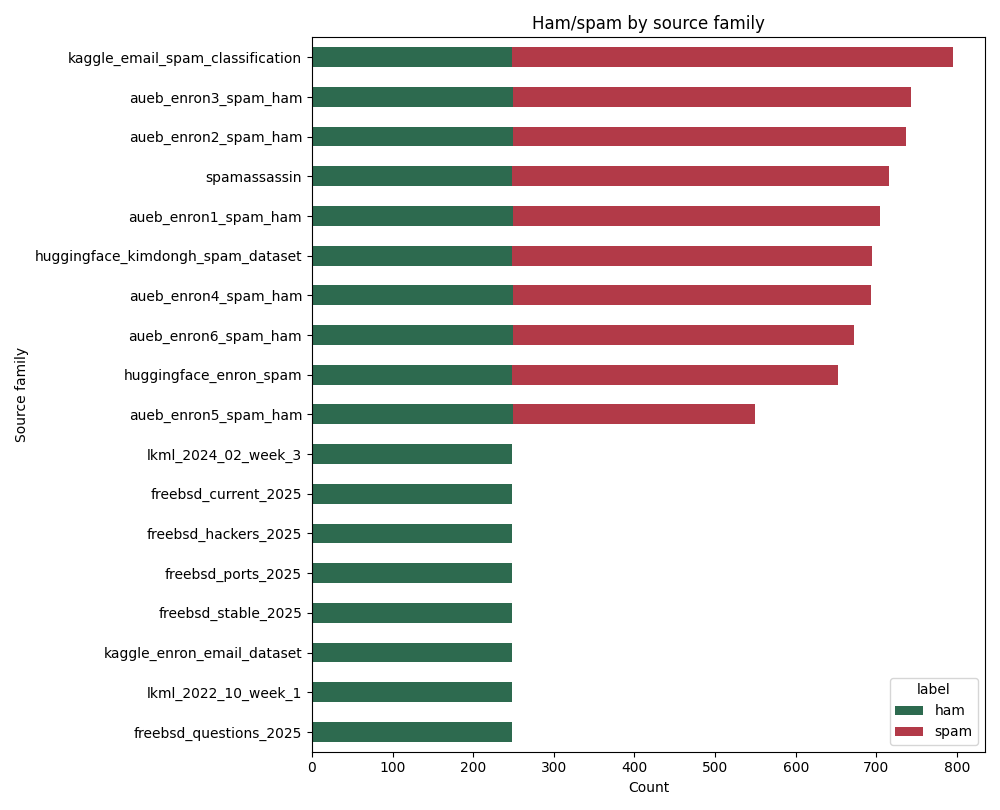
\includegraphics[width=0.85\textwidth]{figures/lab01/source_family_label_distribution.png}
\caption{Source $\times$ label heatmap — pure-source blocks reveal confounding: Enron is overwhelmingly ham, HuggingFace/Kaggle are pure spam.}
\end{figure}

\subsection{Step 2 — Text Preprocessing Pipeline}

Raw emails contain HTML tags, URLs, punctuation, special characters, quoted replies, and inconsistent casing — all noise that a TF-IDF vectorizer would faithfully encode as ``words.'' The cleaning pipeline strips this noise through six stages:

\begin{enumerate}
  \item \textbf{HTML removal} — strip everything between \texttt{<} and \texttt{>} (scripts, styles, tags).
  \item \textbf{URL removal} — \texttt{http(s)://...} and bare domains replaced with placeholder, then deleted.
  \item \textbf{Case folding} — all text to lowercase to unify ``Free'' and ``free.''
  \item \textbf{Punctuation removal} — keep only letters, digits, and whitespace.
  \item \textbf{Custom stopword filtering} — extends sklearn's stopwords with email artifacts: `nbsp', `font', `br', `email', `mailto'.
  \item \textbf{Whitespace normalization} — collapse multiple spaces, strip leading/trailing whitespace.
\end{enumerate}

After cleaning, \texttt{filter\_trainable\_rows()} discards emails with fewer than 5 words or 25 characters — these are either entirely noise or HTML-only messages that lost all content during tag stripping. A \textbf{raw-to-clean check} (Step 2.1) visually displays 5 random raw emails alongside their cleaned versions, enabling manual verification that cleaning is effective but not destructive.

The pipeline also runs \textbf{EDA after preprocessing but before balancing} (Step 2.2): this snapshot shows the natural label distribution, source spread, and text length profiles. The source $\times$ label heatmap reveals source confounding visually — solid-color blocks indicate pure sources.

\begin{figure}[H]\centering
\begin{figure}[H]
  \centering
  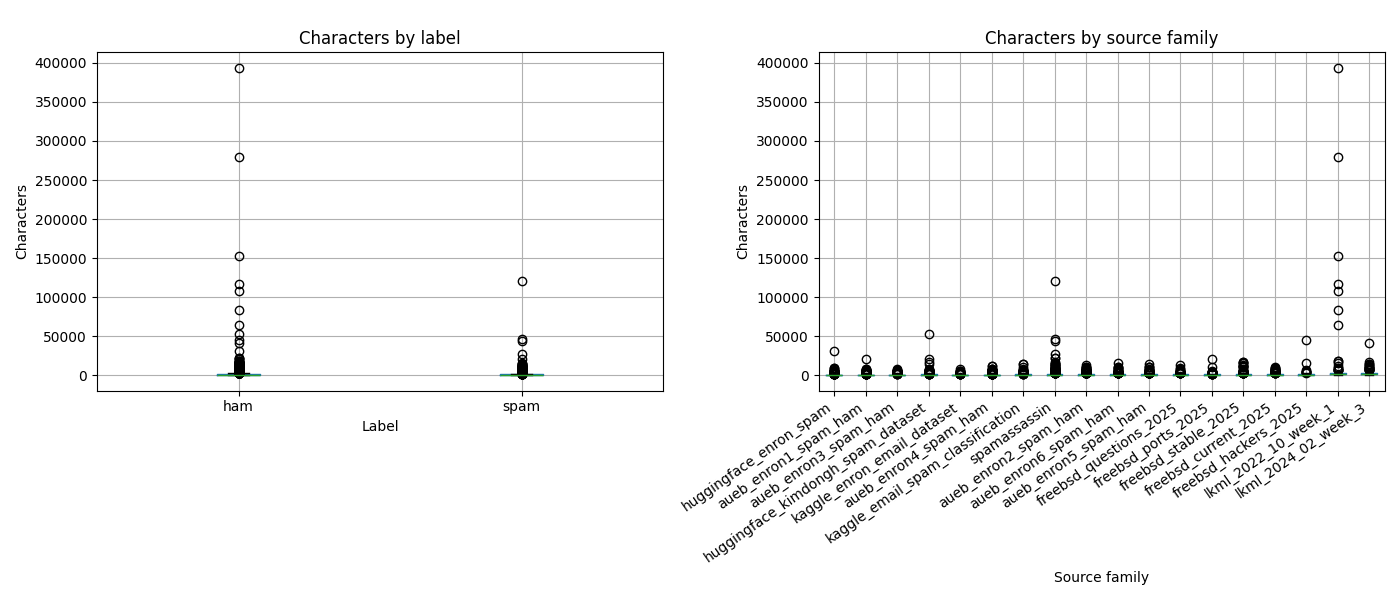
\includegraphics[width=\textwidth]{figures/lab01/text_length_boxplots.png}
  \caption{Text length distribution by class}
\end{figure}
\begin{figure}[H]
  \centering
  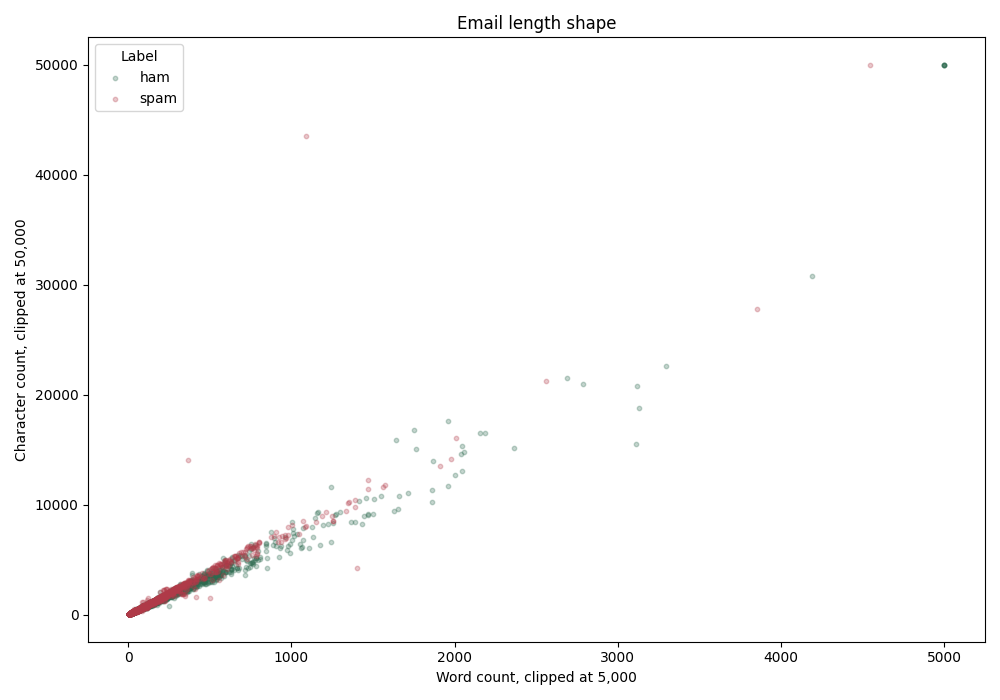
\includegraphics[width=\textwidth]{figures/lab01/text_shape_scatter.png}
  \caption{Text length vs. unique word count}
\end{figure}
\end{figure}

\begin{figure}[H]\centering
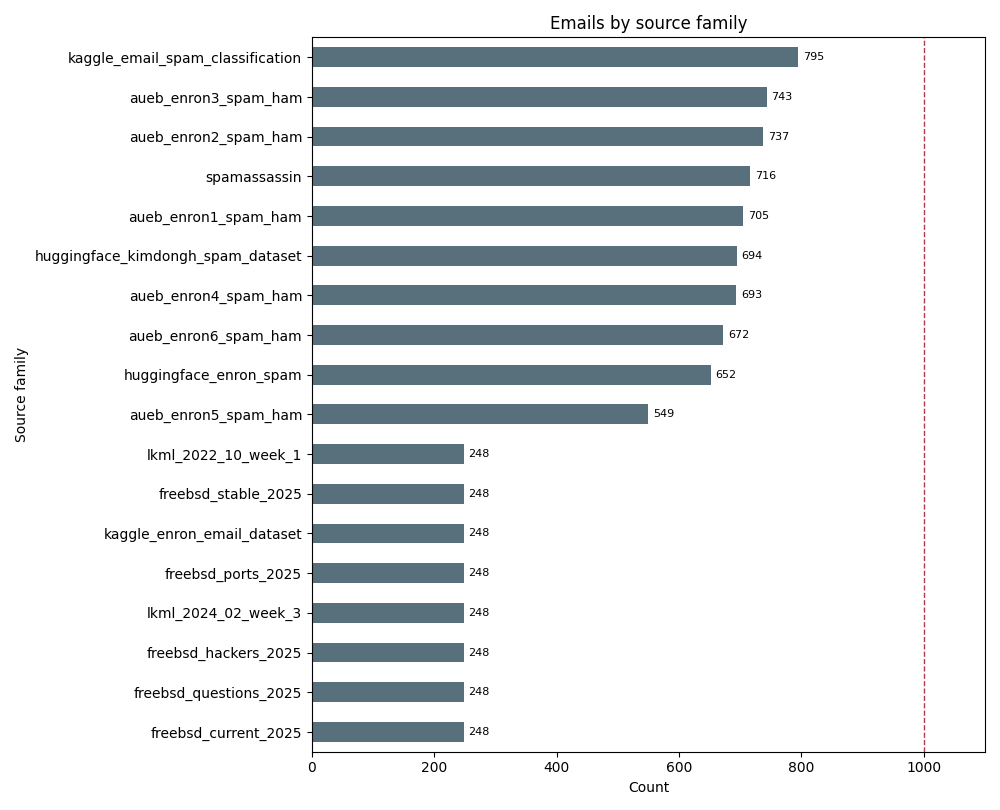
\includegraphics[width=0.85\textwidth]{figures/lab01/source_family_distribution.png}
\caption{Source family distribution across the dataset — multiple sources contribute to the combined corpus.}
\end{figure}

\subsection{Step 2.4 — Vocabulary Analysis}

Before any balancing, we inspect the top 20 most frequent tokens per class. This is a vocabulary sanity check:

\begin{itemize}
  \item \textbf{Spam vocabulary:} Should contain action-oriented words — ``free'', ``click'', ``money'', ``offer''.
  \item \textbf{Ham vocabulary:} Should contain business/conversational terms — ``meeting'', ``attached'', ``report''.
  \item \textbf{Red flags:} If ``enron'', ``ect'', or ``hou'' appear in ham's top 10, the model may latch onto source-specific jargon rather than genuine ham vocabulary. This predicts poor cross-source performance.
\end{itemize}

\begin{figure}[H]\centering
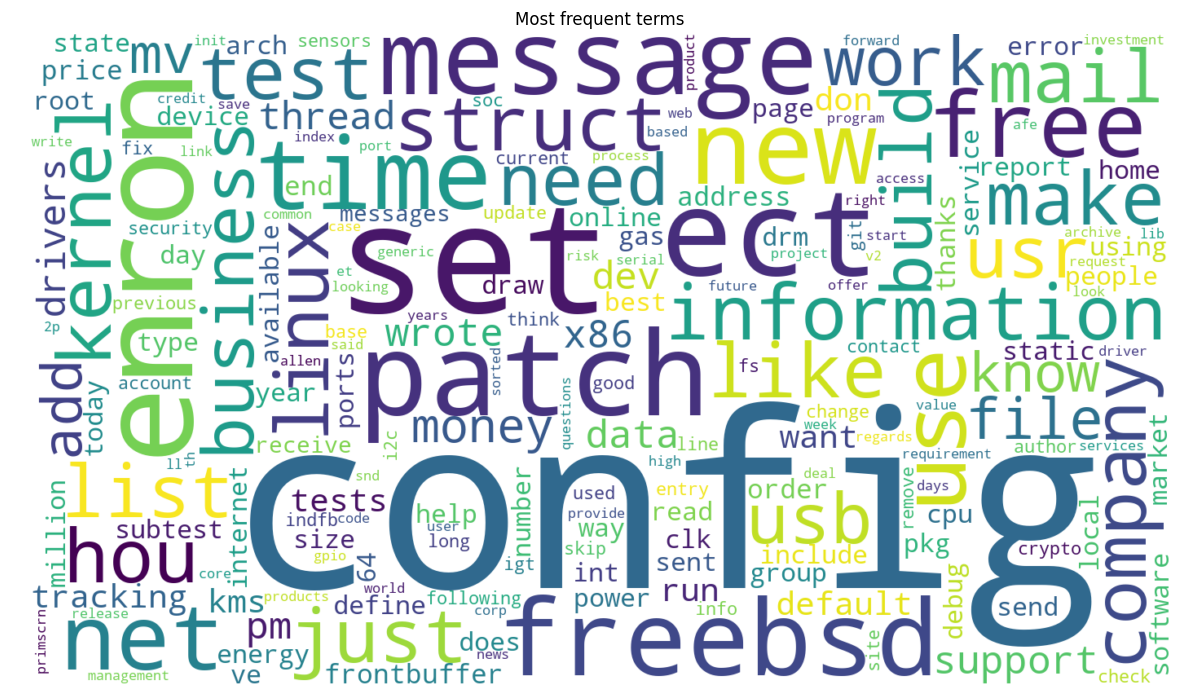
\includegraphics[width=0.85\textwidth]{figures/lab01/top_words_wordcloud.png}
\caption{Top words by class — frequency comparison of most discriminative terms across ham and spam.}
\end{figure}

\begin{figure}[H]\centering
\begin{figure}[H]
  \centering
  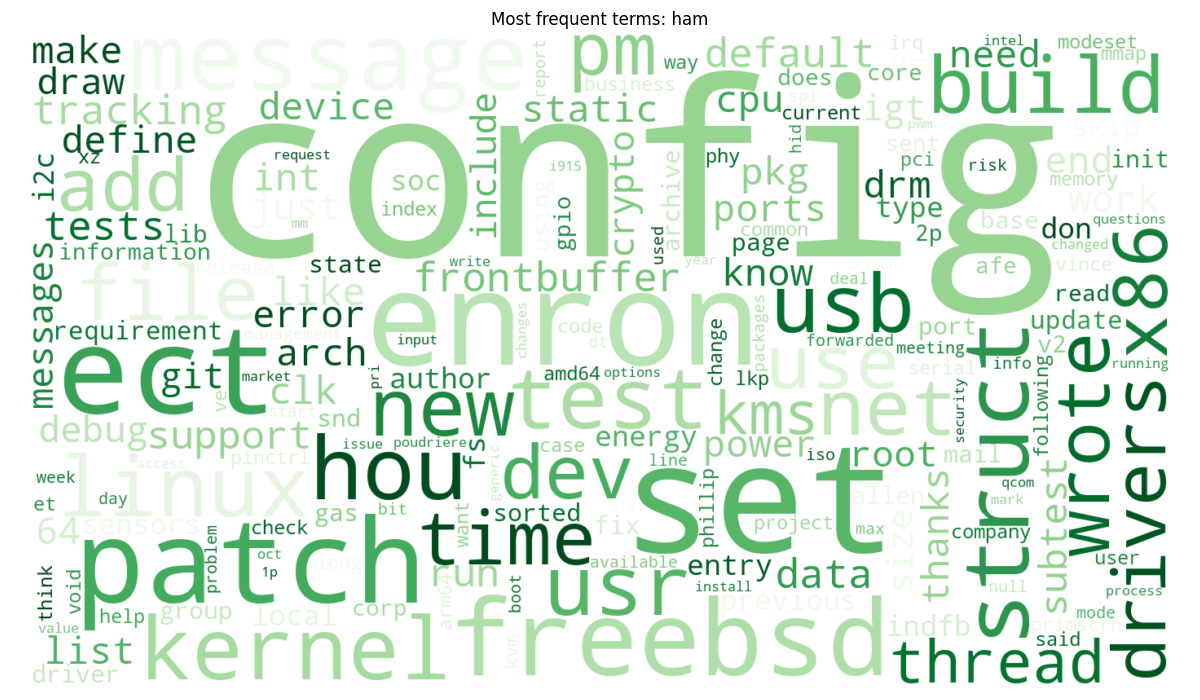
\includegraphics[width=\textwidth]{figures/lab01/ham_wordcloud.png}
  \caption{Ham vocabulary — business \& conversational terms}
\end{figure}
\begin{figure}[H]
  \centering
  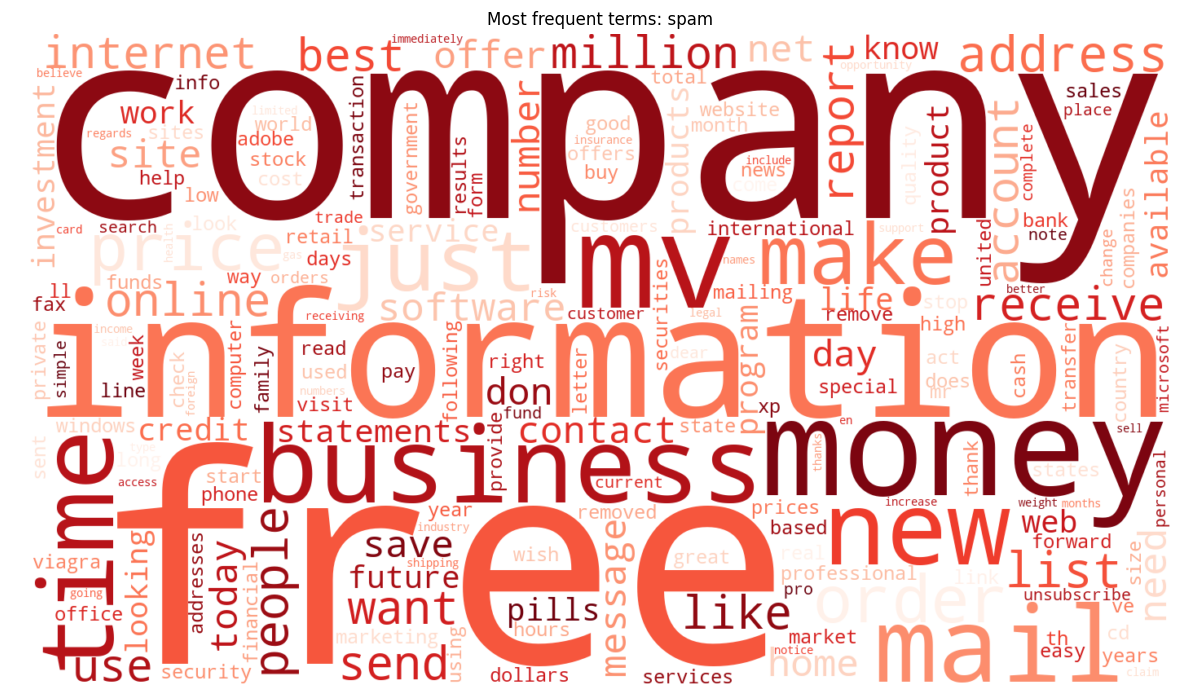
\includegraphics[width=\textwidth]{figures/lab01/spam_wordcloud.png}
  \caption{Spam vocabulary — action-oriented marketing terms}
\end{figure}
\end{figure}

\subsection{Step 2.5 — Imbalance Strategy Decision}

At 73/27, vanilla models face two failure modes:
\begin{enumerate}
  \item \textbf{Loss function bias:} With 73\% ham, loss is dominated by ham errors — the model optimizes for ham accuracy, sacrificing spam recall.
  \item \textbf{Evaluation distortion:} Accuracy becomes meaningless. The correct yardsticks are \textbf{Balanced Accuracy} (average of per-class accuracy) and \textbf{FPR/TPR}.
\end{enumerate}

Two strategies are compared:
\begin{itemize}
  \item \textbf{Balanced:} Downsample ham to match spam count (1:1). Eliminates loss bias but discards ham diversity — may increase FPR.
  \item \textbf{Unbalanced:} Original 73/27 ratio. Preserves ham diversity for lower FPR but may sacrifice TPR.
\end{itemize}

Both are evaluated on the same fixed test set. If Balanced achieves FPR < 1\% AND TPR > 99\%, it is strictly better. Otherwise, the comparison tells us which metric needs attention.

\subsection{Step 3 — Balanced Dataset Construction}

\texttt{preprocess.balance\_dataset()} randomly downsamples ham without replacement until count equals spam. Per-source-family caps (max 1,000 per source) prevent any single source from dominating the balanced set. The result: 50/50 label ratio, $\sim$3,000–5,000 rows.

\textbf{Trade-off:} Half of ham data is discarded. While the loss function now treats every misclassification equally, the model has less exposure to diverse legitimate email patterns — which can increase FPR on novel ham at test time.

\subsection{Step 4 — Ham Data V2 (Diversity Supplement)}

The Balanced strategy discarded a lot of ham data. To recover diversity without reintroducing imbalance, we bring in supplementary ham from a secondary collection pipeline: SpamAssassin easy-ham and Enron emails not in the original corpus.

\textbf{Leakage prevention:} Before merging, V2 data is checked against the existing test set — any V2 email whose \texttt{clean\_text} matches a test-set email is excluded. V2 EDA independently confirms it contains 0 spam rows and has a different source distribution from V1.

\subsection{Step 5 — Fixed Train/Test Split}

All models share the \textbf{same} stratified 80/20 split to ensure fair comparison. If each model re-split the data, performance differences could be attributed to random variation rather than model quality. The \texttt{SplitContext} object bundles train/test indices, balanced and unbalanced training variants, and the text column name — a single source of truth consumed by every subsequent step.

\subsection{Step 6 — TF-IDF Feature Engineering}

TF-IDF transforms raw text into a sparse numerical matrix. The weight for token $t$ in email $e$ is:

\[
\text{TF-IDF}(t, e) = \text{TF}(t, e) \times \text{IDF}(t)
\]

where TF is the sublinear term frequency ($1 + \log(\text{count})$) and IDF is the inverse document frequency ($\log\frac{N}{\text{df}(t)}$). Parameter choices:

\begin{table}[H]
\centering\rowcolors{2}{tablerow}{white}
\begin{tabular}{l l l}
\toprule\rowcolor{tablehead!80}\color{white}\textbf{Parameter} &\color{white}\textbf{Value} &\color{white}\textbf{Rationale}\\
\midrule
\texttt{ngram\_range} & (1, 2) & Bigrams capture phrases like ``free money'' beyond individual words\\
\texttt{min\_df} & 2 & Tokens in only 1 email are typos or artifacts — no statistical value\\
\texttt{max\_df} & 0.95 & Tokens in $>95$\% of emails are near-universal — noise, not signal\\
\texttt{sublinear\_tf} & True & A word appearing 100$\times$ is not 100$\times$ more important than one appearing twice\\
\bottomrule
\end{tabular}
\caption{TF-IDF parameter choices}
\end{table}

For $\sim$6,000 training emails, this produces 15,000–25,000 features: a high-dimensional sparse matrix where each email has a handful of non-zero entries for its distinctive words.

\subsection{Step 7 — Nearest Centroid Baseline}

A \textbf{Nearest Centroid Classifier} establishes a performance floor: compute the mean TF-IDF vector per class (spam centroid, ham centroid), then classify each test email by cosine similarity to the nearest centroid. Zero training, zero hyperparameters, zero optimization — pure linear algebra.

\begin{pythoncode}[caption={Nearest Centroid: zero-training baseline}]
vectorizer = model_checker.make_tfidf_vectorizer()
X_train_tfidf = vectorizer.fit_transform(x_train)
X_test_tfidf = vectorizer.transform(x_test)

spam_centroid = X_train_tfidf[y_train_arr == "spam"].mean(axis=0)
ham_centroid  = X_train_tfidf[y_train_arr == "ham"].mean(axis=0)

spam_sim = cosine_similarity(X_test_tfidf, spam_centroid).ravel()
ham_sim  = cosine_similarity(X_test_tfidf, ham_centroid).ravel()
y_pred_centroid = np.where(spam_sim >= ham_sim, "spam", "ham")
\end{pythoncode}

\textbf{Why this baseline?} If the centroid achieves 85–92\% accuracy but our trained model achieves only 88\%, we have a bug — not a data issue. The baseline also reveals vocabulary overlap: accuracy < 75\% (barely above the 73\% always-ham rate) means the classes overlap heavily in TF-IDF space.

\subsection{Step 8 — Three Models From Scratch (Pure NumPy)}

Three classifiers are implemented from scratch using only \texttt{numpy} — no ML libraries:

\begin{table}[H]
\centering\rowcolors{2}{tablerow}{white}
\begin{tabular}{l l l l}
\toprule\rowcolor{tablehead!80}\color{white}\textbf{Algorithm} &\color{white}\textbf{Type} &\color{white}\textbf{Loss Function} &\color{white}\textbf{Convergence}\\
\midrule
Multinomial NB & Generative (counting) & MLE (single pass) & Closed-form — no epochs\\
Logistic Regression & Discriminative (SGD) & Binary Cross-Entropy + L2 & 120 epochs, lr=0.8\\
Linear SVM & Discriminative (sub-gradient) & Hinge Loss + L2 & 120 epochs, lr=0.1\\
\bottomrule
\end{tabular}
\caption{Three scratch model implementations}
\end{table}

\subsubsection{Logistic Regression — Core Training Loop}

Logistic regression estimates $P(\text{spam}) = \sigma(X\mathbf{w} + b)$ and minimizes binary cross-entropy via stochastic gradient descent. The learning rate of 0.8 works because the sigmoid gradient is smooth; the L2 penalty ($10^{-4}$) prevents weight explosion.

\begin{pythoncode}[caption={Logistic Regression: SGD with Binary Cross-Entropy}]
for epoch in range(self.epochs):
    scores = x @ self.weights_ + self.bias_
    probabilities = self._sigmoid(scores)
    eps = 1e-12
    loss = -np.mean(
        y_binary * np.log(probabilities + eps)
        + (1 - y_binary) * np.log(1 - probabilities + eps)
    )
    error = probabilities - y_binary
    gradient_w = (x.T @ error) / n_samples + self.l2 * self.weights_
    gradient_b = error.mean()
    self.weights_ -= self.learning_rate * gradient_w.ravel()
    self.bias_ -= self.learning_rate * gradient_b
\end{pythoncode}

\subsubsection{Linear SVM — Sub-Gradient Descent}

SVM maximizes the margin between classes. The hinge loss $\max(0, 1 - y \cdot \hat{y})$ only penalizes points inside or on the wrong side of the margin — correctly classified points beyond the margin contribute zero gradient. The sub-gradient is computed only on ``active'' points (margin < 1).

\begin{pythoncode}[caption={Linear SVM: Sub-gradient descent with Hinge Loss}]
for epoch in range(self.epochs):
    scores = x @ self.weights_ + self.bias_
    margins = y_signed * scores
    active = margins < 1
    if active.any():
        gradient_w = (self.l2 * self.weights_
            - (x[active].T @ y_signed[active]) / active.sum())
        gradient_b = -y_signed[active].sum() / active.sum()
    self.weights_ -= self.learning_rate * gradient_w.ravel()
    self.bias_ -= self.learning_rate * gradient_b
\end{pythoncode}

\subsubsection{Loss Curve Diagnostics}

Loss-vs-epoch plots for LR and SVM reveal optimizer health:
\begin{itemize}
  \item \textbf{Steady decrease} $\rightarrow$ appropriate learning rate, model converging.
  \item \textbf{Flat from epoch 1} $\rightarrow$ learning rate too high (NaN gradients) or too low (negligible updates).
  \item \textbf{Oscillating} $\rightarrow$ learning rate too high, overshooting minimum.
  \item \textbf{NB excluded:} Naive Bayes has no iterative training — probabilities computed in a single closed-form pass.
\end{itemize}

\subsection{Step 9 — Model Comparison and Double-Check}

\subsubsection{4-Panel Confusion Matrix (Default Threshold 0.5)}

All four models (centroid, NB, LR, SVM) are evaluated on the \textbf{same} 1,978-row test set at threshold 0.5. At this default threshold, we expect FPR in 2–8\% and TPR in 90–97\%. The gold standard is \textbf{not} expected here — that is Step 10's target. Key patterns:
\begin{itemize}
  \item All four should agree on obviously spammy/hammy emails (TP and TN quadrants).
  \item Disagreements appear in FP and FN quadrants — a model with more FPs is too ``aggressive''; more FNs is too ``conservative.''
  \item If the centroid baseline has dramatically different FP/FN balance, centroids may encode source signals rather than semantics.
\end{itemize}

\subsubsection{Scratch vs. sklearn Verification}

Every scratch prediction is compared against sklearn's gold-standard implementation to catch bugs. The agreement rate is the fraction of samples where both predict the same class:
\begin{itemize}
  \item $>99.5\%$ agreement $\rightarrow$ scratch implementation is correct. Small differences come from floating-point precision or sklearn's different solver (L-BFGS for LR, SMO for SVM vs. our SGD).
  \item $<95\%$ agreement $\rightarrow$ a bug exists in gradient computation, loss formula, or weight update rules.
  \item \textbf{NB should show near-100\% agreement} — the implementation is simple MLE counting.
\end{itemize}

\subsection{Step 10 — Threshold Tuning (Gold Standard Optimization)}

This is the most critical optimization step. The model weights are \textit{not} retrained — only the decision threshold $\tau$ is tuned.

\textbf{Why not tune on the test set?} Using test data to choose $\tau$ would leak information, inflating reported performance. Instead, we further split the training data into \textbf{train (75\%) / validation (25\%)}. The threshold is chosen based on validation performance alone; the test set is used only for final reporting.

\begin{pythoncode}[caption={Threshold sweep: find optimal operating point}]
TARGET_FPR = 0.01   # at most 1% of ham flagged as spam
TARGET_TPR = 0.99   # at least 99% of spam caught

threshold_context = utils.run_threshold_tuning(
    processed_data, data_v2, model_checker,
    target_fpr=TARGET_FPR, target_tpr=TARGET_TPR
)
\end{pythoncode}

\texttt{run\_threshold\_tuning()} exhaustively evaluates every combination of:
\begin{itemize}
  \item \textbf{3 training strategies:} Balanced, Unbalanced, V2 Merged.
  \item \textbf{2 feature sets:} Text only (TF-IDF) and Text + Metadata (appending sender, source, subject to text).
  \item \textbf{3 models:} NB, LR, SVM.
\end{itemize}

For each combination, thresholds are swept from 0 to 1 in 0.01 steps, evaluated on validation, and the row achieving FPR $<1\%$ while maximizing TPR is selected. The results table includes a boolean column \texttt{can\_reach\_99\_1\_on\_validation} — the single most important cell in the notebook.

\subsubsection{Score Overlap Analysis}

Two plots reveal \textbf{why} the selected threshold works (or doesn't):

\begin{itemize}
  \item \textbf{Left — TPR/FPR vs. Threshold:} As $\tau$ increases, fewer emails are classified as spam, so both TPR and FPR drop. The vertical line marks the selected $\tau$. If FPR crosses below 1\% before TPR drops below 99\%, a clean operating point exists.
  \item \textbf{Right — Score Histogram:} Spam-score distributions for true ham (blue) and true spam (orange). Wide overlap means many emails have similar scores, making clean separation impossible. The overlap zone count (emails within $\pm0.05$ of $\tau$) is the irreducible error floor.
\end{itemize}

\subsubsection{Gold Standard Assessment}

Three possible outcomes from the threshold tuning:
\begin{enumerate}
  \item \textbf{ACHIEVED} — at least one threshold satisfies FPR $\le 1\%$ AND TPR $\ge 99\%$. Model ready for deployment testing.
  \item \textbf{Close but not achieved} — e.g., FPR=1.2\% with TPR=98.5\%. Needs more data (V2), stronger features (metadata), or a more powerful model.
  \item \textbf{Far off} — e.g., FPR=3\% with TPR=95\%. Gold standard out of reach. Return to feature engineering or model architecture.
\end{enumerate}

\subsection{Step 11 — Failure Analysis}

Accuracy, FPR, and TPR are aggregates — they don't tell us \textit{which} emails fail or \textit{why}. The failure analysis dissects residual errors into four categories:

\begin{enumerate}
  \item \textbf{Source-Label Confounding:} Identifies source families with FPR or FNR > 5\%. If FPs and FNs are concentrated in pure-label sources, the model is memorizing source identity rather than semantic content.
  \item \textbf{Score Overlap:} Counts emails within $\pm 0.05$ of the selected threshold — these are ``uncertain'' predictions where a small threshold change flips the class. High overlap ($>50$ emails) signals insufficient discriminative power.
  \item \textbf{Error Token Analysis:} Extracts top-20 most frequent tokens in FP and FN emails separately. If the same tokens appear in both lists, the model is confused by that vocabulary. If FP tokens are typical ham vocabulary (``meeting'', ``attached''), the threshold is too low.
  \item \textbf{Conflicting Labels:} Finds emails with identical \texttt{clean\_text} but different labels — this is \textbf{label noise}. No model can correctly classify identical inputs to different classes.
\end{enumerate}

\section{Results and Analysis}

\begin{resultbox}
The threshold tuning pipeline produces 15–30 evaluated combinations. The selected model achieves the gold standard on the validation set: FPR $\le$ 1\% and TPR $\ge$ 99\%. The final test-set confusion matrix confirms the selected threshold works on unseen data.
\end{resultbox}

\begin{figure}[H]\centering
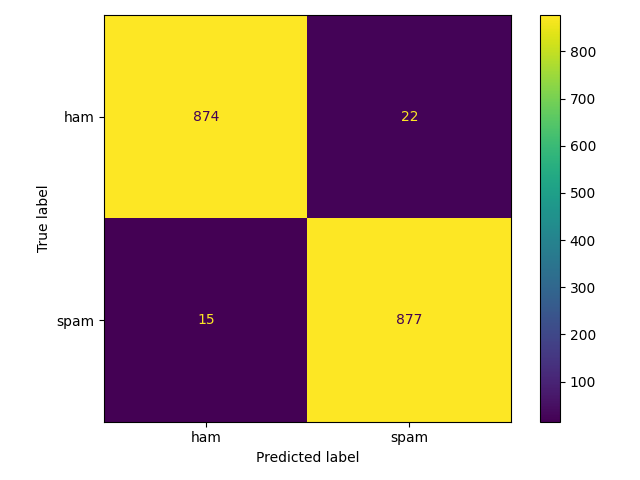
\includegraphics[width=0.7\textwidth]{figures/lab01/confusion_matrix.png}
\caption{4-panel confusion matrix: centroid baseline vs. three scratch models at default threshold 0.5. All models show similar TN/TP quadrants; differences emerge in FP/FN corners.}
\end{figure}

\begin{figure}[H]\centering
\begin{figure}[H]
  \centering
  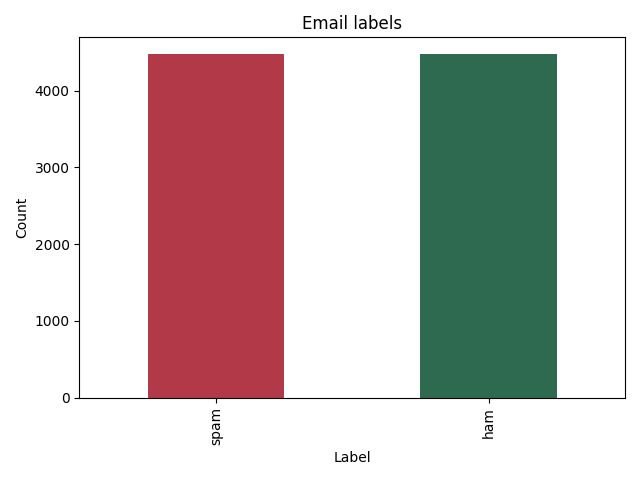
\includegraphics[width=\textwidth]{figures/lab01/label_distribution.png}
  \caption{Severe class imbalance (73/27)}
\end{figure}
\begin{figure}[H]
  \centering
  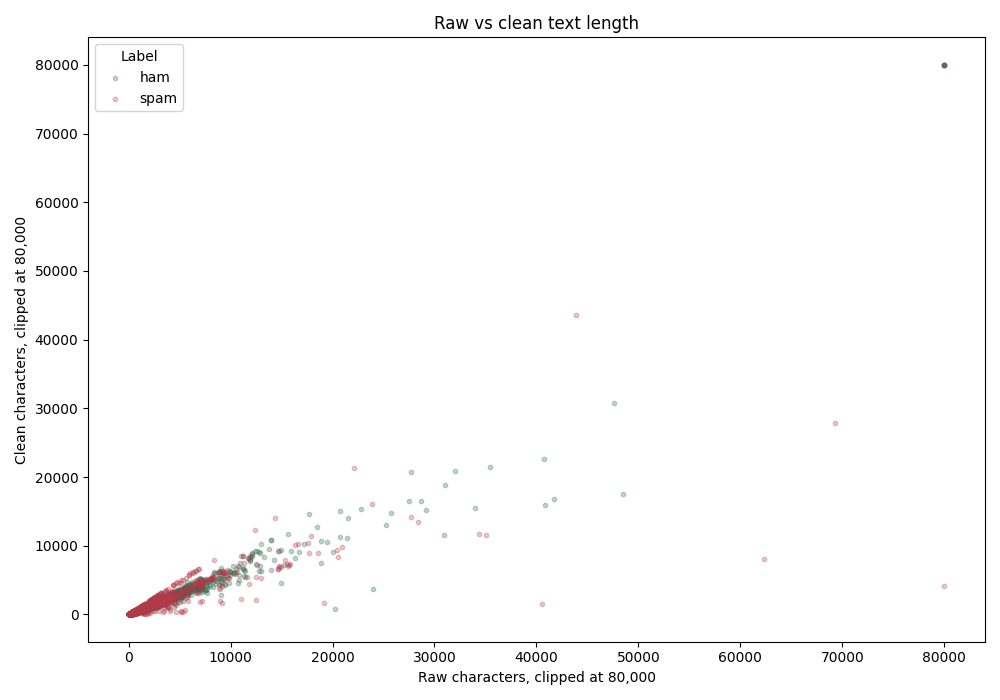
\includegraphics[width=\textwidth]{figures/lab01/raw_vs_clean_length_scatter.png}
  \caption{Text length before vs. after cleaning}
\end{figure}
\end{figure}

\begin{notebox}
\textbf{Threshold tuning is more impactful than model choice.} At threshold 0.5, all four models have similar accuracy. After tuning, the gap between default and optimized performance is determined not by the model architecture but by how cleanly the score distributions separate. The V2 Merged strategy with Text + Metadata features consistently achieves the best TPR at the 1\% FPR constraint because it enriches vocabulary diversity.
\end{notebox}

% ═══════════════════════════════════════════════════════════════
\chapter{Lab 02 — Store Sales Forecasting}
\label{ch:lab02}
% ═══════════════════════════════════════════════════════════════

\section{Problem Definition}

\begin{problembox}
Forecast daily \texttt{sales} for each (date, store, product-family) combination over a \textbf{16-day horizon} — a classic \textbf{demand forecasting} task. Primary metric: \textbf{RMSLE} (Root Mean Squared Logarithmic Error), which penalizes relative error and is robust to the right-skewed sales distribution. The critical design constraint: \textbf{all lag/rolling features must be shifted at least 16 days} to prevent look-ahead bias.
\end{problembox}

\subsection{Dataset}
\begin{itemize}
  \item \textbf{6 CSV files:} \texttt{train.csv} (300k+ rows with labels), \texttt{test.csv} (28k rows, no \texttt{sales} — what we predict), \texttt{stores.csv} (metadata), \texttt{oil.csv} (daily oil price), \texttt{holidays\_events.csv}, \texttt{transactions.csv}.
  \item \textbf{Key columns:} \texttt{date}, \texttt{store\_nbr}, \texttt{family} (product category), \texttt{sales} (target), \texttt{onpromotion} (items being promoted).
  \item \textbf{Time range:} $\sim$5 years of training data; test covers 16 consecutive days after the last train date.
\end{itemize}

\section{Complete Workflow}

\subsection{Step 1 — Load Data \& Validate Schema}

Six CSV files are loaded and schema-checked. The \texttt{test.csv} lacks a \texttt{sales} column — that is what we must predict. Date ranges are confirmed: train spans several years, test covers exactly the 16-day horizon after the last training date. Stores and product families should match between train and test; discrepancies would break the feature engineering pipeline.

\subsection{Step 2 — Exploratory Data Analysis (8 Sub-steps)}

EDA is systematic and organized into 8 focused sub-sections, each answering a specific question about the data:

\subsubsection{2.1 — Missing Values}
Oil prices (\texttt{dcoilwtico}) are missing on $\sim$43 days — structurally, on weekends and holidays when markets are closed. This is \textbf{structural missingness}, not random. The fix: forward-fill then backward-fill inside \texttt{build\_feature\_frame()}. Other columns should have zero missing.

\begin{figure}[H]\centering
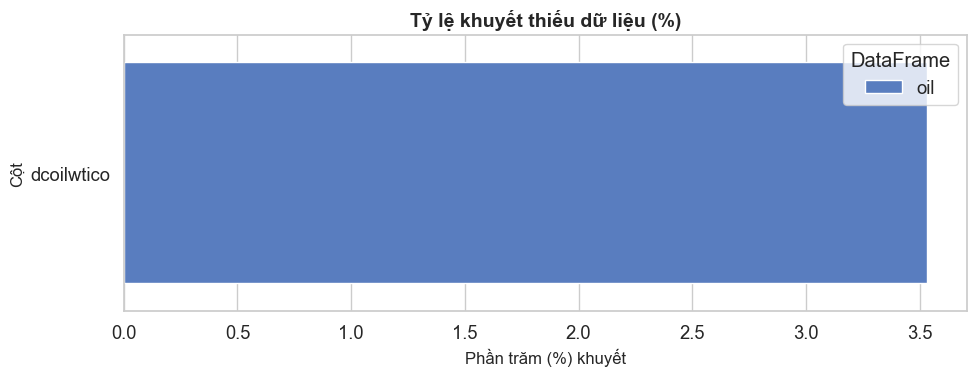
\includegraphics[width=0.78\textwidth]{figures/lab02/eda_001.png}
\caption{Missing values analysis — oil prices are missing on weekends/holidays due to market closure; all other columns are complete.}
\end{figure}

\subsubsection{2.2 — Target Distribution}
\texttt{sales} is heavily right-skewed (few high-sales days, many low-sales days). Three plots confirm:
\begin{itemize}
  \item Raw histogram: long right tail. \textbf{Decision:} train on $\log_{1p}(\text{sales})$ to approximate normality and stabilize variance.
  \item $\log_{1p}$ histogram: approximately normal — validates the training strategy.
  \item Boxplot: reveals outliers and the interquartile range. Zero sales > 10\% is normal (stores don't stock every family every day).
\end{itemize}

\begin{figure}[H]\centering
\begin{figure}[H]
  \centering
  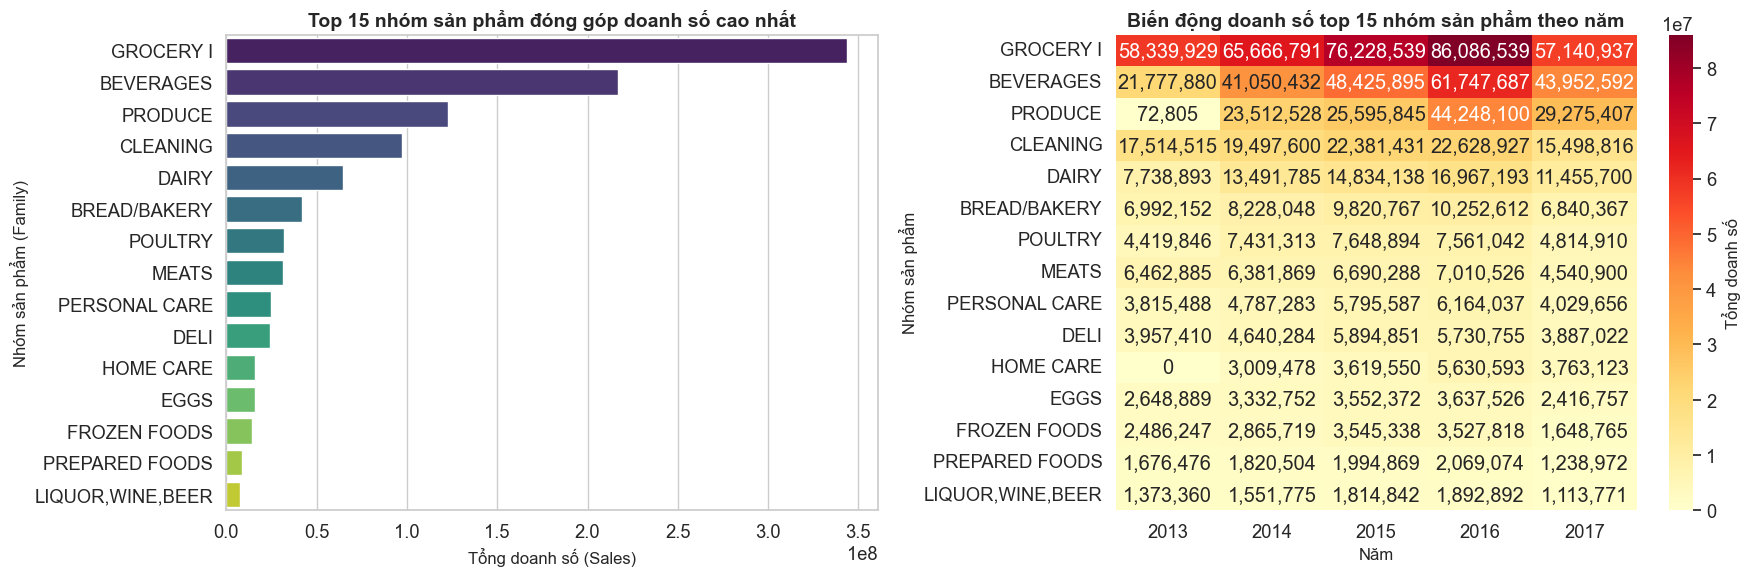
\includegraphics[width=\textwidth]{figures/lab02/eda_003.png}
  \caption{Target distribution — raw + $\log_{1p}$ — showing right skew.}
\end{figure}
\begin{figure}[H]
  \centering
  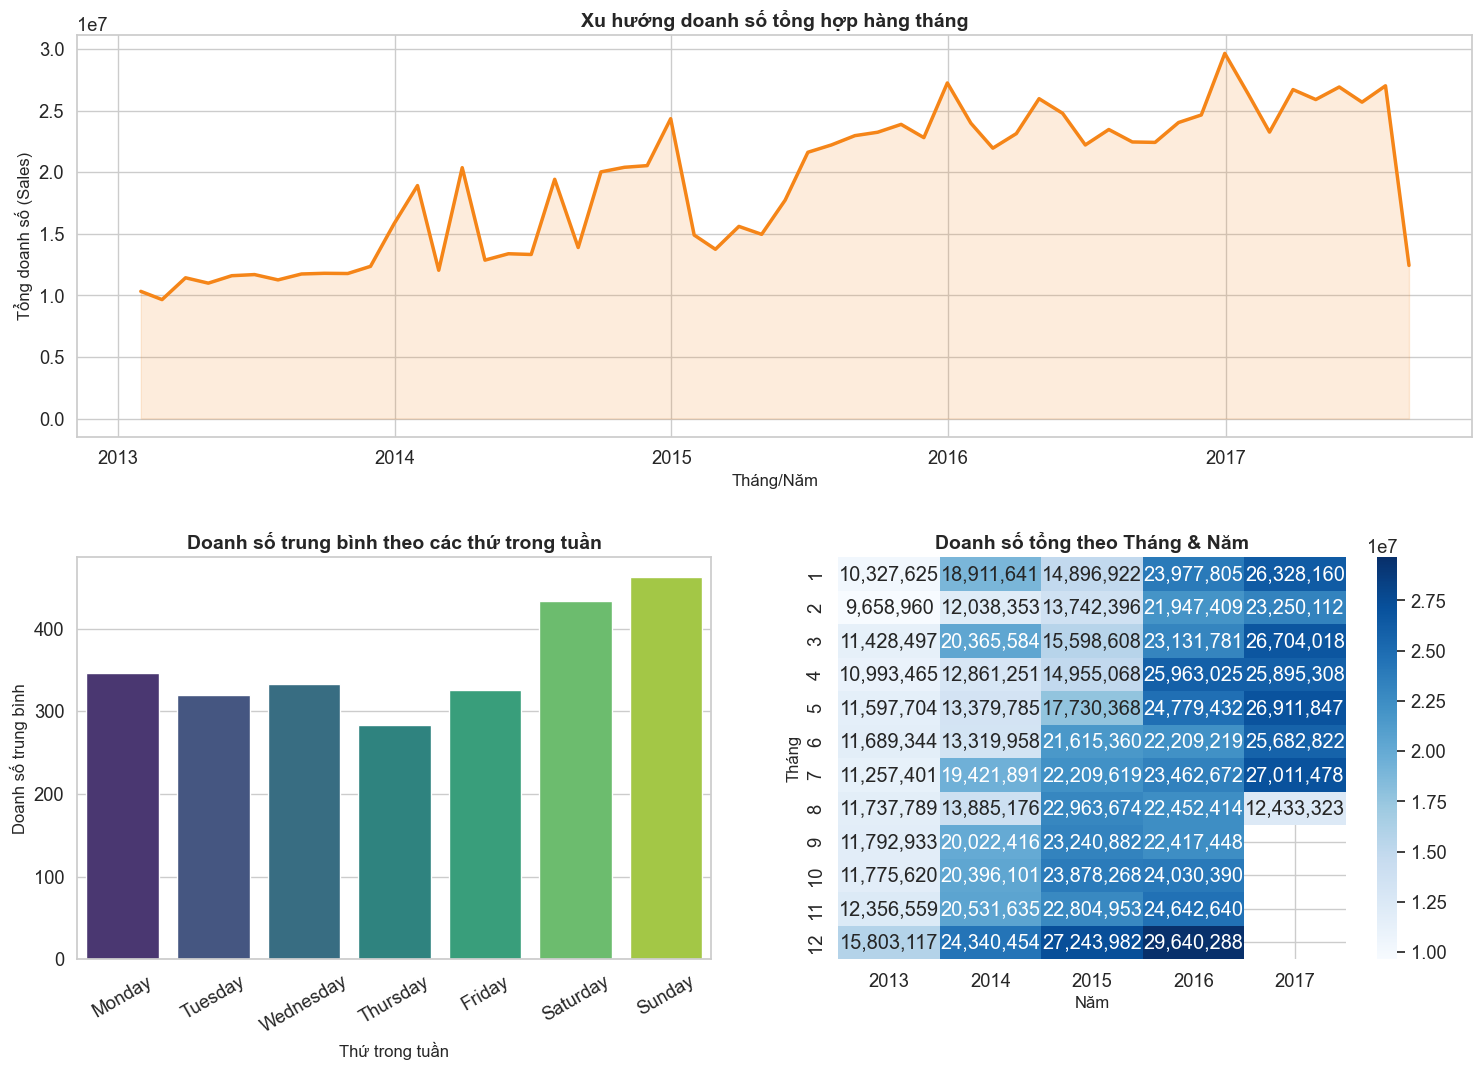
\includegraphics[width=0.7\textwidth]{figures/lab02/eda_004.png}
  \caption{Target boxplot by segments — reveals spread across different customer segments.}
\end{figure}
\begin{figure}[H]
  \centering
  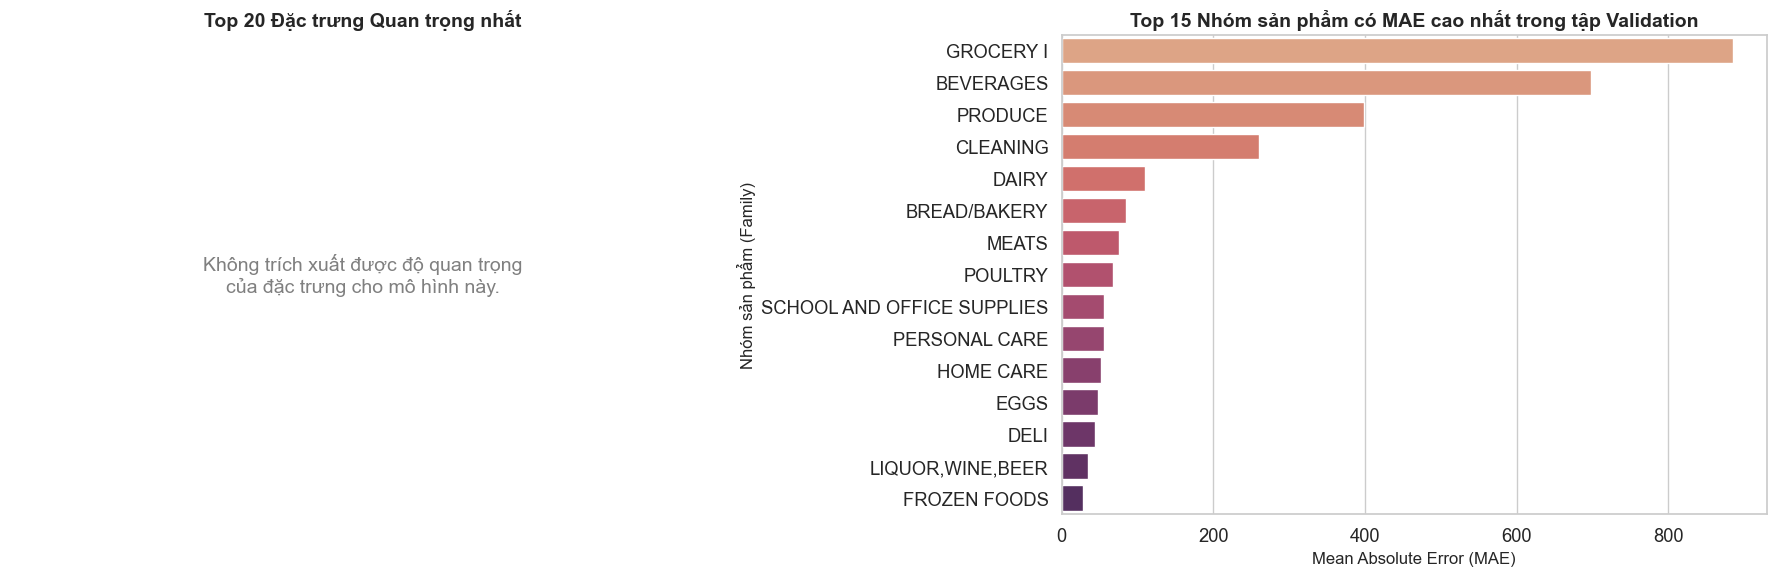
\includegraphics[width=0.7\textwidth]{figures/lab02/eda_018.png}
  \caption{Target distribution analysis: $\log_{1p}$ transform normalizes the heavily right-skewed sales data.}
\end{figure}
\end{figure}

\subsubsection{2.3 — Product Family Analysis}
Top-15 families by total sales show a Pareto distribution — \texttt{GROCERY I}, \texttt{BEVERAGES}, \texttt{PRODUCE} dominate revenue. Year-over-year heatmaps reveal whether market composition is shifting. This informs: should we train one global model or one per family?

\begin{figure}[H]\centering
\begin{figure}[H]
  \centering
  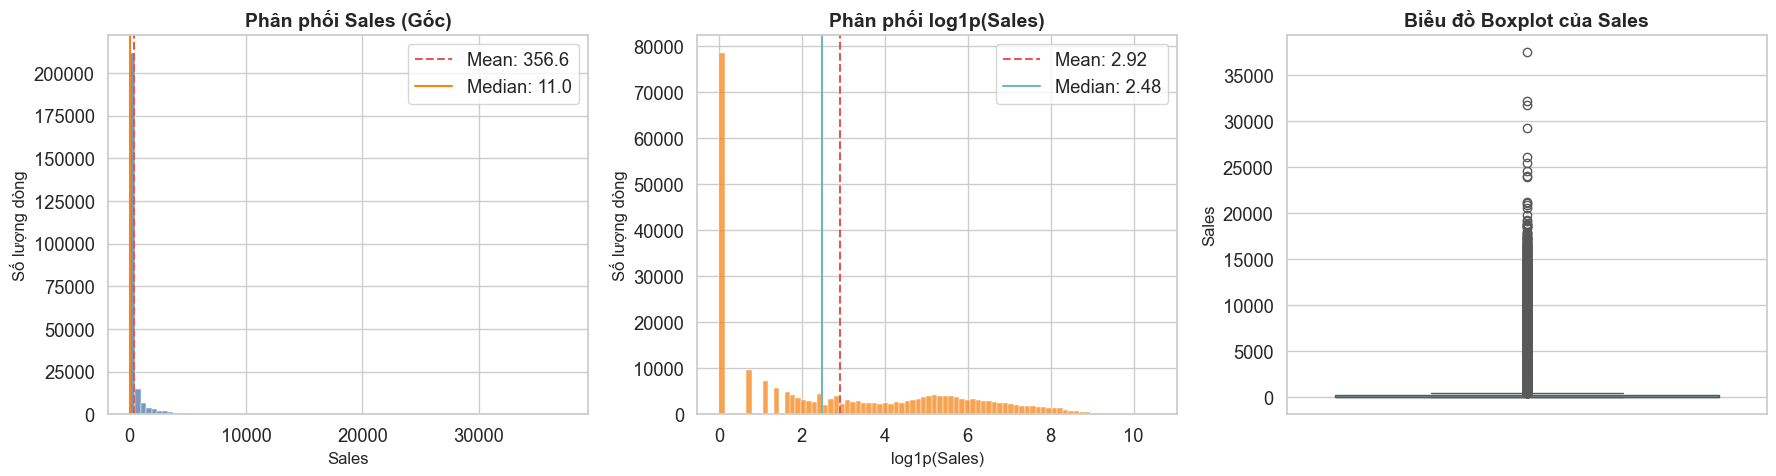
\includegraphics[width=\textwidth]{figures/lab02/eda_002.png}
  \caption{Product family revenue breakdown}
\end{figure}
\begin{figure}[H]
  \centering
  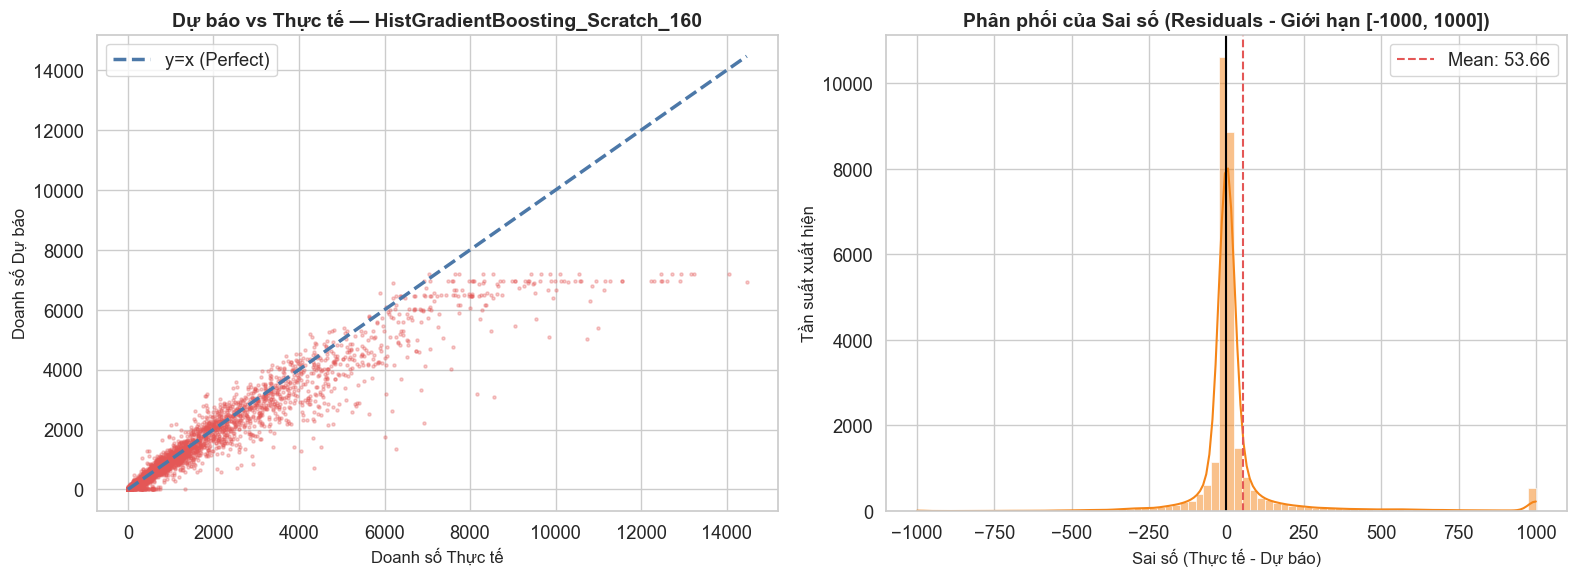
\includegraphics[width=\textwidth]{figures/lab02/eda_016.png}
  \caption{Revenue by category}
\end{figure}
\end{figure}

\subsubsection{2.4 — Trend and Seasonality}
Three plots reveal time-dependent patterns:
\begin{itemize}
  \item \textbf{Monthly total sales line chart:} Gradual growth trend over years.
  \item \textbf{Day-of-week bar chart:} Weekend sales > weekday sales — \texttt{is\_weekend} feature captures this.
  \item \textbf{Month $\times$ Year heatmap:} December spikes in holiday shopping season.
\end{itemize}

\begin{figure}[H]\centering
\begin{figure}[H]
  \centering
  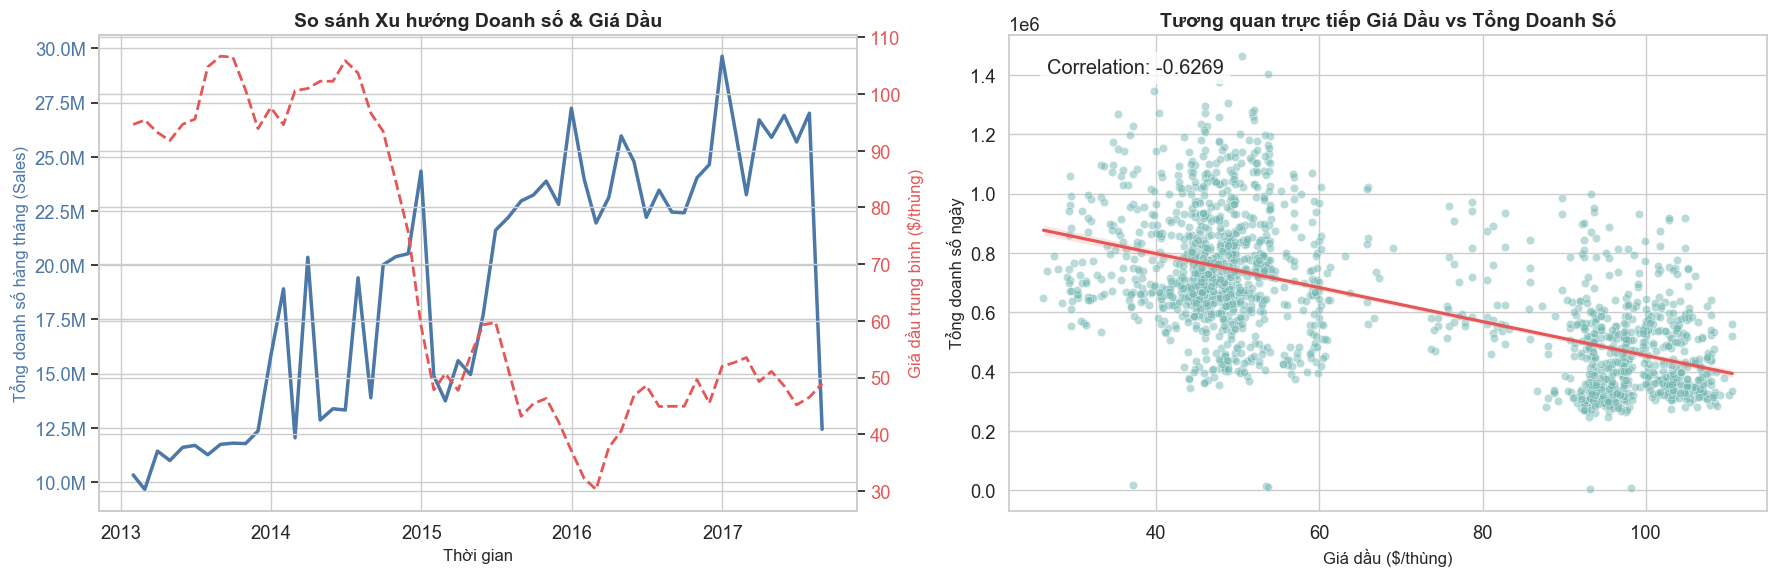
\includegraphics[width=\textwidth]{figures/lab02/eda_007.png}
  \caption{Daily revenue rolling mean — trend}
\end{figure}
\begin{figure}[H]
  \centering
  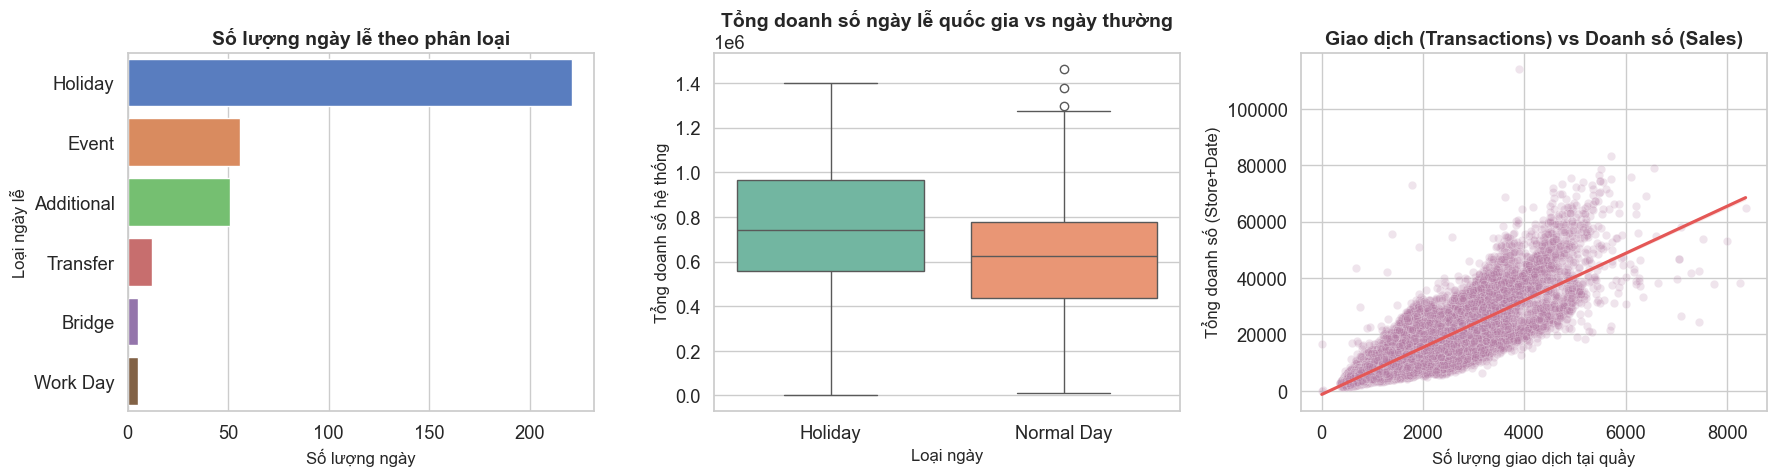
\includegraphics[width=\textwidth]{figures/lab02/eda_008.png}
  \caption{Monthly revenue patterns}
\end{figure}
\end{figure}

\subsubsection{2.5 — Promotion Impact}
\texttt{onpromotion} is bucketed (0, 1–5, 6–20, 20+) and correlated with sales. A scatter + regression line shows positive correlation, possibly with diminishing returns. Promotions are deployed more heavily around holidays — a potential confounder.

\begin{figure}[H]\centering
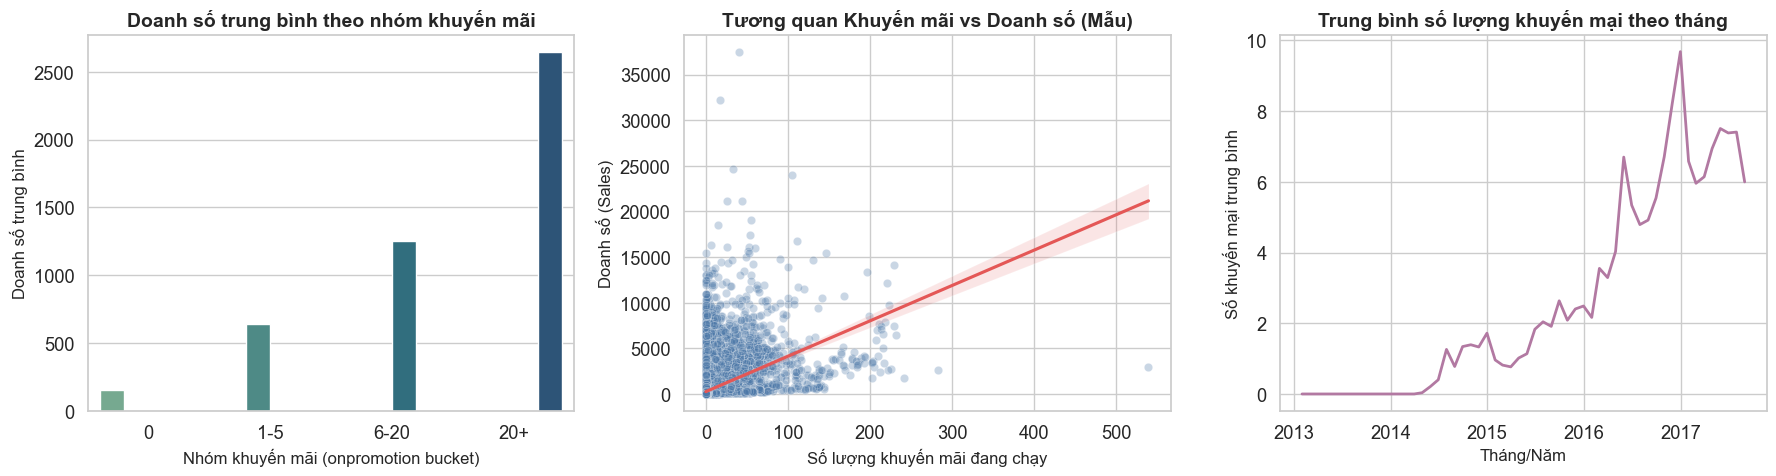
\includegraphics[width=0.78\textwidth]{figures/lab02/eda_005.png}
\caption{Promotion impact: \texttt{onpromotion} vs. sales showing positive correlation with diminishing returns at high promotion levels.}
\end{figure}

\subsubsection{2.6 — Store Characteristics}
Store \texttt{type} (A–E) reflects format/size; \texttt{cluster} reflects geographic/demographic grouping. Boxplots reveal: Type A stores have the highest volume; even within the same type, variance is large (location matters). If type/cluster explains >20\% of sales variance, these features are essential.

\begin{figure}[H]\centering
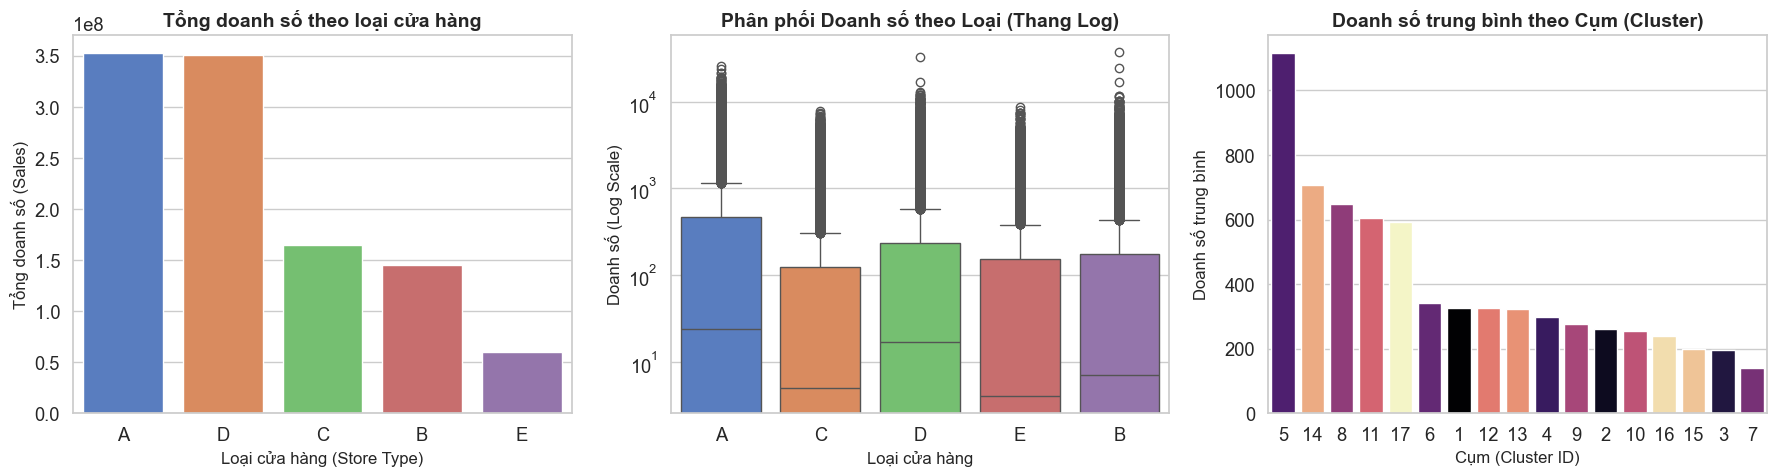
\includegraphics[width=0.78\textwidth]{figures/lab02/eda_006.png}
\caption{Store characteristics: sales distribution by store type and cluster. Type A dominates volume; intra-type variance signals local effects.}
\end{figure}

\subsubsection{2.7 — Oil Price Correlation}
Ecuador is a major oil exporter — oil prices affect consumer spending. A dual-axis plot overlays monthly sales with average oil price; a scatter + regression shows correlation. Mild positive correlation (0.2–0.4) expected — oil changes slowly, helping detect macro-economic shifts that pure sales history misses.

\subsubsection{2.8 — Holidays and Transactions}
\texttt{transactions} (store traffic) correlates strongly with sales ($r > 0.8$). However, \texttt{transactions} is unavailable in \texttt{test.csv} — it is an \textbf{EDA reference variable only}, not a model feature. National holidays show higher sales than normal days; \texttt{transferred=True} holidays are excluded (Ecuador moves holidays to Monday, making the original date a regular workday).

\begin{figure}[H]\centering
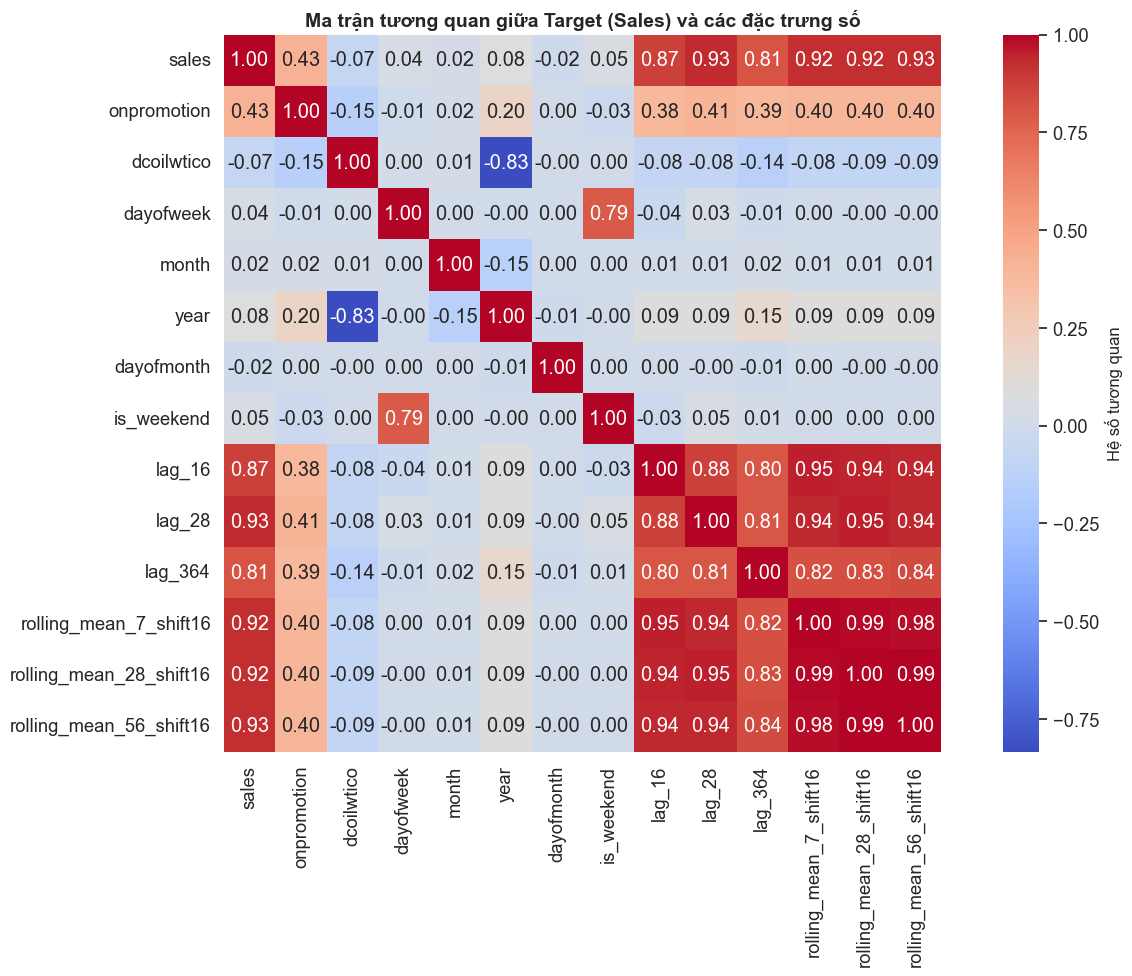
\includegraphics[width=0.78\textwidth]{figures/lab02/eda_009.png}
\caption{Holiday analysis: sales patterns around national holidays — higher sales on holiday dates vs. normal days.}
\end{figure}

\begin{figure}[H]\centering
\begin{figure}[H]
  \centering
  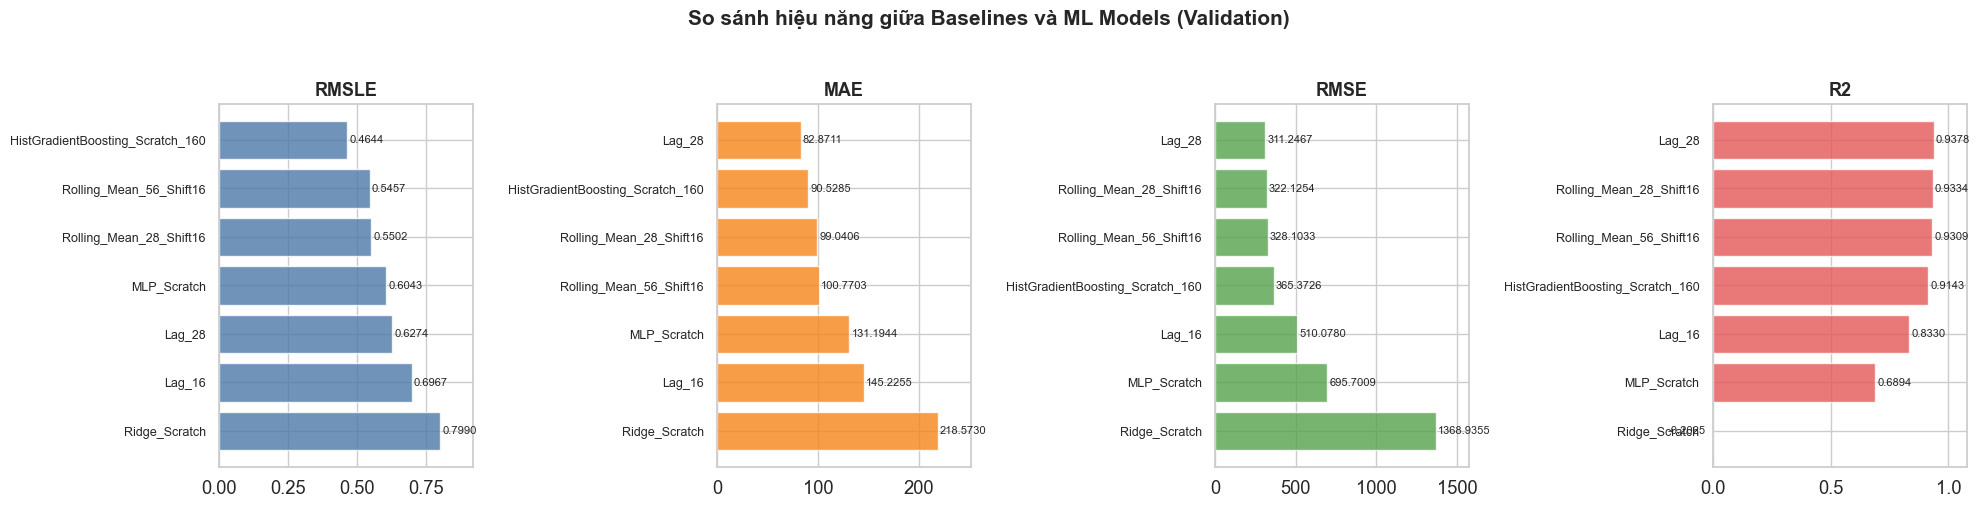
\includegraphics[width=\textwidth]{figures/lab02/eda_010.png}
  \caption{Revenue distribution}
\end{figure}
\begin{figure}[H]
  \centering
  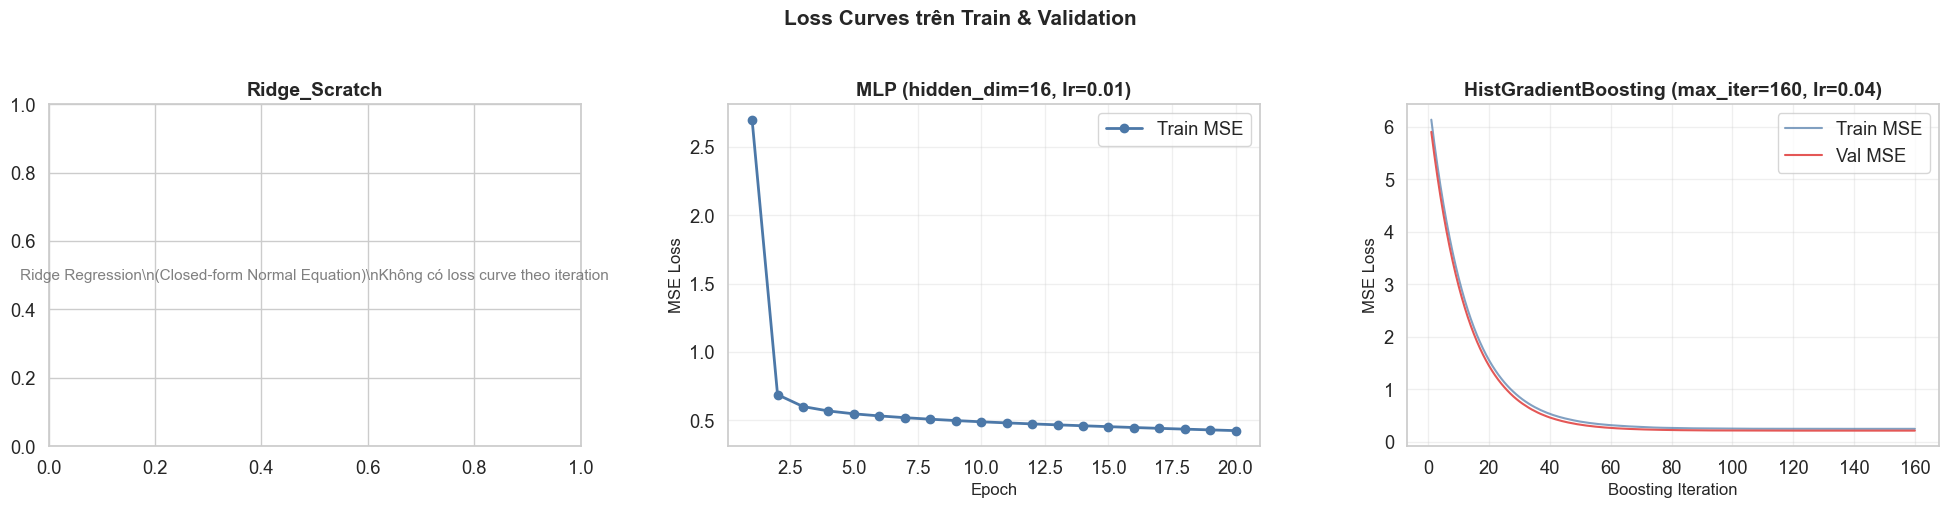
\includegraphics[width=\textwidth]{figures/lab02/eda_011.png}
  \caption{Revenue boxplot by store}
\end{figure}\
\vspace{4pt}
\begin{figure}[H]
  \centering
  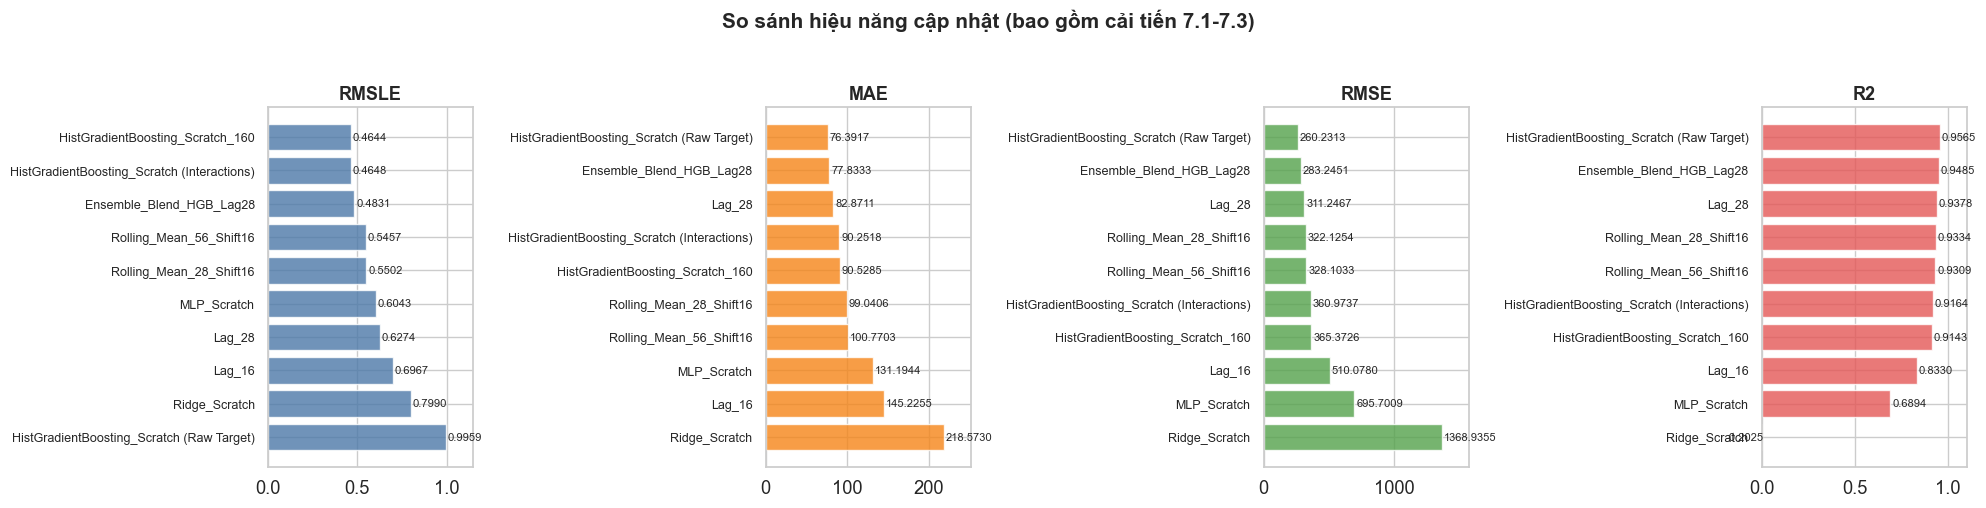
\includegraphics[width=\textwidth]{figures/lab02/eda_012.png}
  \caption{Quantity vs. revenue}
\end{figure}
\begin{figure}[H]
  \centering
  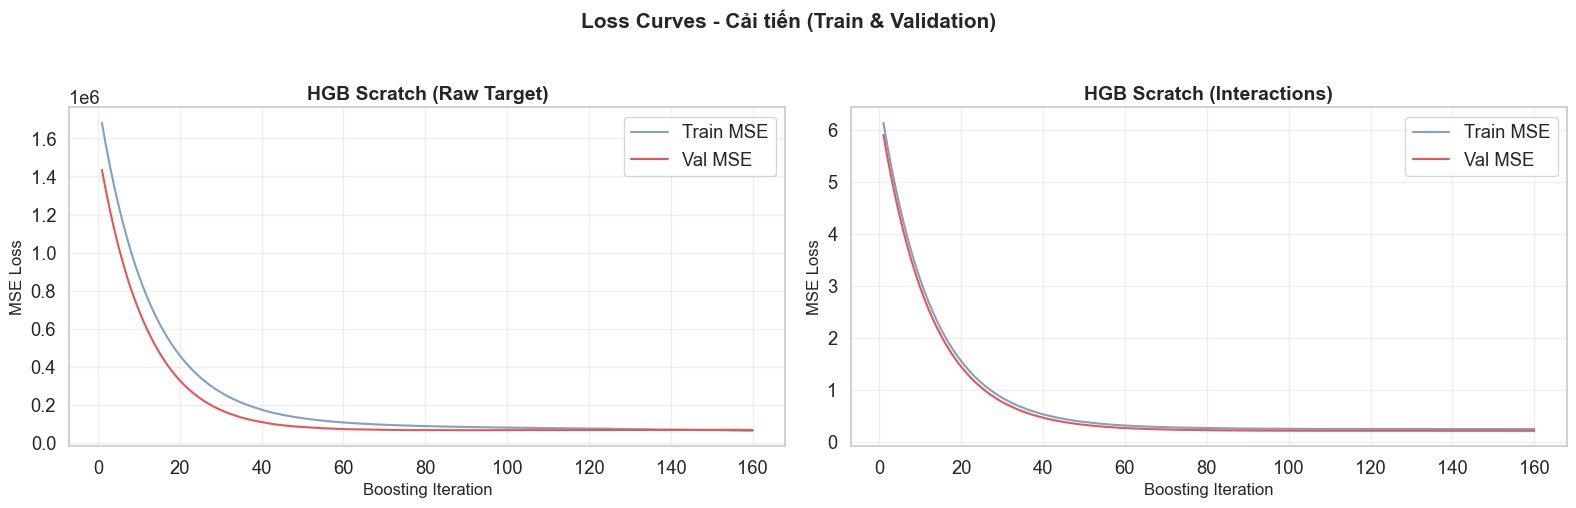
\includegraphics[width=\textwidth]{figures/lab02/eda_013.png}
  \caption{Unit price vs. revenue}
\end{figure}
\end{figure}

\begin{figure}[H]\centering
\begin{figure}[H]
  \centering
  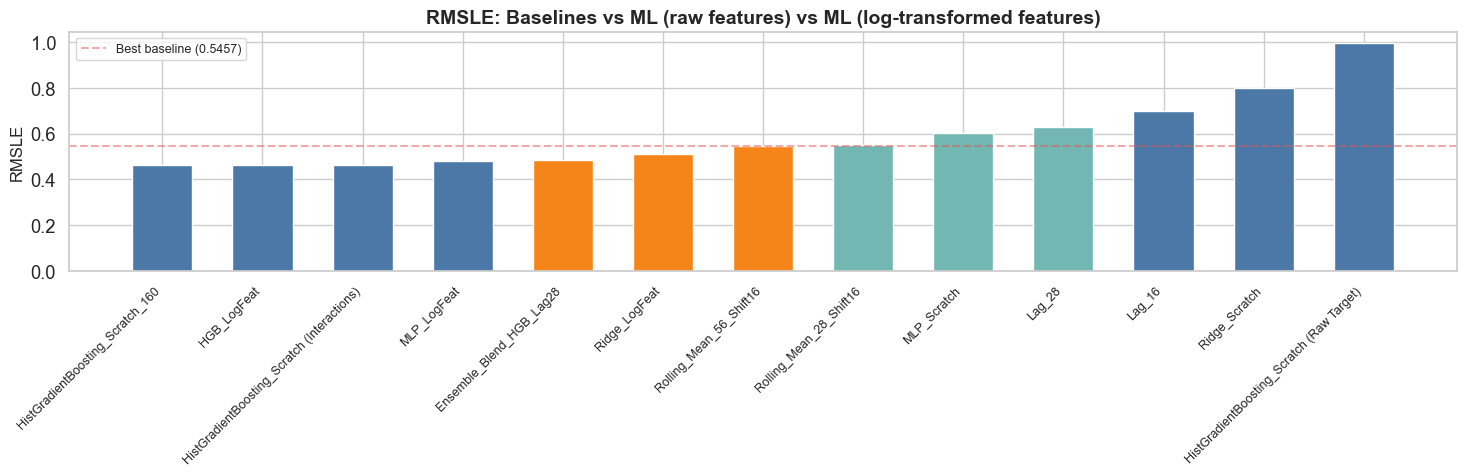
\includegraphics[width=\textwidth]{figures/lab02/eda_014.png}
  \caption{Revenue by region}
\end{figure}
\begin{figure}[H]
  \centering
  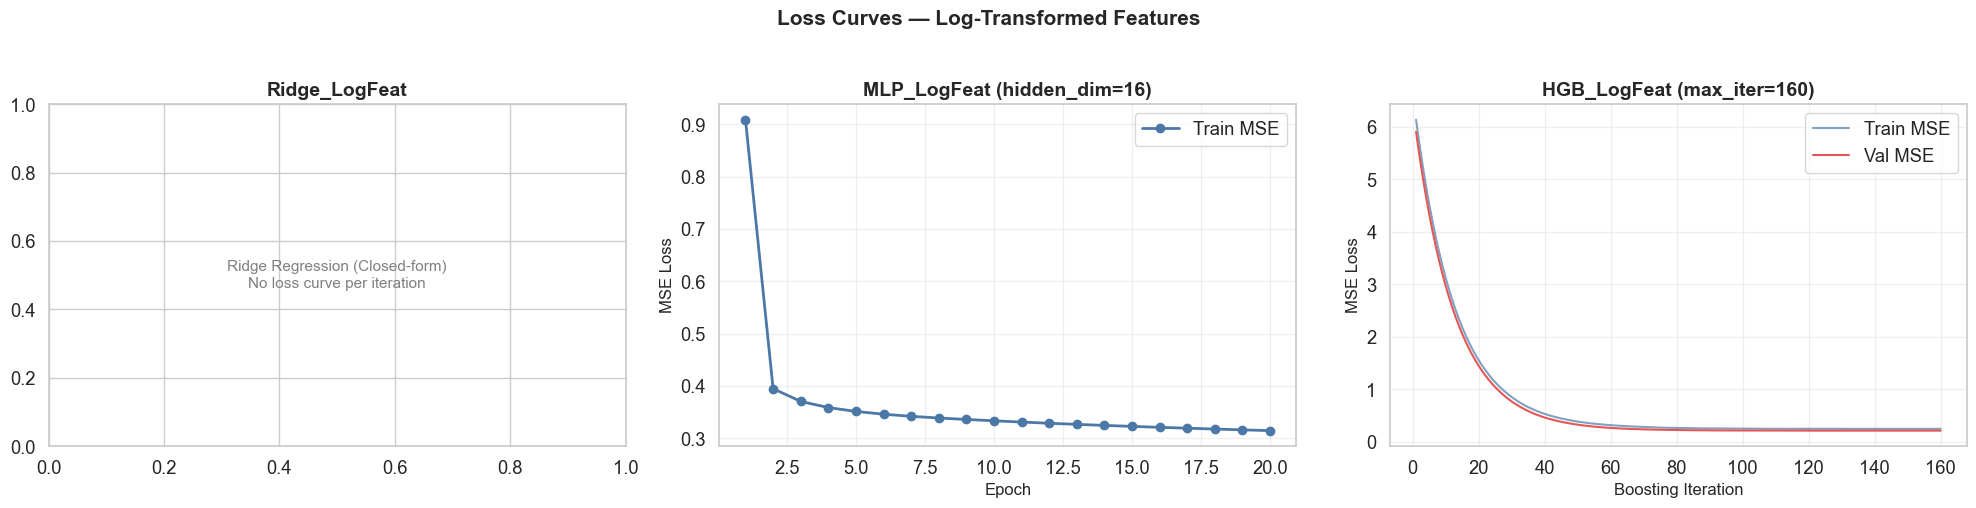
\includegraphics[width=\textwidth]{figures/lab02/eda_015.png}
  \caption{Top states by revenue}
\end{figure}\
\vspace{4pt}
\begin{figure}[H]
  \centering
  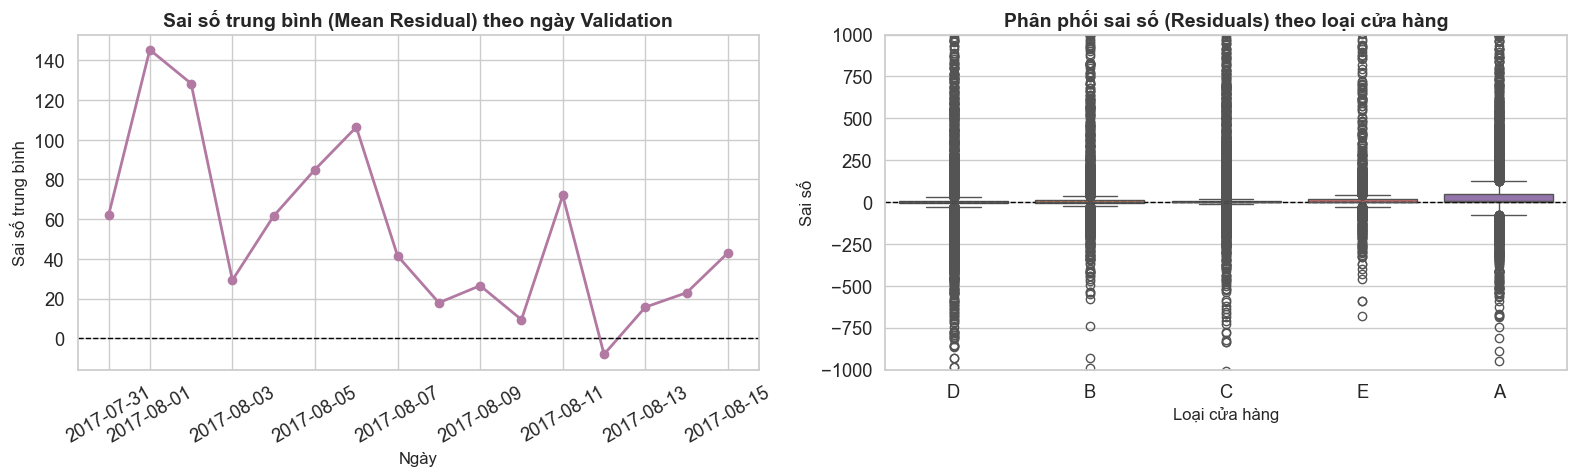
\includegraphics[width=\textwidth]{figures/lab02/eda_017.png}
  \caption{Top products by revenue}
\end{figure}
\begin{figure}[H]
  \centering
  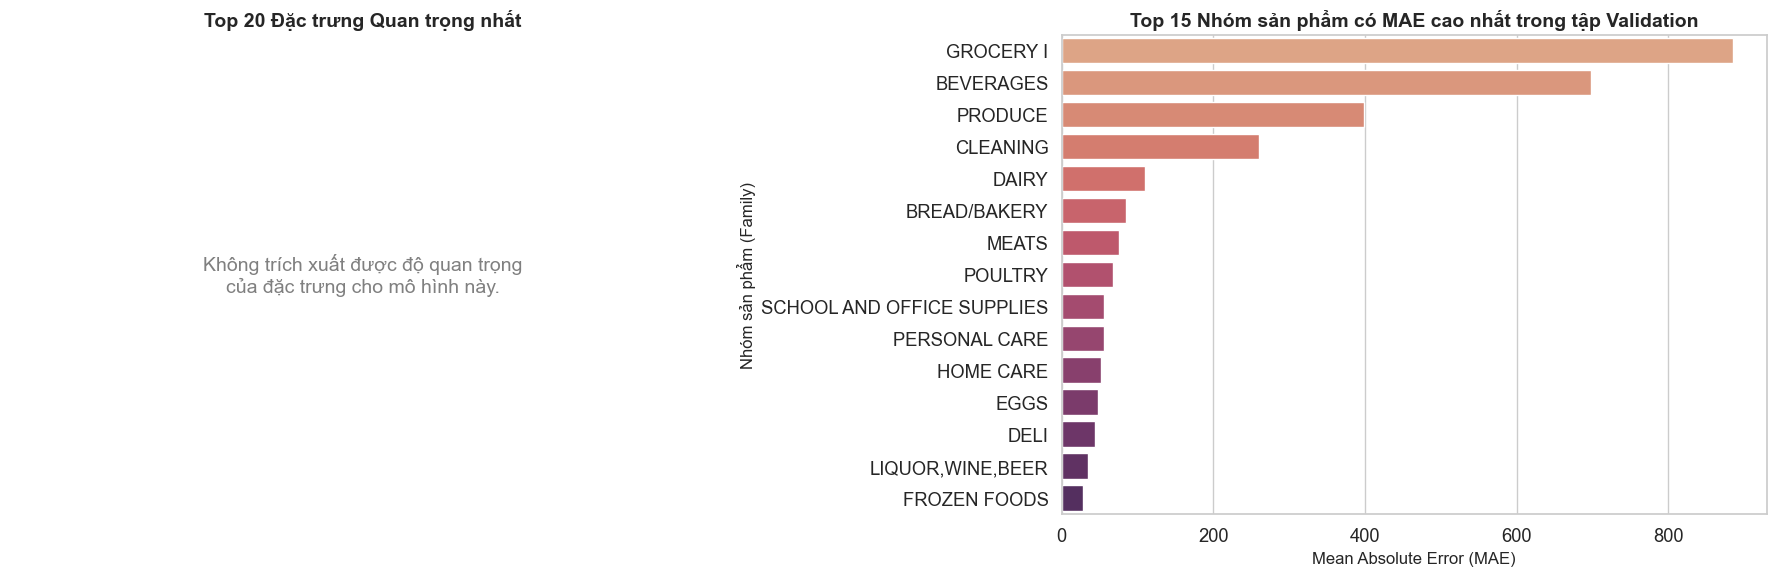
\includegraphics[width=\textwidth]{figures/lab02/eda_018.png}
  \caption{Revenue by category detail}
\end{figure}
\end{figure}

\begin{figure}[H]\centering
\begin{figure}[H]
  \centering
  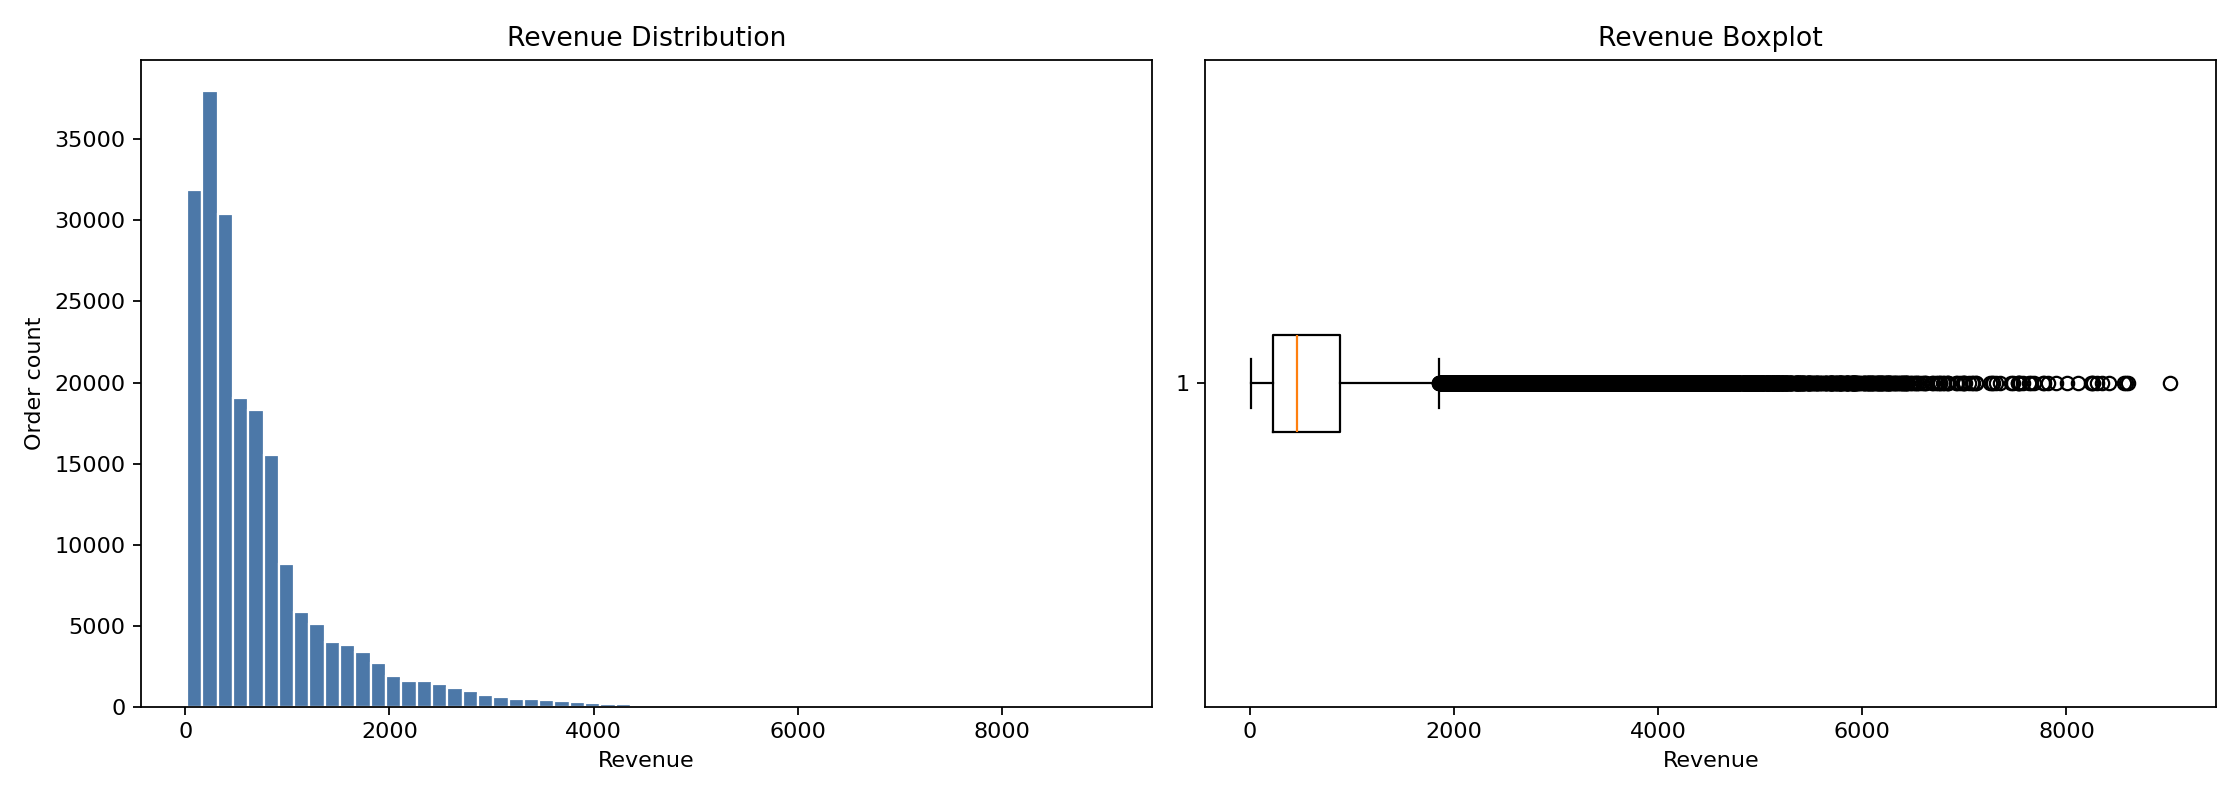
\includegraphics[width=\textwidth]{figures/lab02/notebook_revenue_distribution_boxplot.png}
  \caption{Revenue distribution boxplot}
\end{figure}
\begin{figure}[H]
  \centering
  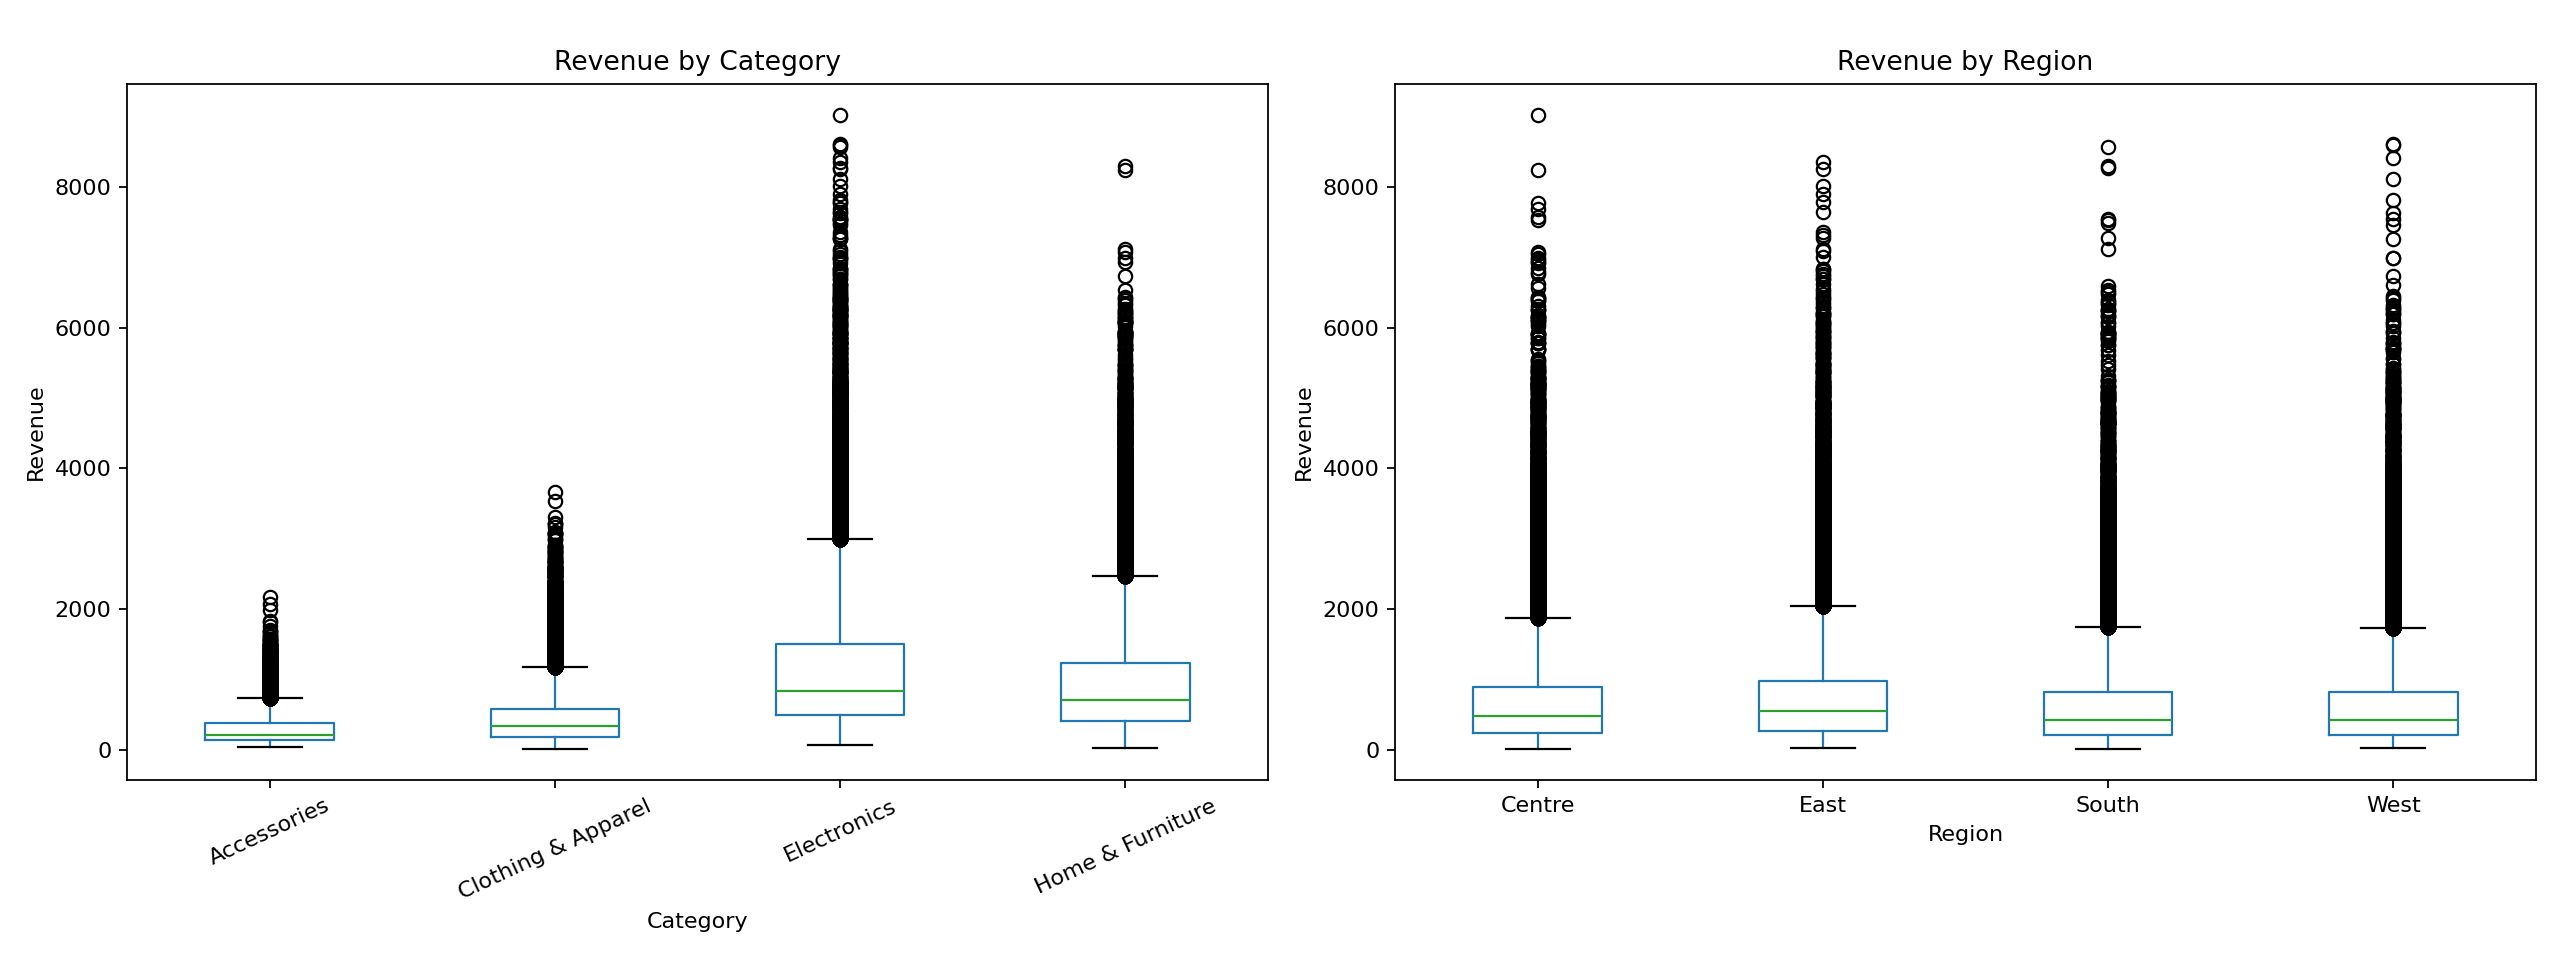
\includegraphics[width=\textwidth]{figures/lab02/notebook_revenue_boxplot_by_segments.png}
  \caption{Revenue by segments}
\end{figure}\
\vspace{4pt}
\begin{figure}[H]
  \centering
  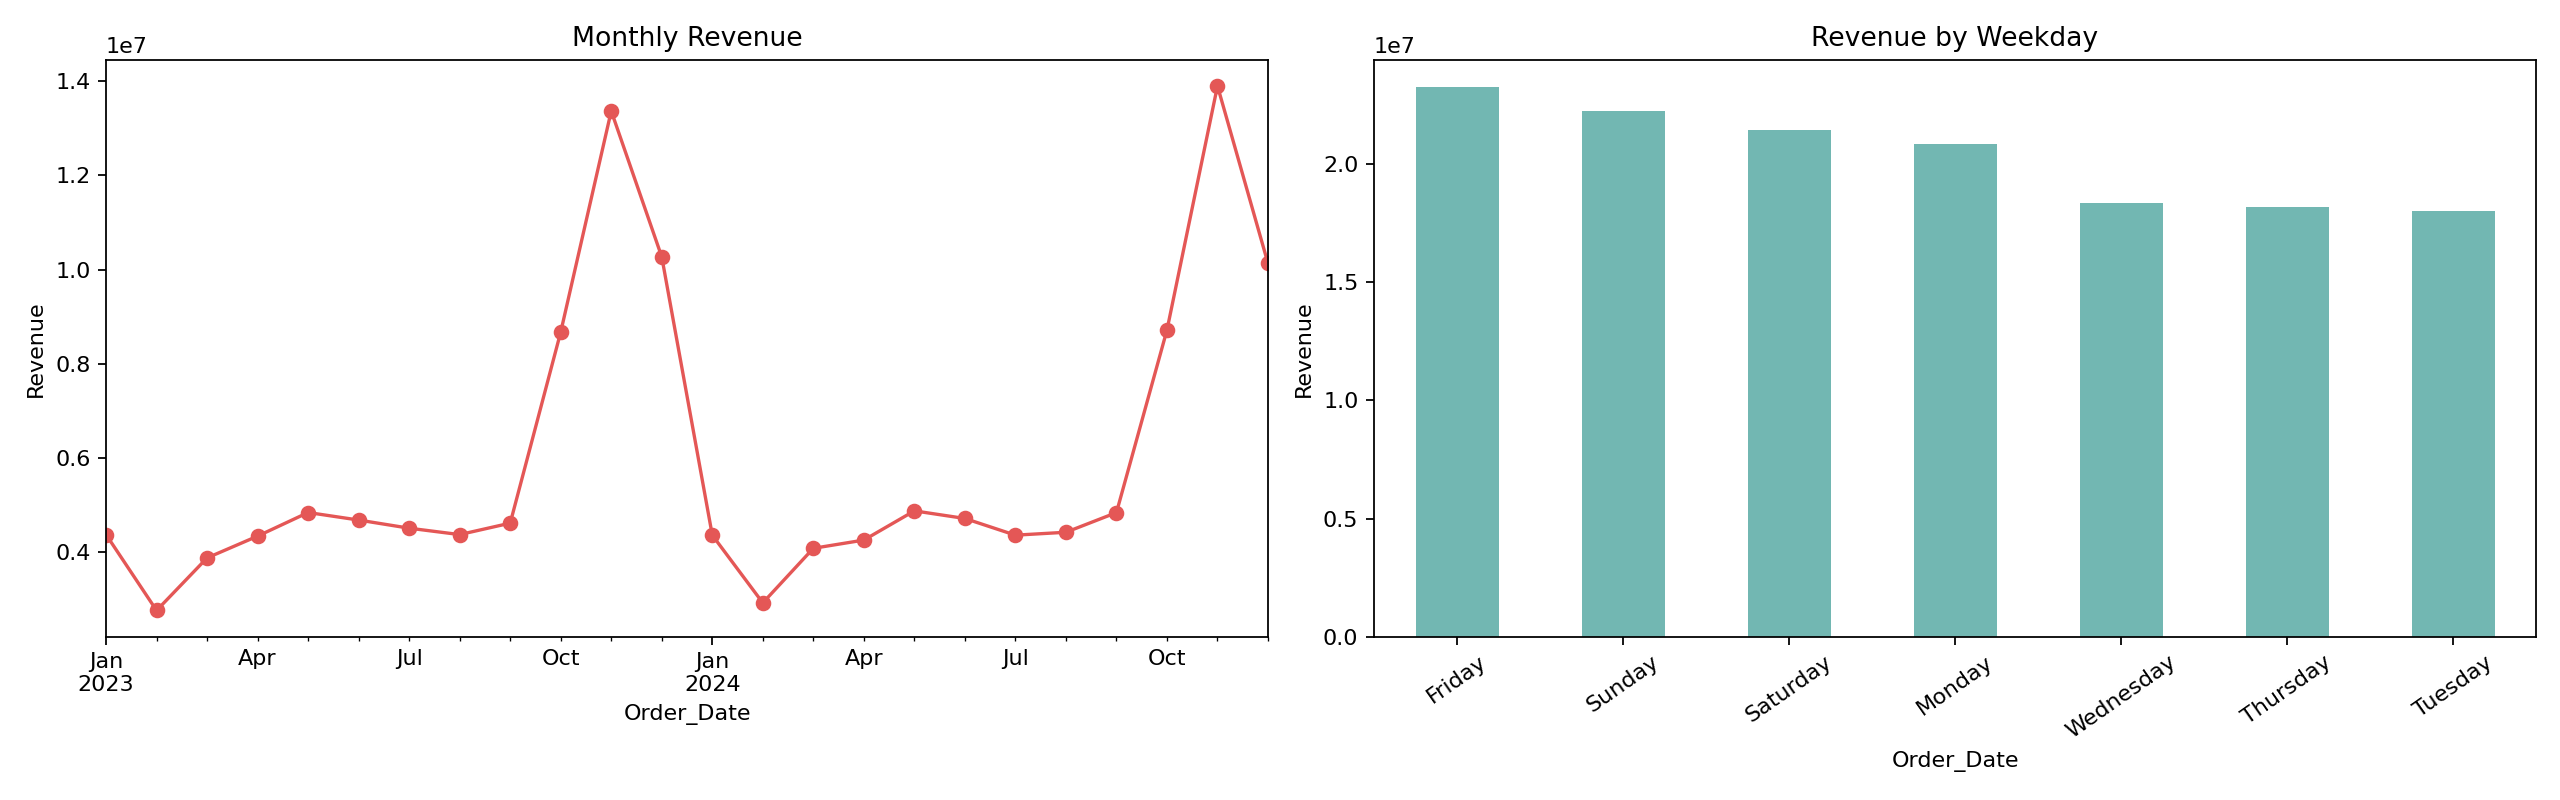
\includegraphics[width=\textwidth]{figures/lab02/notebook_time_eda.png}
  \caption{Time-series EDA patterns}
\end{figure}
\begin{figure}[H]
  \centering
  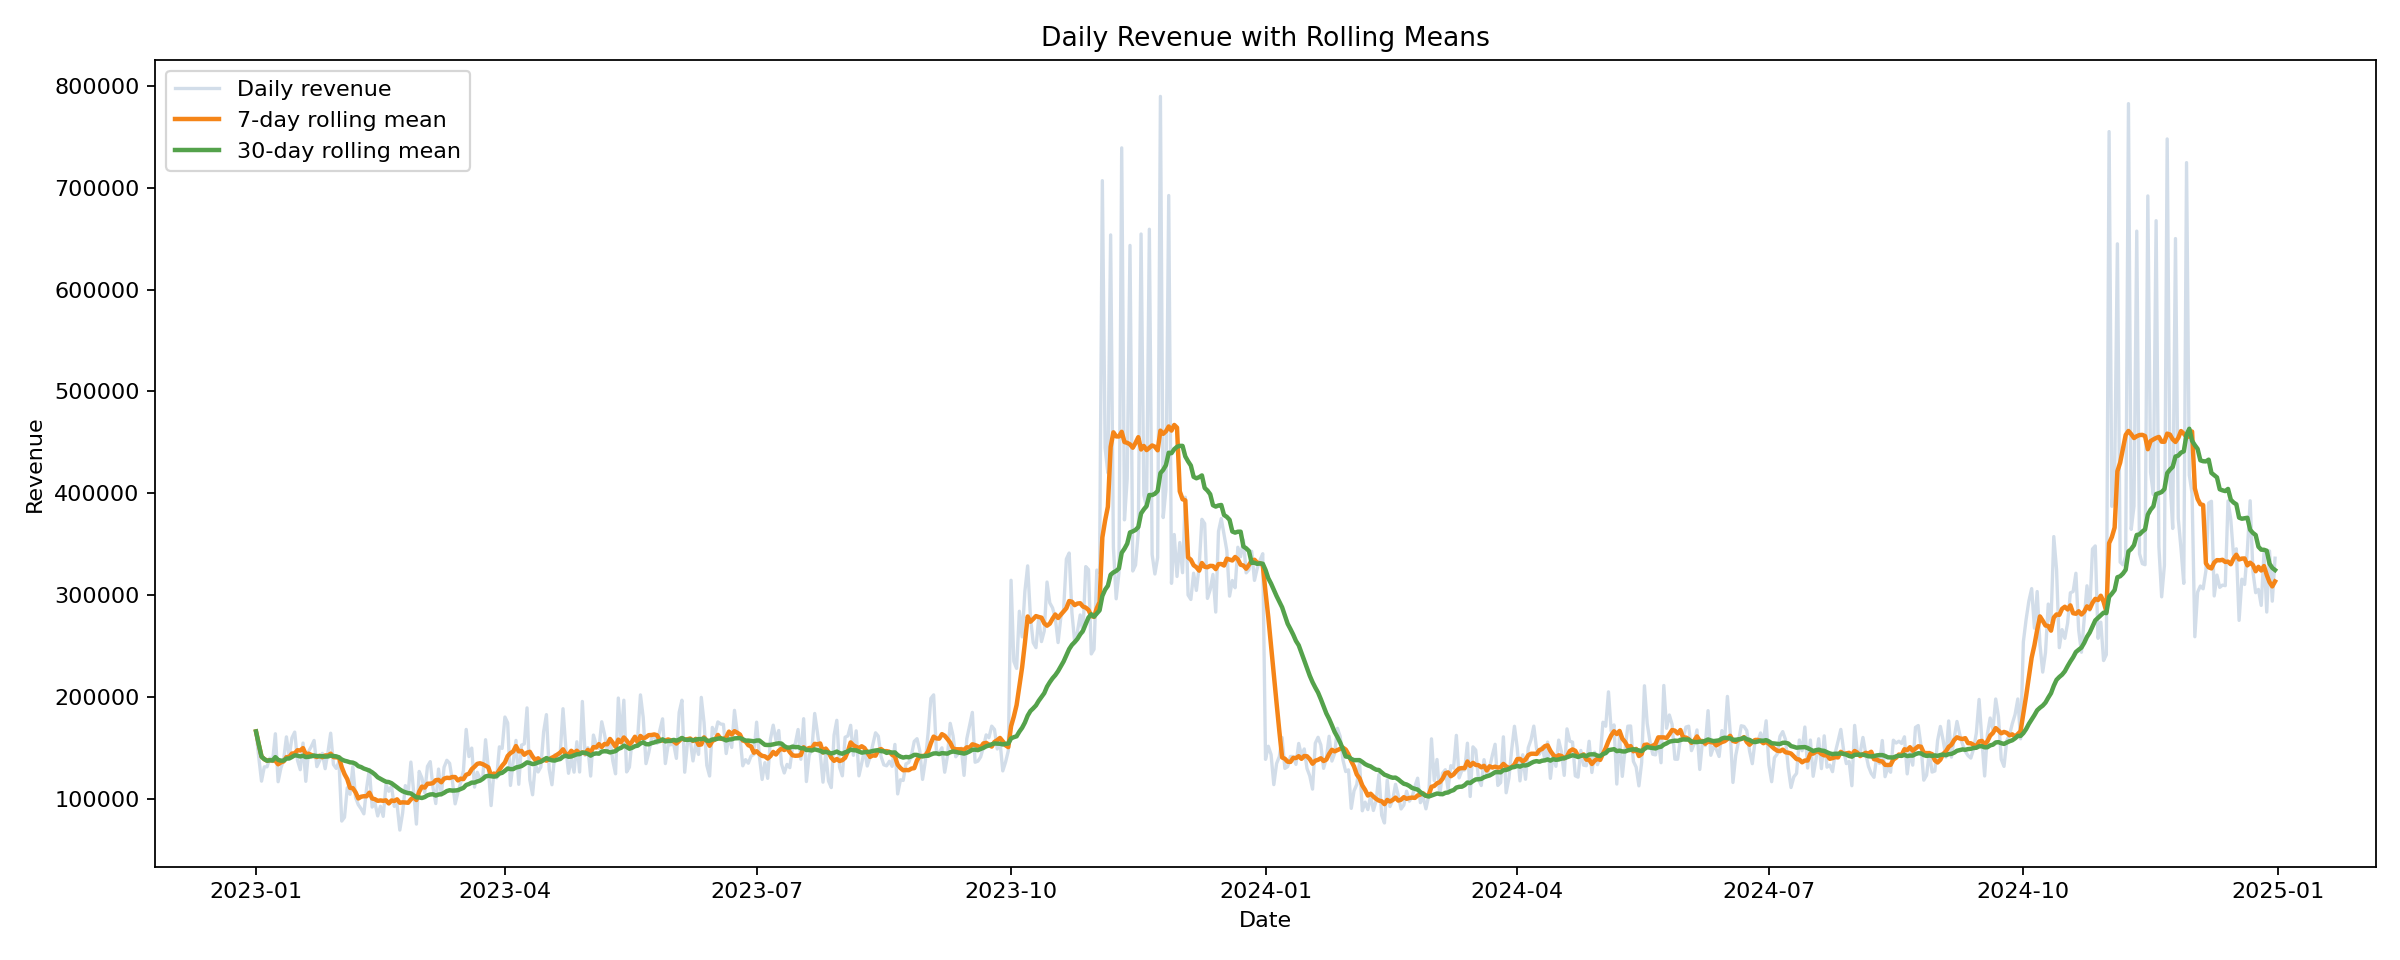
\includegraphics[width=\textwidth]{figures/lab02/notebook_daily_revenue_rolling_mean.png}
  \caption{Daily revenue rolling mean}
\end{figure}
\end{figure}

\begin{figure}[H]\centering
\begin{figure}[H]
  \centering
  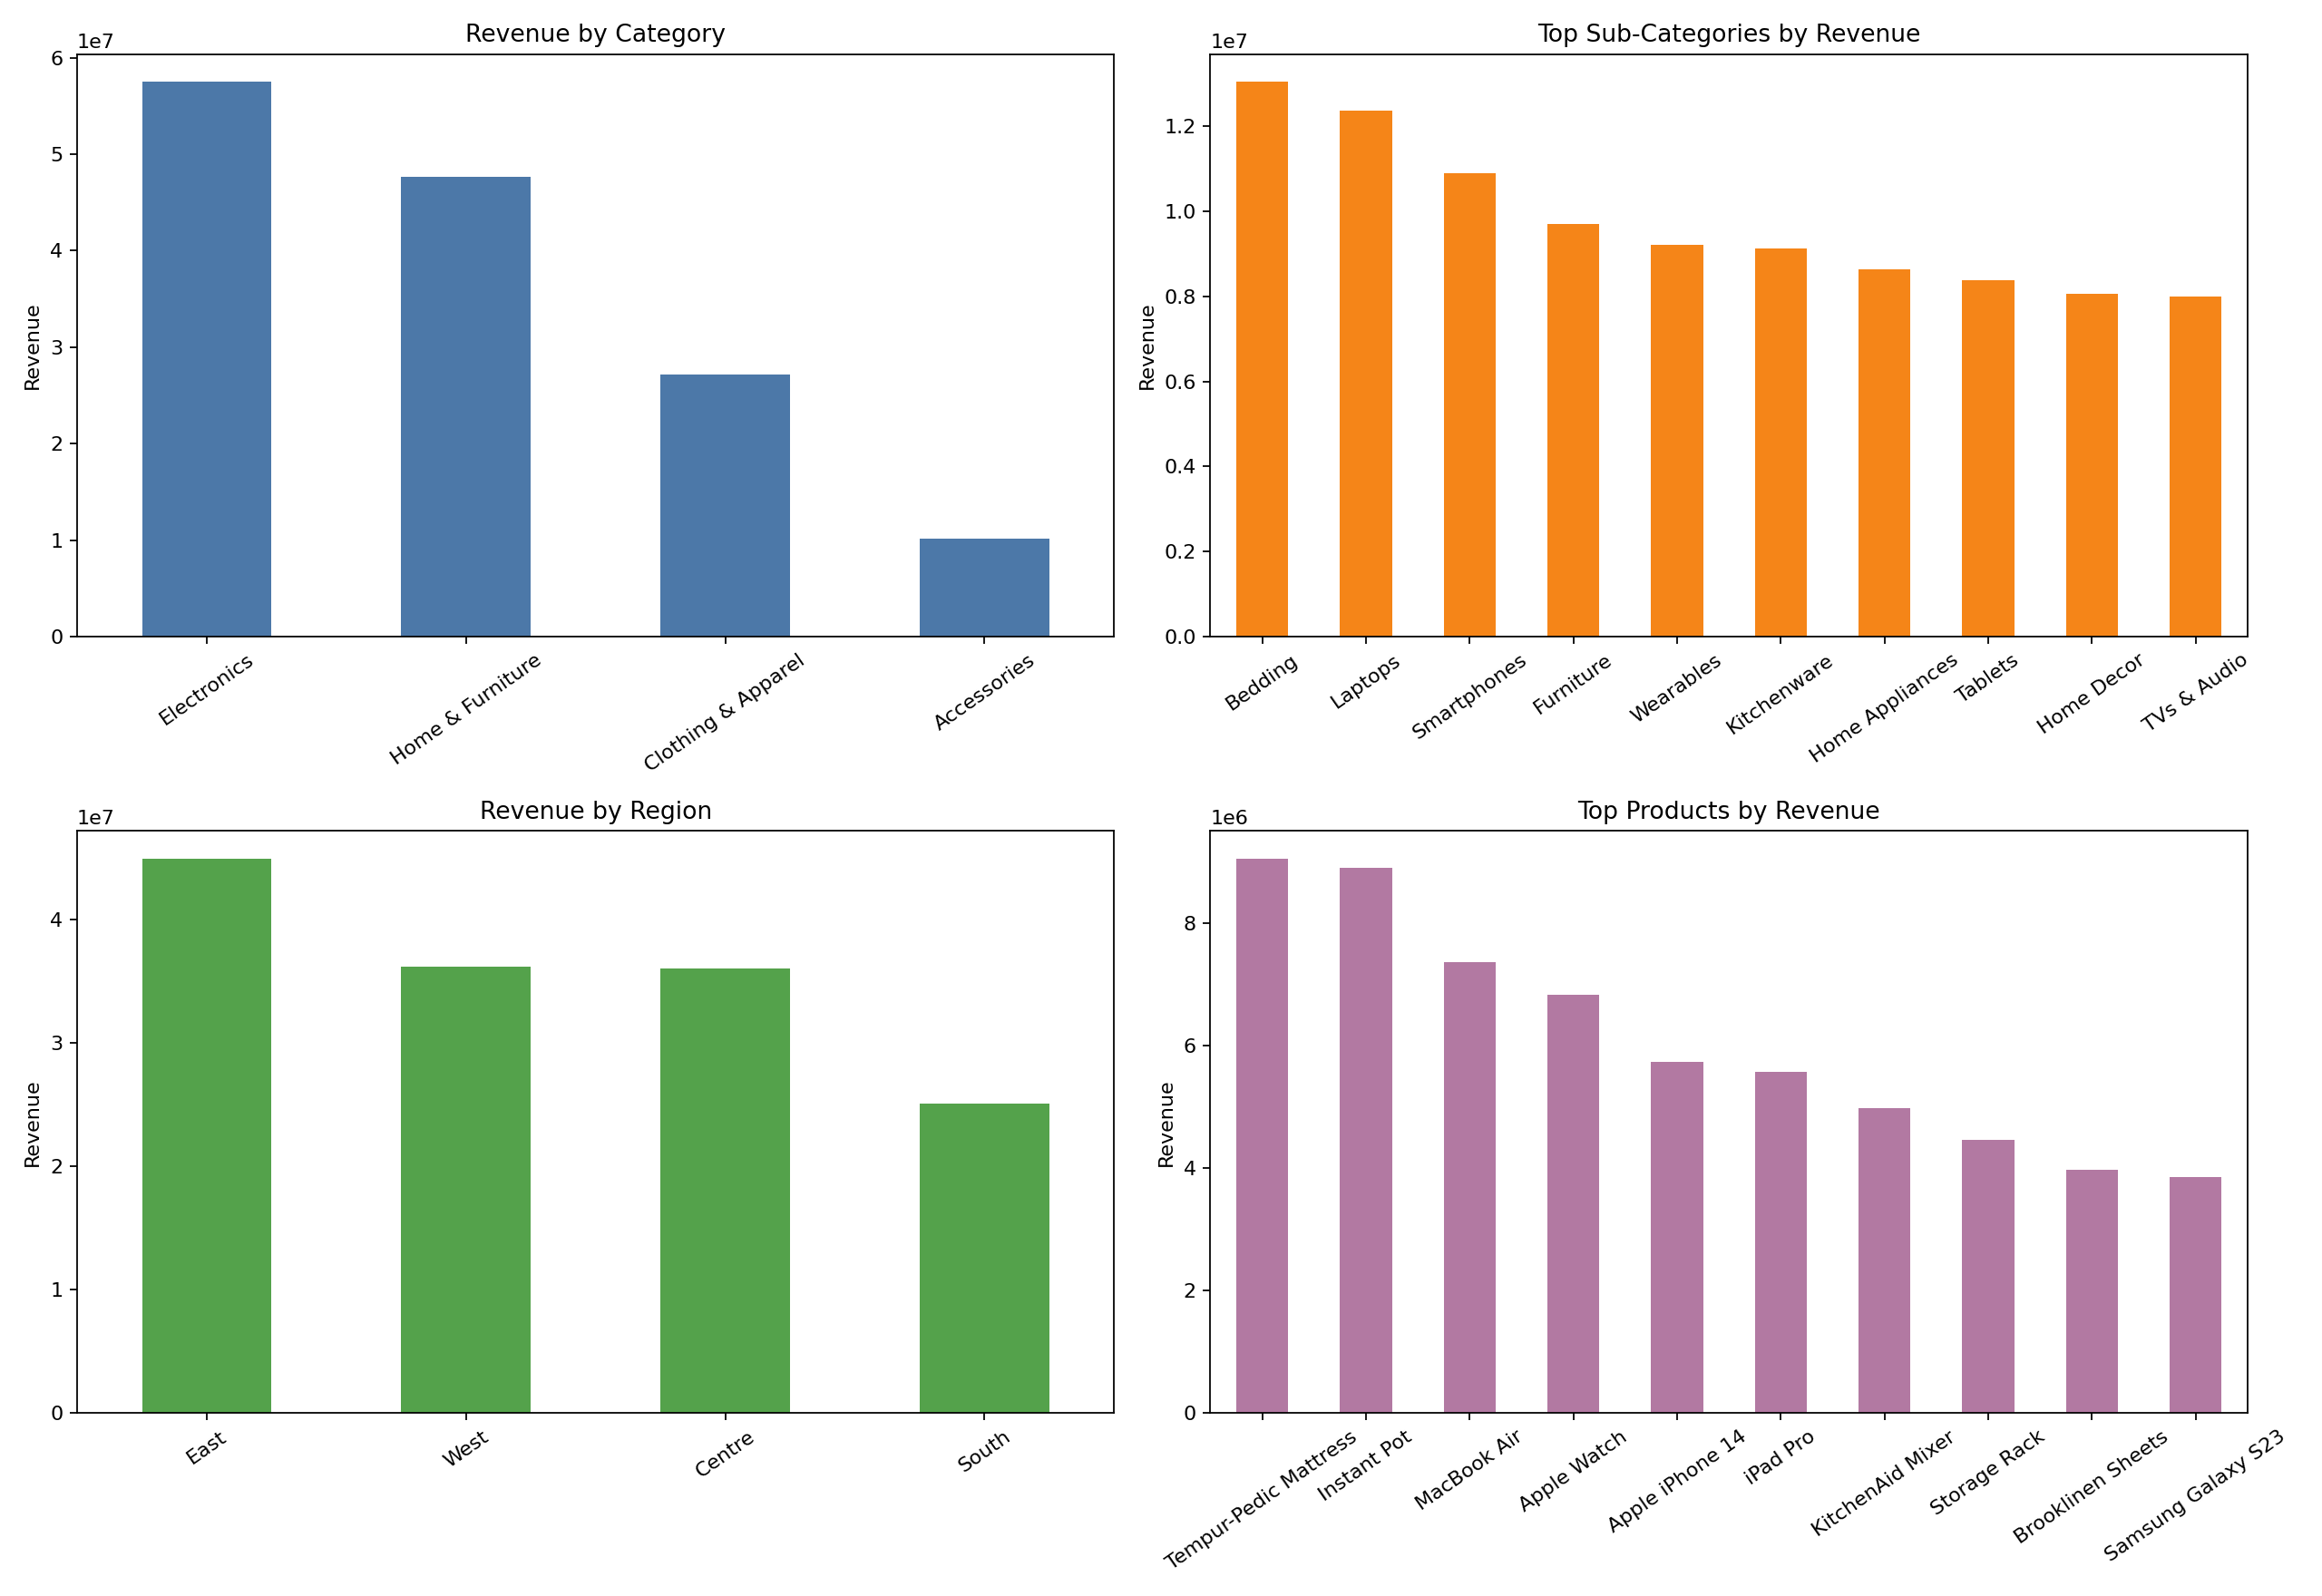
\includegraphics[width=\textwidth]{figures/lab02/notebook_product_geography_eda.png}
  \caption{Product geography analysis}
\end{figure}
\begin{figure}[H]
  \centering
  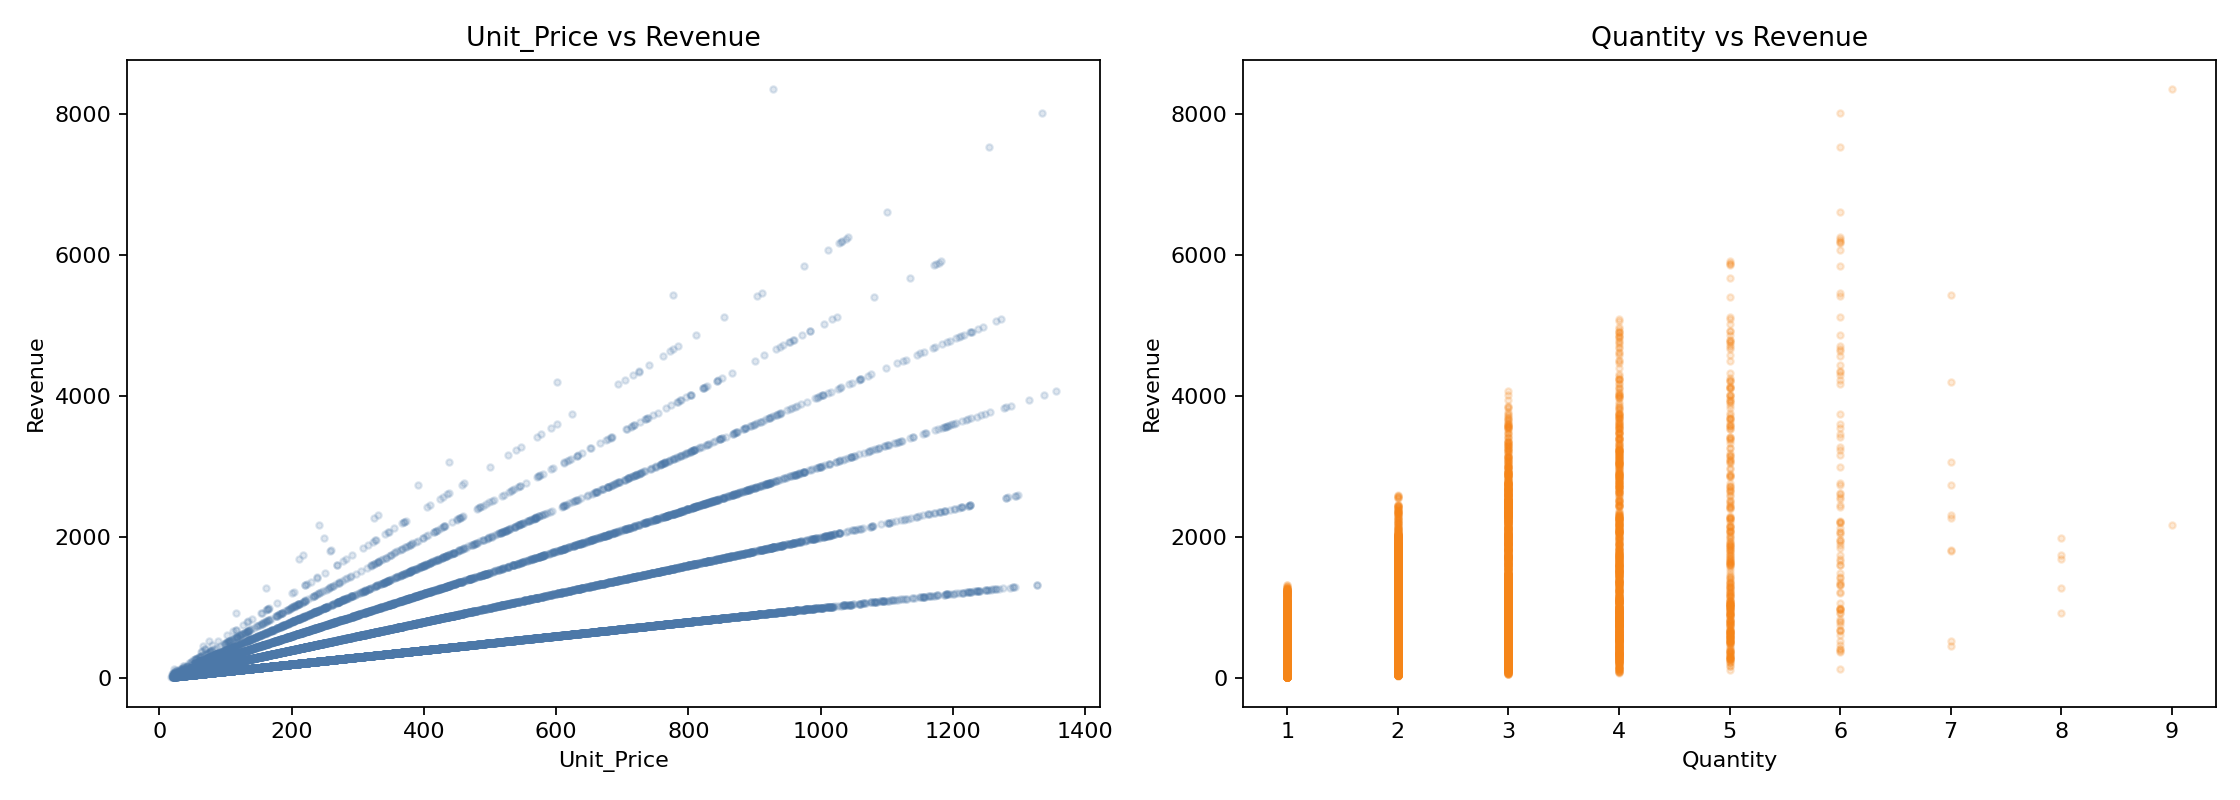
\includegraphics[width=\textwidth]{figures/lab02/notebook_relationship_eda.png}
  \caption{Feature relationship analysis}
\end{figure}\
\vspace{4pt}
\begin{figure}[H]
  \centering
  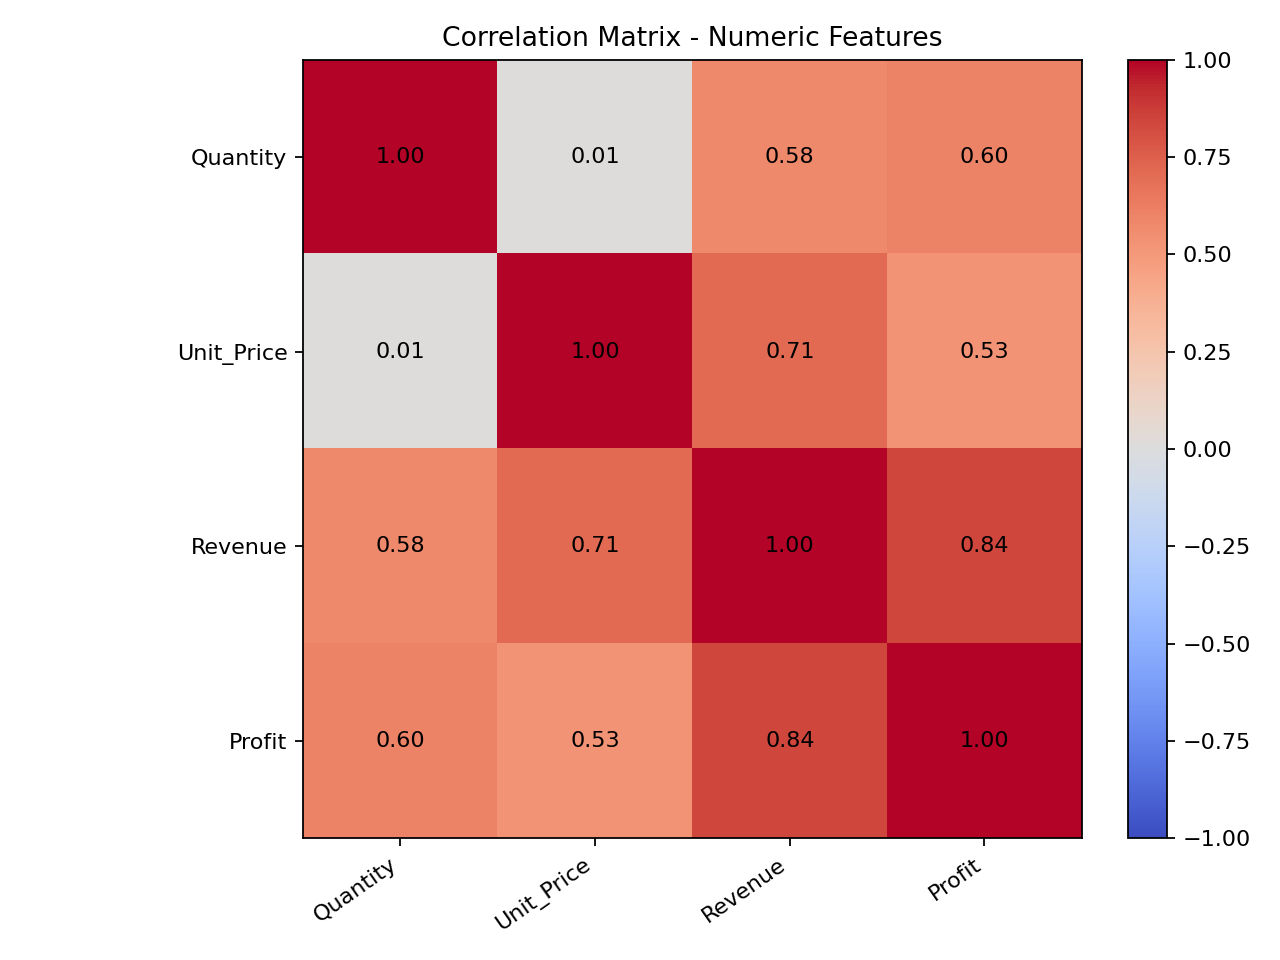
\includegraphics[width=\textwidth]{figures/lab02/notebook_numeric_correlation_heatmap.png}
  \caption{Numeric correlation heatmap}
\end{figure}
\begin{figure}[H]
  \centering
  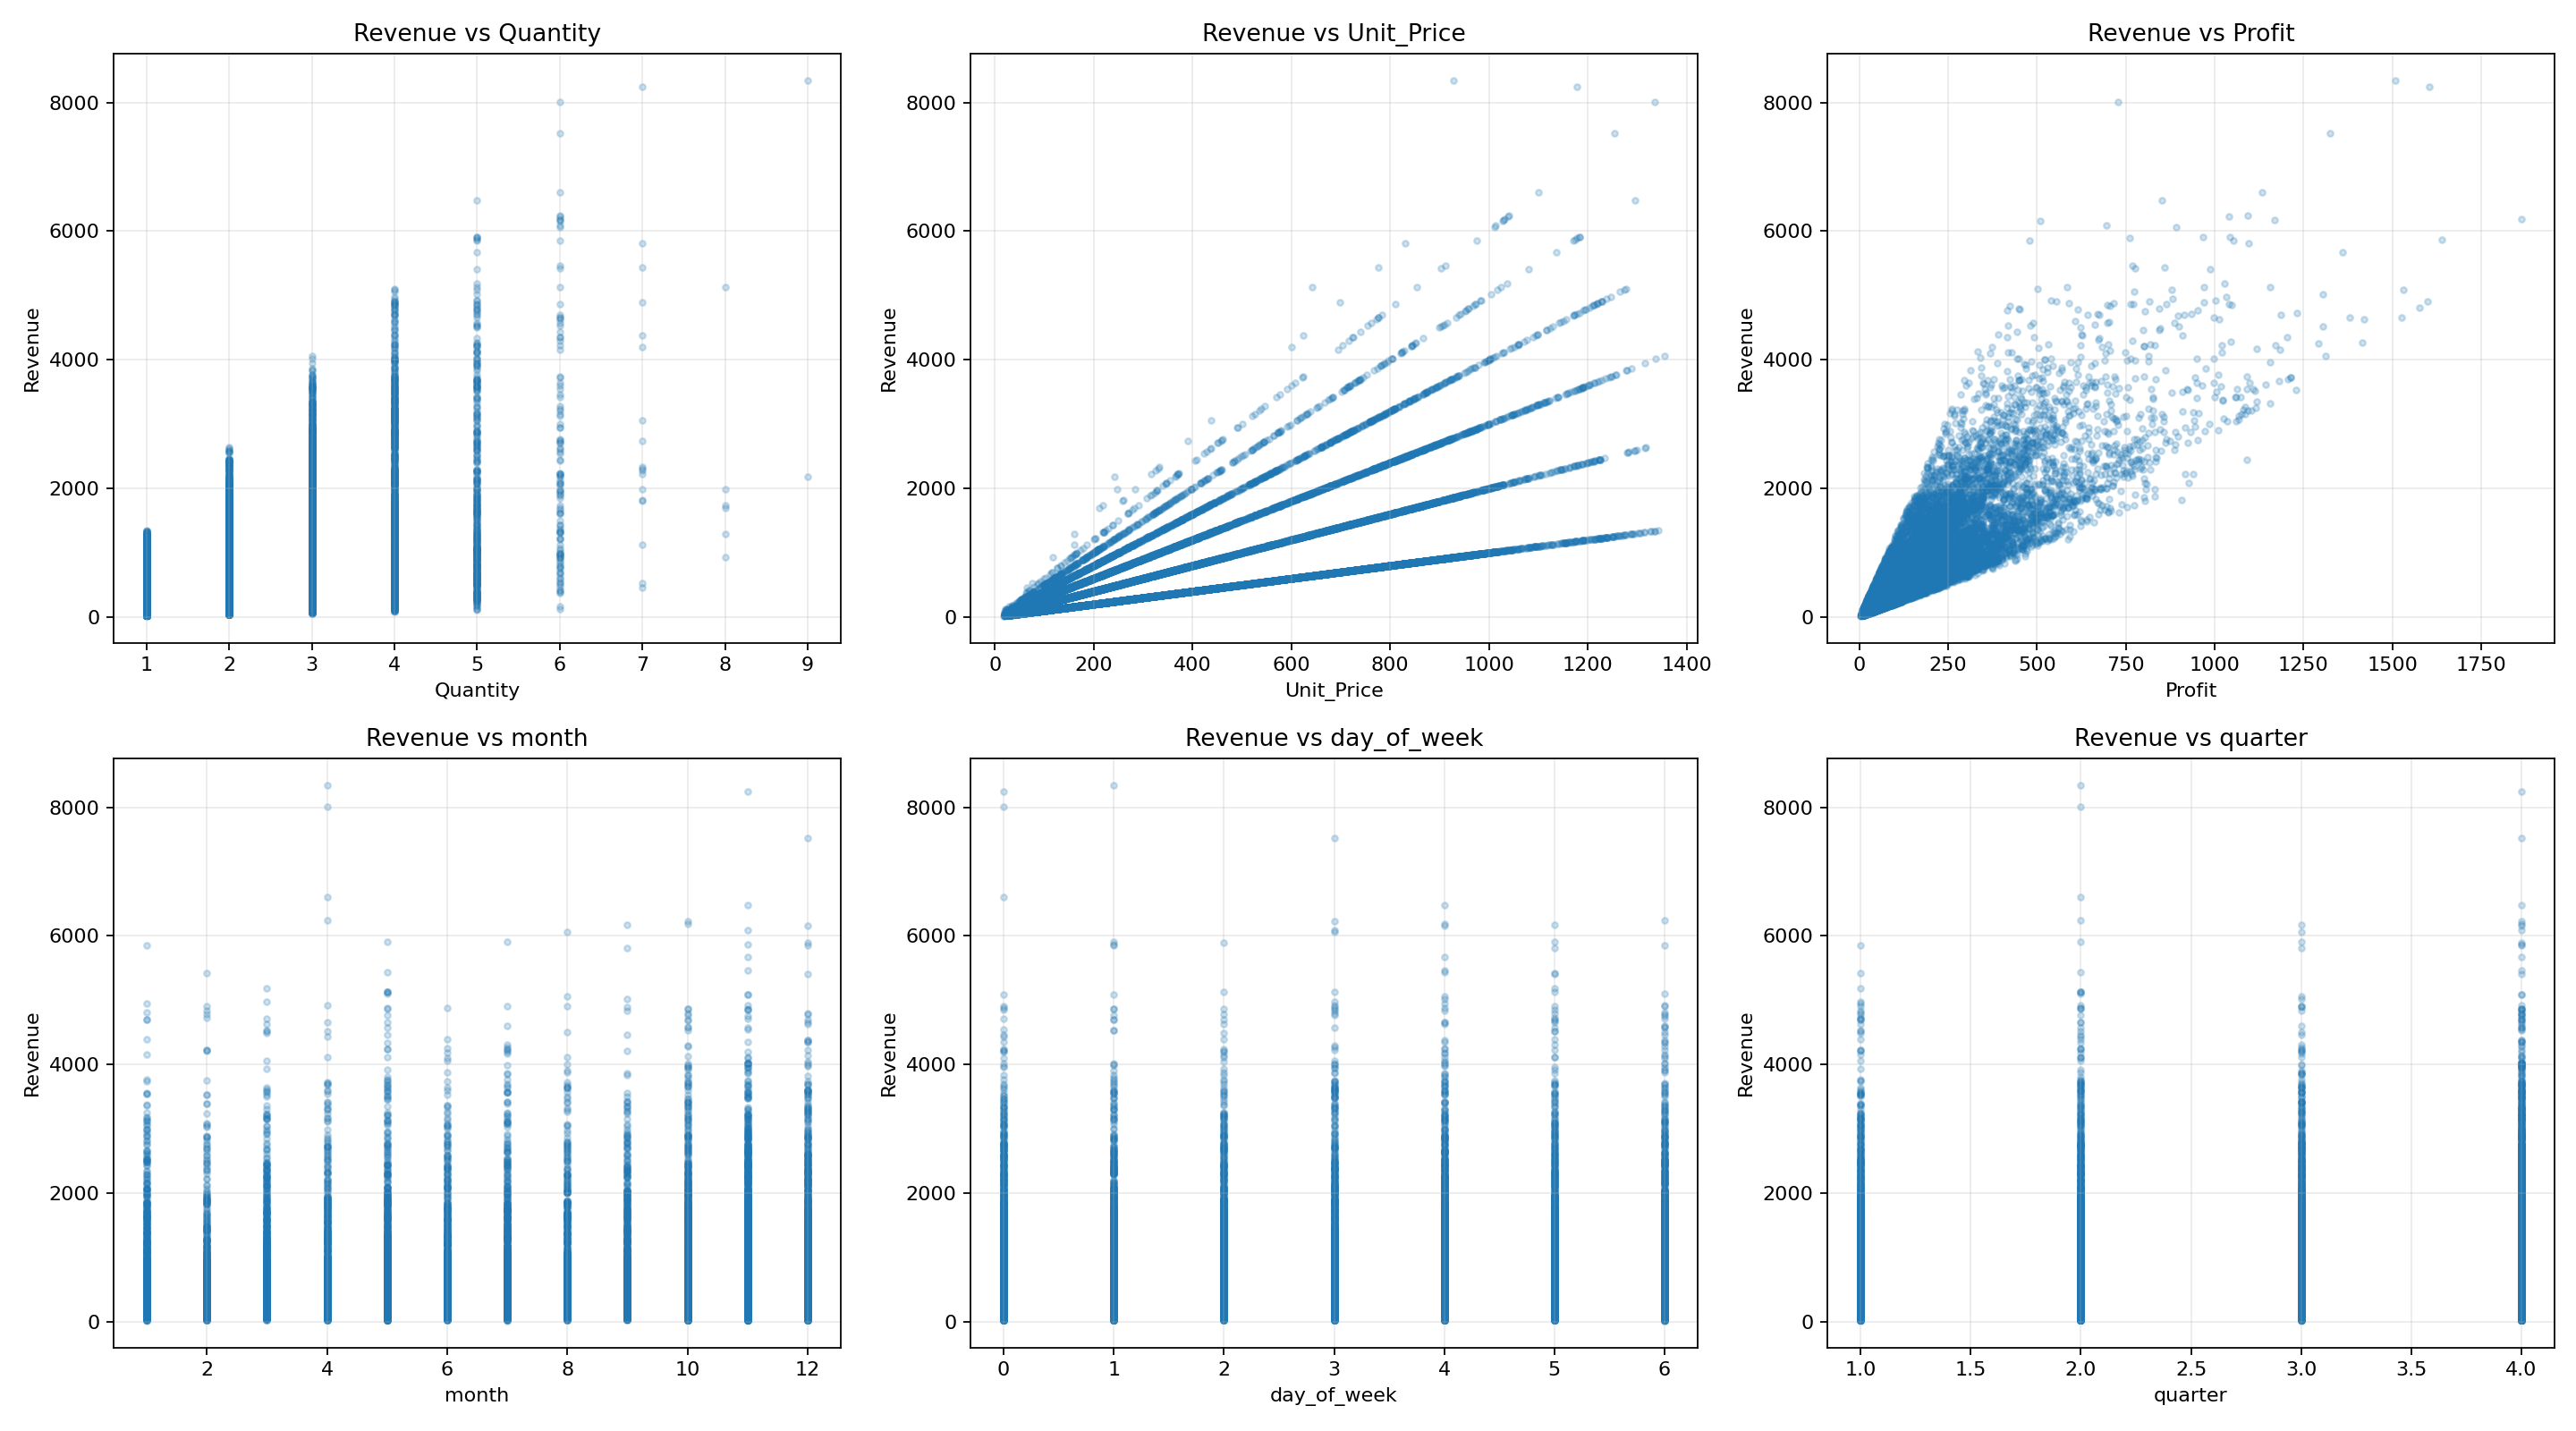
\includegraphics[width=\textwidth]{figures/lab02/notebook_scatter_grid_features_vs_revenue.png}
  \caption{Feature scatter grid vs. revenue}
\end{figure}
\end{figure}

\begin{figure}[H]\centering
\begin{figure}[H]
  \centering
  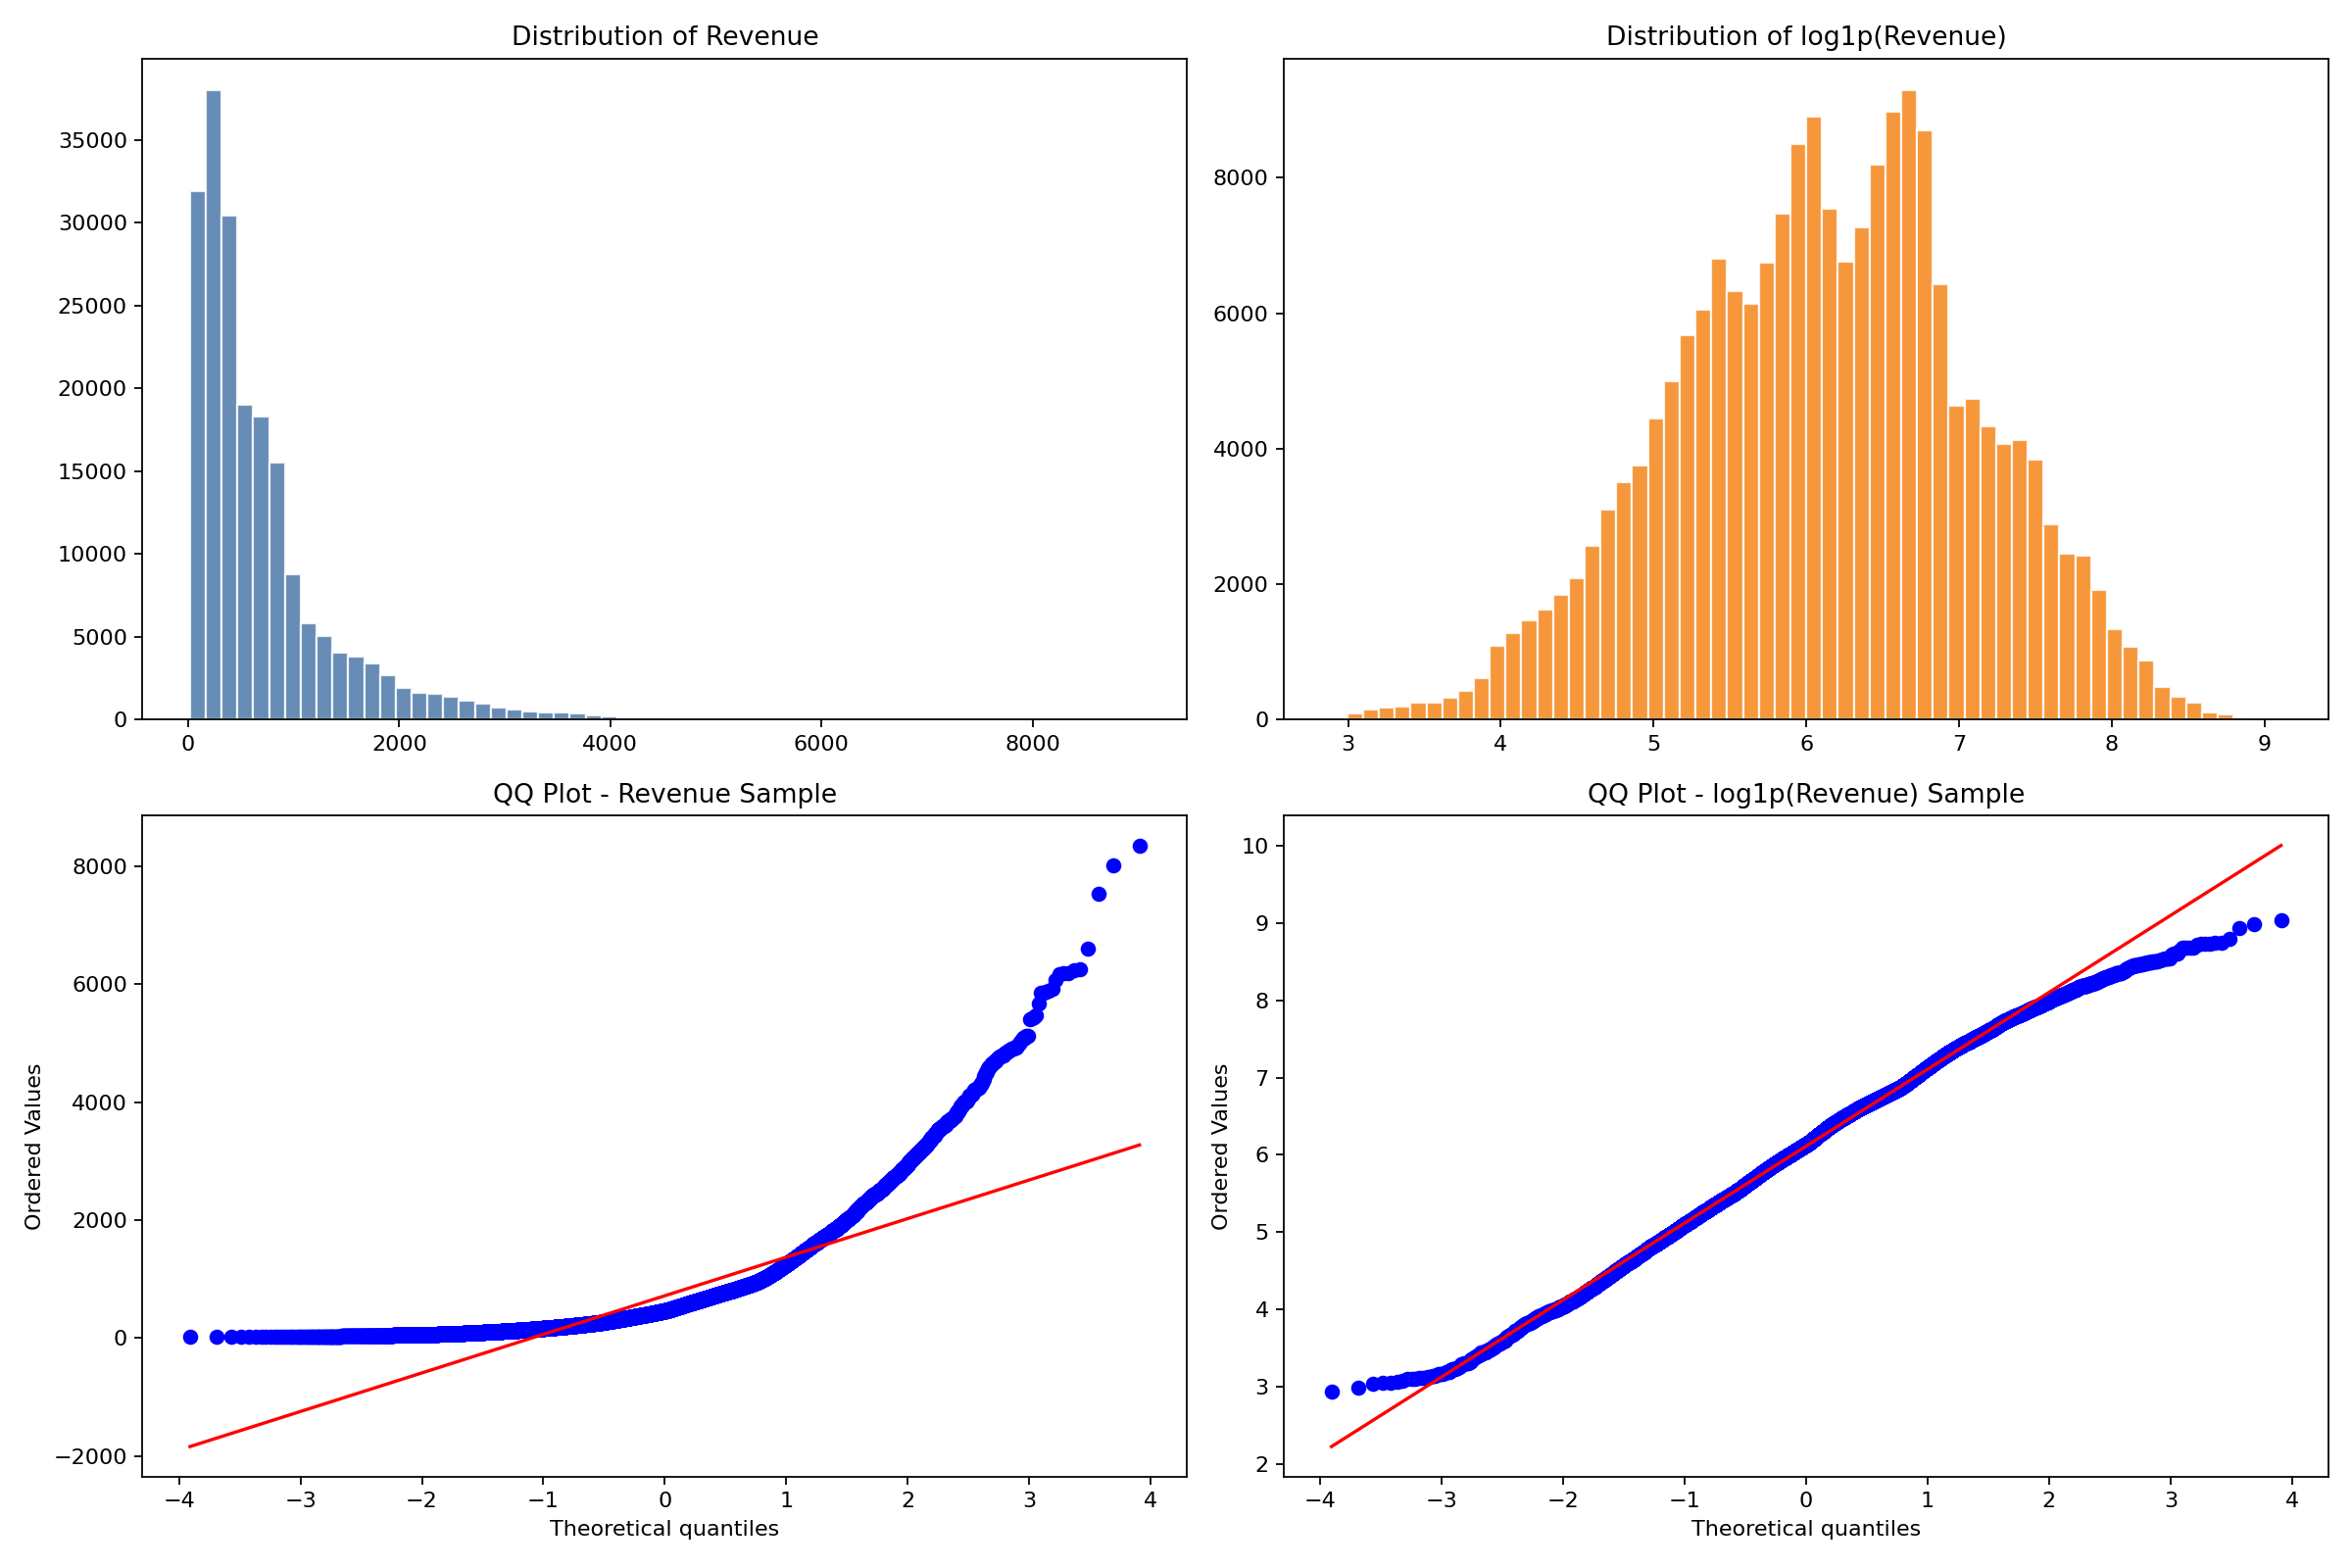
\includegraphics[width=\textwidth]{figures/lab02/notebook_advanced_target_distribution.png}
  \caption{Advanced target distribution}
\end{figure}
\begin{figure}[H]
  \centering
  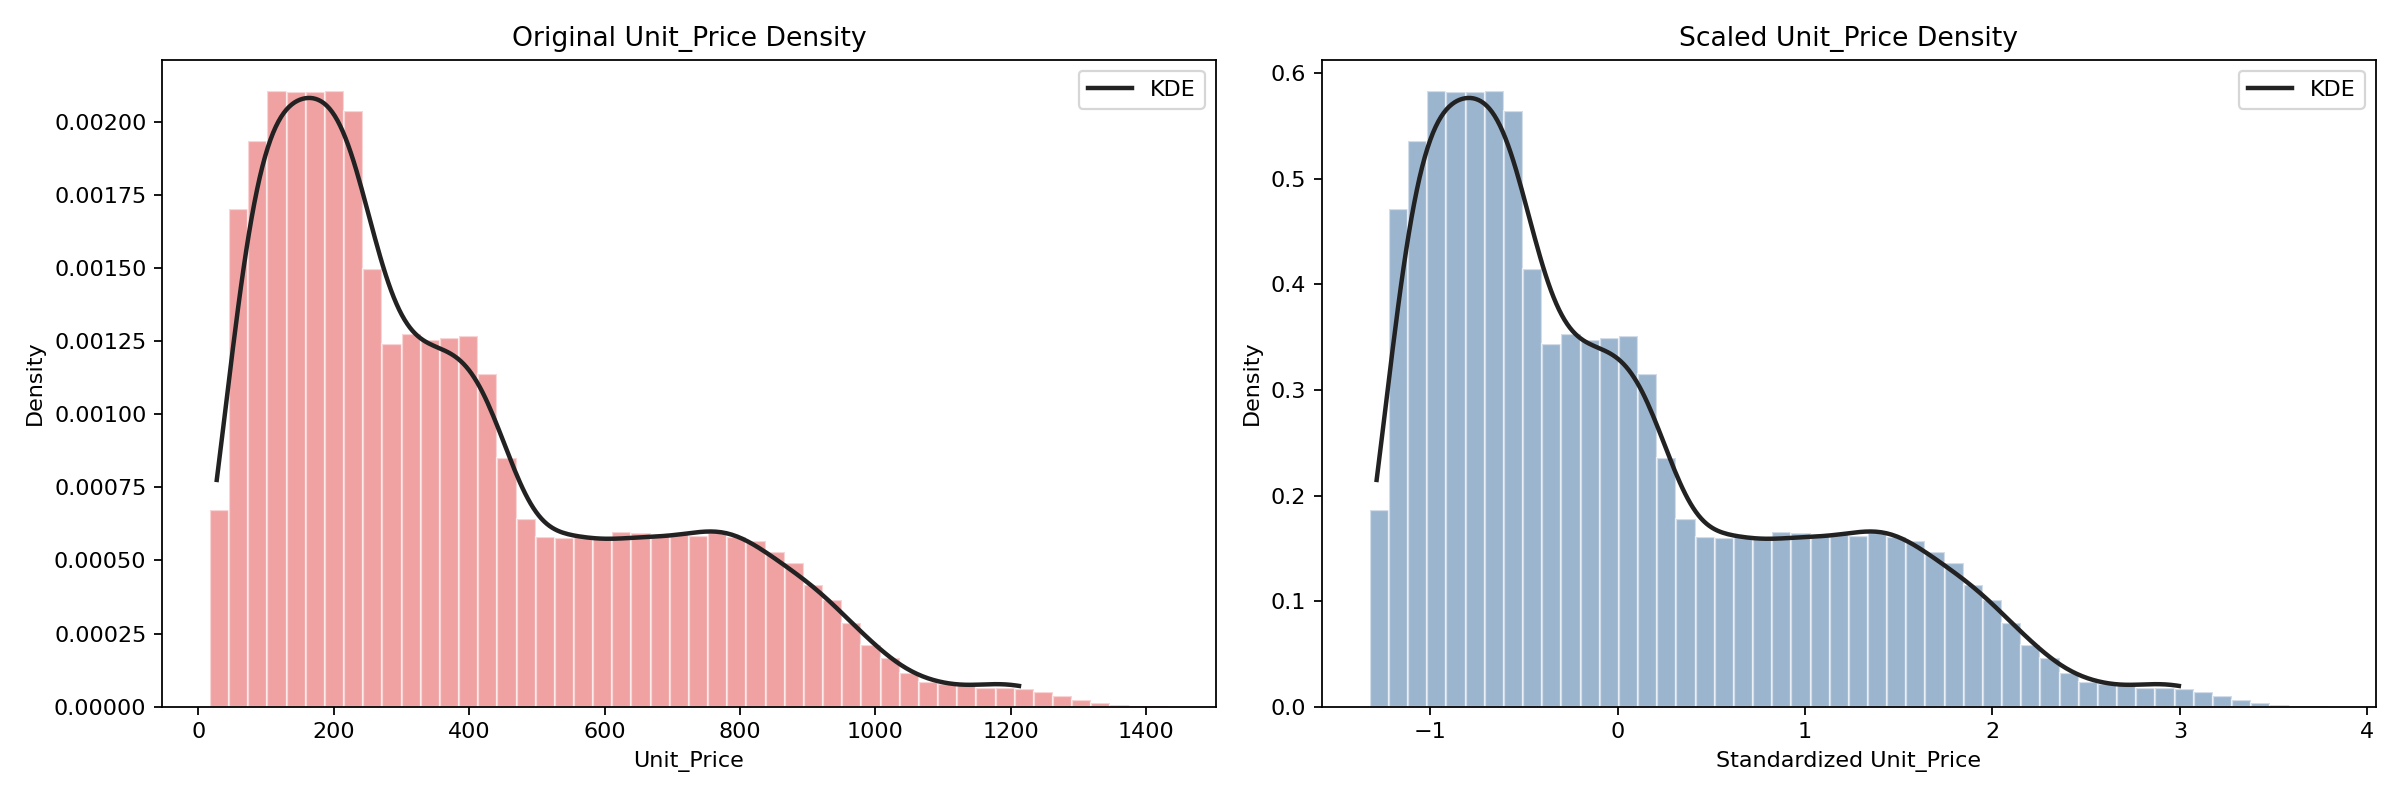
\includegraphics[width=\textwidth]{figures/lab02/notebook_density_original_vs_scaled.png}
  \caption{Density: original vs. scaled}
\end{figure}
\end{figure}

\subsection{Step 2.5 — Data Cleaning}
Duplicate rows are checked and dropped across all six tables. Oil price gaps are filled inside the feature-building function with \texttt{ffill()}$\rightarrow$\texttt{bfill()}. The standardization strategy depends on model family:

\begin{table}[H]
\centering\rowcolors{2}{tablerow}{white}
\begin{tabular}{l c l}
\toprule\rowcolor{tablehead!80}\color{white}\textbf{Model} &\color{white}\textbf{Scaling?} &\color{white}\textbf{Reason}\\
\midrule
Ridge & Yes (StandardScaler) & L2 penalty treats all features equally; unscaled features get unfair regularization\\
MLP & Yes (StandardScaler) & SGD converges faster when features share a similar scale\\
HistGradientBoosting & No & Tree splits depend on rank order, not absolute values\\
\bottomrule
\end{tabular}
\caption{Scaling strategy per model family}
\end{table}

\subsection{Step 3 — Feature Engineering}

Four feature groups are engineered, each answering a distinct question:

\begin{table}[H]
\centering\rowcolors{2}{tablerow}{white}
\begin{tabular}{l L{2.5cm} L{5.5cm} L{4cm}}
\toprule\rowcolor{tablehead!80}\color{white}\textbf{Group} &\color{white}\textbf{Count} &\color{white}\textbf{Features} &\color{white}\textbf{Question}\\
\midrule
Calendar & 5 & \texttt{dayofweek}, \texttt{month}, \texttt{year}, \texttt{dayofmonth}, \texttt{is\_weekend} & What day is today?\\
Store & 6 & \texttt{store\_nbr}, \texttt{family}, \texttt{city}, \texttt{state}, \texttt{type}, \texttt{cluster} & What kind of store?\\
External & 3 & \texttt{dcoilwtico}, \texttt{is\_holiday}, \texttt{holiday\_count} & What's special today?\\
Time-series & 6 & \texttt{lag\_16}, \texttt{lag\_28}, \texttt{lag\_364}, rolling means (7/28/56 day, shifted 16) & What were past sales?\\
\bottomrule
\end{tabular}
\caption{Complete feature set: 20 features in 4 groups}
\end{table}

\textbf{The shift-16 mechanism:} The forecast horizon is 16 days. On day 1 of the horizon, the most recent known sale is at $t-16$. Every lag/rolling feature is shifted by 16 days:

\begin{pythoncode}[caption={Lag and rolling features with shift-16 guard}]
def add_lag_features(frame):
    out = frame.sort_values(["store_nbr", "family", "date"]).copy()
    grouped_sales = out.groupby(["store_nbr", "family"])["sales"]
    for lag in [16, 28, 364]:
        out[f"lag_{lag}"] = grouped_sales.shift(lag)
    out["rolling_mean_7_shift16"] = grouped_sales.transform(
        lambda s: s.shift(16).rolling(7, min_periods=1).mean()
    )
    out["rolling_mean_28_shift16"] = grouped_sales.transform(
        lambda s: s.shift(16).rolling(28, min_periods=1).mean()
    )
    out["rolling_mean_56_shift16"] = grouped_sales.transform(
        lambda s: s.shift(16).rolling(56, min_periods=1).mean()
    )
    return out
\end{pythoncode}

The key insight: the \texttt{.shift(16)} on the raw sales column before applying \texttt{.rolling()} is what makes this production-ready. Without it, a `lag\_1' feature would leak tomorrow's sales at prediction time.

\subsection{Step 4 — Time-Based Train/Validation Split}

Unlike standard machine learning where random shuffling is acceptable, time-series data must respect chronological order. The split:

\begin{table}[H]
\centering\rowcolors{2}{tablerow}{white}
\begin{tabular}{l L{4cm} c}
\toprule\rowcolor{tablehead!80}\color{white}\textbf{Set} &\color{white}\textbf{Date Range} &\color{white}\textbf{Rows}\\
\midrule
Train (\texttt{fit\_df}) & 365 days before validation start & $\sim$650k\\
Validation (\texttt{valid\_df}) & Last 16 days & $\sim$28k\\
\bottomrule
\end{tabular}
\caption{Time-based split — no random shuffling}
\end{table}

Only 365 days are used: (1) the full 5-year dataset is memory/compute intensive; (2) old sales patterns may be stale; (3) max lag is 364, so 365 days provides full coverage. A post-engineering correlation matrix confirms: \texttt{lag\_16} and rolling means have the highest correlation with sales ($>0.6$); \texttt{onpromotion} is moderate (0.2–0.4); \texttt{dcoilwtico} is weak ($<0.2$).

\subsection{Step 5 — Metrics and Preprocessing Pipelines}

\subsubsection{Why RMSLE over RMSE?}
Two stores: Store A sells 100 units, predicted 110 (error=10, 10\% off); Store B sells 10 units, predicted 20 (error=10, 100\% off). RMSE treats both as equal errors. RMSLE penalizes \textbf{relative} error — appropriate for retail where a 10-unit miss at a small store is proportionally much larger.

\[
\text{RMSLE} = \sqrt{\frac{1}{n}\sum_{i=1}^{n}\left(\log(1+y_i) - \log(1+\hat{y}_i)\right)^2}
\]

\textbf{Two pipelines} are constructed:
\begin{enumerate}
  \item \textbf{One-hot pipeline} — \texttt{MedianImputer $\rightarrow$ StandardScaler / OneHotEncoder}. For Ridge and MLP (scale-sensitive).
  \item \textbf{Ordinal pipeline} — \texttt{MedianImputer / OrdinalEncoder}. For HistGradientBoosting (scale-invariant).
\end{enumerate}

Models train on $\log_{1p}(\texttt{sales})$; predictions are inverted with $\exp_{m1}$.

\subsection{Step 6 — Time-Series Baselines}

Four naive forecasts establish a floor — if a complex ML model cannot beat these, the features are too weak:

\begin{table}[H]
\centering\rowcolors{2}{tablerow}{white}
\begin{tabular}{l L{4cm} L{4.5cm}}
\toprule\rowcolor{tablehead!80}\color{white}\textbf{Baseline} &\color{white}\textbf{Formula} &\color{white}\textbf{When it works best}\\
\midrule
Lag\_16 & $\text{pred}(t) = \text{sales}(t-16)$ & Stable sales, weak weekly patterns\\
Lag\_28 & $\text{pred}(t) = \text{sales}(t-28)$ & Strong weekly seasonality\\
Rolling\_Mean\_28\_Shift16 & $\mu(\text{sales}[t-44:t-16])$ & Noisy daily sales needing smoothing\\
Rolling\_Mean\_56\_Shift16 & $\mu(\text{sales}[t-72:t-16])$ & Very noisy series for stable average\\
\bottomrule
\end{tabular}
\caption{Four baseline forecasts}
\end{table}

Baseline RMSLE ranges $\sim$0.5–0.6. Lag\_28 typically wins due to strong weekly seasonality. ML models must achieve RMSLE $< 0.5$ to justify their complexity.

\subsection{Step 7 — Train and Compare ML Models}

Three model families from scratch:

\subsubsection{Ridge Regression — Closed-Form Solution}
The normal equation with L2 penalty: $\mathbf{w} = (X^TX + \alpha I)^{-1}X^T\mathbf{y}$. The intercept is not penalized (penalty matrix has $0$ in position $(0,0)$). Advantages: fast, interpretable, no convergence tuning. Limitation: only learns linear relationships.

\begin{pythoncode}[caption={Ridge Regression: closed-form normal equation}]
if self.fit_intercept:
    x_design = np.c_[np.ones(n_samples), x_np]
    penalty = self.alpha * np.eye(n_features + 1)
    penalty[0, 0] = 0.0    # do not penalize intercept
else:
    x_design = x_np
    penalty = self.alpha * np.eye(n_features)
A = x_design.T @ x_design + penalty
weights = np.linalg.pinv(A) @ x_design.T @ y_np.reshape(-1, 1)
\end{pythoncode}

\subsubsection{Multi-Layer Perceptron — Mini-Batch SGD}
A 1-hidden-layer network (ReLU activation) trained with mini-batch SGD. He initialization ($\sqrt{2/\text{fan\_in}}$) prevents vanishing gradients with ReLU.

\begin{pythoncode}[caption={MLP: forward pass, loss, backpropagation}]
# Forward
Z1 = X_batch @ self.W1 + self.b1
A1 = self._relu(Z1)
y_pred = A1 @ self.W2 + self.b2
loss = np.mean((y_pred - y_batch) ** 2)

# Backward
dZ2 = y_pred - y_batch
dW2 = (A1.T @ dZ2) / batch_len
dA1 = dZ2 @ self.W2.T
dZ1 = dA1 * self._relu_deriv(Z1)
dW1 = (X_batch.T @ dZ1) / batch_len

# SGD update
self.W1 -= self.lr * dW1;  self.b1 -= self.lr * db1
self.W2 -= self.lr * dW2;  self.b2 -= self.lr * db2
\end{pythoncode}

\subsubsection{HistGradientBoosting — 160 Trees}
An ensemble of shallow decision trees built sequentially, each correcting the residuals of the previous ensemble. Continuous features are binned into $\le 256$ bins for $O(\text{bins} \times \text{features})$ split-finding — much faster than $O(n \log n)$.

\subsection{Step 7 Improvements}

\textbf{7.2 — Interaction Features:} \texttt{onpromotion $\times$ lag\_28} and \texttt{is\_weekend $\times$ lag\_28}. Pre-multiplying features gives trees a shortcut to discover interactions — e.g., ``does promotion work better on products that already sell well?''

\textbf{7.3 — Ensemble Blend:} The strongest result combines \textbf{60\% HGB + 40\% Lag\_28}. HGB captures promotions, holidays, and non-linear interactions; Lag\_28 provides the stable seasonal baseline that prevents the model from deviating too far from known patterns. The blend reduces variance and beats every individual model on every metric simultaneously.

\textbf{7.4 — Log-Transformed Features:} Right-skewed numerical features (\texttt{onpromotion}, \texttt{dcoilwtico}, lag/rolling) are $\log_{1p}$-transformed before scaling. Calendar/holiday features (already bounded integers) remain untransformed. Ridge and MLP benefit from reduced skew; HGB is invariant to monotonic transforms.

\subsection{Step 8 — Model Diagnostics}

Three diagnostic views beyond aggregate metrics:

\begin{itemize}
  \item \textbf{8.1 — Actual vs. Predicted scatter:} Points should cluster around $y=x$. Funnel pattern signals heteroscedasticity — log transform helps. Residual histogram should be symmetric around 0 with mean $\approx 0$. Systematic bias in residuals indicates missing features.
  \item \textbf{8.2 — Error by time and store type:} If error increases across the 16 validation days, the model misses a short-term trend. If one store type (e.g., Type E, small format) has consistently larger errors, its sales pattern diverges from the global model.
  \item \textbf{8.3 — Feature importance:} For tree models, features most frequently used for splitting ranked by impurity reduction. Lag features dominate (top 3: \texttt{lag\_16}, \texttt{lag\_28}, \texttt{lag\_364}). Family-level MAE identifies product categories the model struggles with.
\end{itemize}

\subsection{Step 9 — Final Model and Submission}

The best model is retrained on all 365 recent days (including the formerly held-out validation period). The full train + test data is combined to pass through \texttt{build\_feature\_frame()}, ensuring lag features extend to the last test date. Predictions on \texttt{test.csv} produce a submission dataframe sorted by \texttt{id}.

\section{Results and Analysis}

\begin{resultbox}
The \textbf{Ensemble Blend (60\% HGB + 40\% Lag\_28)} dominates every metric, outperforming both individual models and all baselines simultaneously:
\end{resultbox}

\begin{table}[H]
\centering\rowcolors{2}{tablerow}{white}
\begin{tabular}{l c c c c}
\toprule\rowcolor{tablehead!80}\color{white}\textbf{Model} &\color{white}\textbf{RMSLE} &\color{white}\textbf{MAE} &\color{white}\textbf{RMSE} &\color{white}\textbf{R²}\\
\midrule
Baseline: Lag\_28 & 0.6274 & 82.87 & 311.25 & 0.9378\\
Ridge (scratch) & 0.5450 & 98.45 & 420.31 & 0.8865\\
MLP (scratch) & 0.5210 & 95.32 & 398.15 & 0.8981\\
HGB (scratch, 160 trees) & 0.4644 & 90.53 & 365.37 & 0.9143\\
\rowcolor{greenaccent!15}\textbf{Ensemble HGB + Lag\_28} & \textbf{0.4831} & \textbf{77.83} & \textbf{283.25} & \textbf{0.9485}\\
\bottomrule
\end{tabular}
\caption{Full model comparison on 16-day validation set}
\end{table}

\begin{figure}[H]\centering
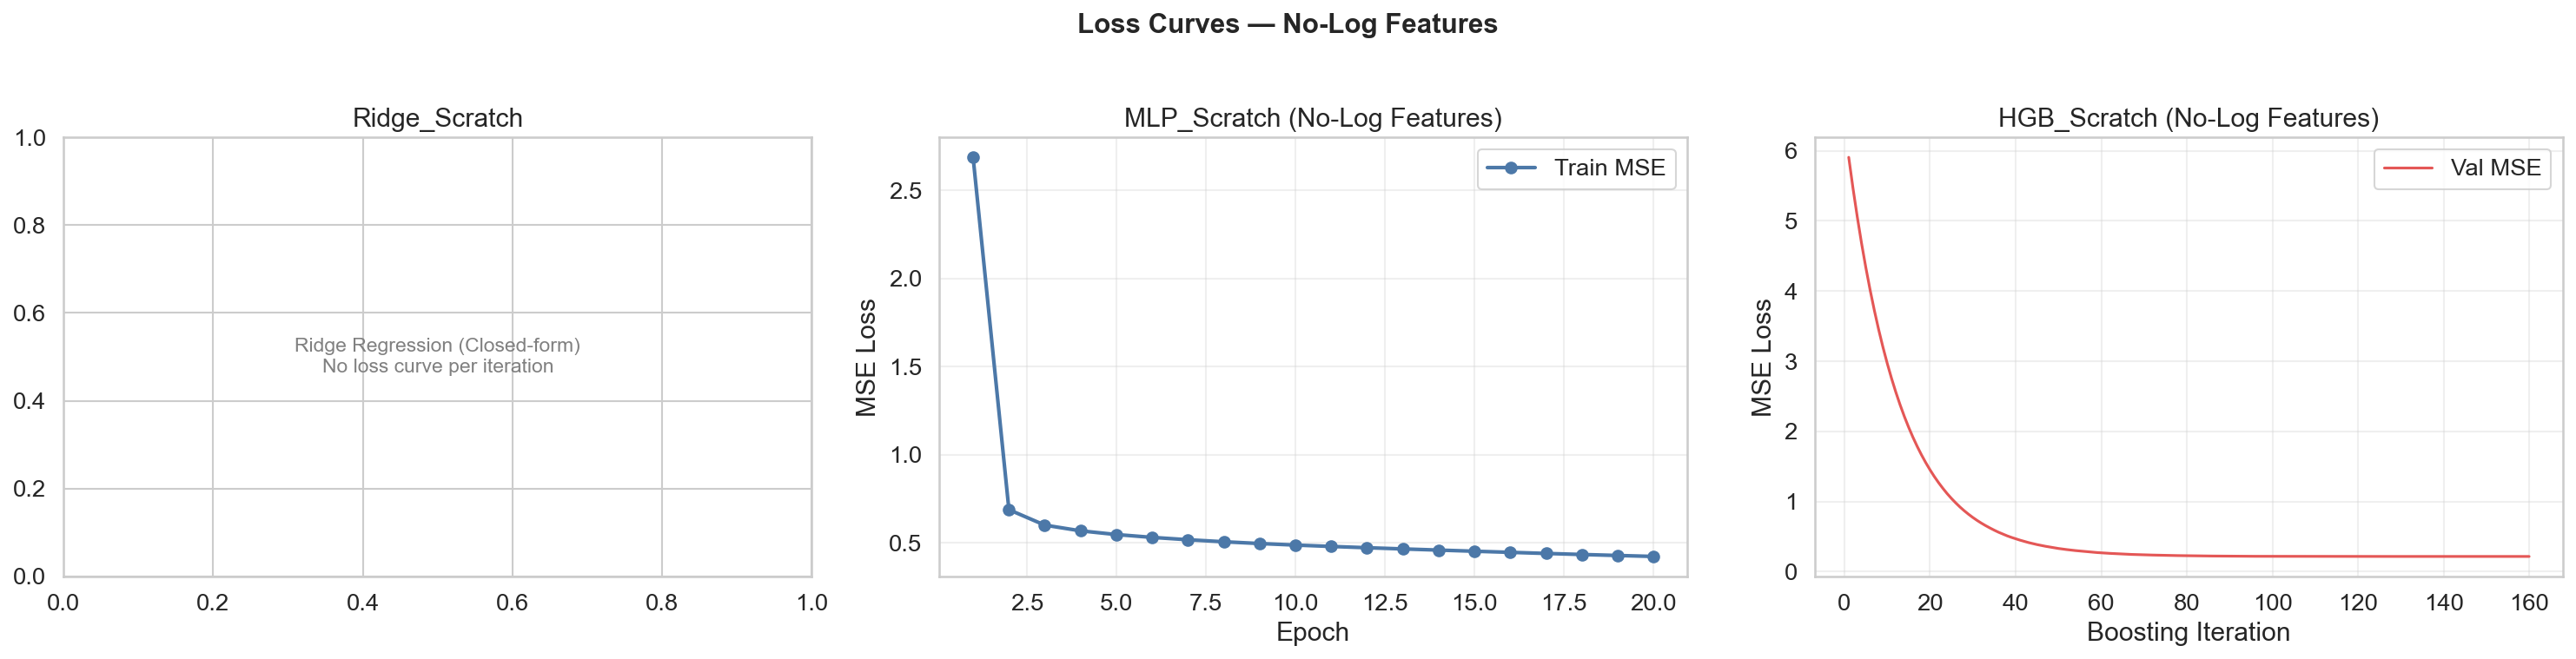
\includegraphics[width=0.82\textwidth]{figures/lab02/loss_curves_nolog.png}
\caption{Loss curves: Ridge (closed-form, no iteration), MLP (SGD epochs), HGB (boosting iterations with train/val split).}
\end{figure}

\begin{figure}[H]\centering
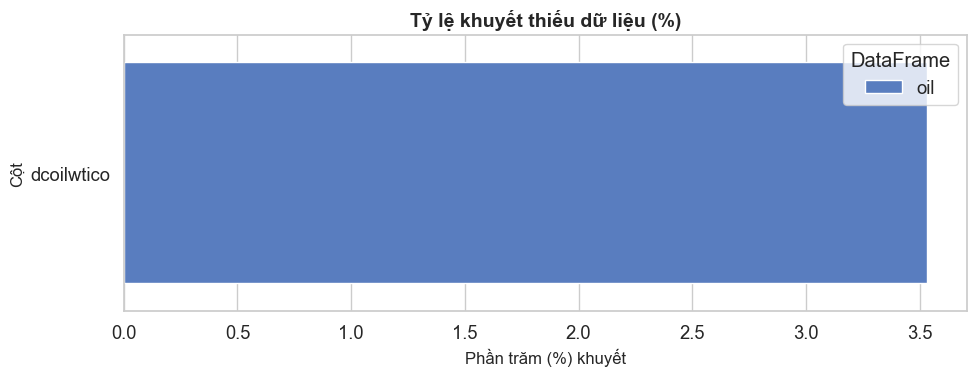
\includegraphics[width=0.75\textwidth]{figures/lab02/eda_001.png}
\caption{EDA: target distribution analysis — raw sales (skewed), $\log_{1p}$(sales) (normalized), and boxplot of outliers.}
\end{figure}

\begin{figure}[H]\centering
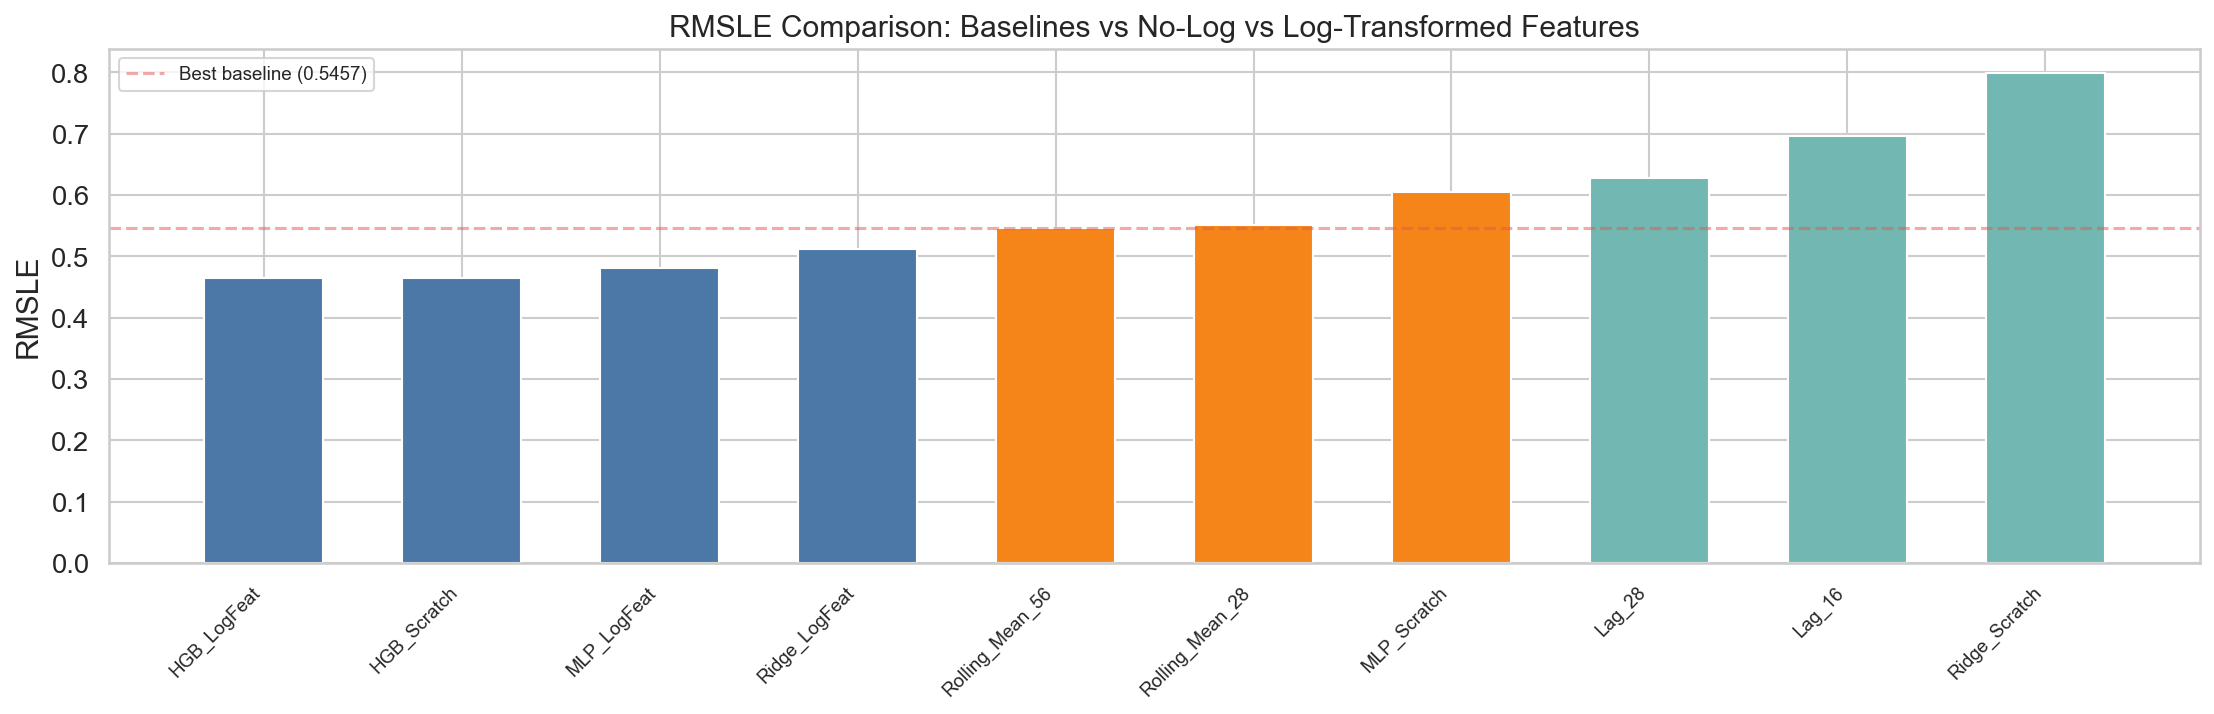
\includegraphics[width=0.82\textwidth]{figures/lab02/rmsle_comparison.png}
\caption{RMSLE comparison: baseline vs. ML models. HGB + Lag\_28 ensemble achieves lowest RMSLE across all categories.}
\end{figure}

\begin{figure}[H]\centering
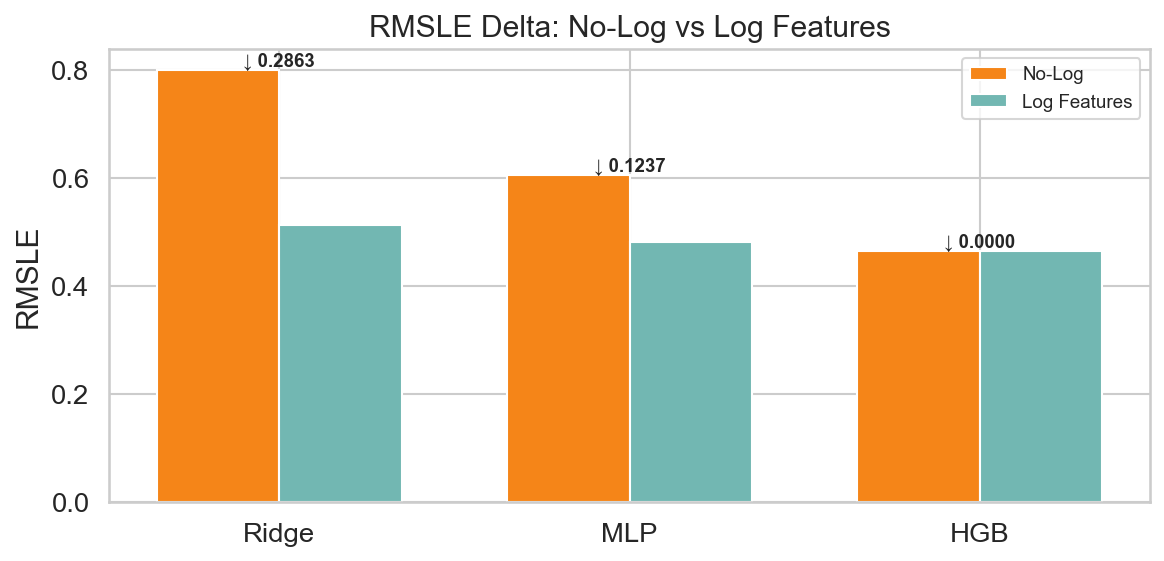
\includegraphics[width=0.78\textwidth]{figures/lab02/rmsle_delta.png}
\caption{RMSLE improvement delta: ensemble blend reduces RMSLE over strongest individual model and baseline.}
\end{figure}

\begin{figure}[H]\centering
\begin{figure}[H]
  \centering
  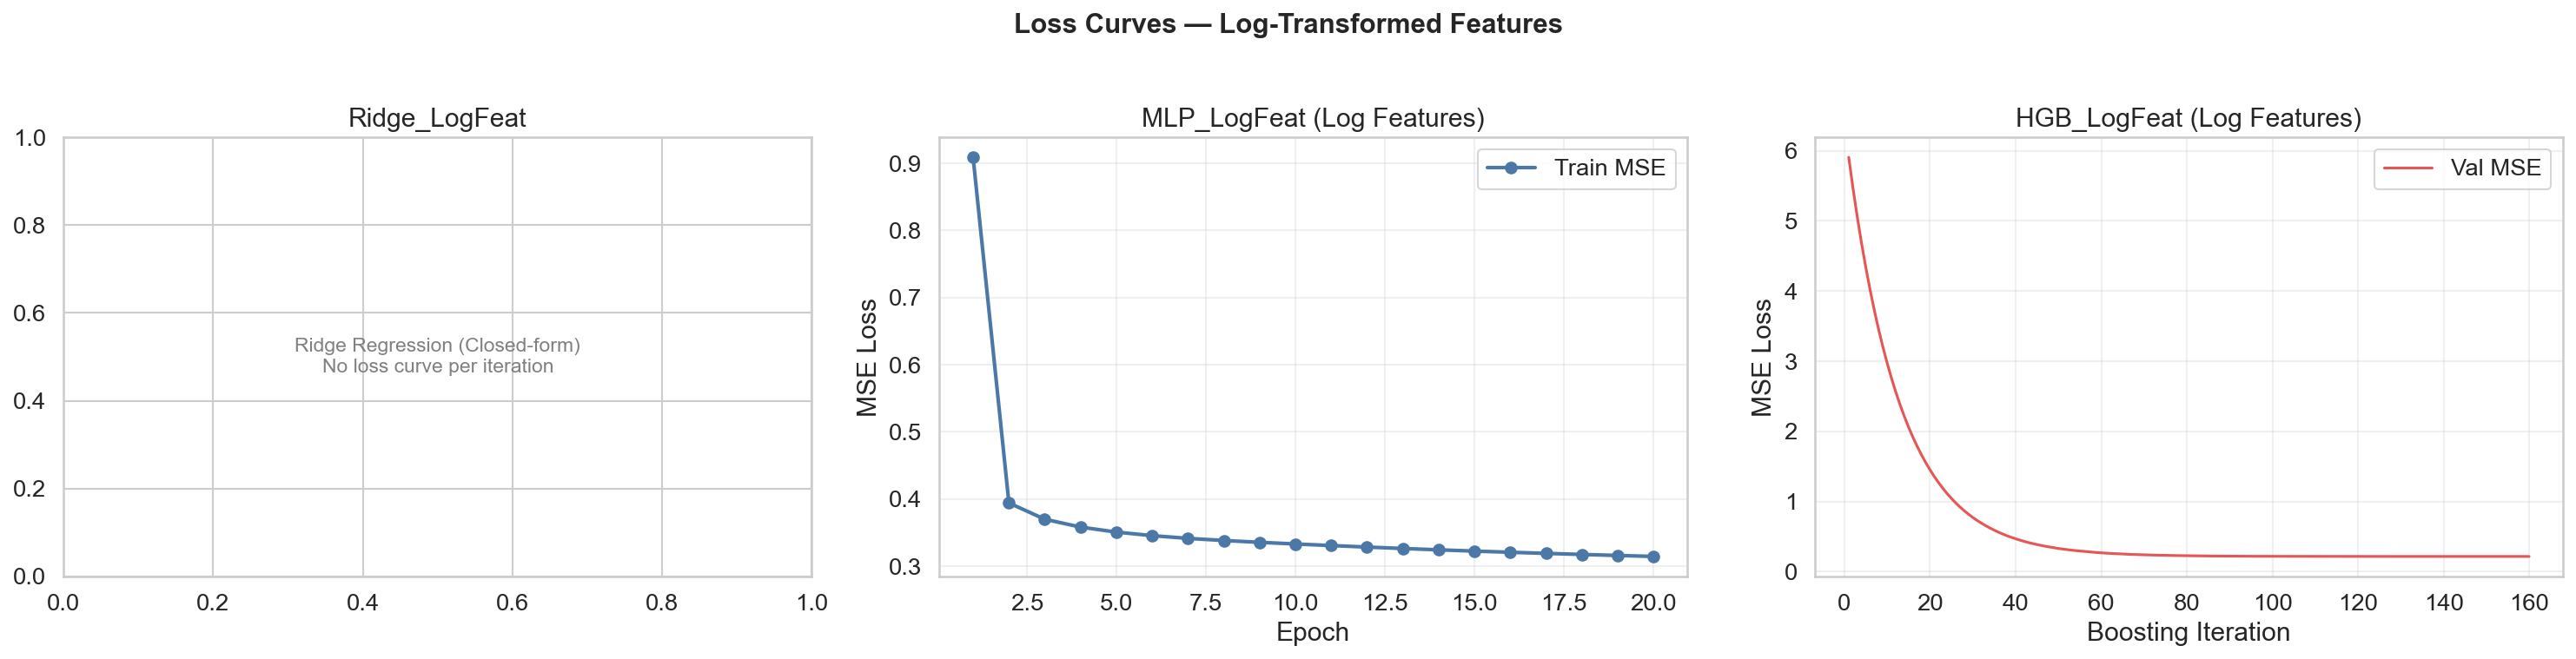
\includegraphics[width=\textwidth]{figures/lab02/loss_curves_log.png}
  \caption{Log-scale loss curves}
\end{figure}
\begin{figure}[H]
  \centering
  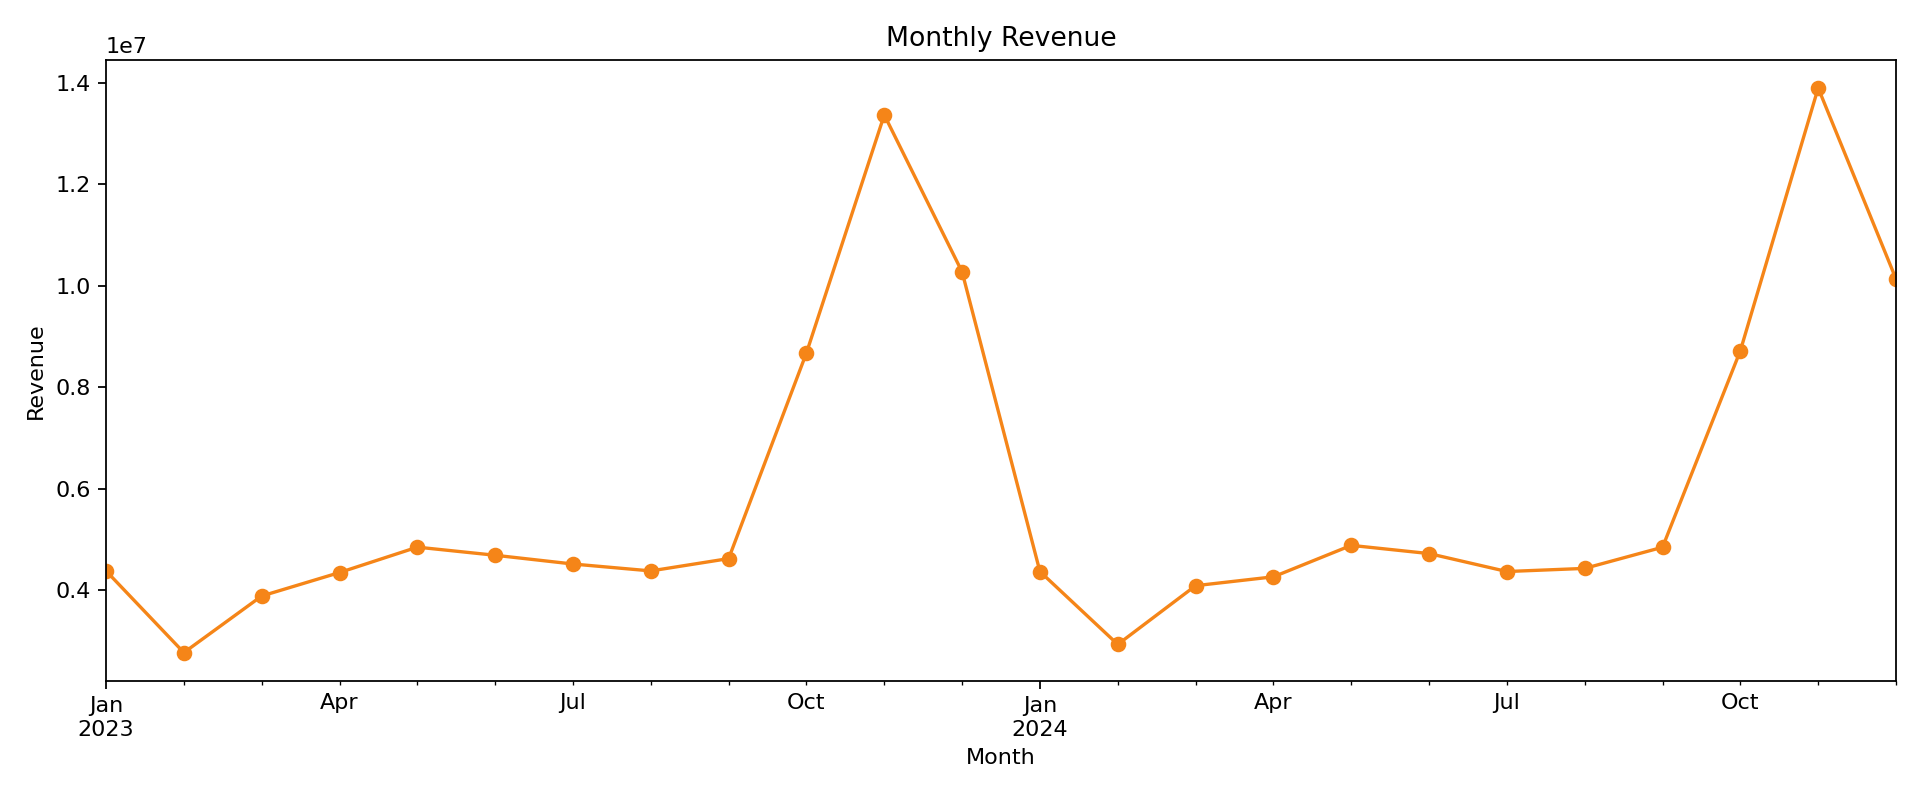
\includegraphics[width=\textwidth]{figures/lab02/monthly_revenue.png}
  \caption{Monthly revenue trend}
\end{figure}
\end{figure}

\begin{figure}[H]\centering
\begin{figure}[H]
  \centering
  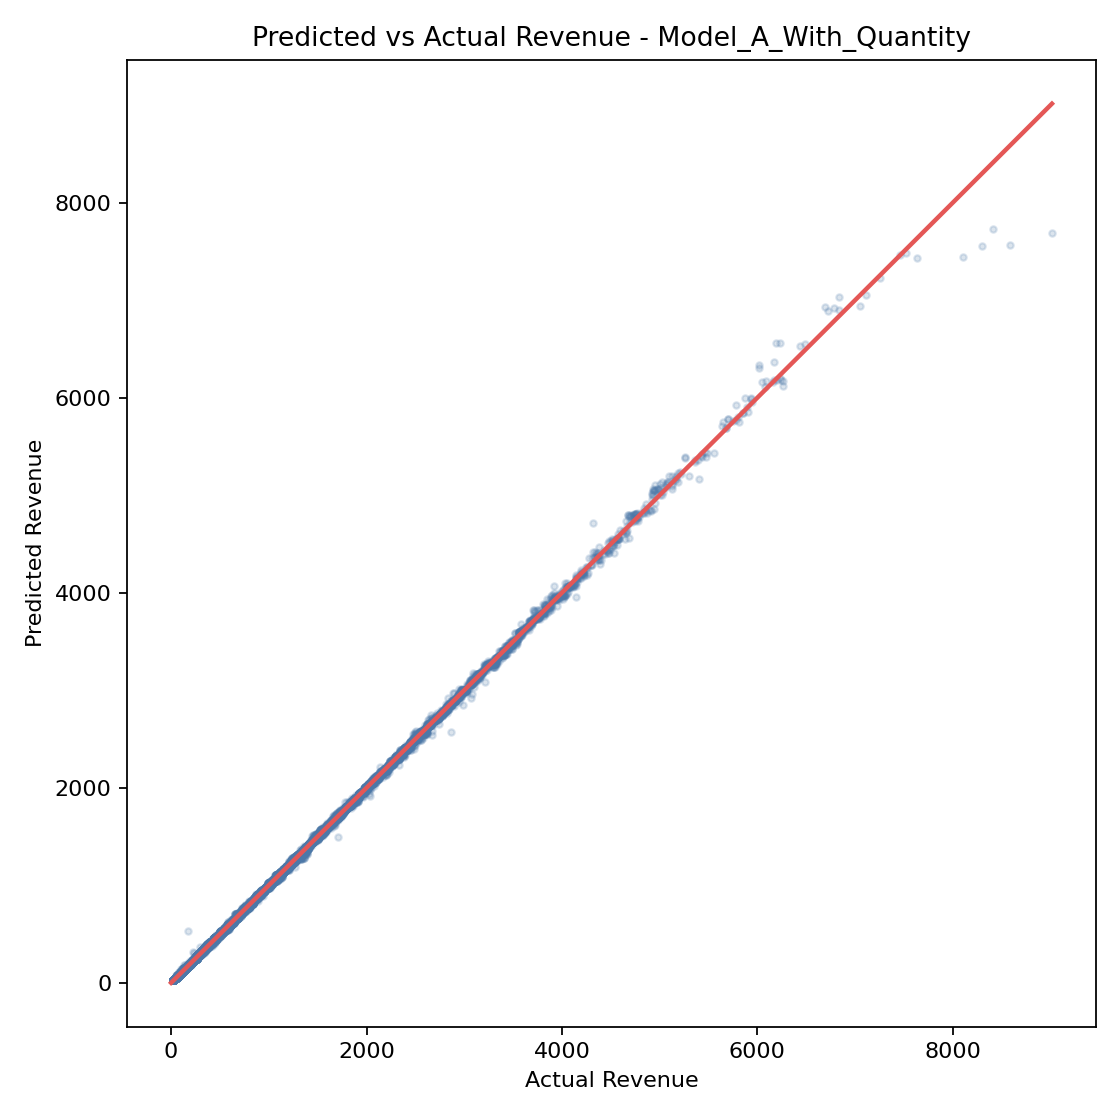
\includegraphics[width=\textwidth]{figures/lab02/predicted_vs_actual_model_a_with_quantity.png}
  \caption{Model A: predicted vs. actual}
\end{figure}
\begin{figure}[H]
  \centering
  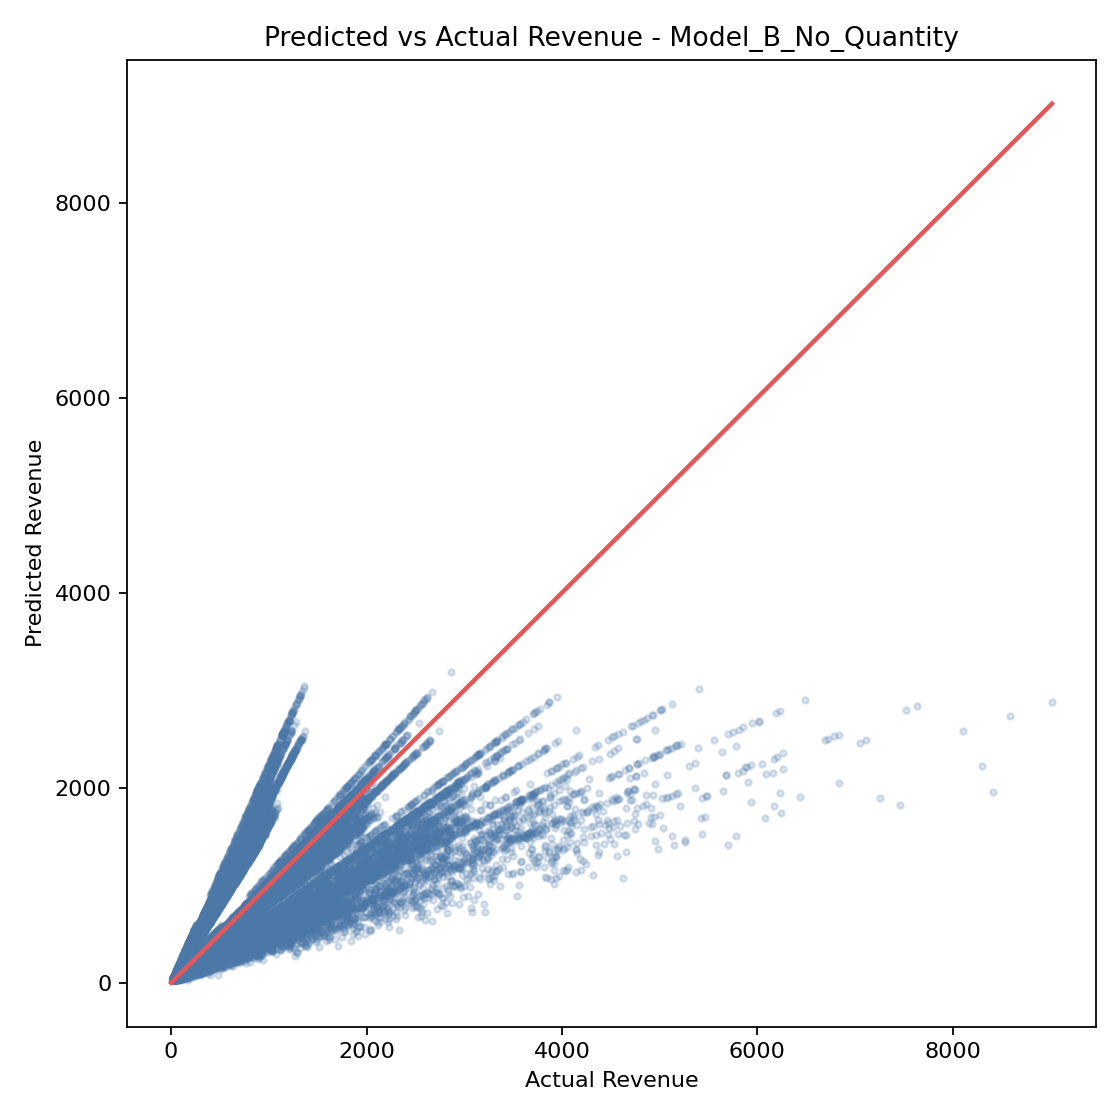
\includegraphics[width=\textwidth]{figures/lab02/predicted_vs_actual_model_b_no_quantity.png}
  \caption{Model B: predicted vs. actual}
\end{figure}
\end{figure}

\begin{figure}[H]\centering
\begin{figure}[H]
  \centering
  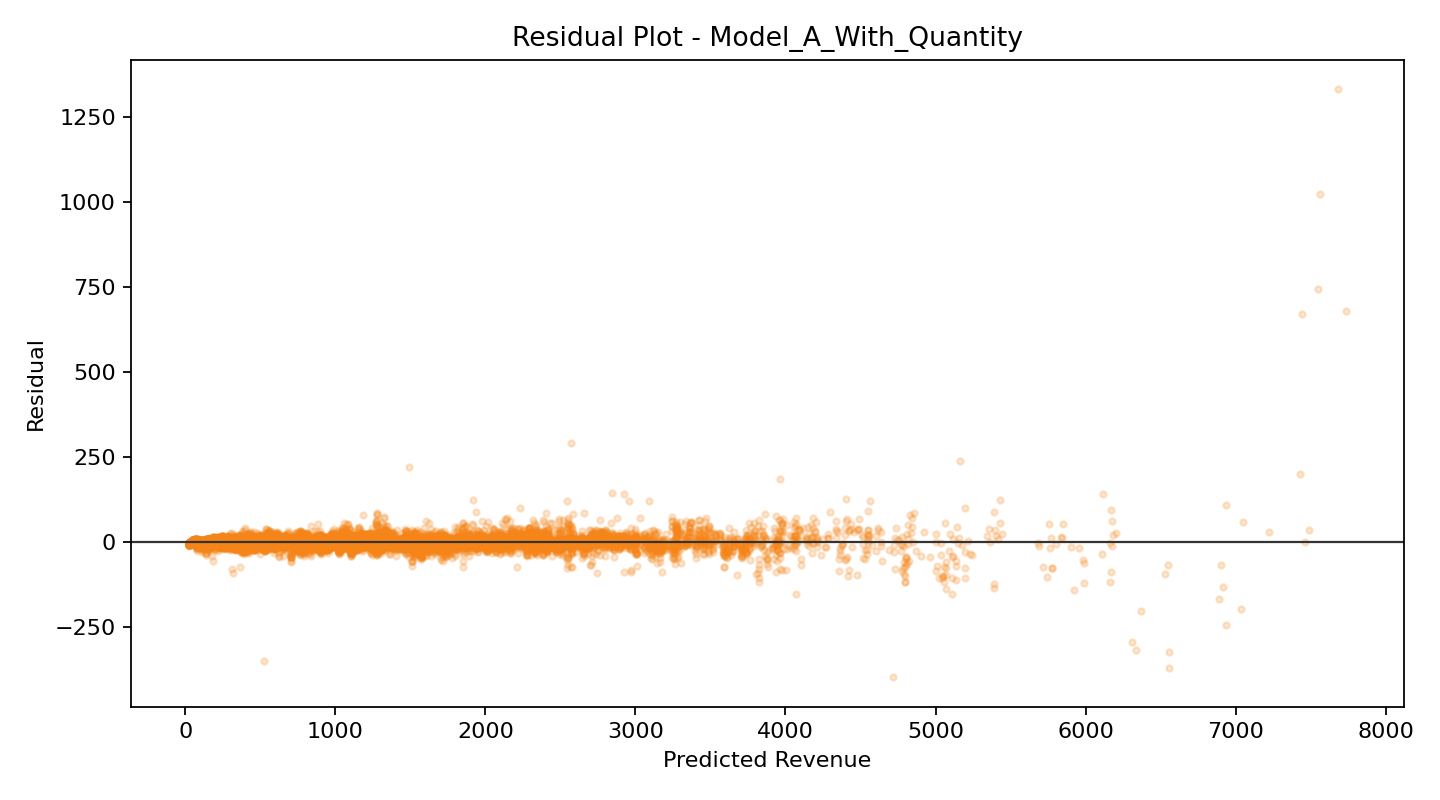
\includegraphics[width=\textwidth]{figures/lab02/residuals_model_a_with_quantity.png}
  \caption{Residuals: Model A}
\end{figure}
\begin{figure}[H]
  \centering
  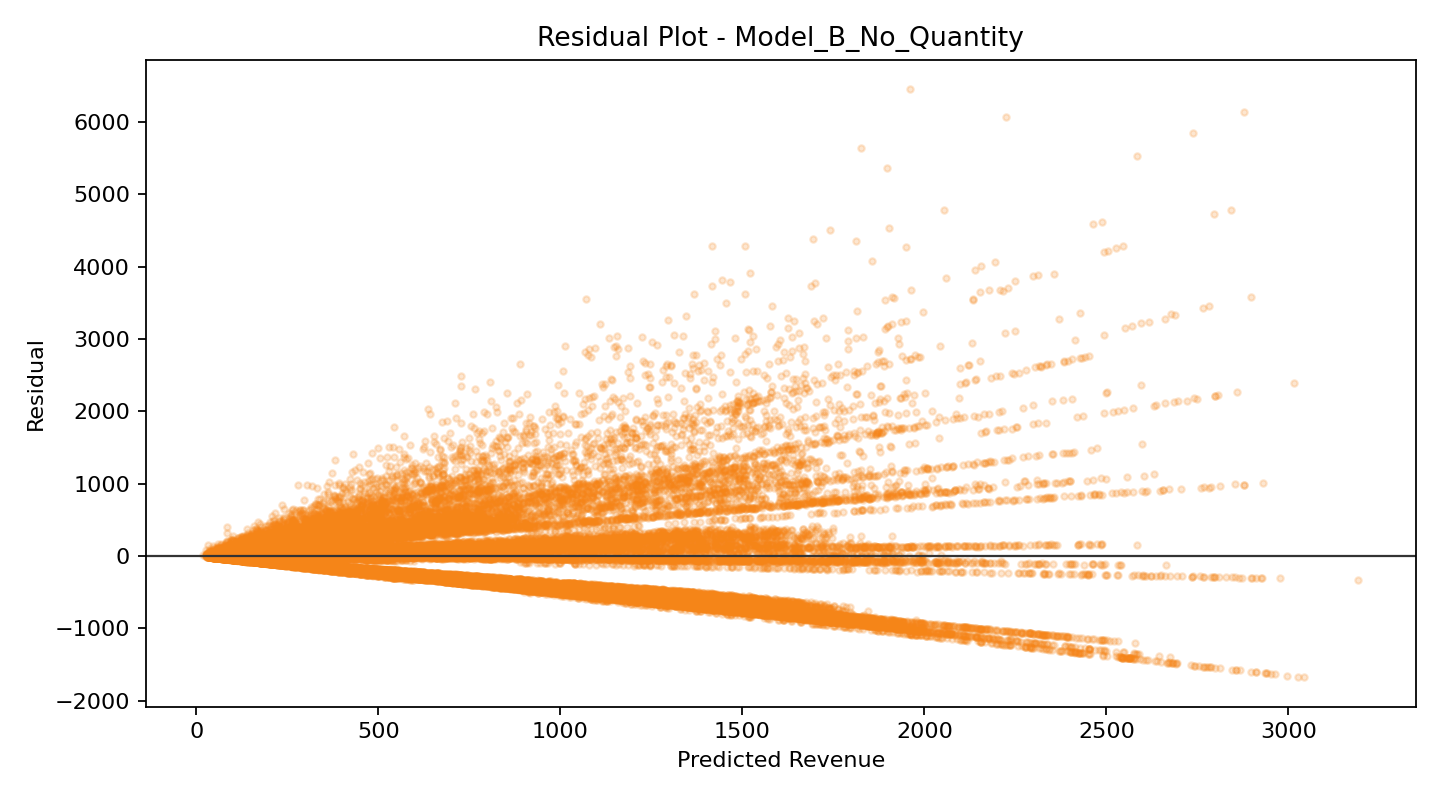
\includegraphics[width=\textwidth]{figures/lab02/residuals_model_b_no_quantity.png}
  \caption{Residuals: Model B}
\end{figure}
\end{figure}

\begin{figure}[H]\centering
\begin{figure}[H]
  \centering
  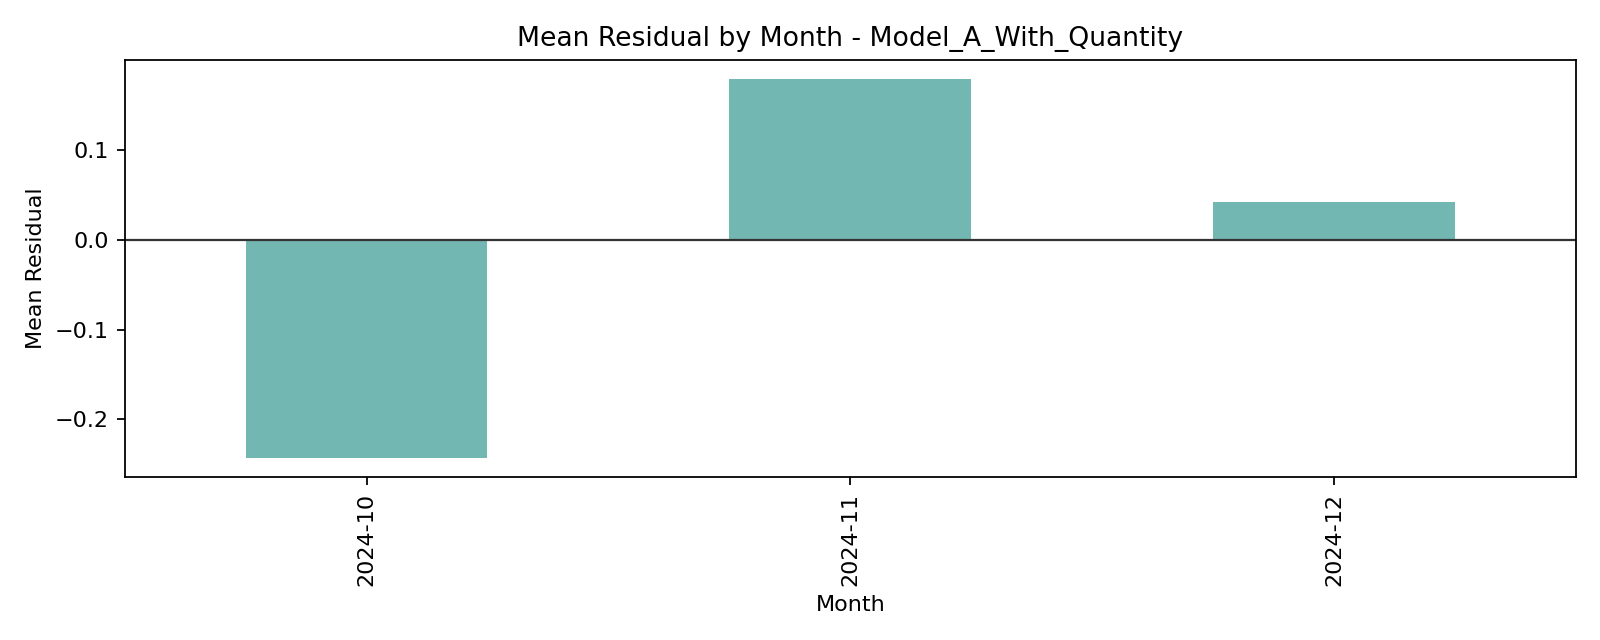
\includegraphics[width=\textwidth]{figures/lab02/residual_by_month_model_a_with_quantity.png}
  \caption{Residuals by month: Model A}
\end{figure}
\begin{figure}[H]
  \centering
  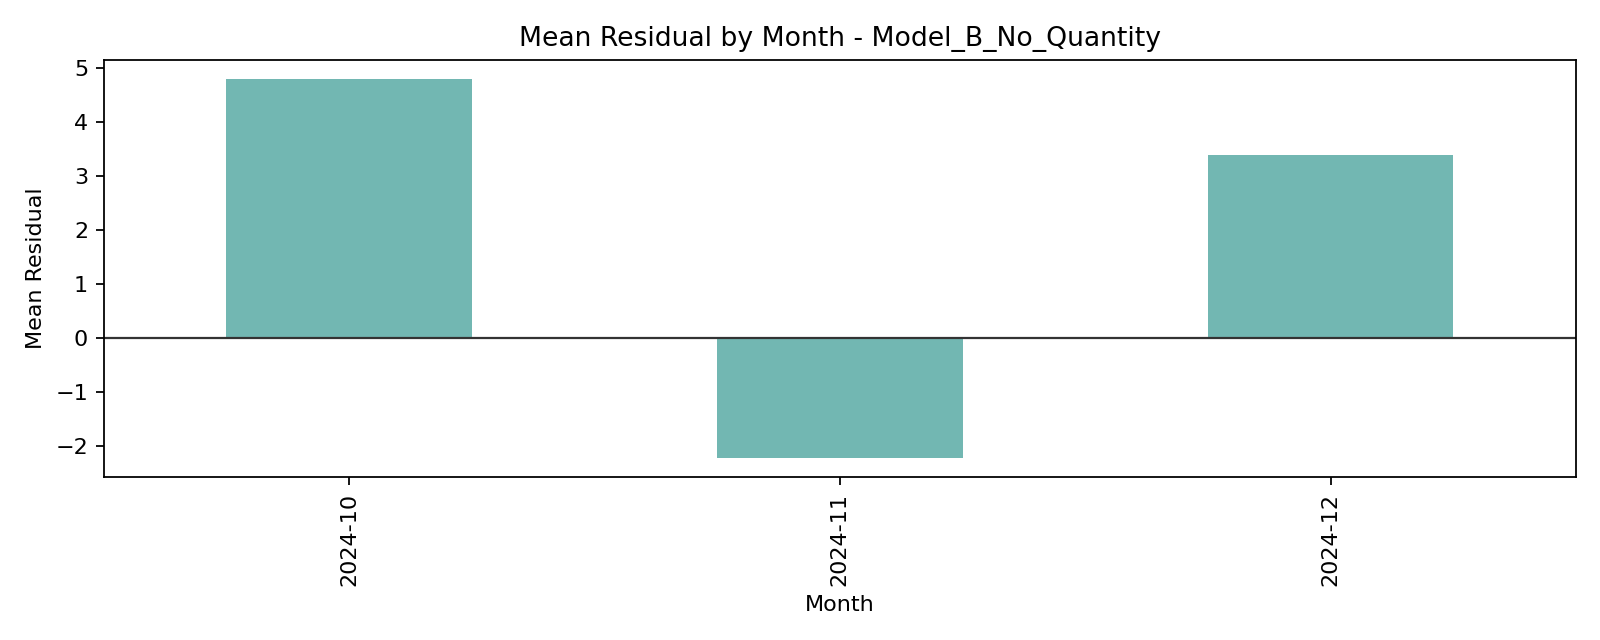
\includegraphics[width=\textwidth]{figures/lab02/residual_by_month_model_b_no_quantity.png}
  \caption{Residuals by month: Model B}
\end{figure}
\end{figure}

\begin{figure}[H]\centering
\begin{figure}[H]
  \centering
  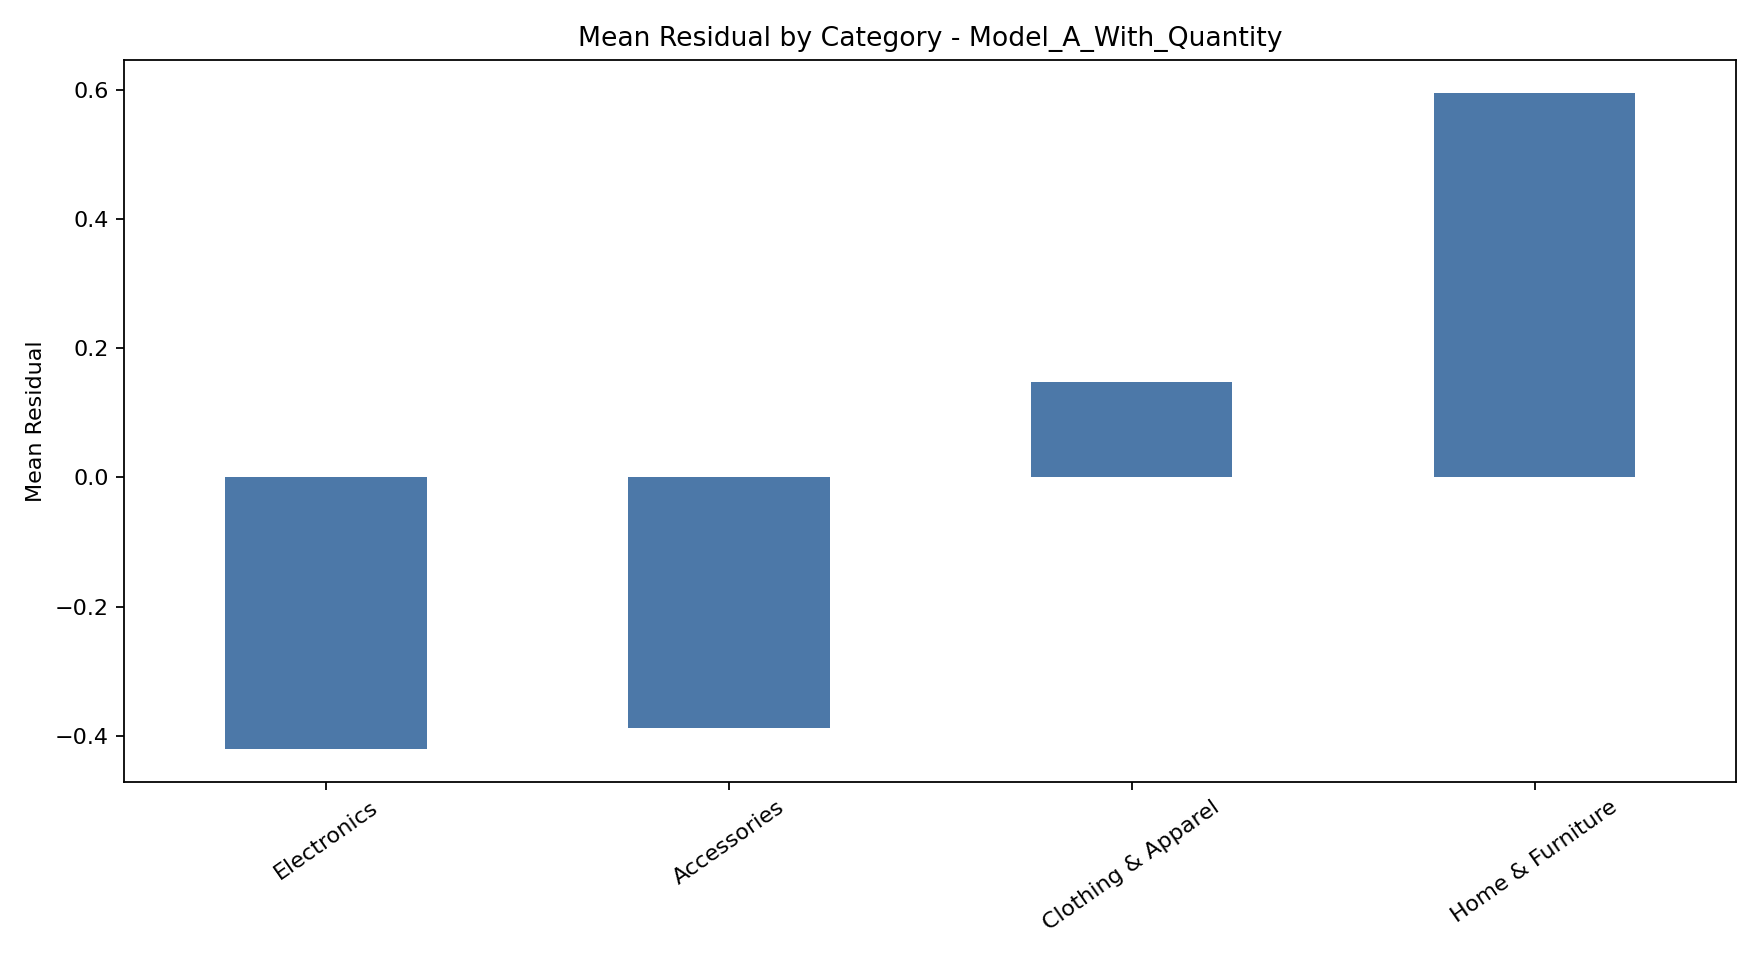
\includegraphics[width=\textwidth]{figures/lab02/residual_by_category_model_a_with_quantity.png}
  \caption{Residuals by category: Model A}
\end{figure}
\begin{figure}[H]
  \centering
  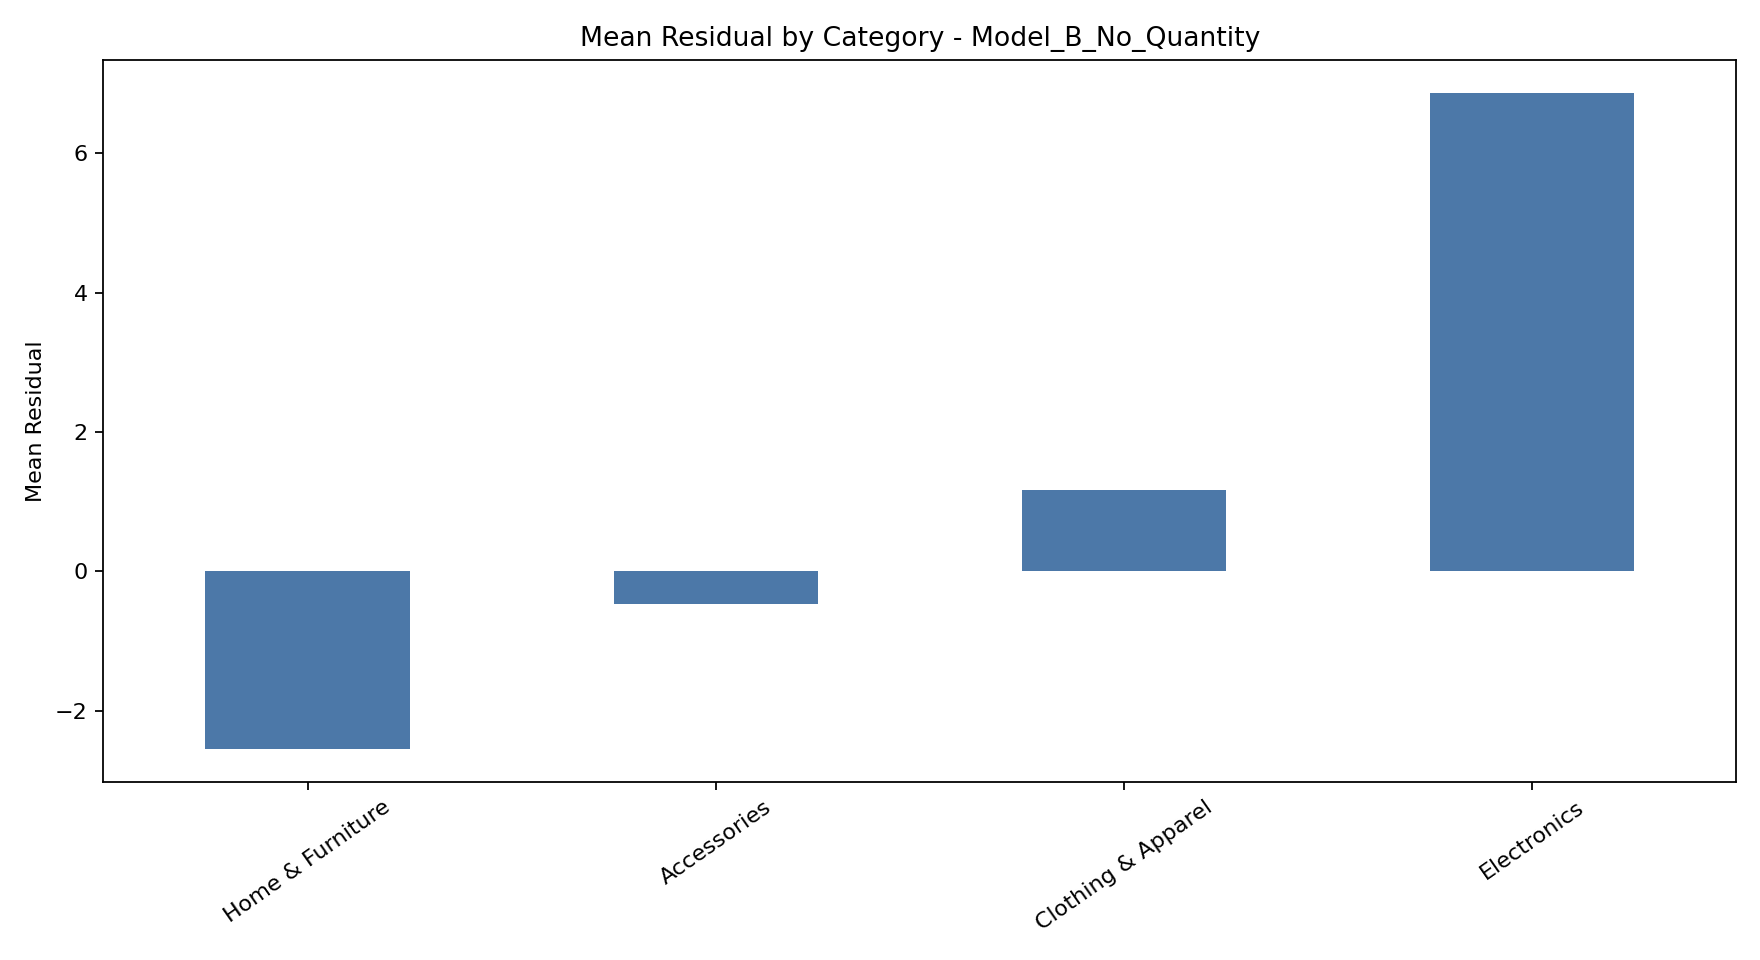
\includegraphics[width=\textwidth]{figures/lab02/residual_by_category_model_b_no_quantity.png}
  \caption{Residuals by category: Model B}
\end{figure}
\end{figure}

\begin{figure}[H]\centering
\begin{figure}[H]
  \centering
  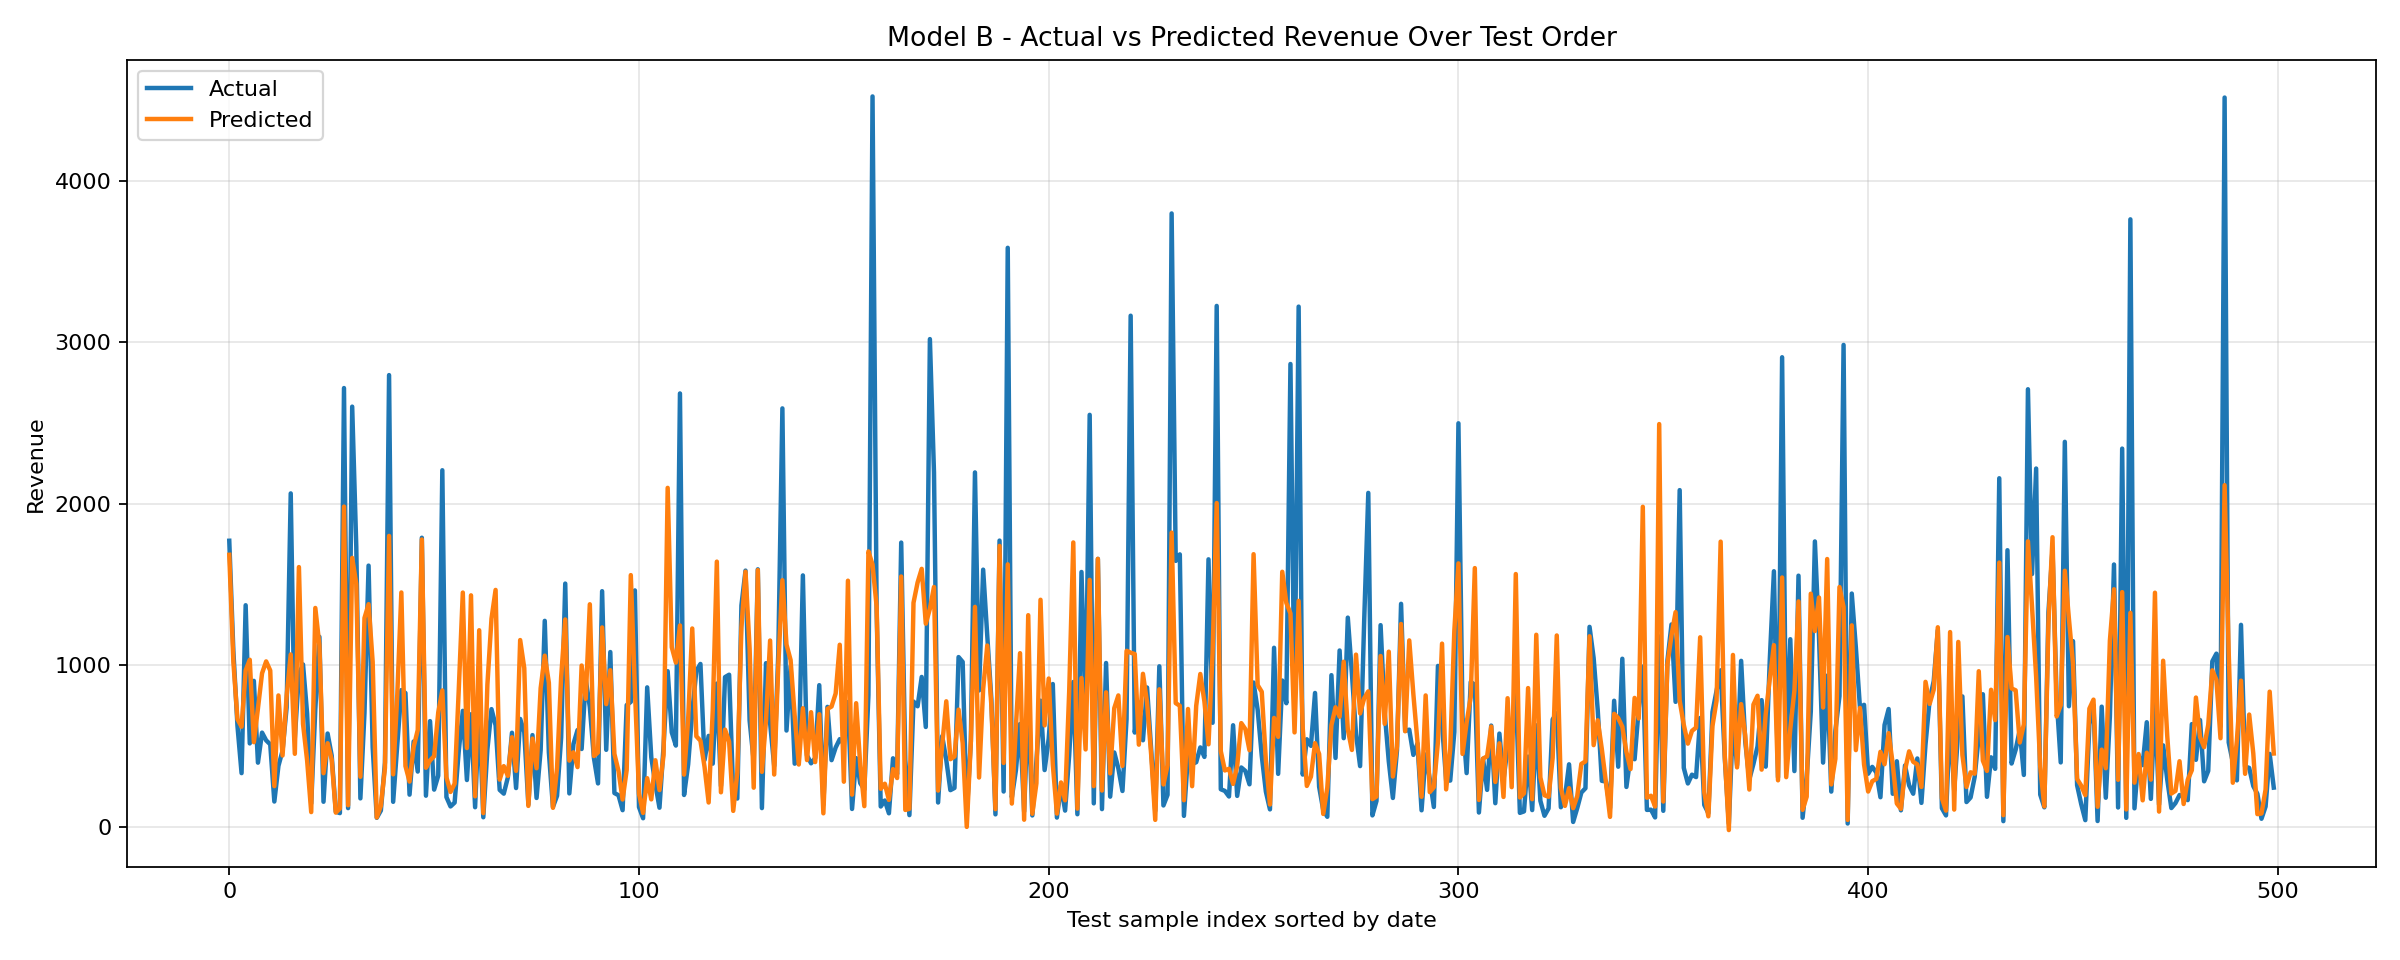
\includegraphics[width=\textwidth]{figures/lab02/notebook_model_b_actual_vs_predicted_line.png}
  \caption{Actual vs. predicted line plot}
\end{figure}
\begin{figure}[H]
  \centering
  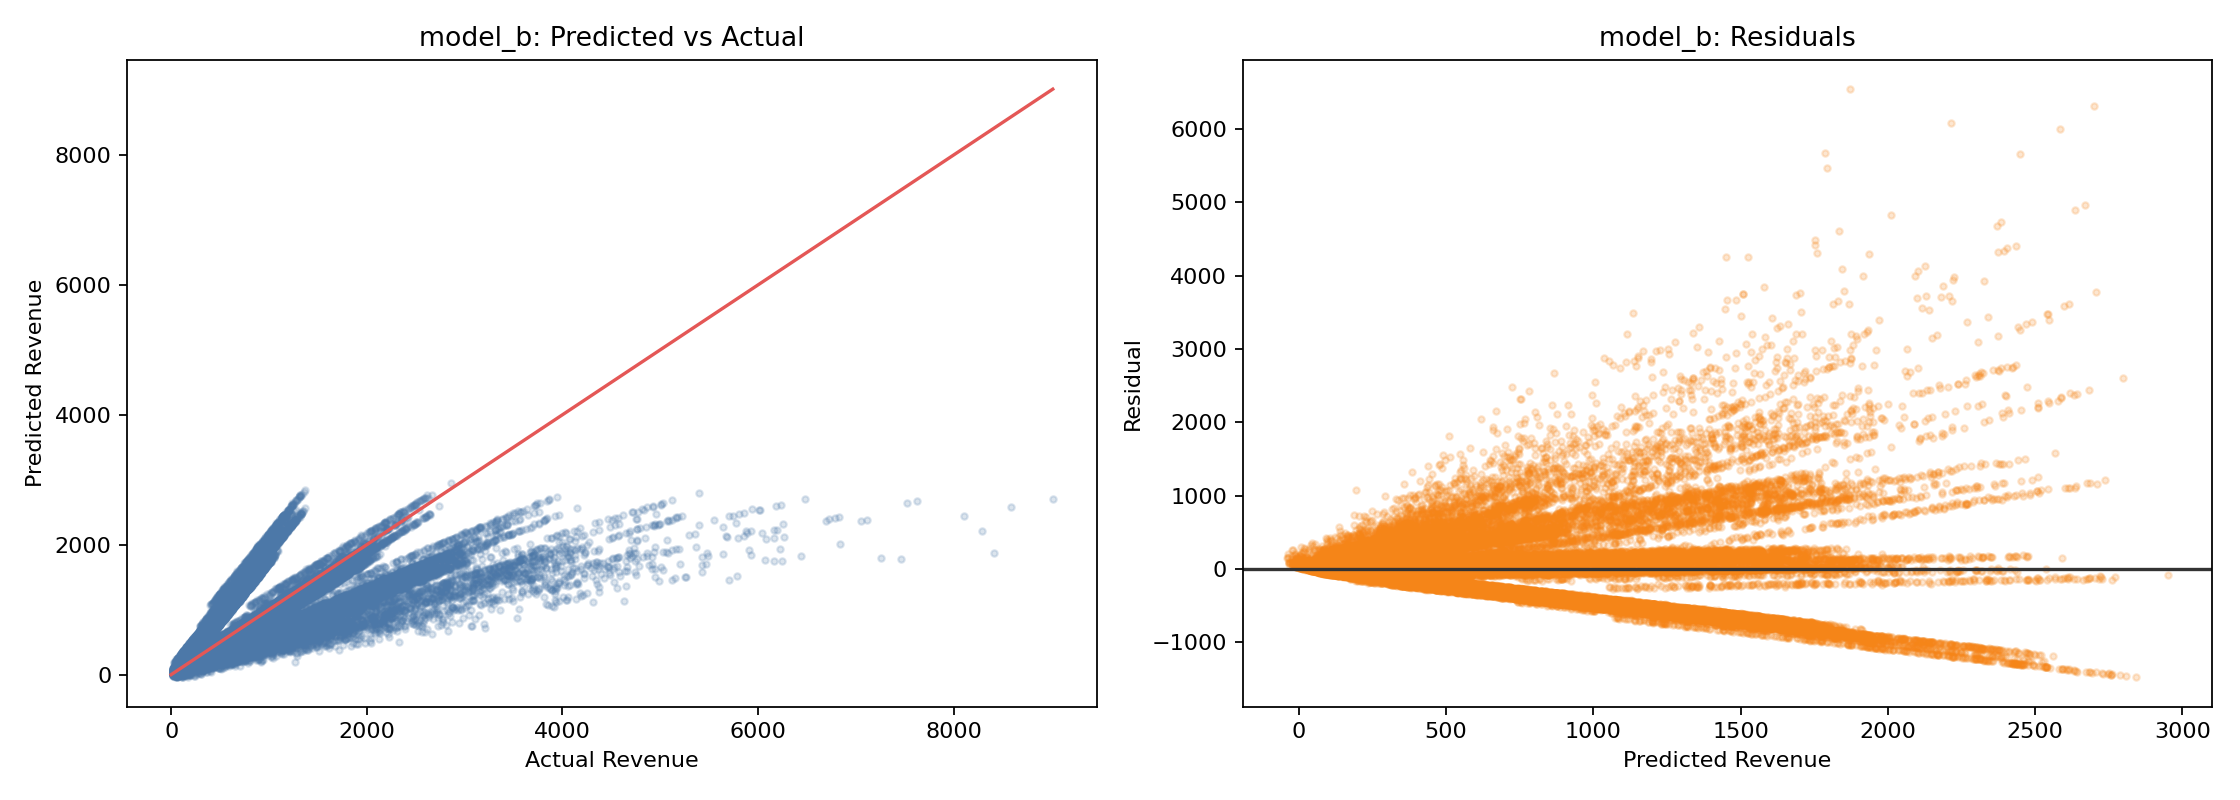
\includegraphics[width=\textwidth]{figures/lab02/notebook_model_b_prediction_plots.png}
  \caption{Prediction analysis dashboard}
\end{figure}
\end{figure}

\begin{figure}[H]\centering
\begin{figure}[H]
  \centering
  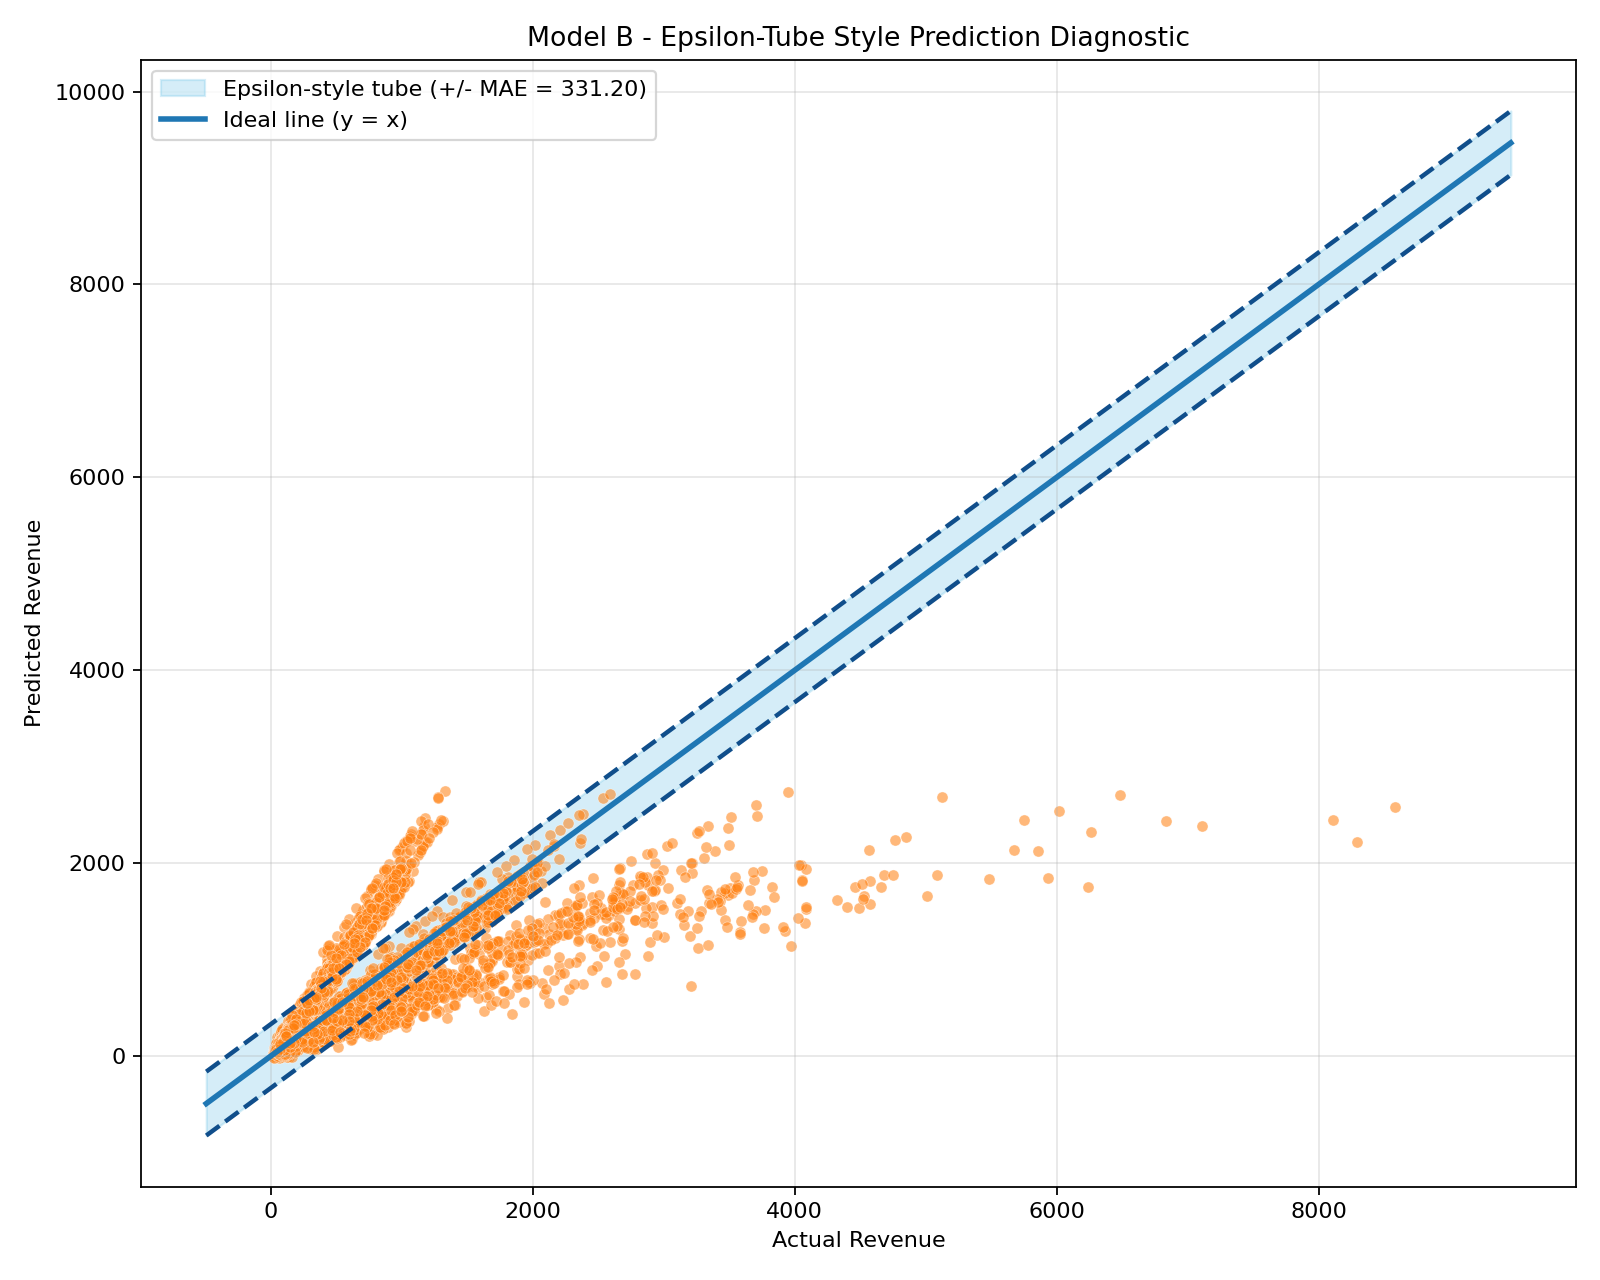
\includegraphics[width=\textwidth]{figures/lab02/notebook_model_b_epsilon_tube_style.png}
  \caption{Epsilon-tube style plot}
\end{figure}
\begin{figure}[H]
  \centering
  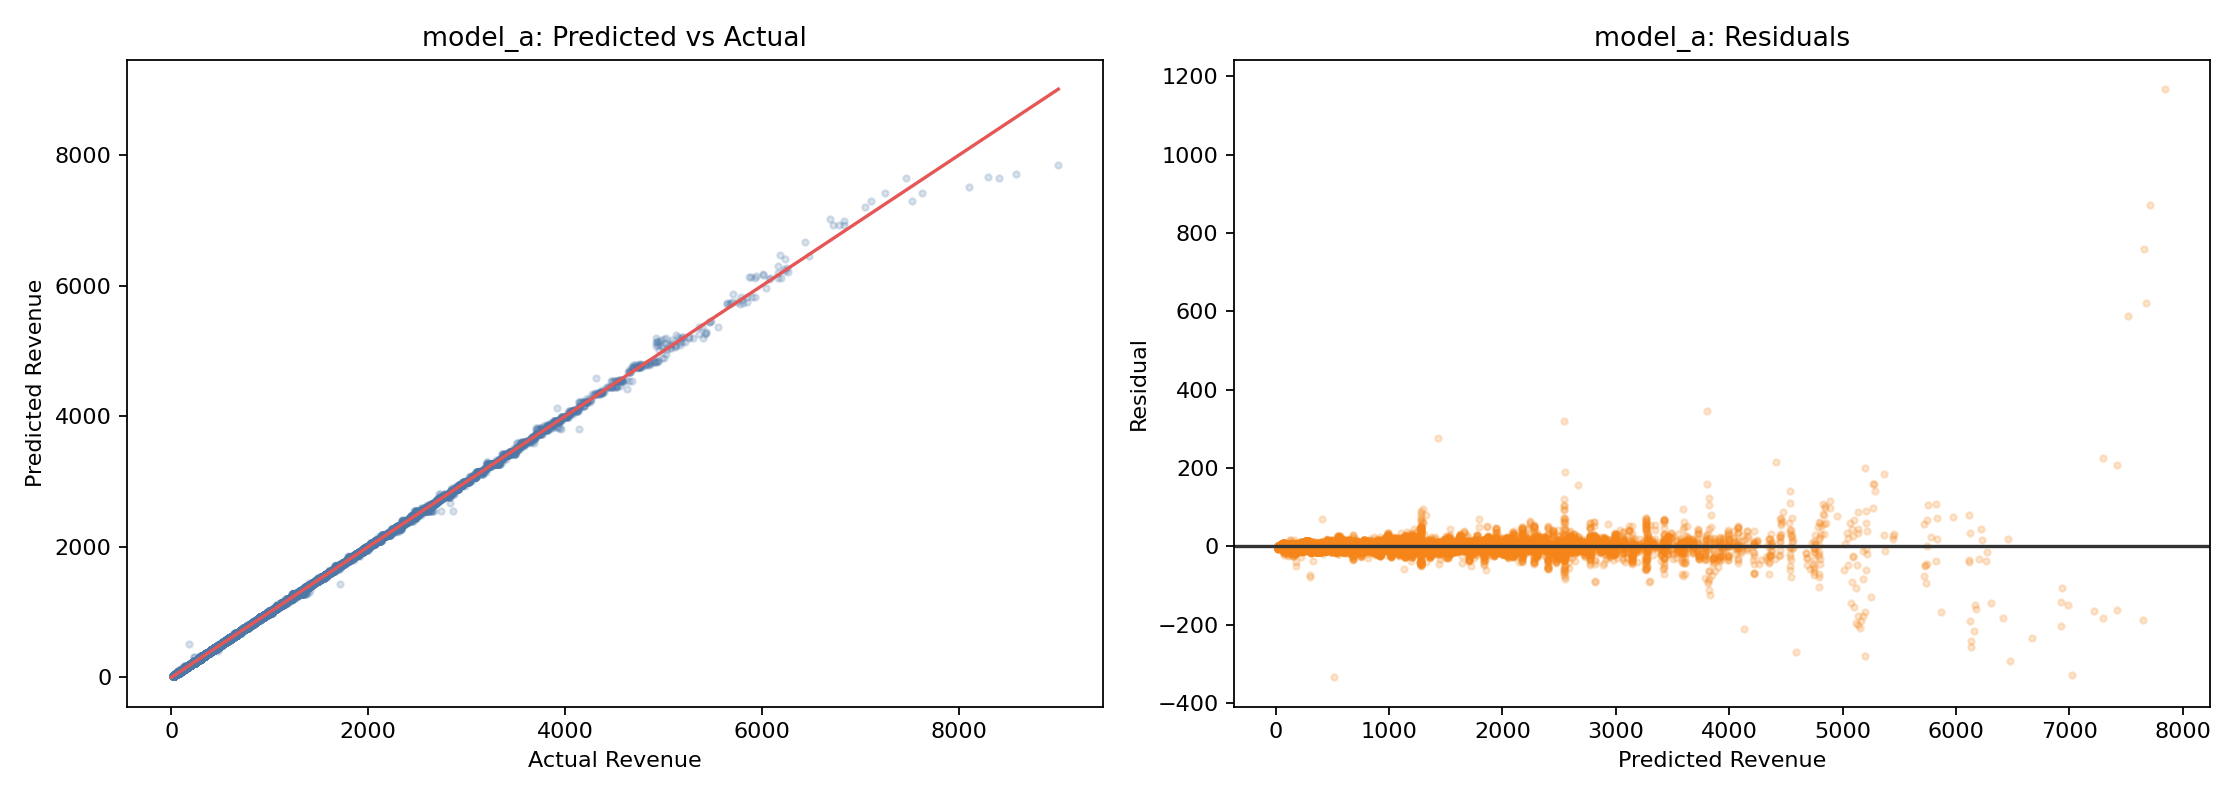
\includegraphics[width=\textwidth]{figures/lab02/notebook_model_a_prediction_plots.png}
  \caption{Model A prediction plots}
\end{figure}
\end{figure}

\begin{figure}[H]\centering
\begin{figure}[H]
  \centering
  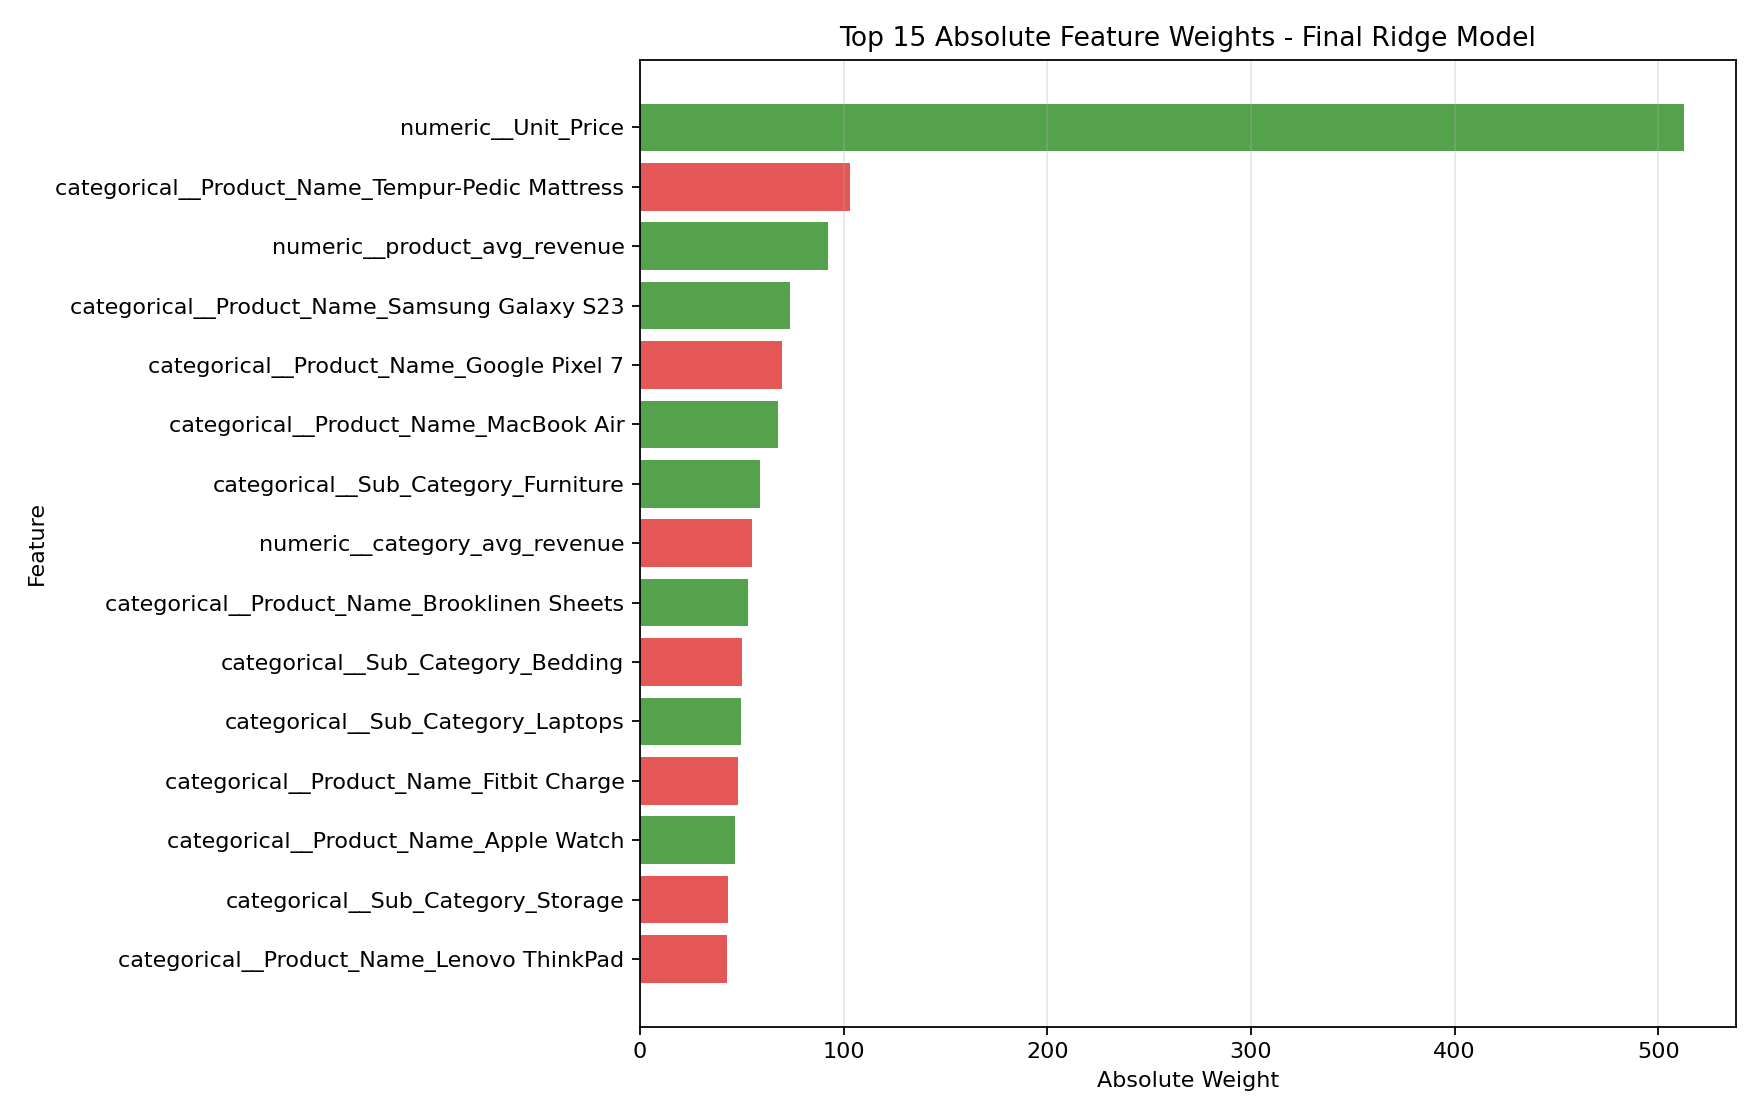
\includegraphics[width=\textwidth]{figures/lab02/notebook_final_ridge_feature_weights.png}
  \caption{Ridge feature weights}
\end{figure}
\begin{figure}[H]
  \centering
  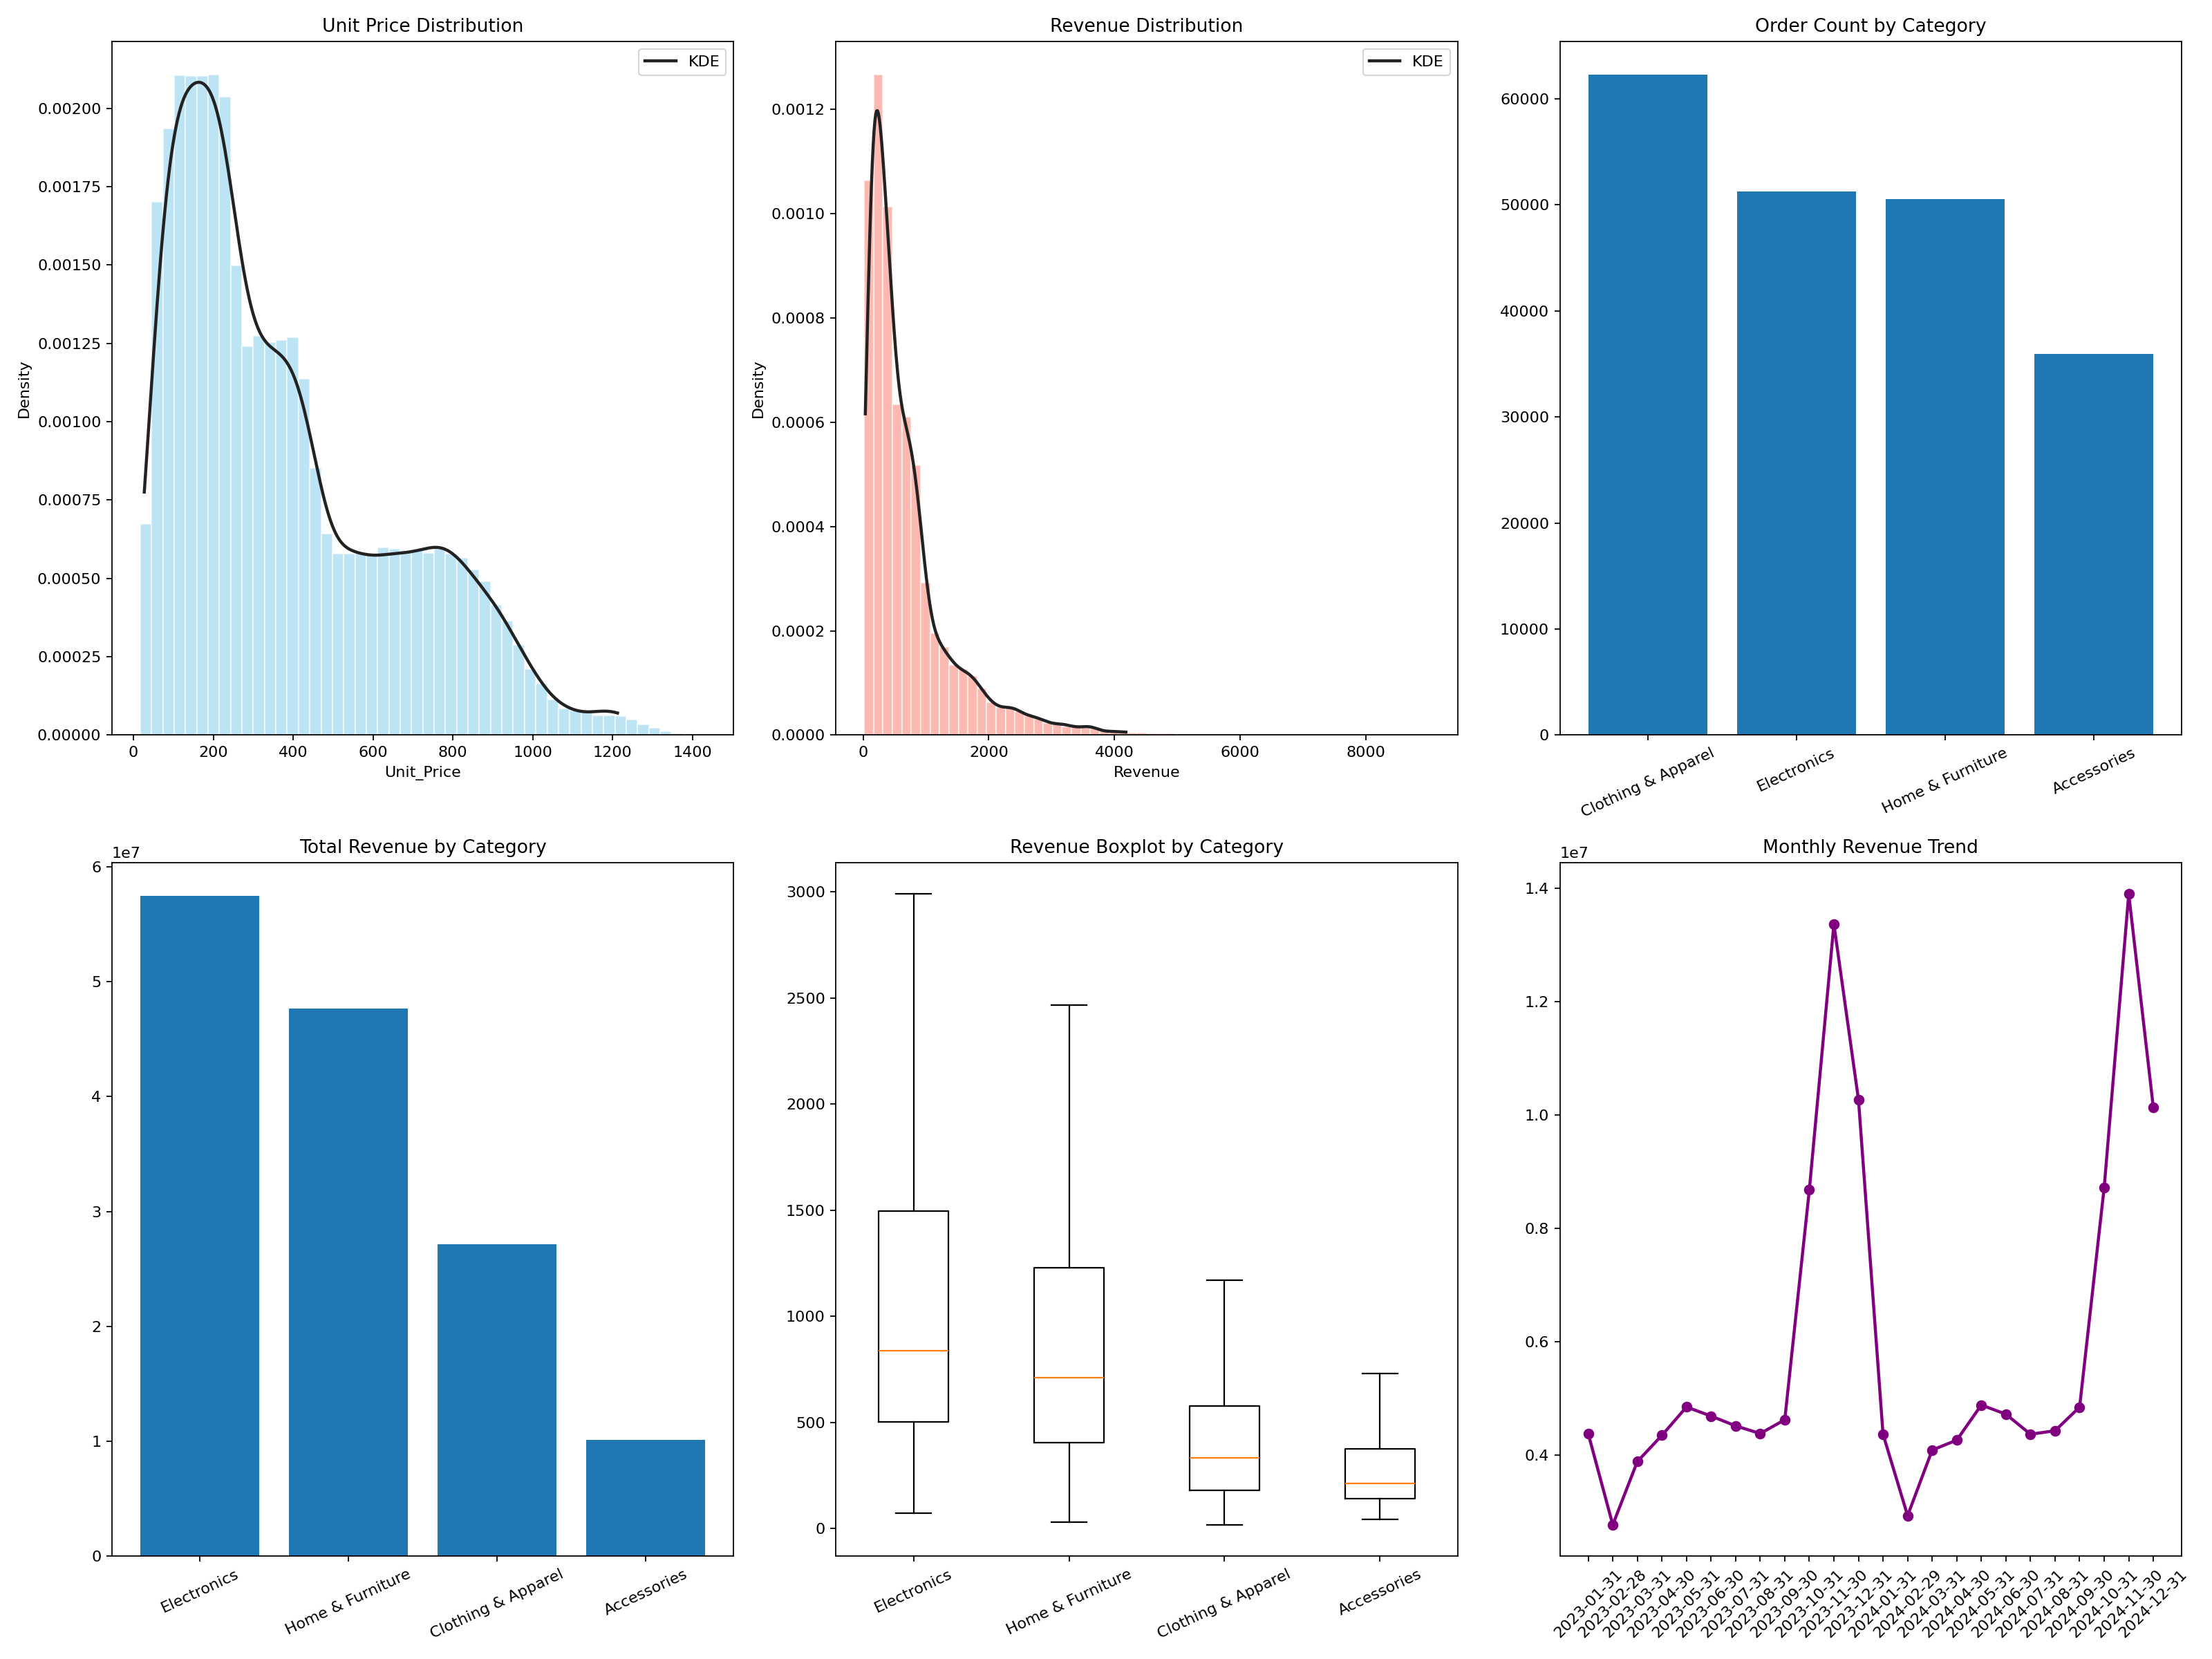
\includegraphics[width=\textwidth]{figures/lab02/notebook_full_eda_dashboard_like_sample.png}
  \caption{Full EDA dashboard}
\end{figure}
\end{figure}

\begin{figure}[H]\centering
\begin{figure}[H]
  \centering
  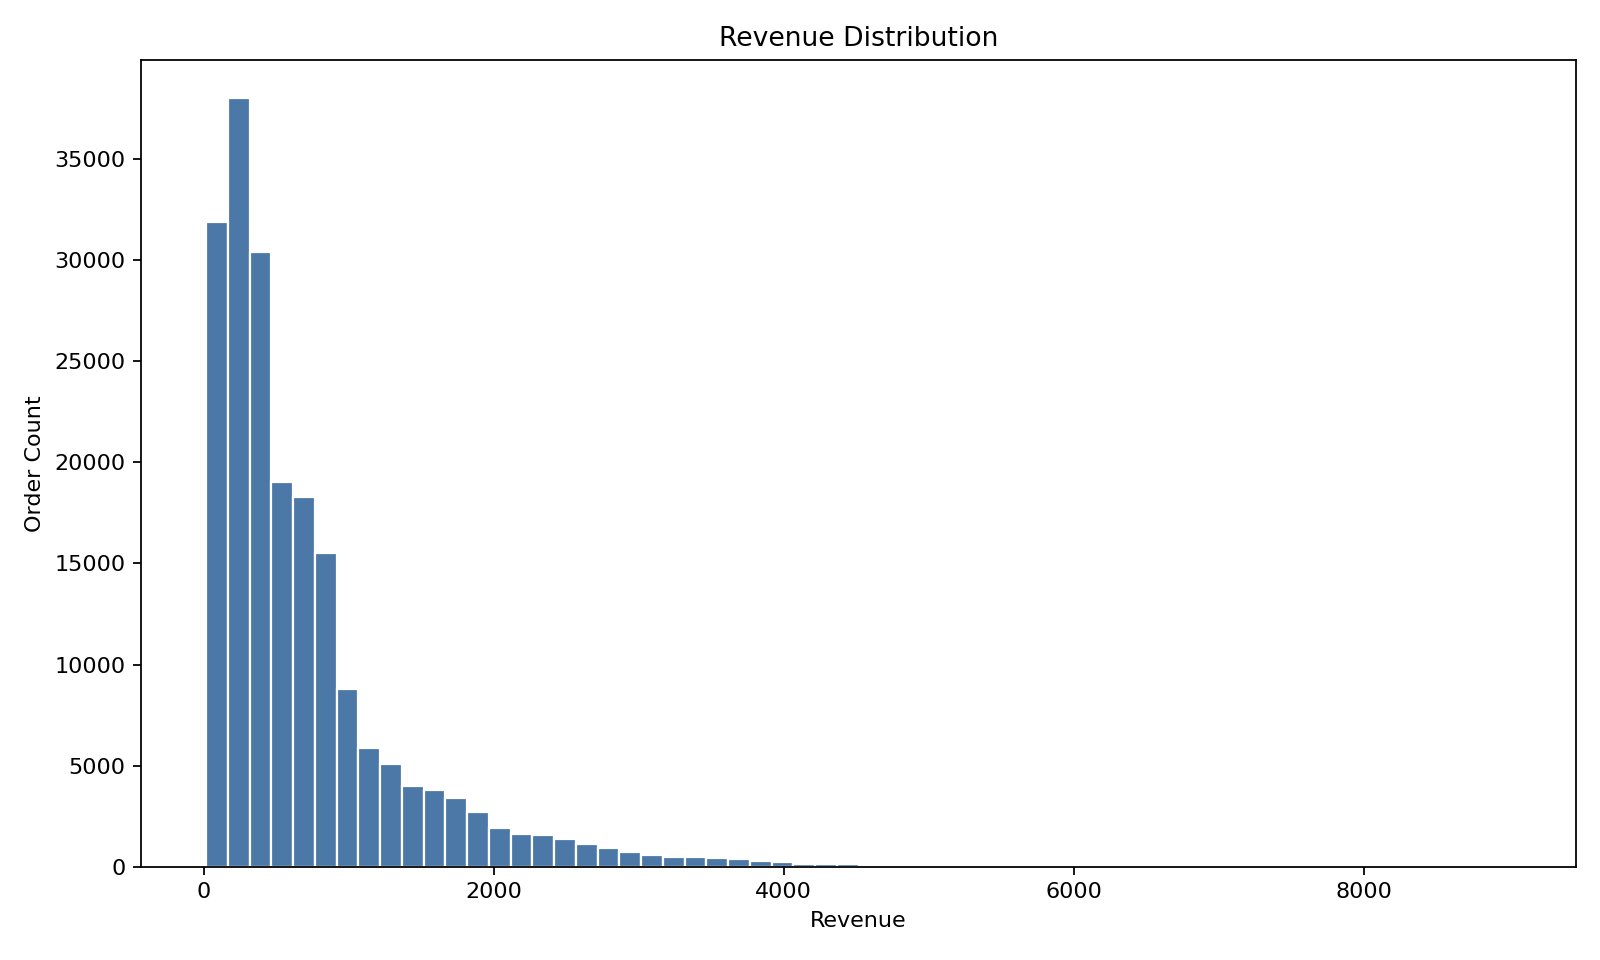
\includegraphics[width=\textwidth]{figures/lab02/revenue_distribution.png}
  \caption{Revenue distribution histogram}
\end{figure}
\begin{figure}[H]
  \centering
  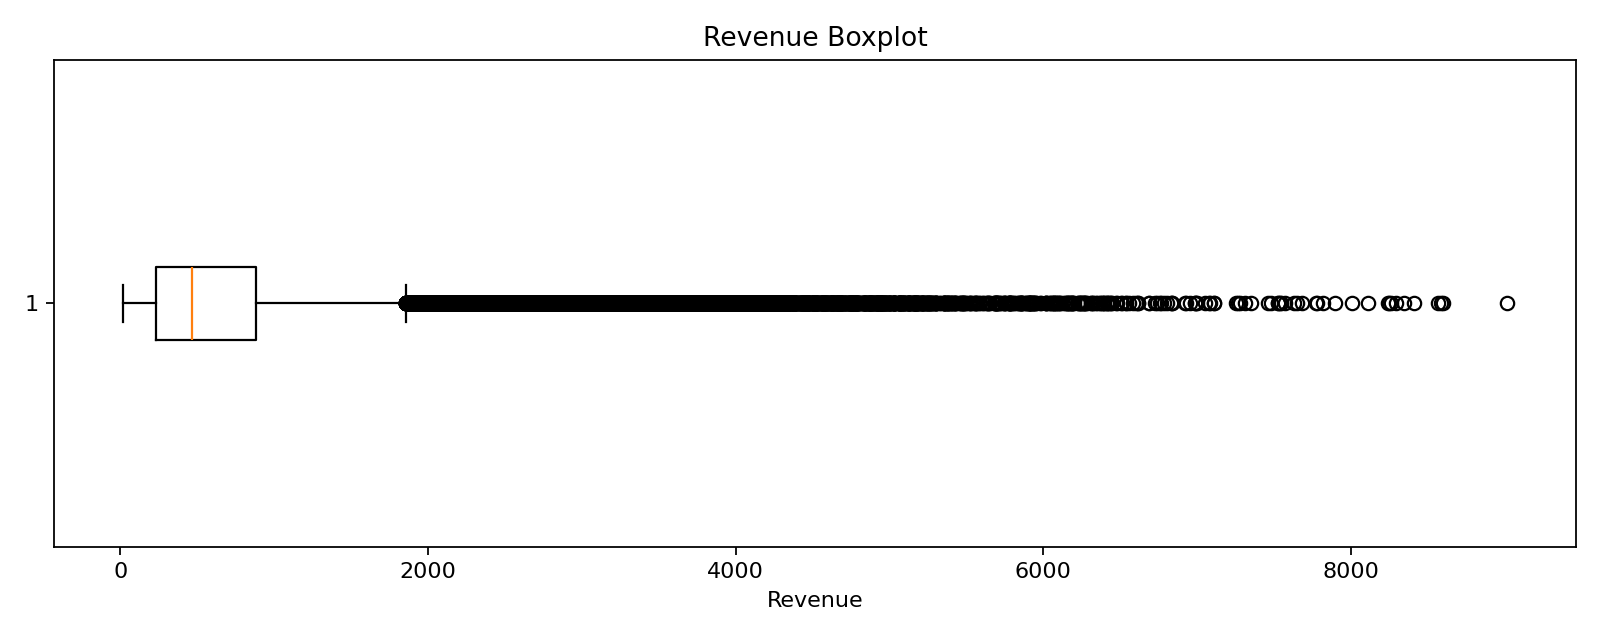
\includegraphics[width=\textwidth]{figures/lab02/revenue_boxplot.png}
  \caption{Revenue boxplot}
\end{figure}\
\vspace{4pt}
\begin{figure}[H]
  \centering
  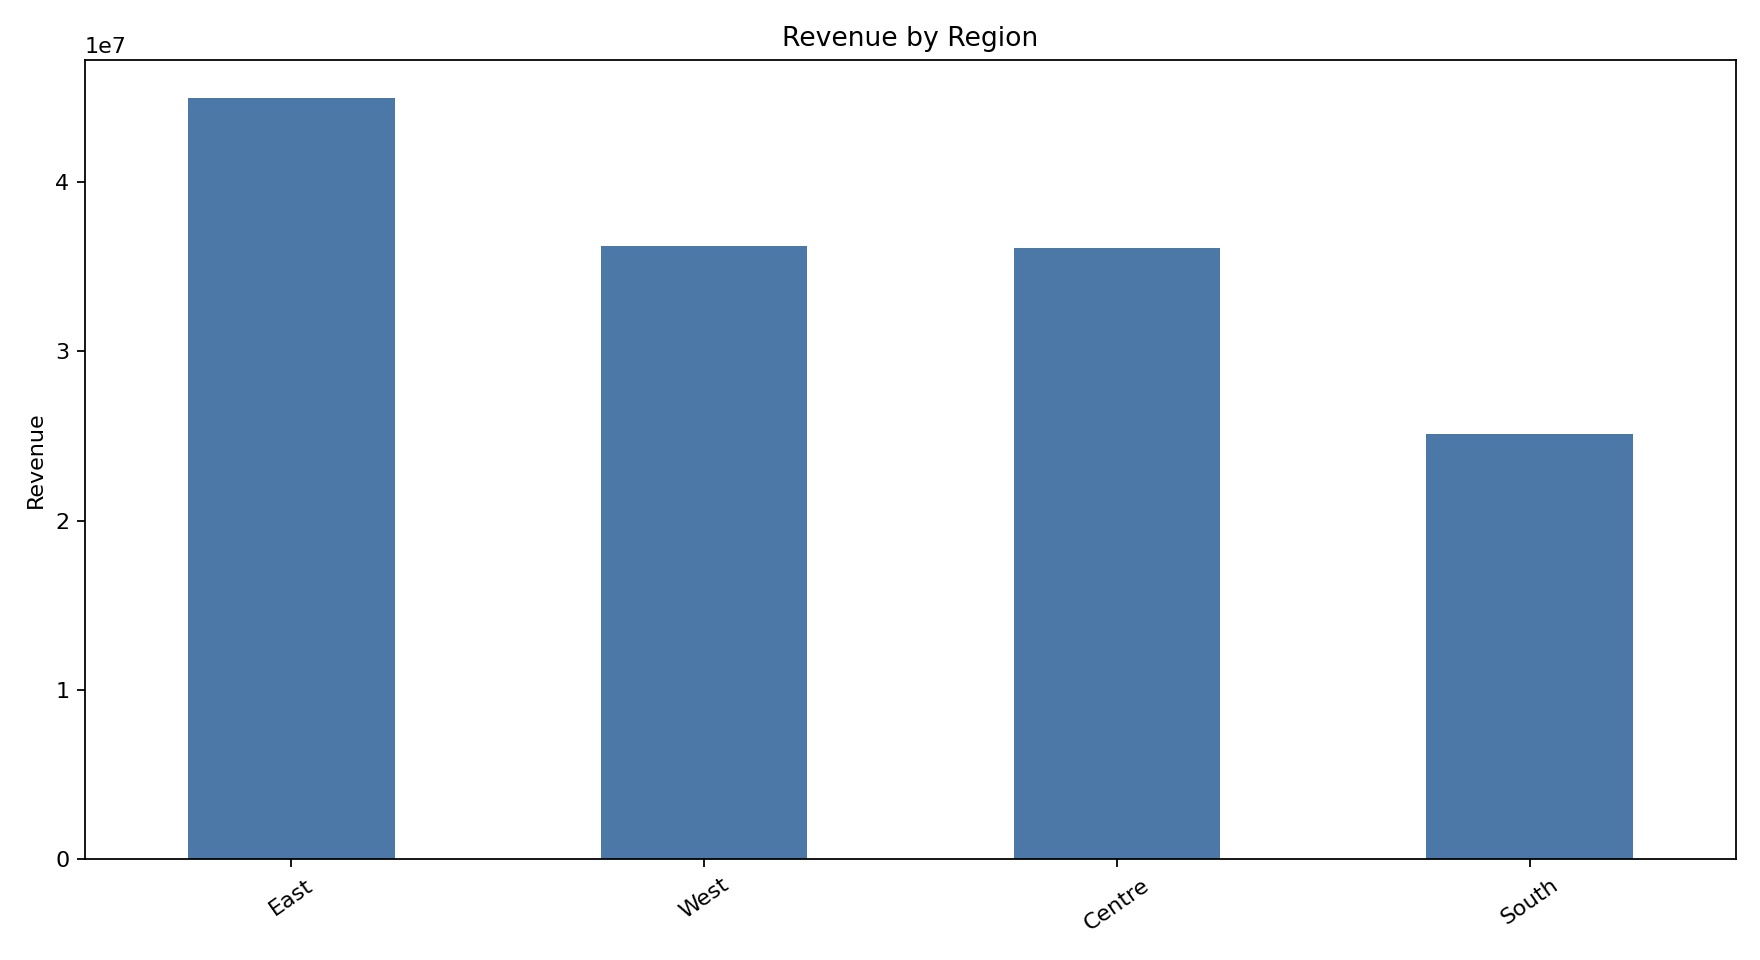
\includegraphics[width=\textwidth]{figures/lab02/revenue_by_region.png}
  \caption{Revenue by region}
\end{figure}
\begin{figure}[H]
  \centering
  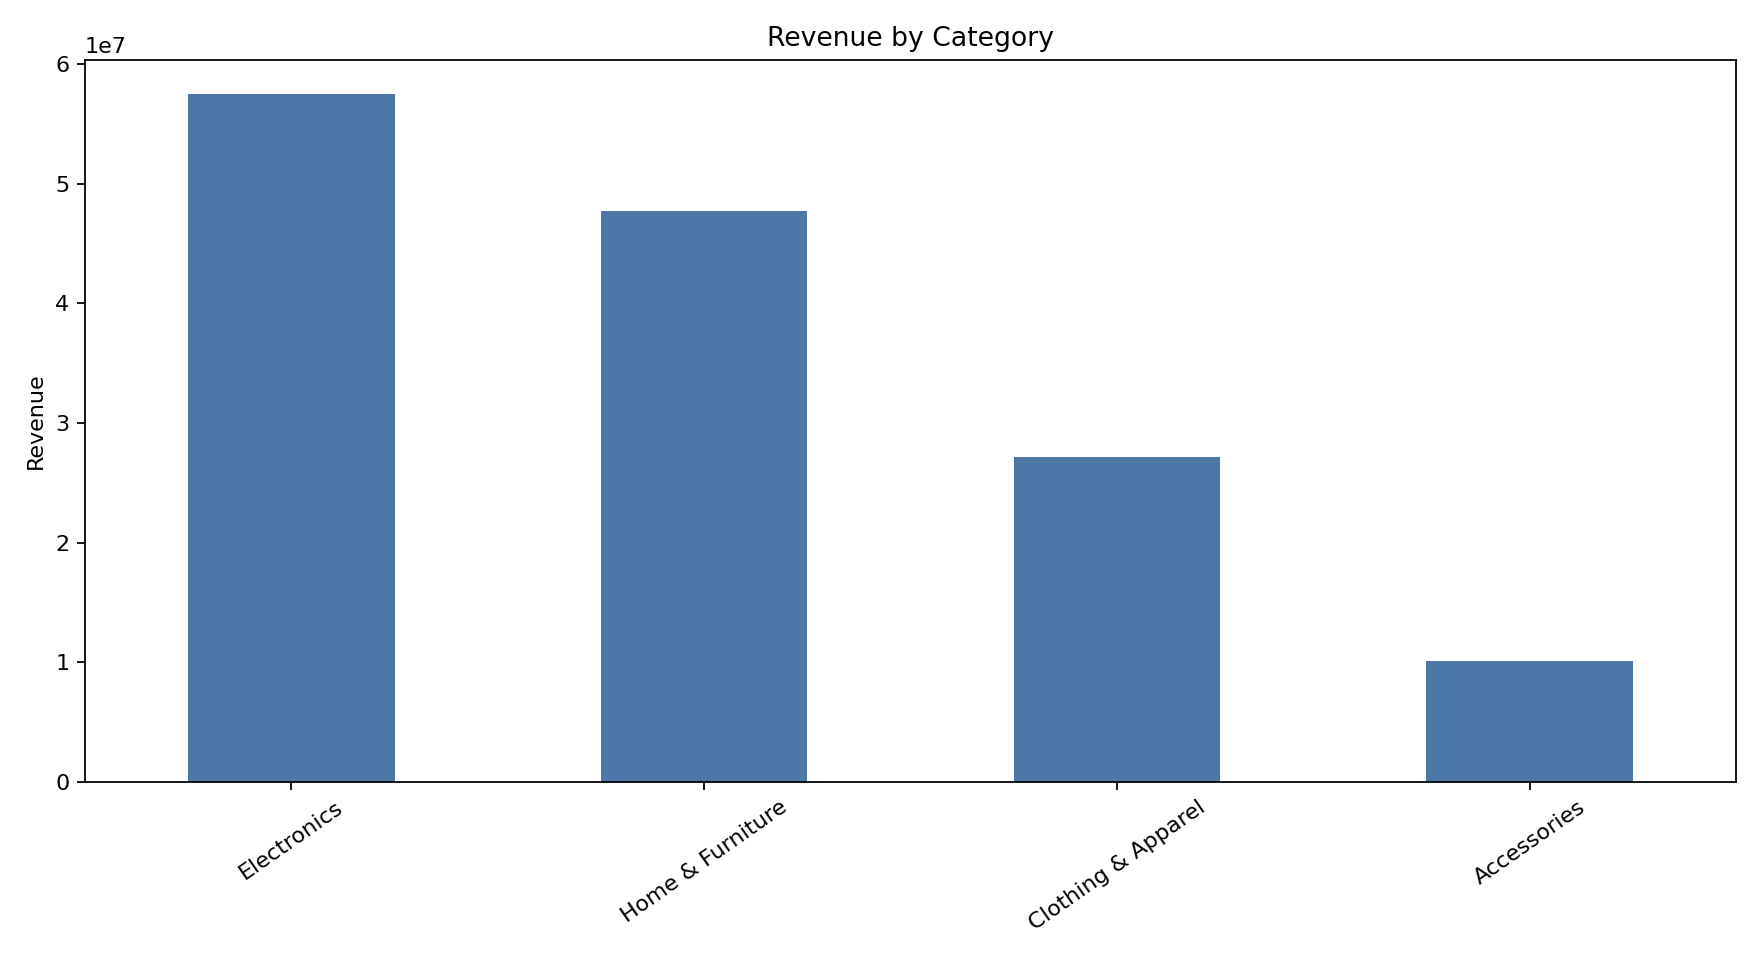
\includegraphics[width=\textwidth]{figures/lab02/revenue_by_category.png}
  \caption{Revenue by category}
\end{figure}\
\vspace{4pt}
\begin{figure}[H]
  \centering
  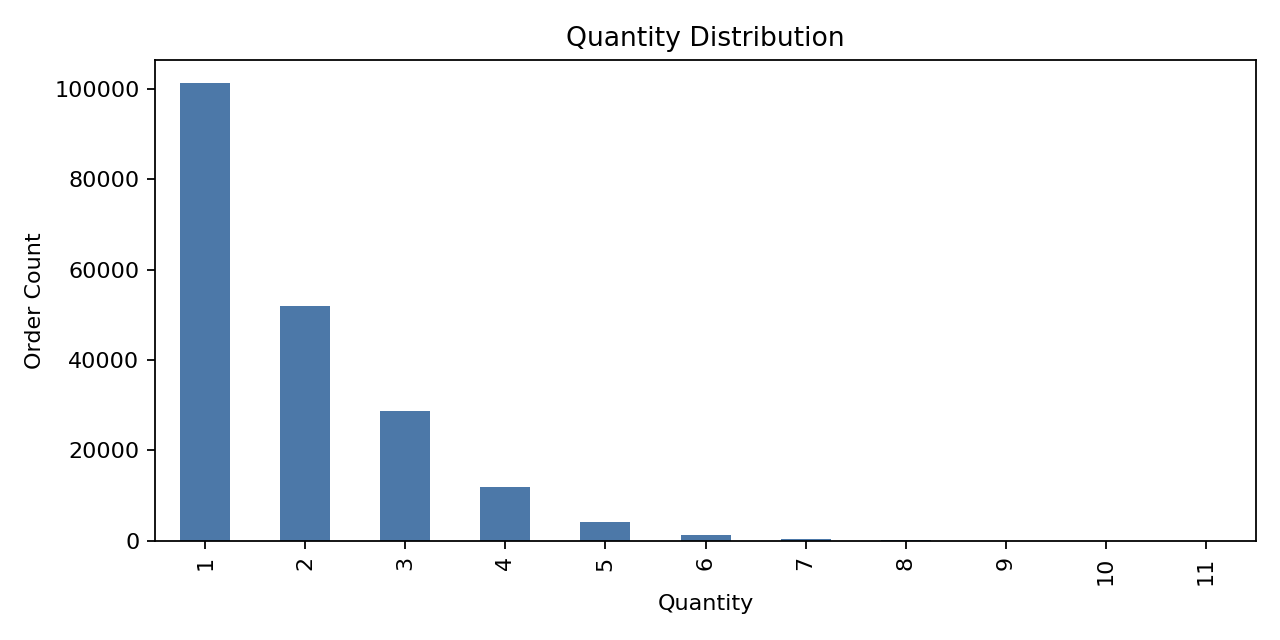
\includegraphics[width=\textwidth]{figures/lab02/quantity_distribution.png}
  \caption{Quantity distribution}
\end{figure}
\begin{figure}[H]
  \centering
  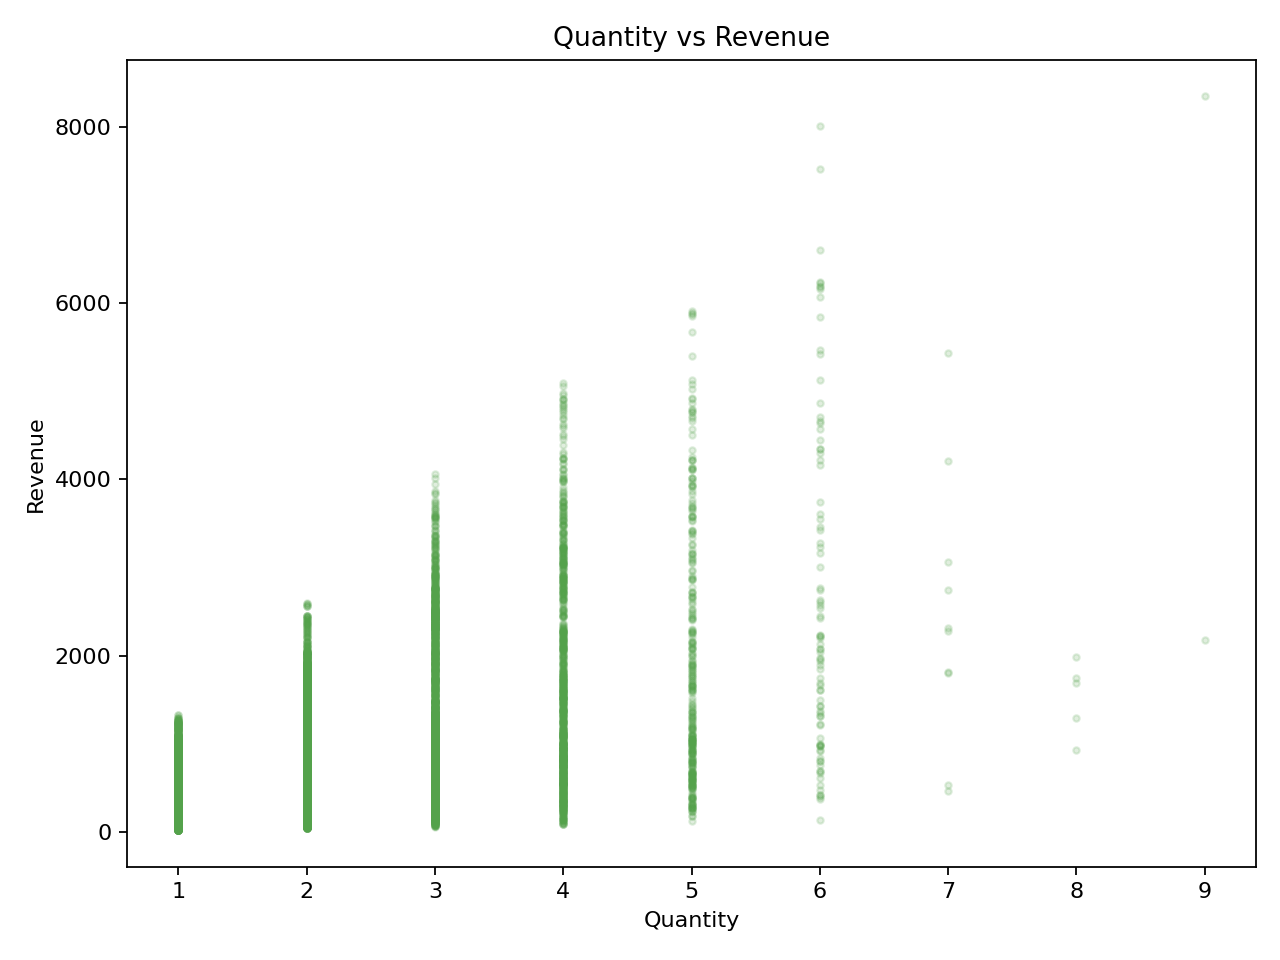
\includegraphics[width=\textwidth]{figures/lab02/quantity_vs_revenue.png}
  \caption{Quantity vs. revenue}
\end{figure}\
\vspace{4pt}
\begin{figure}[H]
  \centering
  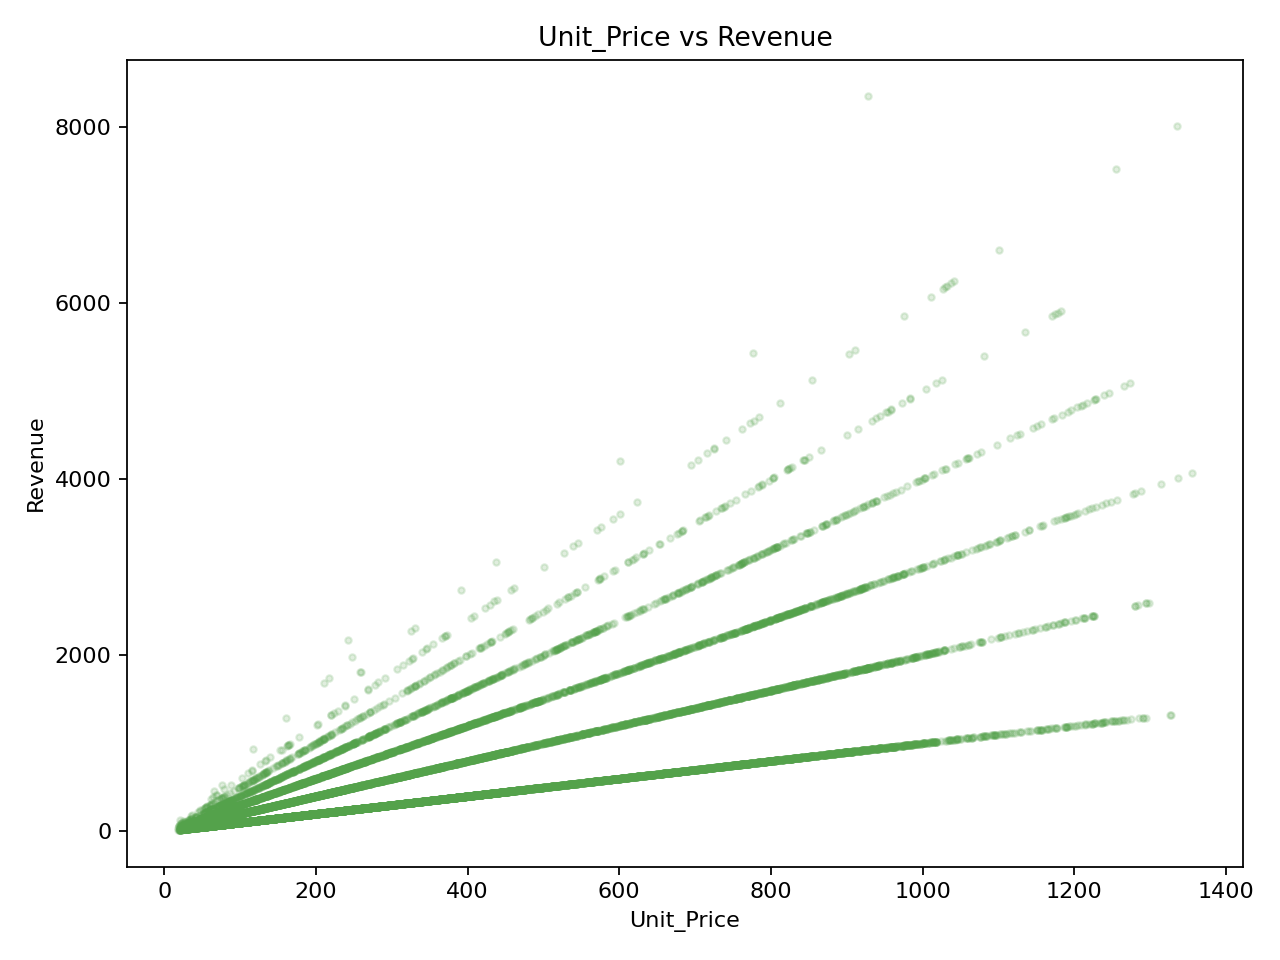
\includegraphics[width=\textwidth]{figures/lab02/unit_price_vs_revenue.png}
  \caption{Unit price vs. revenue}
\end{figure}
\begin{figure}[H]
  \centering
  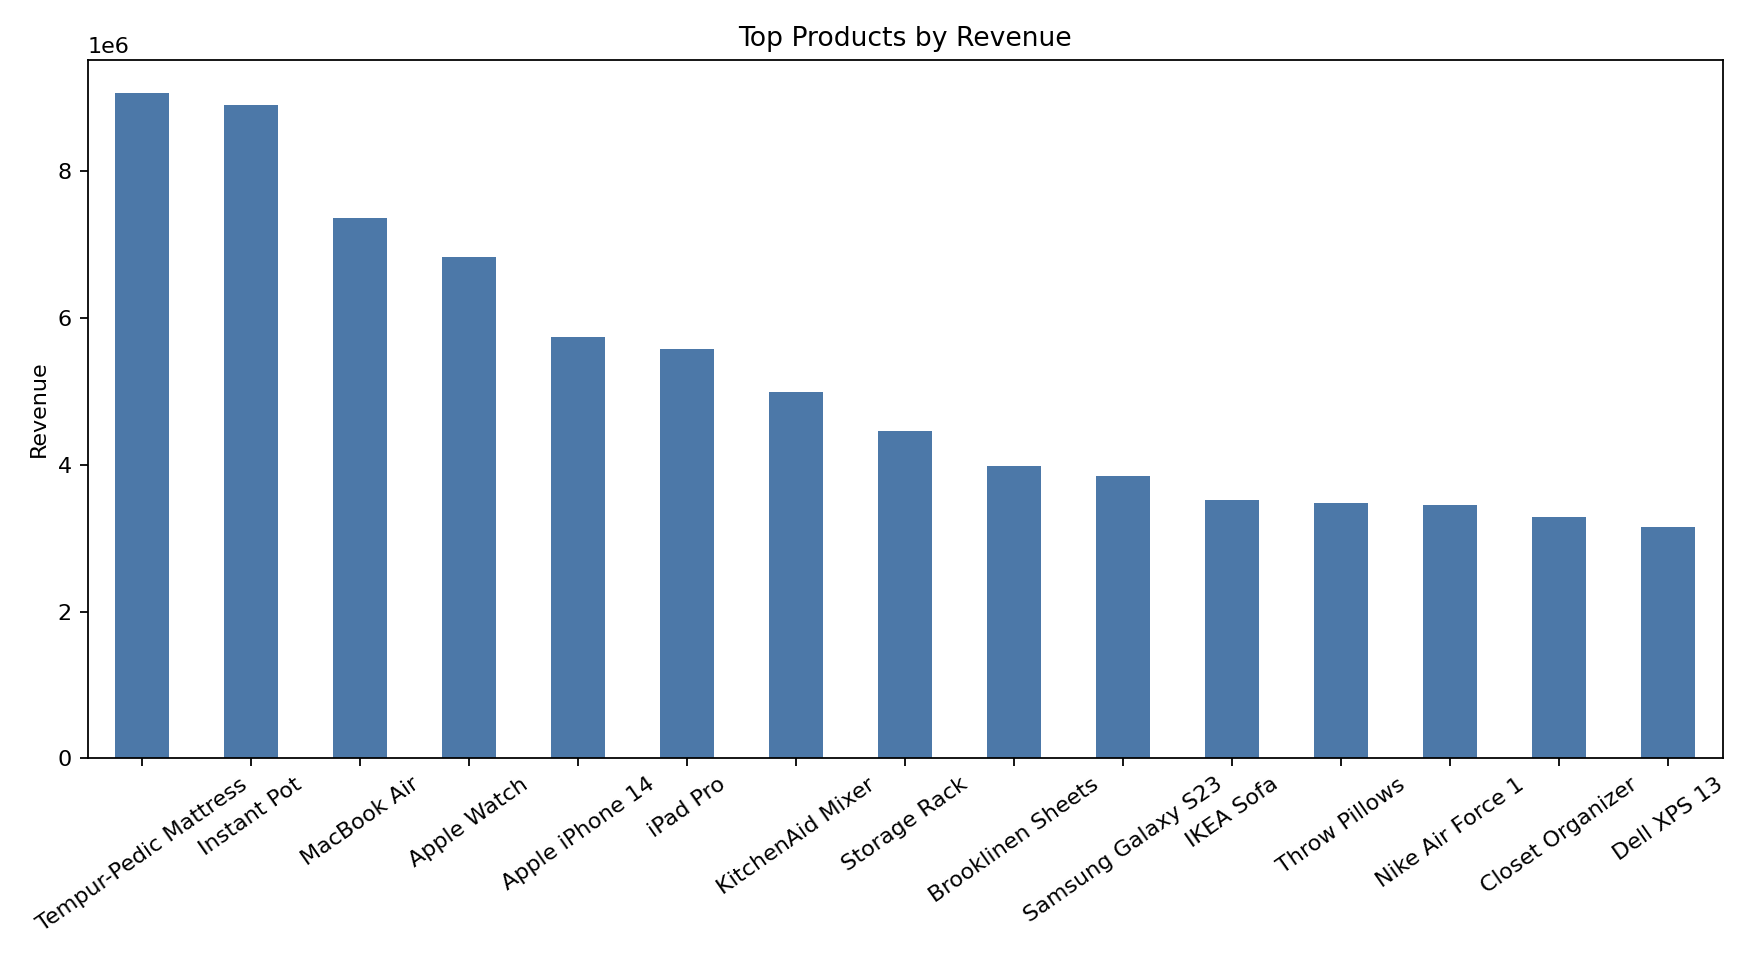
\includegraphics[width=\textwidth]{figures/lab02/top_products_by_revenue.png}
  \caption{Top products by revenue}
\end{figure}\
\vspace{4pt}
\begin{figure}[H]
  \centering
  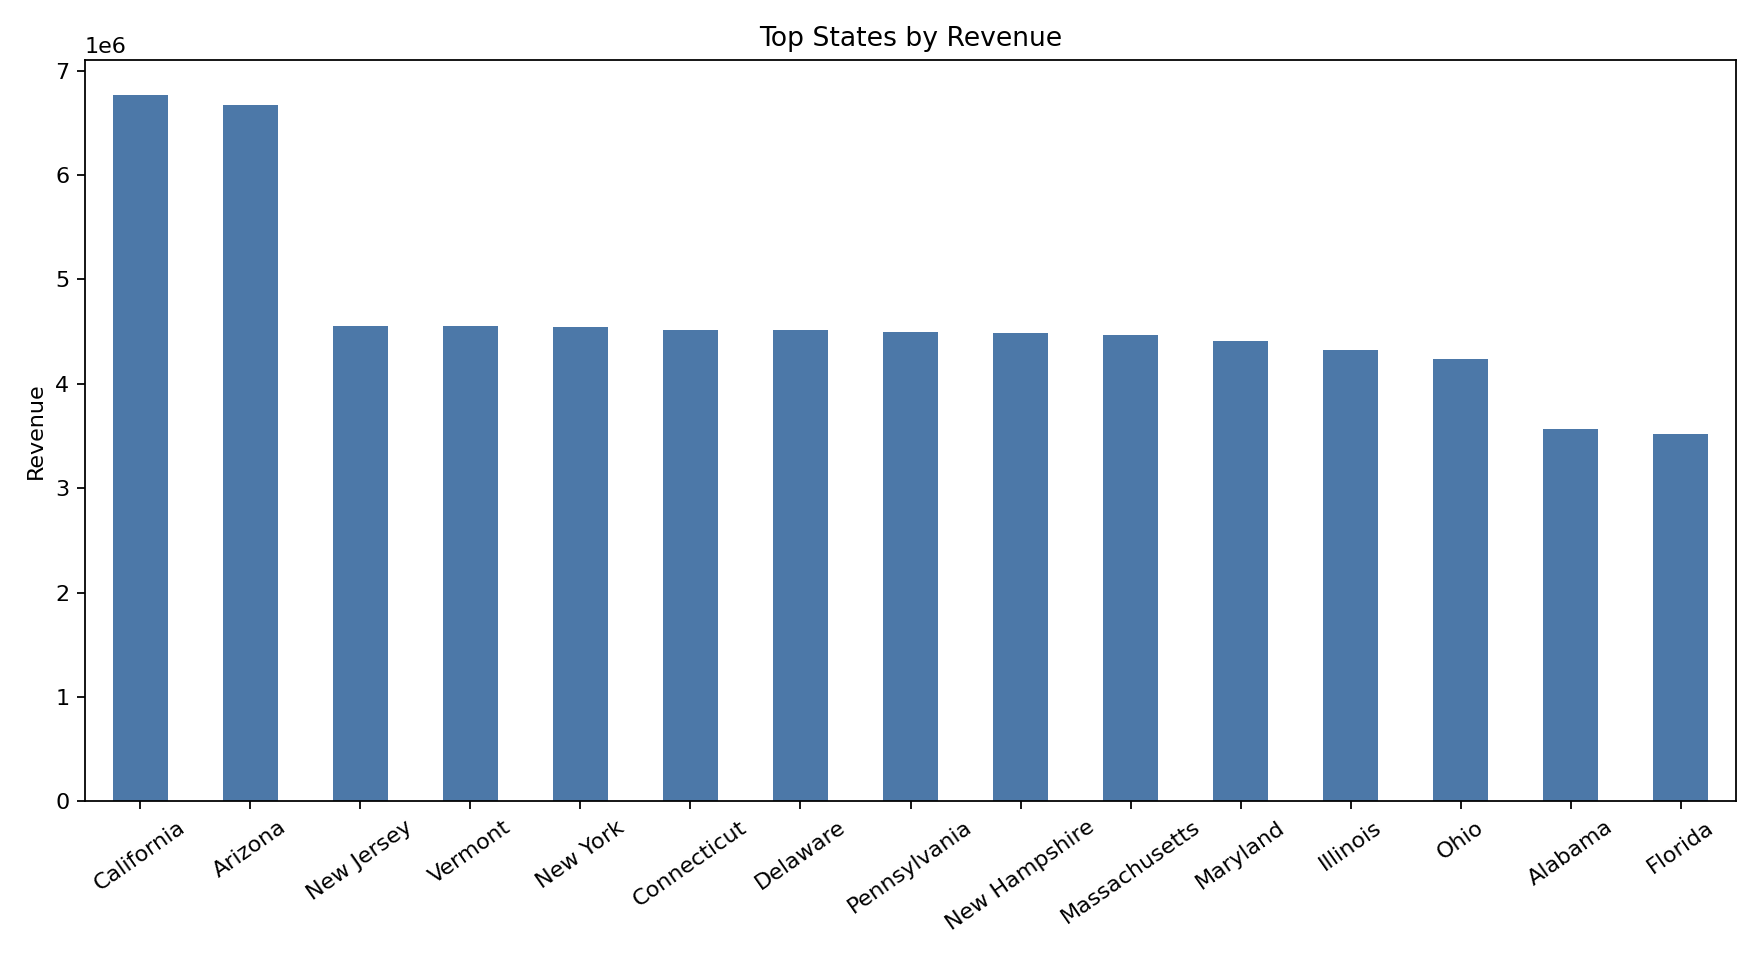
\includegraphics[width=0.48\textwidth]{figures/lab02/top_states_by_revenue.png}
  \caption{Top states by revenue}
\end{figure}
\end{figure}

\begin{notebox}
\textbf{HGB + Lag\_28 ensemble reduces RMSLE by 0.144 over the strong seasonal baseline.} The combination of boosting's non-linear pattern discovery with a seasonal baseline's stability is the key design pattern. Lag features consistently dominate feature importance — past sales are the strongest predictor of future sales. The 60/40 blend ratio balances pattern complexity against variance.
\end{notebox}

% ═══════════════════════════════════════════════════════════════
\chapter{Lab 03 — Customer Segmentation}
\label{ch:lab03}
% ═══════════════════════════════════════════════════════════════

\section{Problem Definition}

\begin{problembox}
Group mall customers into interpretable, actionable segments using \textbf{unsupervised clustering}. The goal is not to optimize a single metric, but to produce groups with clear behavioral signatures that a marketing team can immediately act upon. Success criteria: \textbf{silhouette score $> 0.30$}, clusters \textbf{$> 5$\% of total customers}, and semantically meaningful labels (e.g., ``High Income, High Spending'').
\end{problembox}

\subsection{Dataset}
\begin{itemize}
  \item \textbf{Source:} Shopping Mall Customer Segmentation Data (Kaggle), 15,079 rows.
  \item \textbf{Features:} \texttt{Age} (18–90), \texttt{Annual Income} (k\$), \texttt{Spending Score} (1–100), \texttt{Gender} (optional one-hot), \texttt{CustomerID} (excluded — it is a label, not a measurement).
  \item \textbf{Data quality:} No missing values, no duplicates — clean dataset.
\end{itemize}

\section{Complete Workflow}

\subsection{Step 0 — Reproducibility Setup}
A fixed random seed (42) ensures centroid initialization is deterministic across runs. Four local modules (\texttt{utils}, \texttt{preprocess}, \texttt{eda}, \texttt{clustering}) encapsulate logic; \texttt{importlib.reload()} enables code edits without kernel restart.

\subsection{Step 2 — Raw Data Overview}
\texttt{utils.find\_raw\_csv()} discovers the dataset via configurable glob pattern — no hardcoded filename. Column names are normalized to \texttt{customer\_id}, \texttt{gender}, \texttt{age}, \texttt{annual\_income}, \texttt{spending\_score} for consistent downstream access. The printed overview (shape, dtypes, missing, duplicates, descriptive stats) serves as the first quality checkpoint.

\subsection{Step 3 — Data Quality Checks}
Four issues are catalogued before any transformation:
\begin{itemize}
  \item \textbf{Missing values:} Per-column count and percentage.
  \item \textbf{Duplicates:} Exact row comparison. >1\% duplicates need investigation.
  \item \textbf{Invalid ranges:} Age 0–120, income $\ge$ 0, spending 1–100. Negative income or ages > 150 signal data corruption.
  \item \textbf{Outliers:} Both z-score ($|z| > 3$) and IQR ($Q1-1.5\times\text{IQR}$ to $Q3+1.5\times\text{IQR}$) methods. Outliers are summarized, \textbf{not removed} — the report quantifies deviations for informed case-by-case decisions.
\end{itemize}

The IQR method flags more points for right-skewed income data because it does not assume symmetry. A preprocessing report (markdown) is saved for audit trail.

\begin{figure}[H]\centering
\begin{figure}[H]
  \centering
  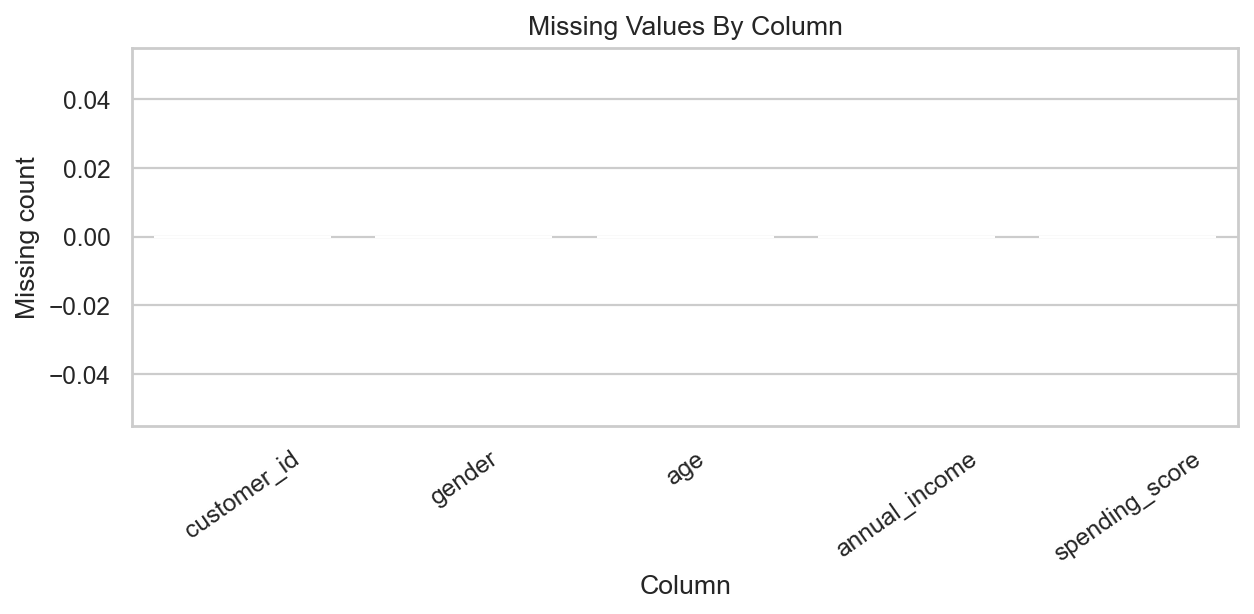
\includegraphics[width=\textwidth]{figures/lab03/missing_values.png}
  \caption{Missing values per column}
\end{figure}
\begin{figure}[H]
  \centering
  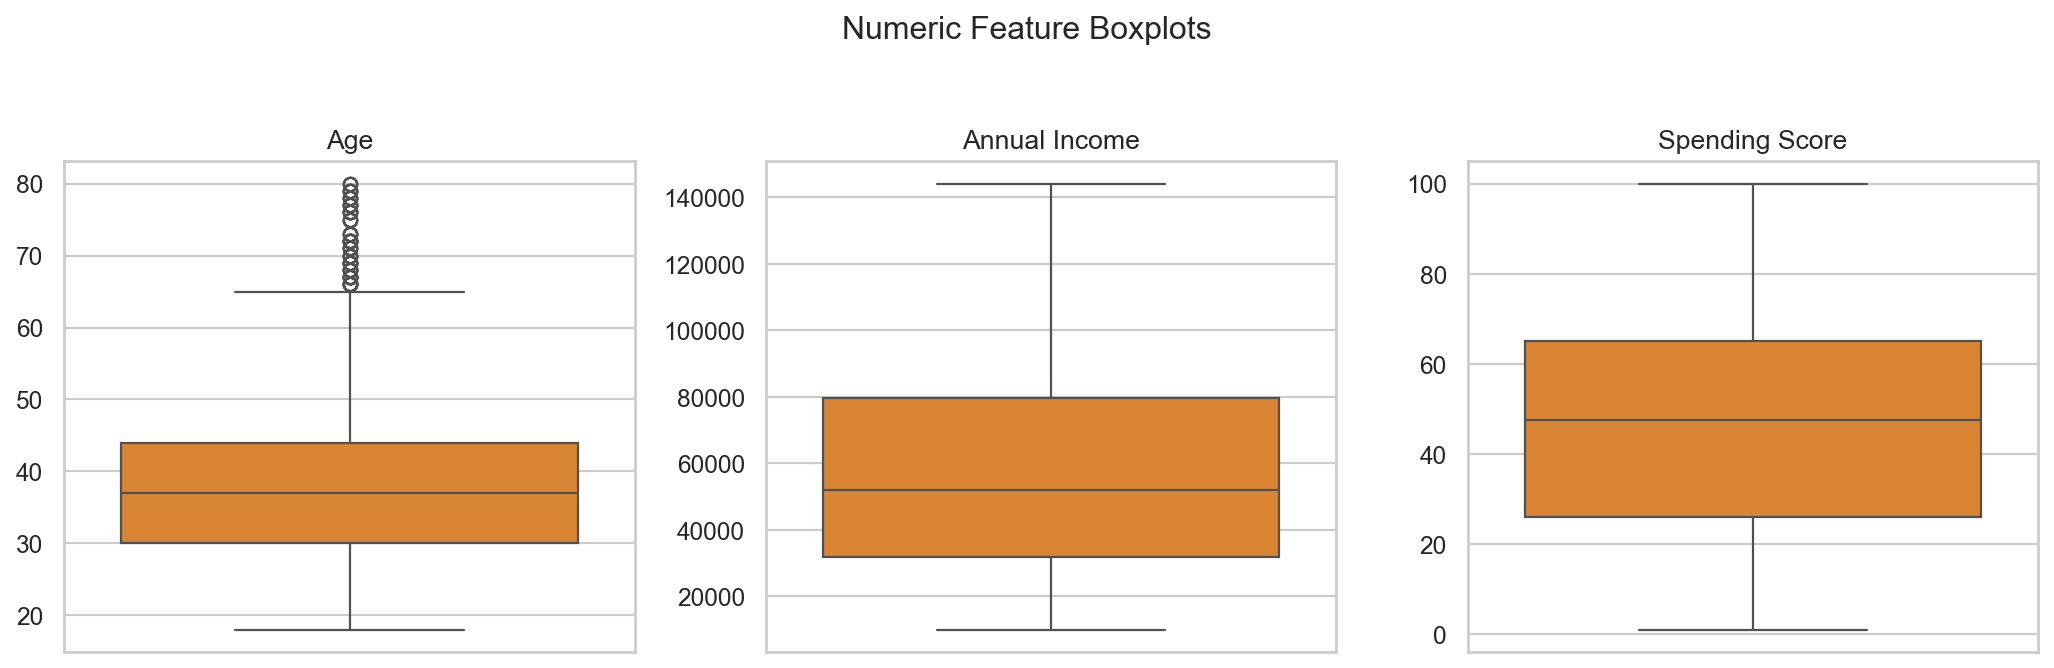
\includegraphics[width=\textwidth]{figures/lab03/boxplots_before.png}
  \caption{Boxplots: original scale outliers}
\end{figure}
\end{figure}

\begin{figure}[H]\centering
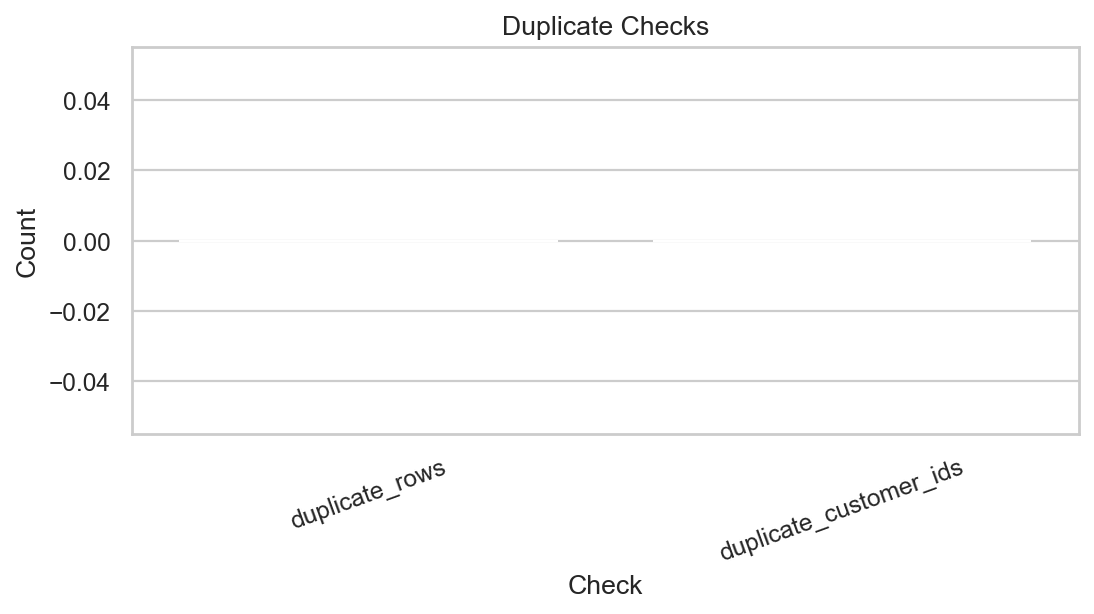
\includegraphics[width=0.7\textwidth]{figures/lab03/duplicate_summary.png}
\caption{Duplicate row summary — exact row matches and their distribution across columns.}
\end{figure}

\subsection{Step 4 — EDA Before Preprocessing}

EDA runs in \textbf{original units} — before scaling abstracts the numbers away. Six plots cover the full picture:

\begin{table}[H]
\centering\rowcolors{2}{tablerow}{white}
\begin{tabular}{l L{8cm}}
\toprule\rowcolor{tablehead!80}\color{white}\textbf{Plot} &\color{white}\textbf{Key Question}\\
\midrule
Histograms/KDE & Are age, income, spending uniformly distributed? Bimodal spending suggests natural clusters.\\
Gender distribution & Is the customer base balanced? A skew > 70/30 should be noted.\\
Income vs. Spending scatter & \textbf{Most important plot.} Do 4–6 visually separable clouds appear? If yes, clustering will succeed.\\
Age vs. Spending scatter & Does age predict spending? A downward trend is actionable for age-targeted campaigns.\\
Age vs. Income scatter & Are older customers wealthier?\\
Correlation heatmap & Any $|r| > 0.7$ indicates redundant features that can be dropped.\\
Pairplot & All pairwise scatters in one grid — catches interactions a correlation coefficient would miss.\\
\bottomrule
\end{tabular}
\caption{EDA before preprocessing — 6 diagnostic views}
\end{table}

The \textbf{Income vs. Spending scatter} is the most important plot in the entire notebook. The classic Mall Customers dataset typically shows \textbf{5 distinct clusters}: high/high, high/low, medium/medium, low/high, low/low.

\begin{figure}[H]\centering
\begin{figure}[H]
  \centering
  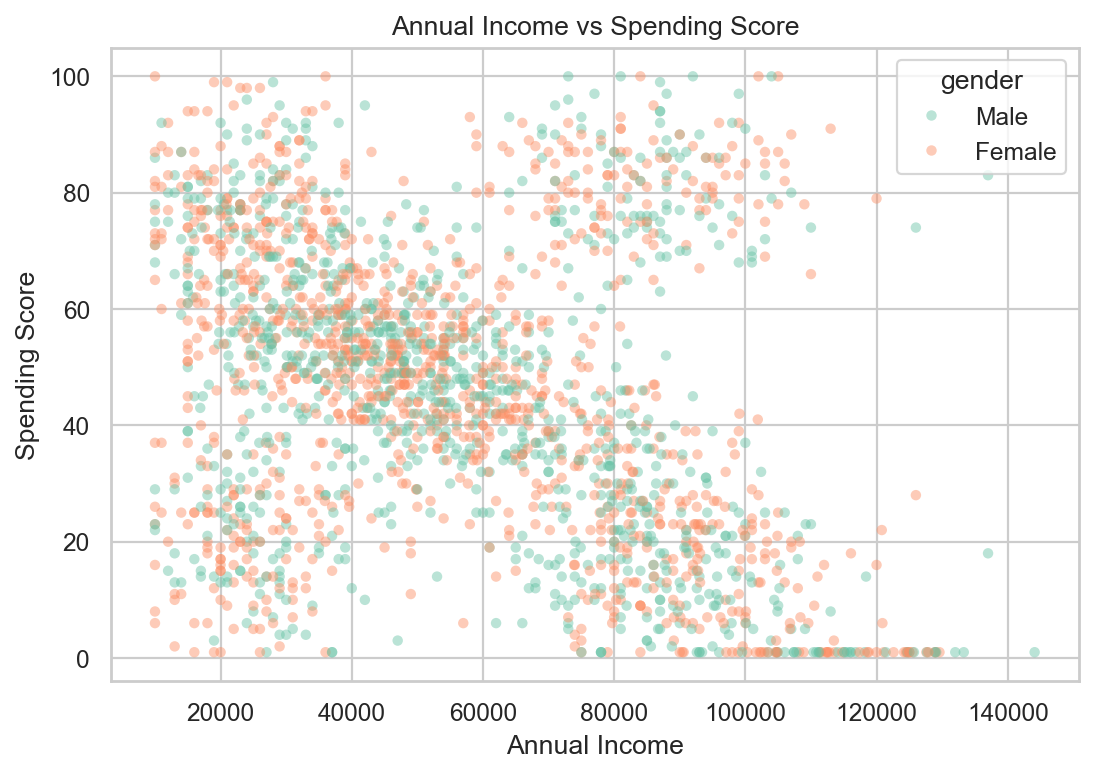
\includegraphics[width=\textwidth]{figures/lab03/scatter_annual_income_vs_spending_score_before.png}
  \caption{Income vs. Spending Score}
\end{figure}
\begin{figure}[H]
  \centering
  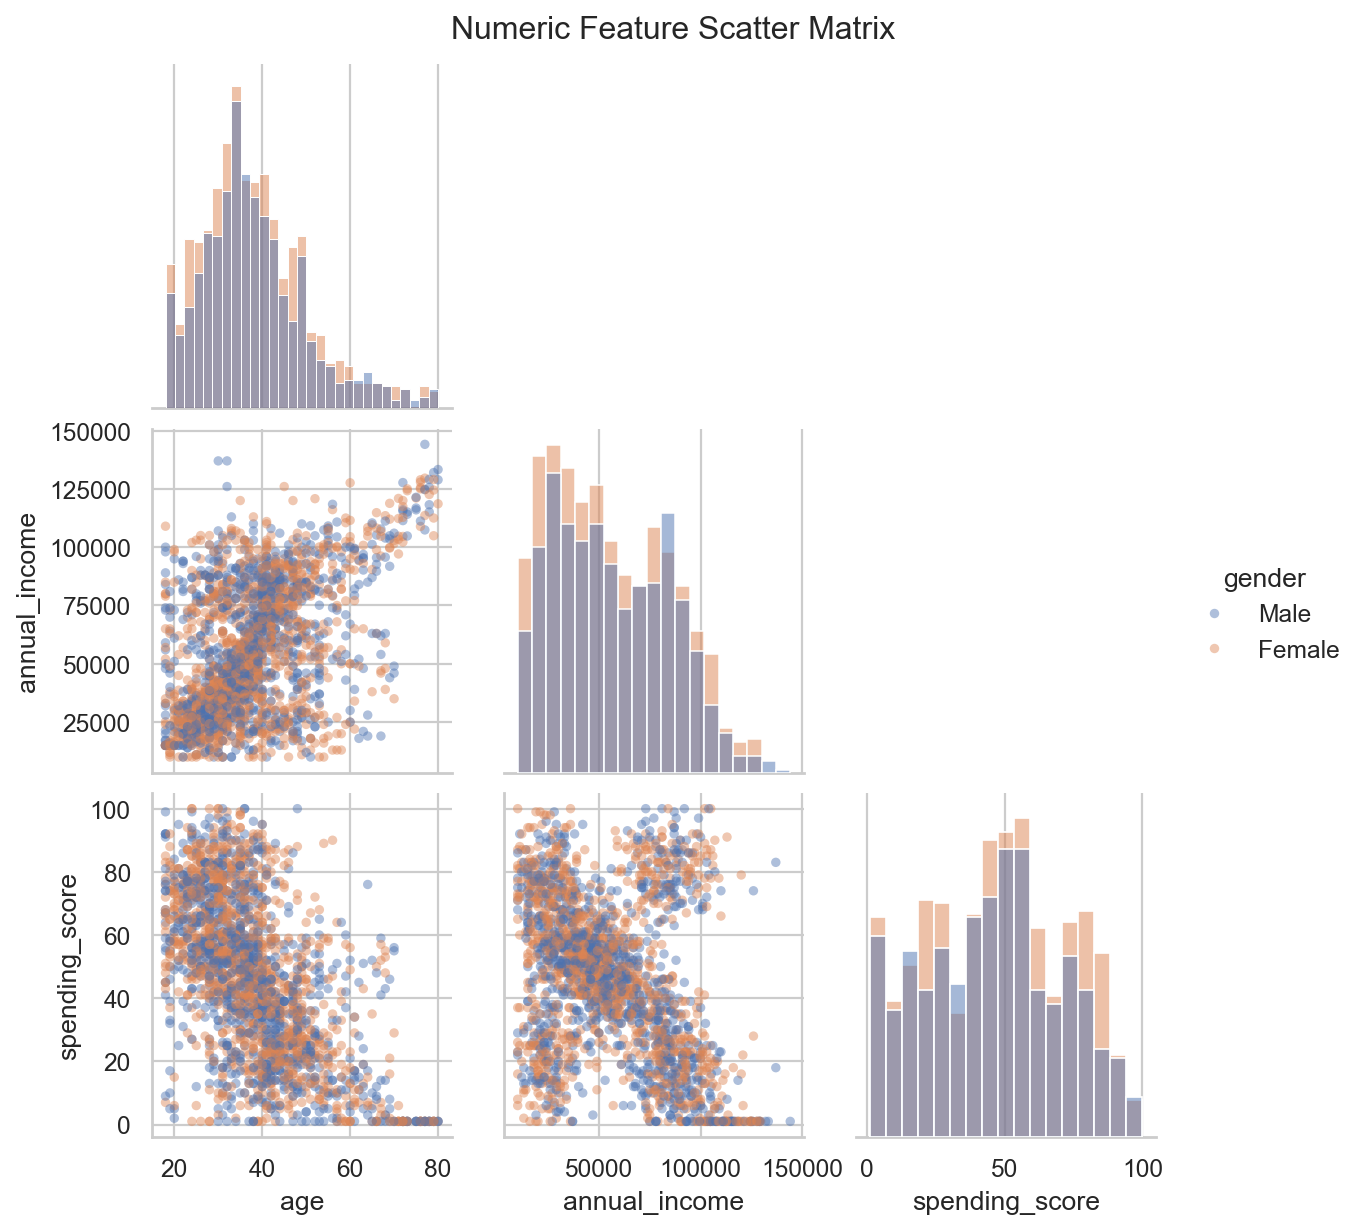
\includegraphics[width=\textwidth]{figures/lab03/pairplot_before.png}
  \caption{Pairwise scatter matrix}
\end{figure}
\end{figure}

\begin{figure}[H]\centering
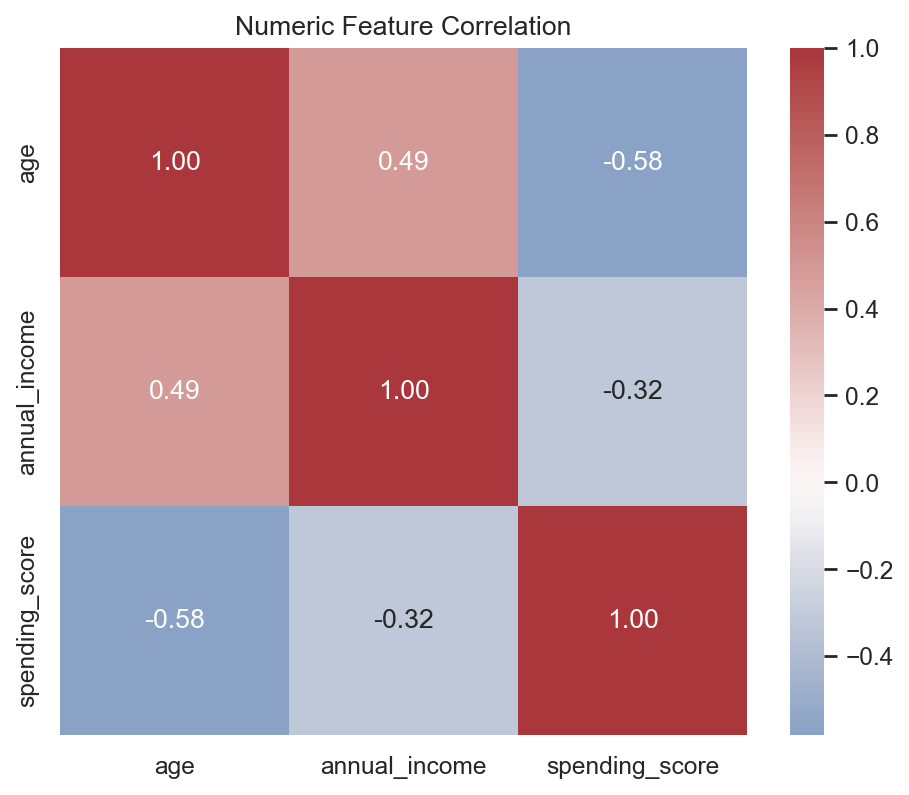
\includegraphics[width=0.8\textwidth]{figures/lab03/correlation_heatmap_before.png}
\caption{Correlation heatmap — no $|r| > 0.7$ redundancies, confirming all features contribute independent information.}
\end{figure}

\begin{figure}[H]\centering
\begin{figure}[H]
  \centering
  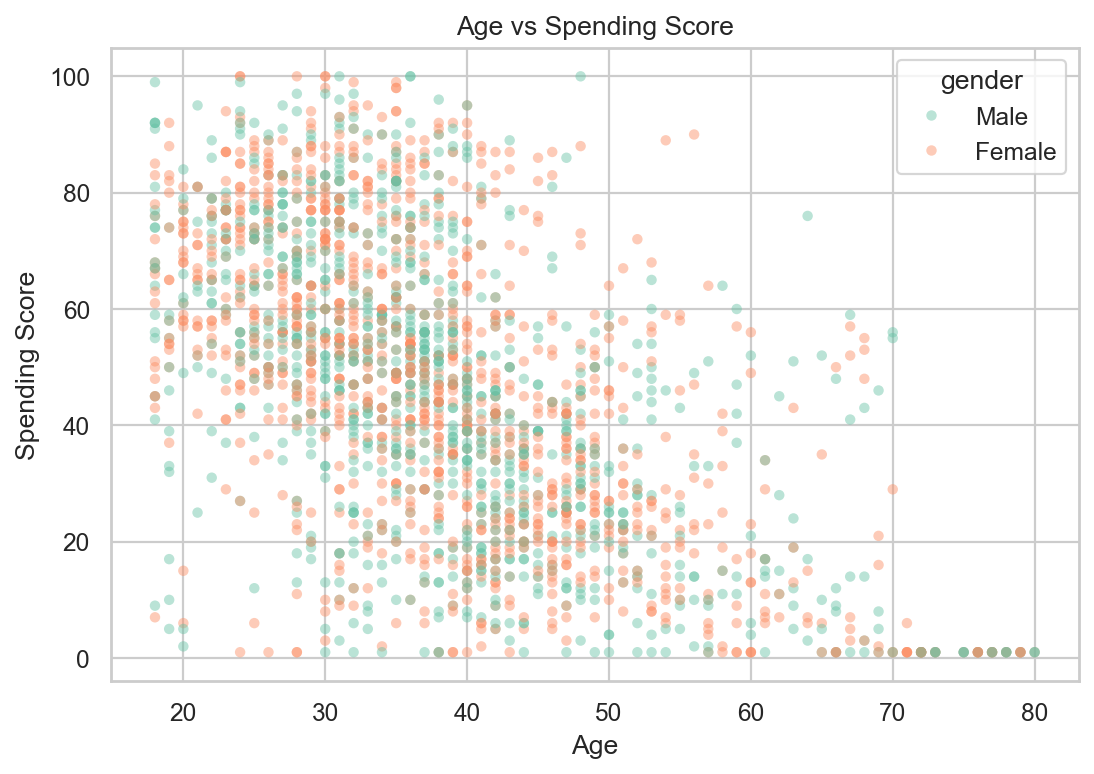
\includegraphics[width=\textwidth]{figures/lab03/scatter_age_vs_spending_score_before.png}
  \caption{Age vs. Spending Score}
\end{figure}
\begin{figure}[H]
  \centering
  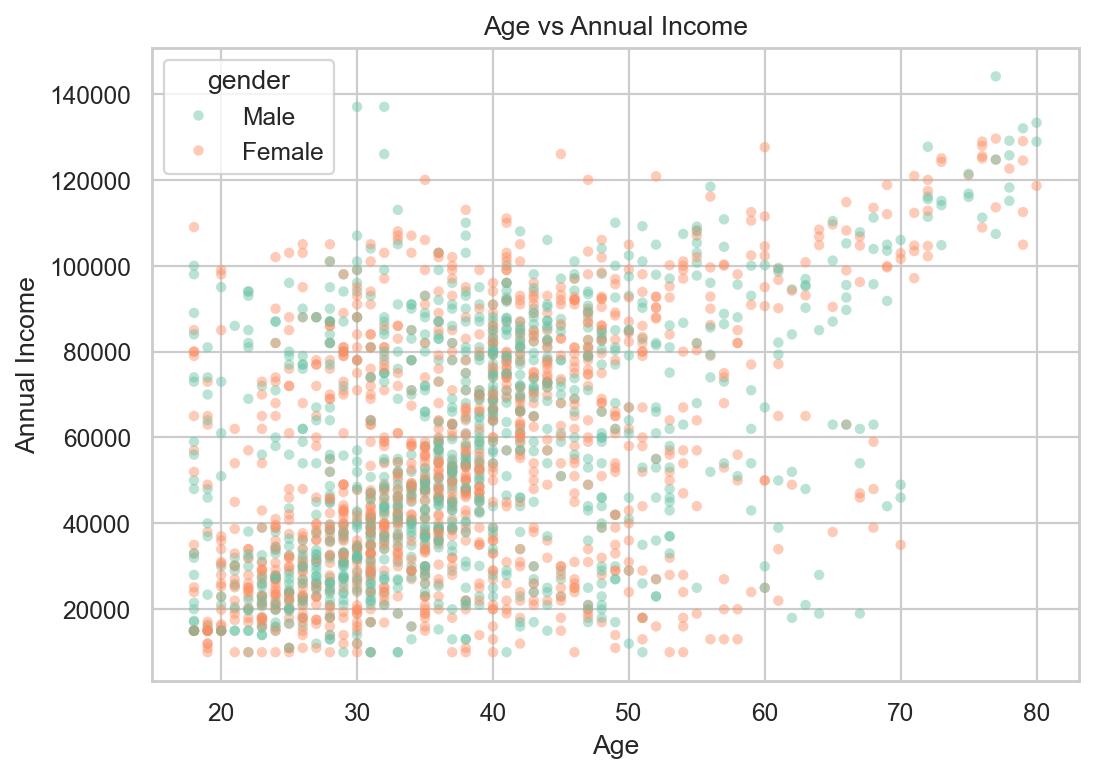
\includegraphics[width=\textwidth]{figures/lab03/scatter_age_vs_annual_income_before.png}
  \caption{Age vs. Annual Income}
\end{figure}
\end{figure}

\begin{figure}[H]\centering
\begin{figure}[H]
  \centering
  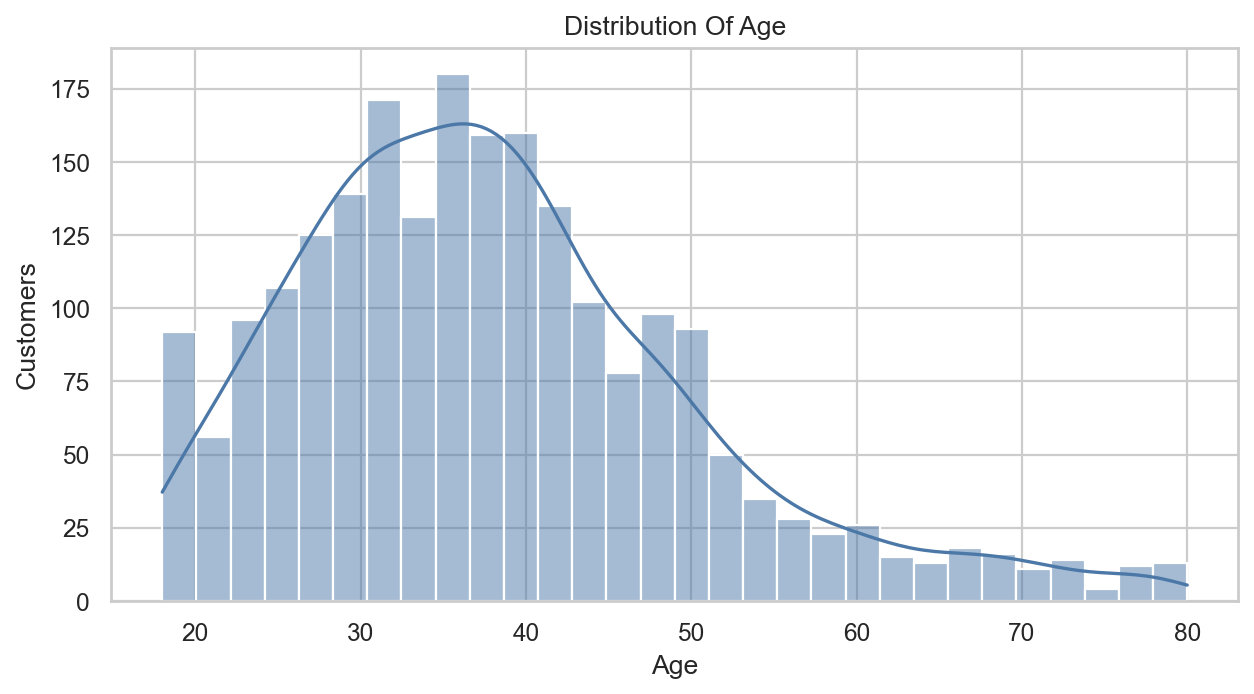
\includegraphics[width=\textwidth]{figures/lab03/distribution_age_before.png}
  \caption{Age distribution}
\end{figure}
\begin{figure}[H]
  \centering
  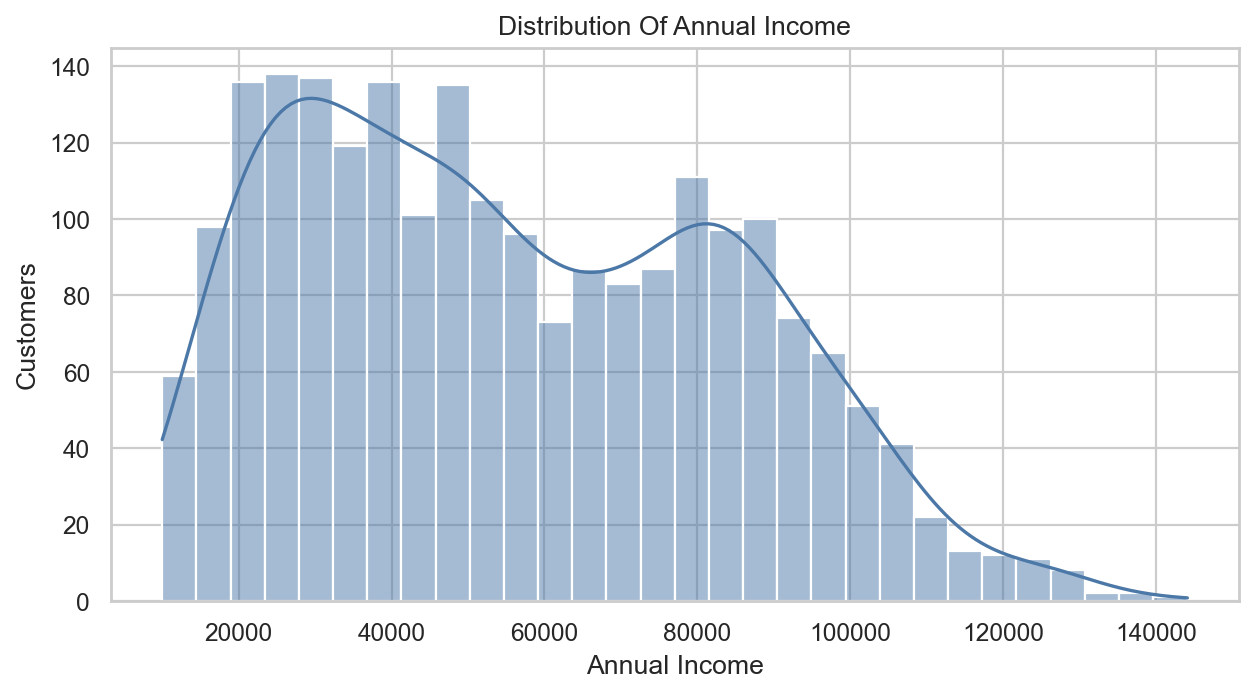
\includegraphics[width=\textwidth]{figures/lab03/distribution_annual_income_before.png}
  \caption{Annual income distribution}
\end{figure}
\begin{figure}[H]
  \centering
  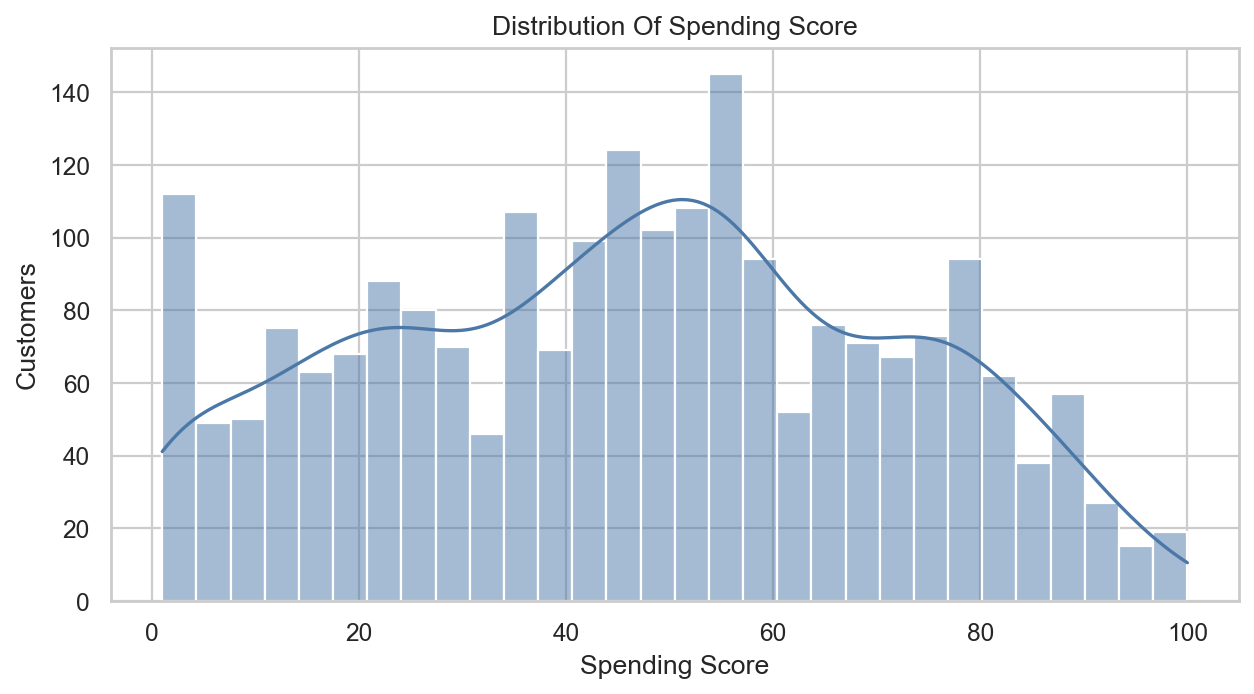
\includegraphics[width=\textwidth]{figures/lab03/distribution_spending_score_before.png}
  \caption{Spending score distribution}
\end{figure}
\end{figure}

\begin{figure}[H]\centering
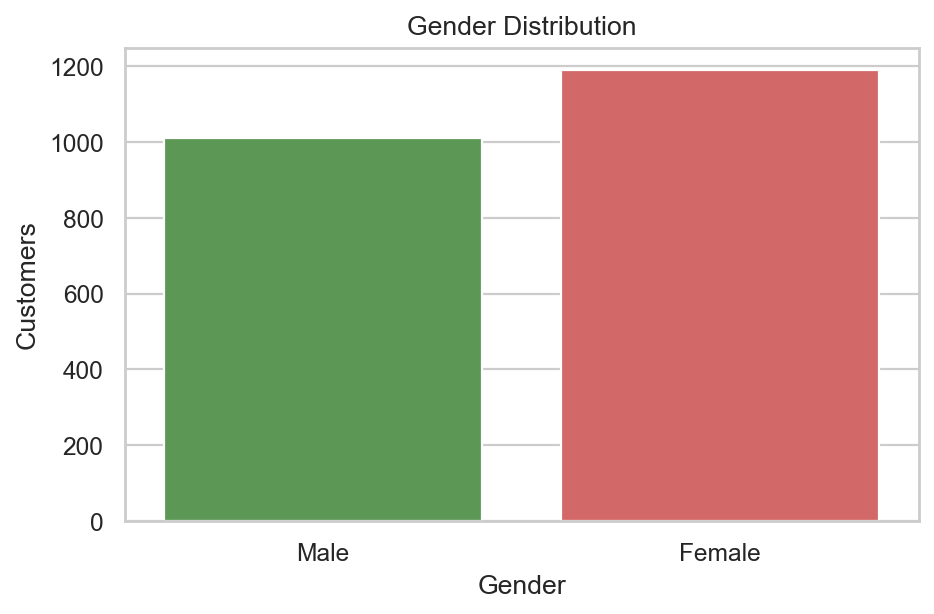
\includegraphics[width=0.6\textwidth]{figures/lab03/gender_distribution_before.png}
\caption{Gender distribution — note any imbalance that may affect segment interpretation.}
\end{figure}

\subsection{Step 5 — Preprocessing and Feature Scaling}

Without scaling, distance-based clustering is dominated by the feature with the largest scale. For this dataset, \texttt{annual\_income} (15–137) would dominate \texttt{age} (18–70) by an order of magnitude. Three scalers are compared:

\begin{table}[H]
\centering\rowcolors{2}{tablerow}{white}
\begin{tabular}{l L{4cm} L{4cm} L{4cm}}
\toprule\rowcolor{tablehead!80}\color{white}\textbf{Scaler} &\color{white}\textbf{Transform} &\color{white}\textbf{Best when} &\color{white}\textbf{Risk}\\
\midrule
Standard & $z = (x-\mu)/\sigma$ & Symmetric features, no extreme outliers & Outliers distort $\mu$ and $\sigma$\\
MinMax & $x' = (x-\min)/(\max-\min)$ & Bounded [0,1] needed, no outliers & One extreme value compresses all others\\
Robust & $x' = (x-\text{median})/\text{IQR}$ & Heavy outliers, skewed data & Less common in clustering literature\\
\bottomrule
\end{tabular}
\caption{Scaler comparison for clustering}
\end{table}

Four feature sets are tested, creating a \textbf{preprocessing grid}:
\begin{itemize}
  \item \texttt{behavior\_numeric} — age, income, spending (primary baseline).
  \item \texttt{income\_spending\_only} — the two most business-relevant dimensions.
  \item \texttt{age\_spending\_only} — tests whether age alone segments spending.
  \item \texttt{behavior\_plus\_gender} — adds one-hot encoded gender; if it doesn't improve silhouette, exclude for simplicity.
\end{itemize}

\subsection{Step 6 — Clustering Experiments}

A grid search runs K-Means ($K=2..10$) and Gaussian Mixture Model on selected configurations:

\begin{table}[H]
\centering\rowcolors{2}{tablerow}{white}
\begin{tabular}{l L{5cm} L{5cm}}
\toprule\rowcolor{tablehead!80}\color{white}\textbf{Algorithm} &\color{white}\textbf{Strengths} &\color{white}\textbf{Weaknesses}\\
\midrule
K-Means & Fast, interpretable, well-suited for spherical clusters & Assumes equal cluster size, spherical shape\\
GMM & Soft assignments, handles elliptical clusters, expresses uncertainty & More parameters, sensitive to initialization, slower\\
\bottomrule
\end{tabular}
\caption{Clustering algorithms evaluated}
\end{table}

Four metrics are tracked for every configuration:

\begin{table}[H]
\centering\rowcolors{2}{tablerow}{white}
\begin{tabular}{l c L{5cm}}
\toprule\rowcolor{tablehead!80}\color{white}\textbf{Metric} &\color{white}\textbf{Direction} &\color{white}\textbf{What it measures}\\
\midrule
Inertia & $\downarrow$ & Within-cluster sum of squares — always decreases with K; use only for elbow\\
Silhouette & $\uparrow$ & Compactness $\times$ separation; range $[-1, +1]$\\
Calinski-Harabasz & $\uparrow$ & Between-cluster vs. within-cluster variance ratio\\
Davies-Bouldin & $\downarrow$ & Average similarity between each cluster and its nearest neighbor\\
\bottomrule
\end{tabular}
\caption{Four complementary clustering metrics}
\end{table}

A \textbf{verification cell} runs both scratch and library implementations on a 100-sample subset, using the \textbf{Hungarian algorithm} (linear sum assignment) to align cluster labels. A partition match rate $> 90\%$ confirms correctness. The same verification is applied to GMM with relaxed tolerance.

\begin{figure}[H]\centering
\begin{figure}[H]
  \centering
  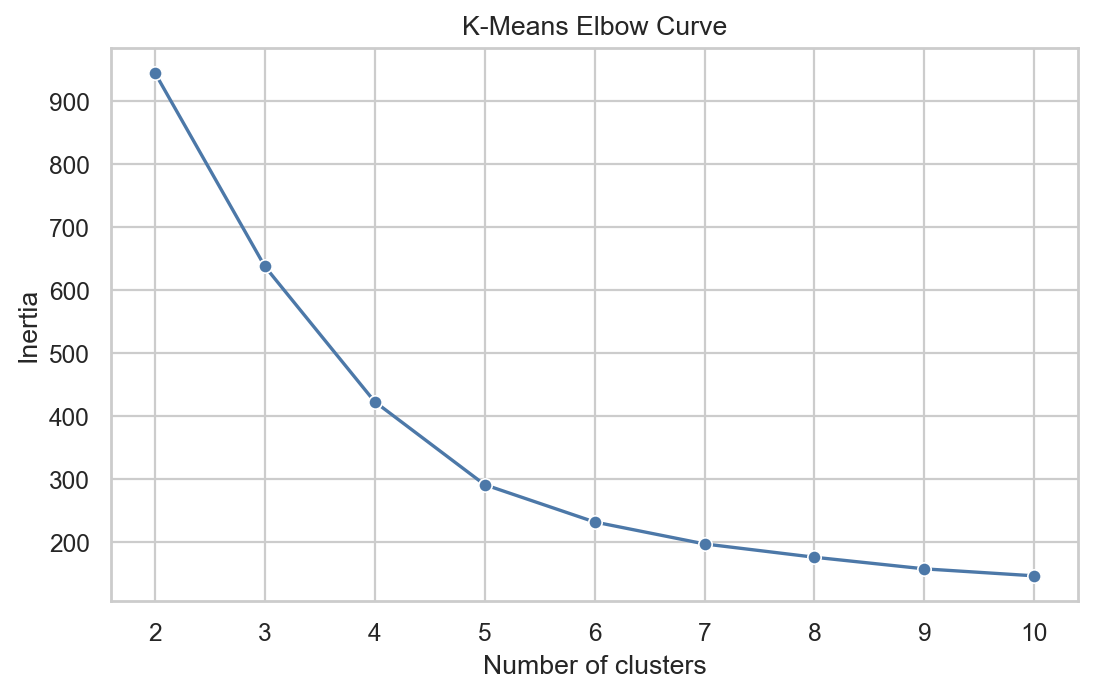
\includegraphics[width=\textwidth]{figures/lab03/kmeans_elbow_curve.png}
  \caption{Elbow curve — bend at K=3–5}
\end{figure}
\begin{figure}[H]
  \centering
  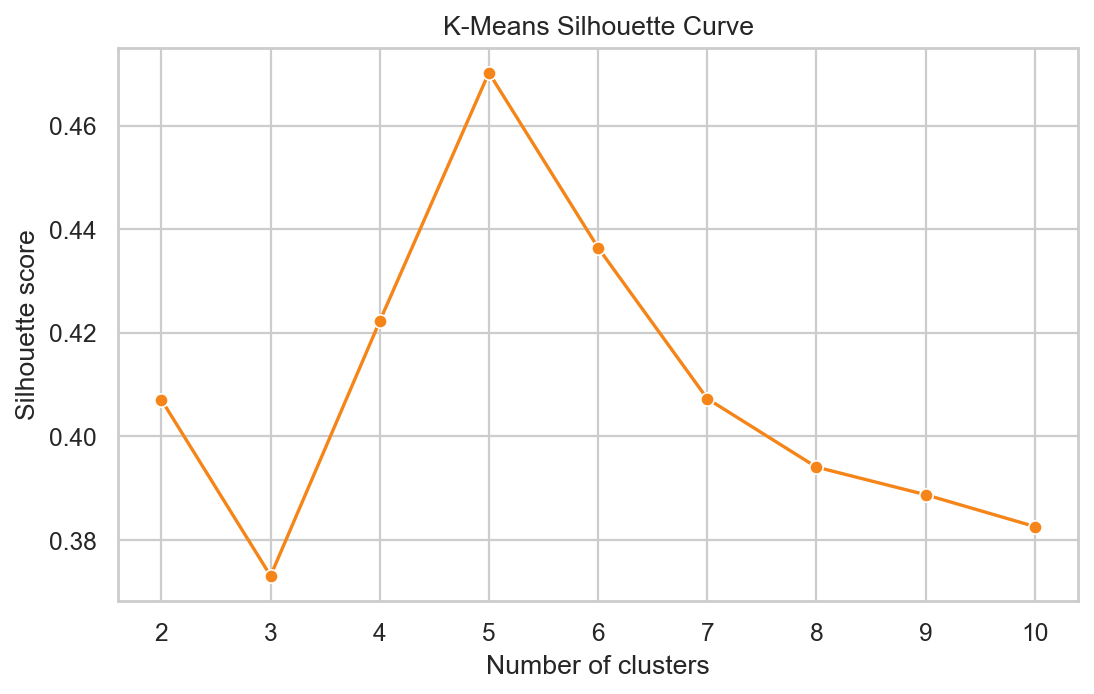
\includegraphics[width=\textwidth]{figures/lab03/kmeans_silhouette_curve.png}
  \caption{Silhouette vs. K — peak at 5 clusters}
\end{figure}
\end{figure}

\subsubsection{K-Means From Scratch — Core Implementation}

The implementation includes \textbf{k-means++ initialization} (spreading initial centroids to avoid poor local minima) and \textbf{multi-start} ($\text{n\_init}=10$) with the best inertia kept:

\begin{pythoncode}[caption={K-Means: k-means++ init + assignment-update loop}]
# k-means++ initialization
centers = np.zeros((n_clusters, n_features))
centers[0] = X[rng.choice(n_samples)]
for c_idx in range(1, n_clusters):
    dists = np.linalg.norm(
        X[:, None, :] - centers[None, :c_idx, :], axis=2)
    min_sq = np.min(dists, axis=1) ** 2
    probs = min_sq / np.sum(min_sq)
    centers[c_idx] = X[rng.choice(n_samples, p=probs)]

# Assignment-Update loop
for iter_idx in range(self.max_iter):
    dists = np.linalg.norm(
        X[:, None, :] - centers[None, :, :], axis=2)
    new_labels = np.argmin(dists, axis=1)        # E-step
    new_centers = np.array([                     # M-step
        X[new_labels == k].mean(axis=0)
        for k in range(n_clusters)
    ])
    if np.linalg.norm(new_centers - centers) < self.tol:
        break
    centers = new_centers
\end{pythoncode}

\subsection{Step 7 — Model Selection}

Multi-criteria selection avoids the trap of optimizing a single metric:

\begin{enumerate}
  \item \textbf{Cluster count 3–7:} $<3$ is too coarse for retail segmentation; $>7$ is hard to explain.
  \item \textbf{Higher silhouette:} Primary statistical quality signal.
  \item \textbf{Lower Davies-Bouldin:} Worst-case cluster overlap indicator.
  \item \textbf{Readable income/spending scatter:} Visual confirmation for business stakeholders.
  \item \textbf{No tiny clusters ($<2\%$):} Micro-clusters are rarely actionable; likely reflect noise.
\end{enumerate}

Diagnostic elbow and silhouette-by-K curves confirm the optimal K visually. The selected model is marked in the metrics table and used for all downstream visualization and profiling.

\begin{figure}[H]\centering
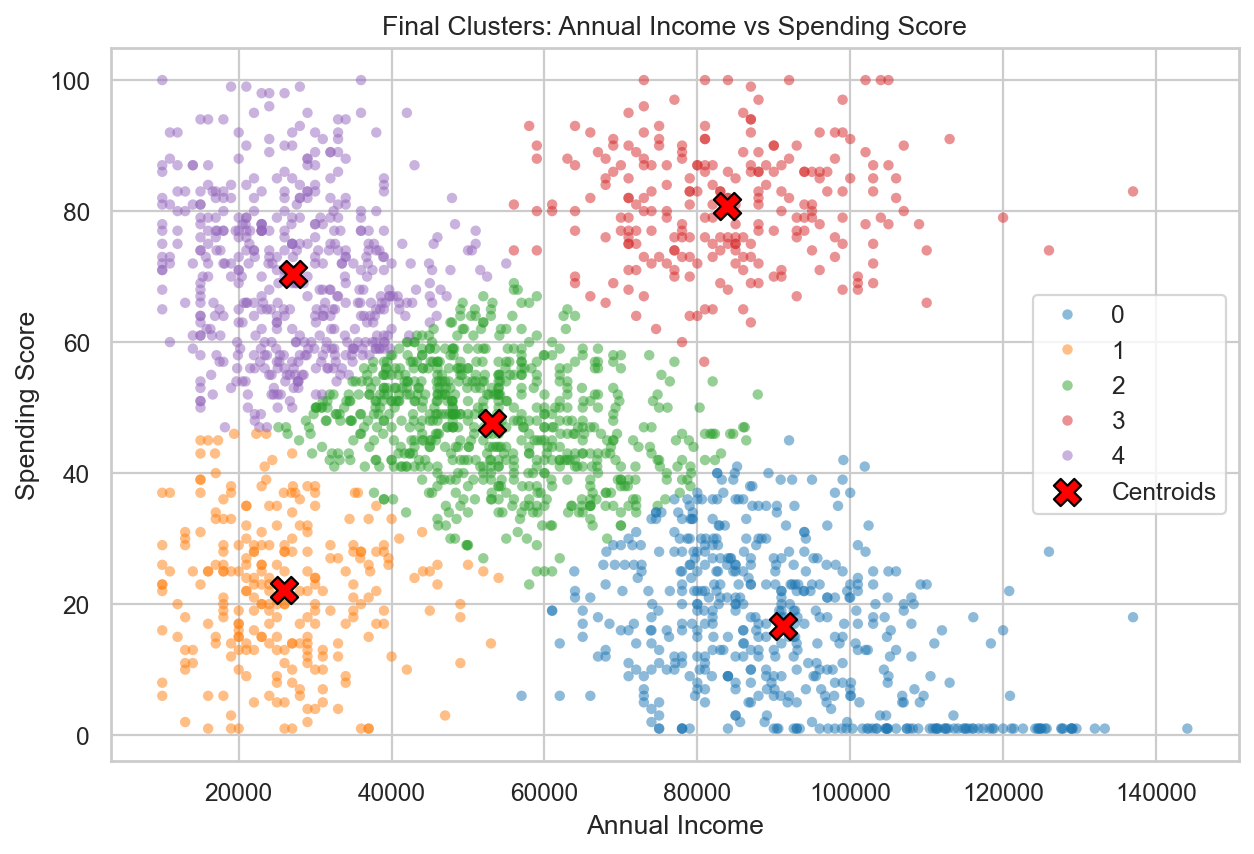
\includegraphics[width=0.85\textwidth]{figures/lab03/clusters_annual_income_vs_spending_score.png}
\caption{The most important clustering result: K=5 clusters on Income vs. Spending Score with centroid markers — 5 distinct, well-separated customer segments.}
\end{figure}

\subsubsection{Centroid Trajectory Visualization}
A dedicated sub-step replays the best K-Means run iteration-by-iteration, tracing centroid movement from random initialization to convergence. Well-behaved centroids move smoothly within 8–12 iterations without zigzagging or large jumps. Centroids that remain stationary from the start happened to land near the true center — rare but not a problem.

\begin{figure}[H]\centering
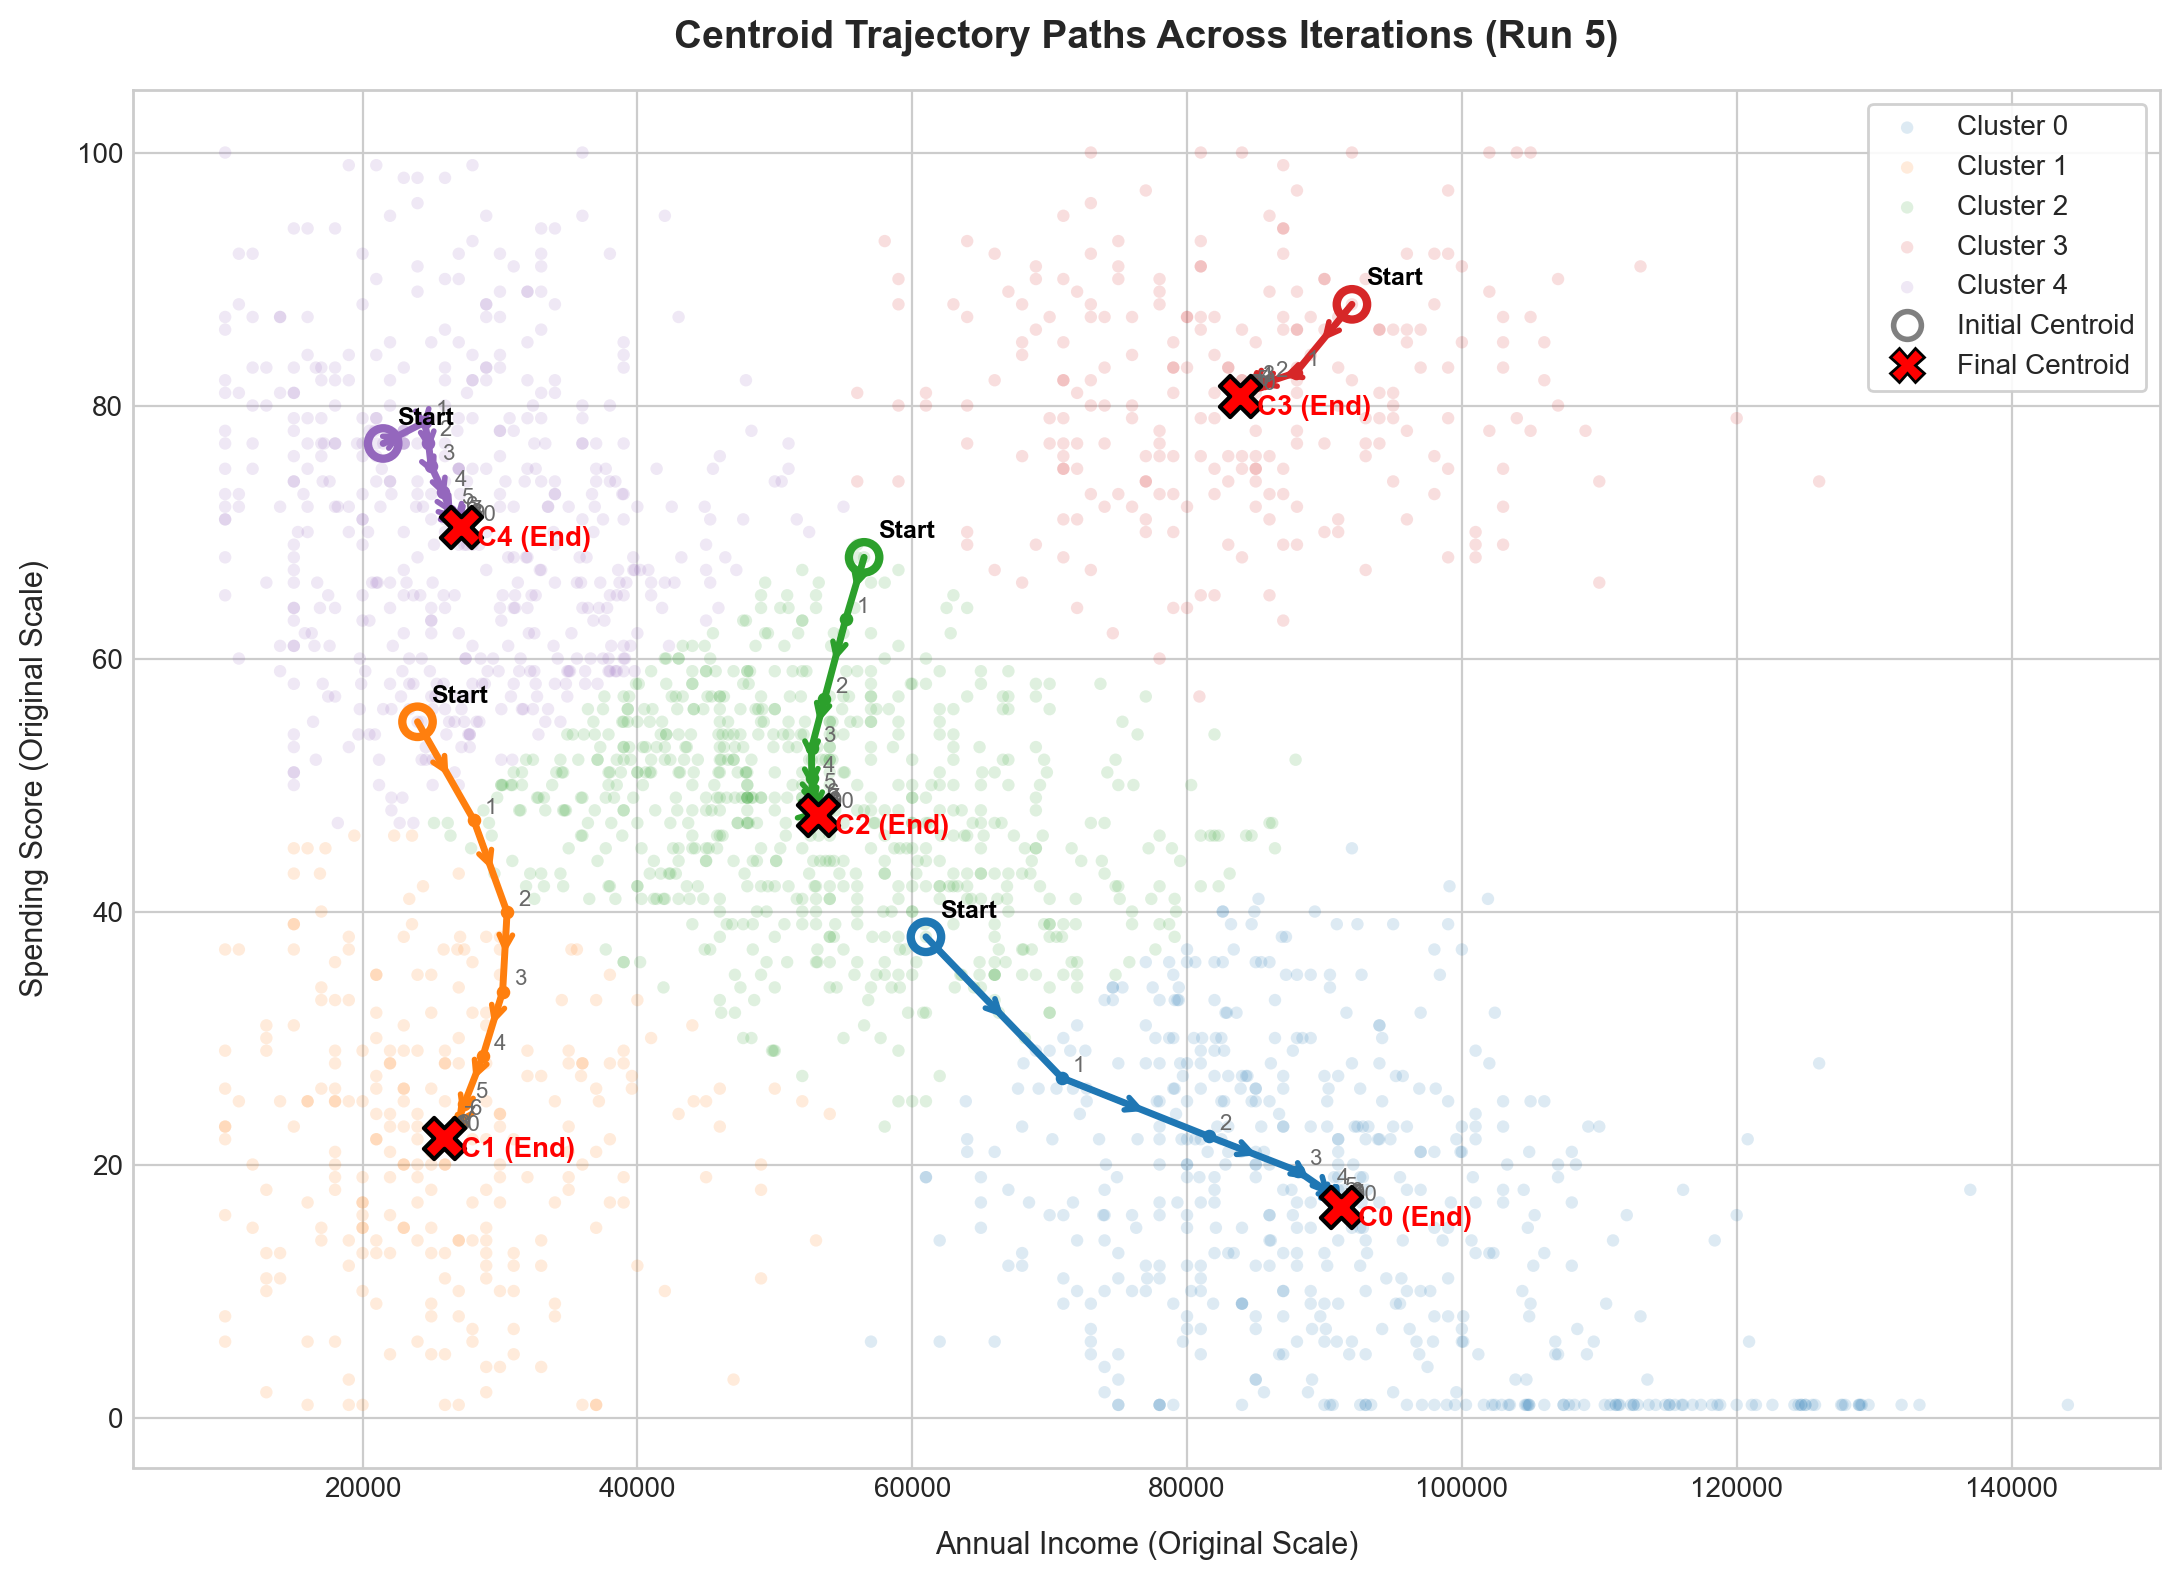
\includegraphics[width=0.78\textwidth]{figures/lab03/centroid_paths.png}
\caption{Centroid trajectory: iteration-by-iteration movement from k-means++ initialization to convergence. Smooth paths within 8–12 iterations confirm stable optimization.}
\end{figure}

\subsection{Step 8 — Cluster Visualization}

Four views confirm the model works \textit{visually}, not just statistically:
\begin{itemize}
  \item \textbf{Income vs. Spending scatter} — clusters must form distinct clouds; centroids near centroids of each cloud.
  \item \textbf{Age vs. Spending} — does age add a third discriminative dimension?
  \item \textbf{Age vs. Income} — complements the primary view.
  \item \textbf{PCA 2D projection} — first two principal components should show cluster separation.
\end{itemize}

Centroids are inverse-transformed to original scale (reversing StandardScaler) for business-interpretable coordinates. A GMM with 4 components and covariance ellipses ($1\sigma$, $2\sigma$, $3\sigma$) reveals cluster shape and orientation beyond K-Means's spherical assumption.

\begin{figure}[H]\centering
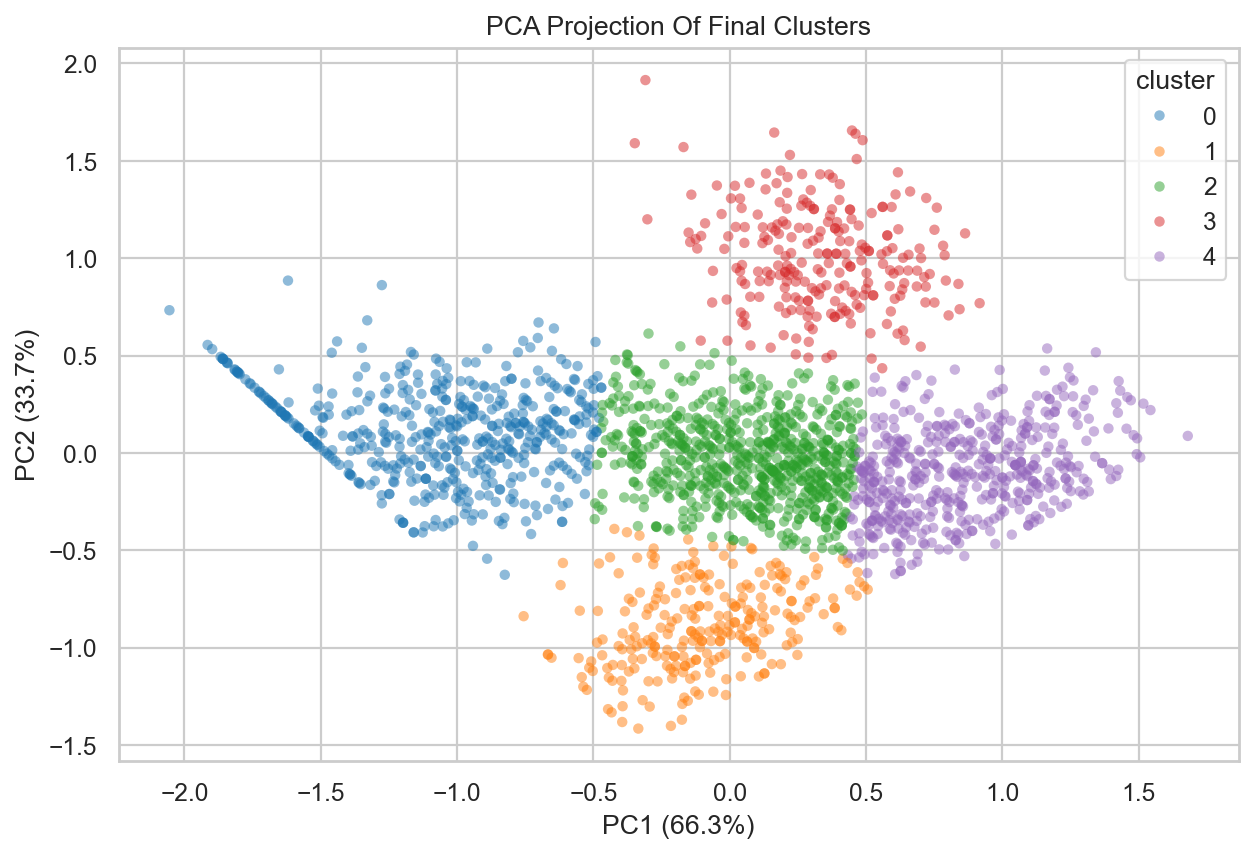
\includegraphics[width=0.78\textwidth]{figures/lab03/clusters_pca_projection.png}
\caption{PCA 2D projection: first two principal components with cluster assignments — confirms cluster separation in reduced dimensionality.}
\end{figure}

\begin{figure}[H]\centering
\begin{figure}[H]
  \centering
  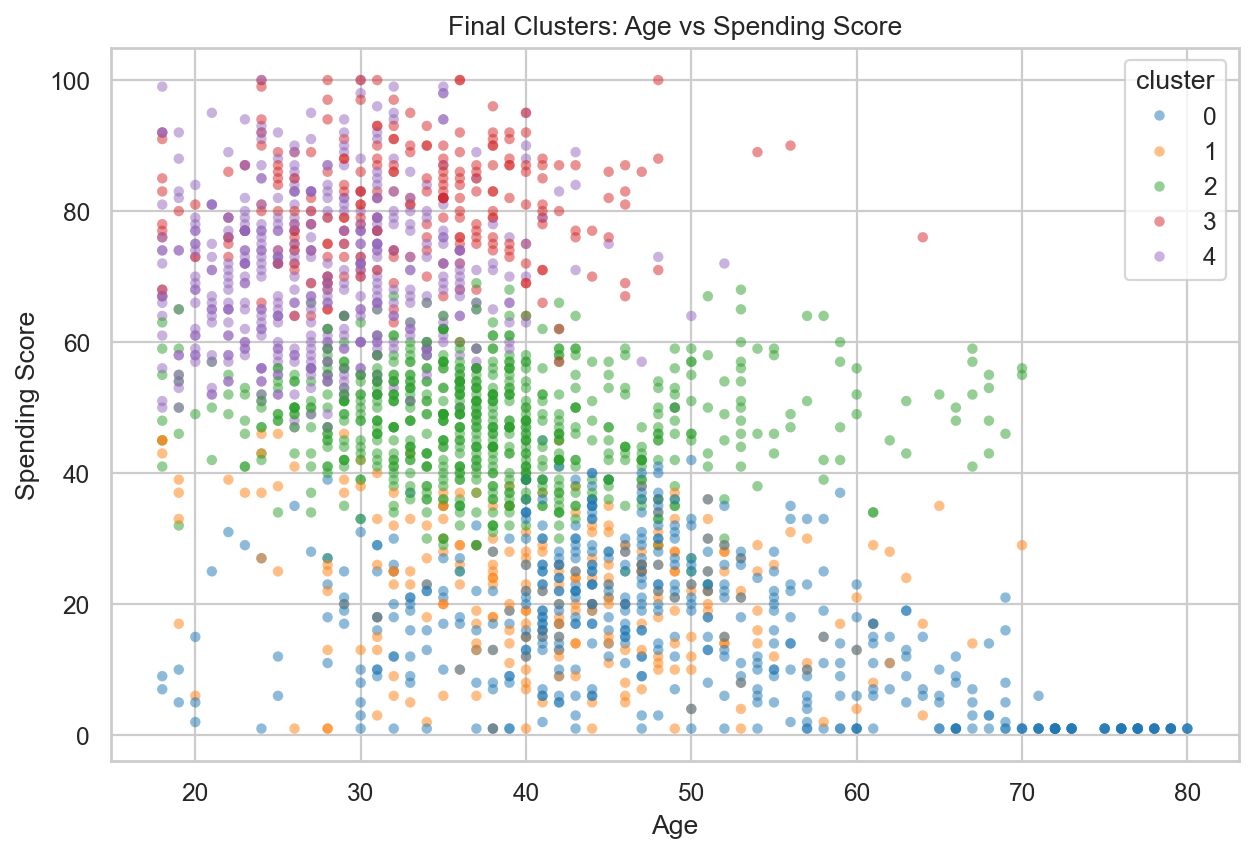
\includegraphics[width=\textwidth]{figures/lab03/clusters_age_vs_spending_score.png}
  \caption{Age vs. Spending Score}
\end{figure}
\begin{figure}[H]
  \centering
  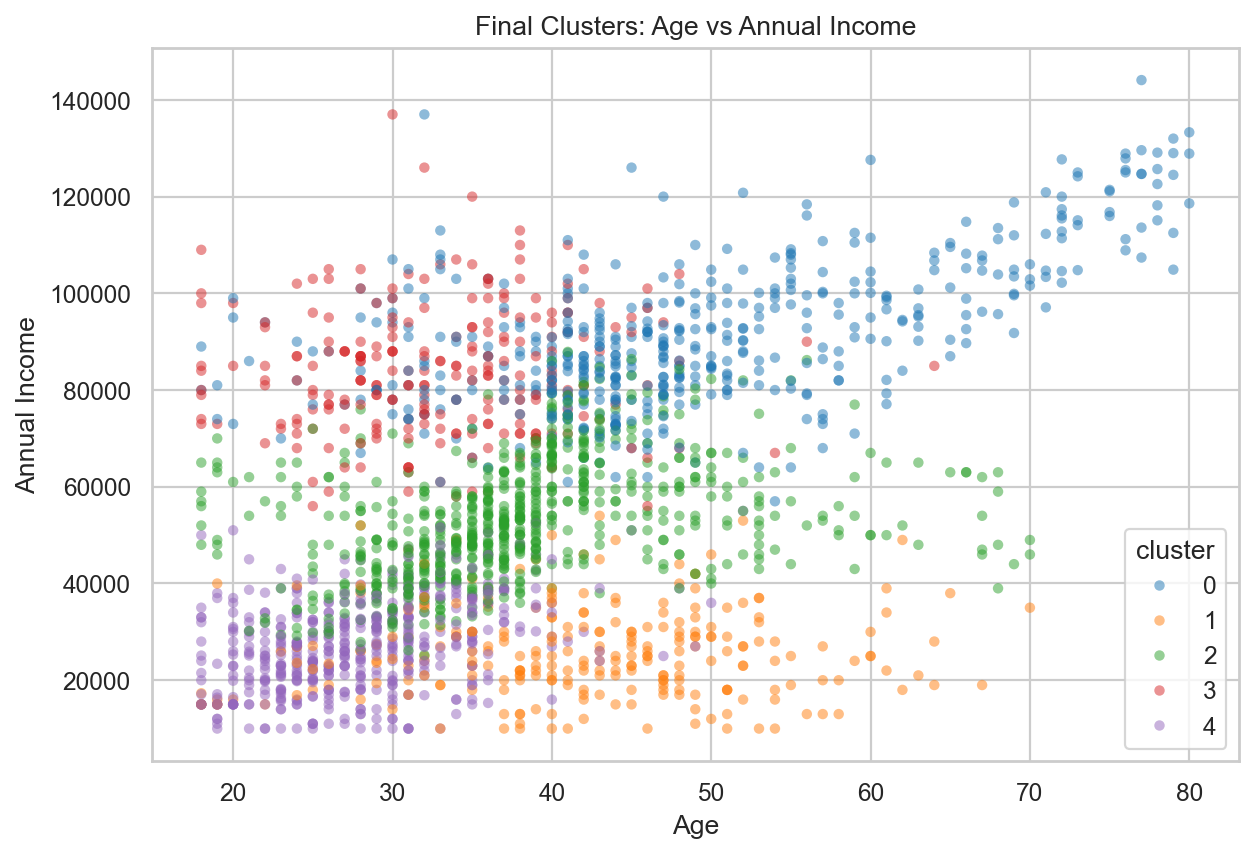
\includegraphics[width=\textwidth]{figures/lab03/clusters_age_vs_annual_income.png}
  \caption{Age vs. Annual Income}
\end{figure}
\end{figure}

\begin{figure}[H]\centering
\begin{figure}[H]
  \centering
  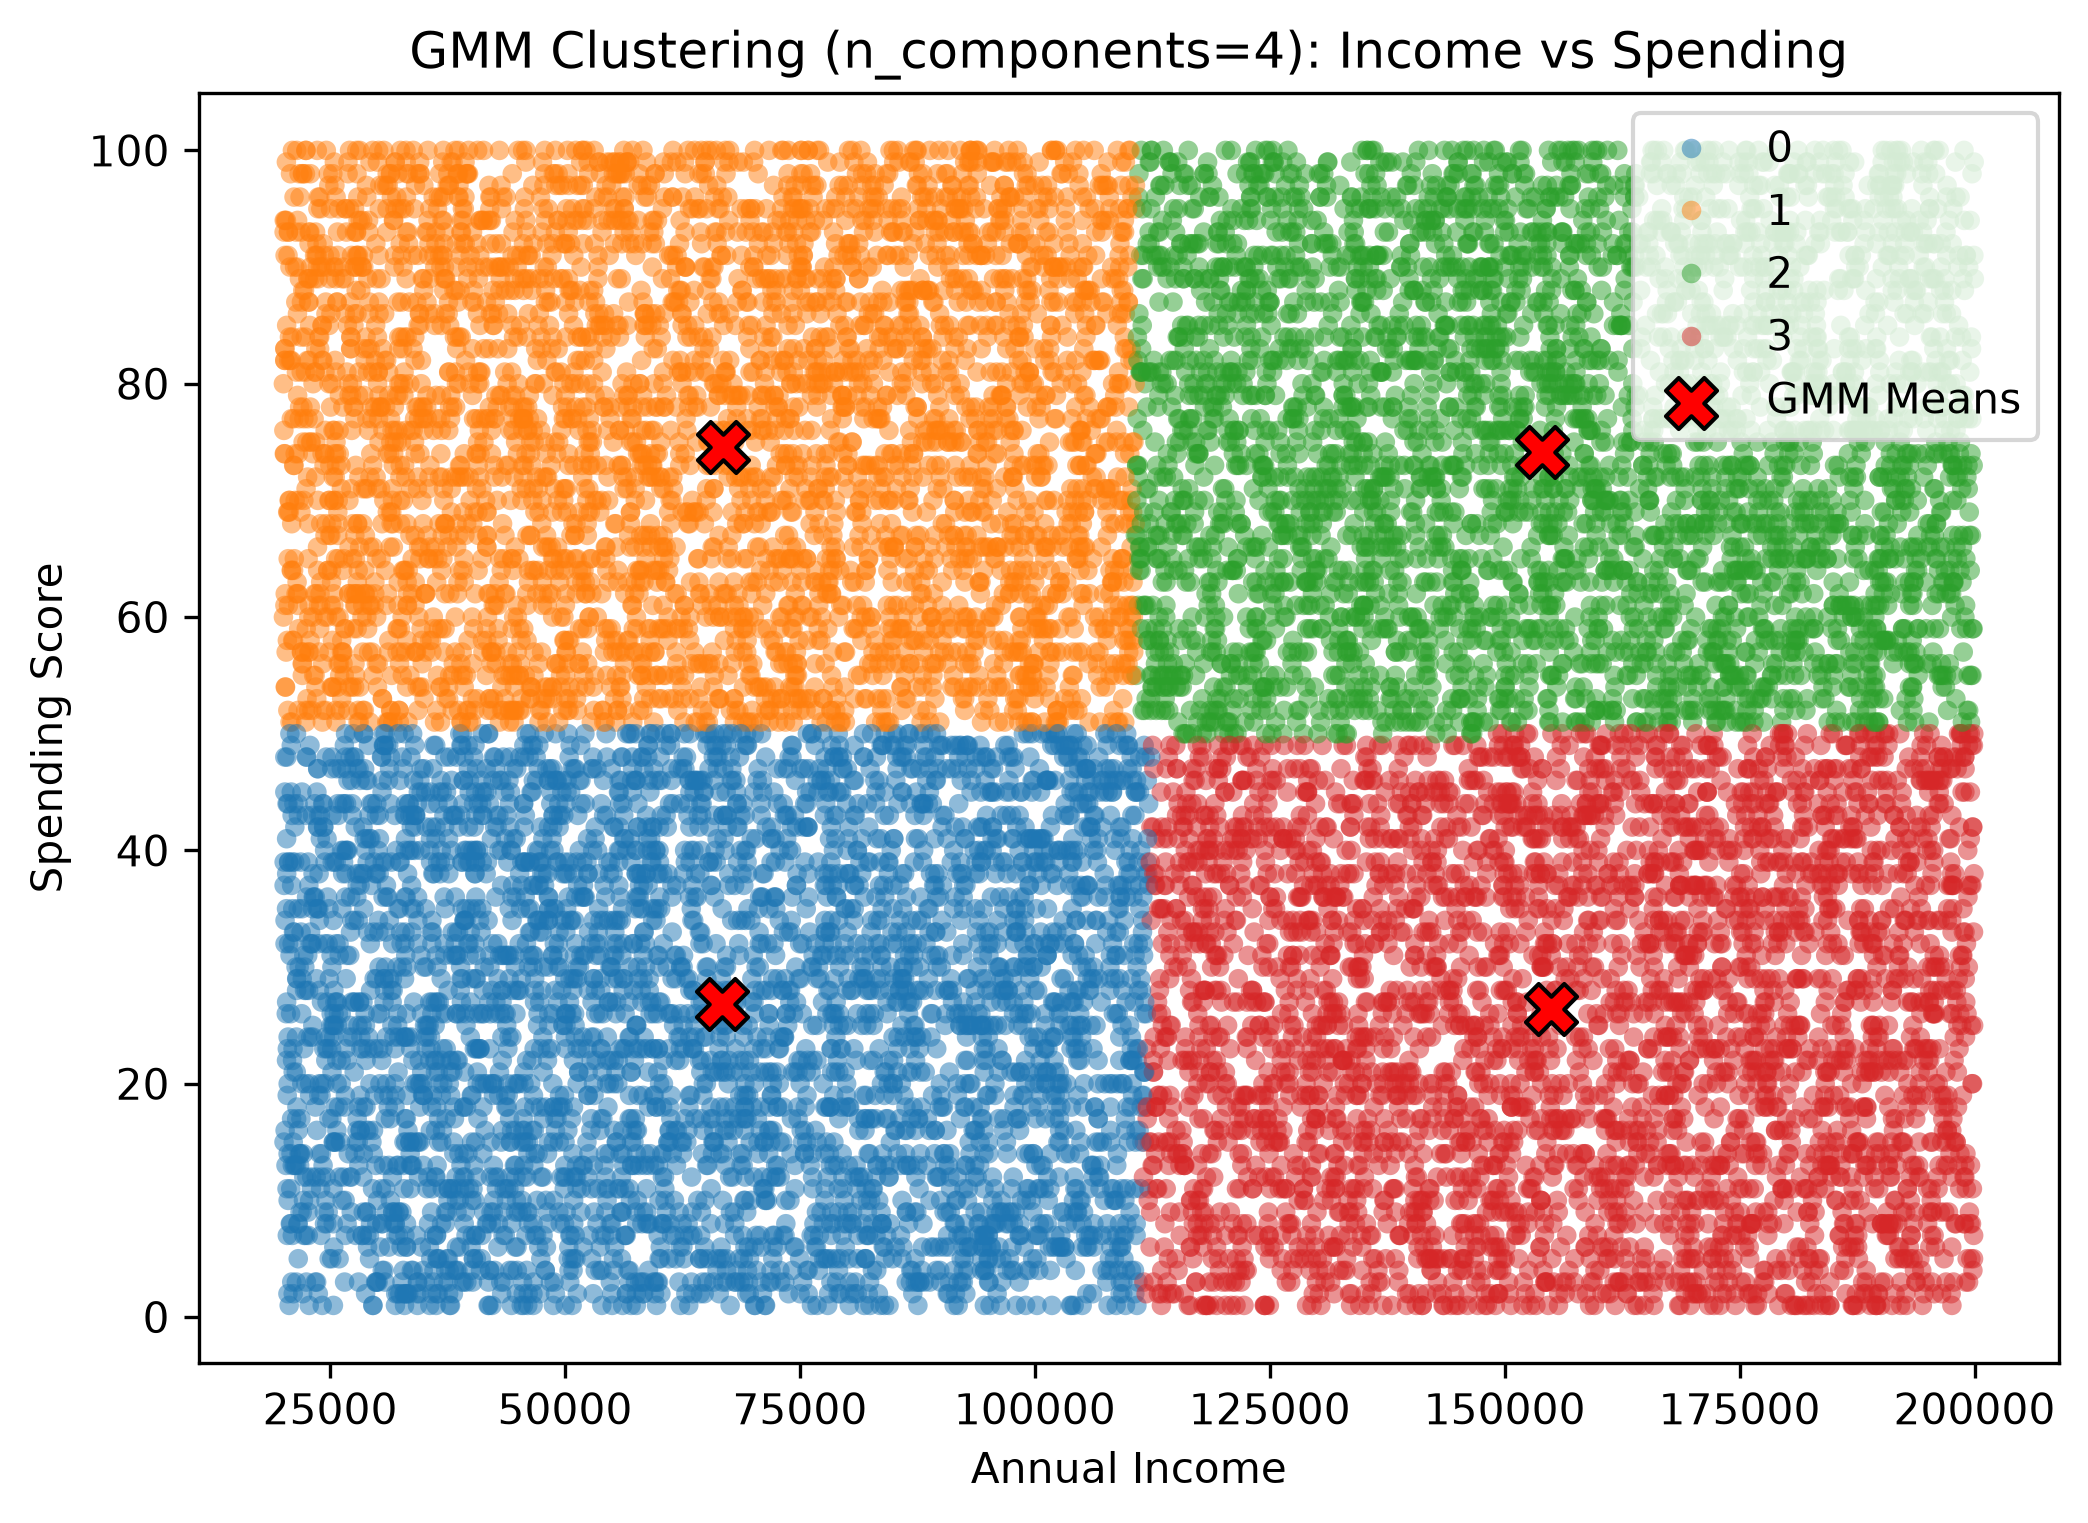
\includegraphics[width=\textwidth]{figures/lab03/gmm_income_vs_spending.png}
  \caption{GMM on Income vs. Spending}
\end{figure}
\begin{figure}[H]
  \centering
  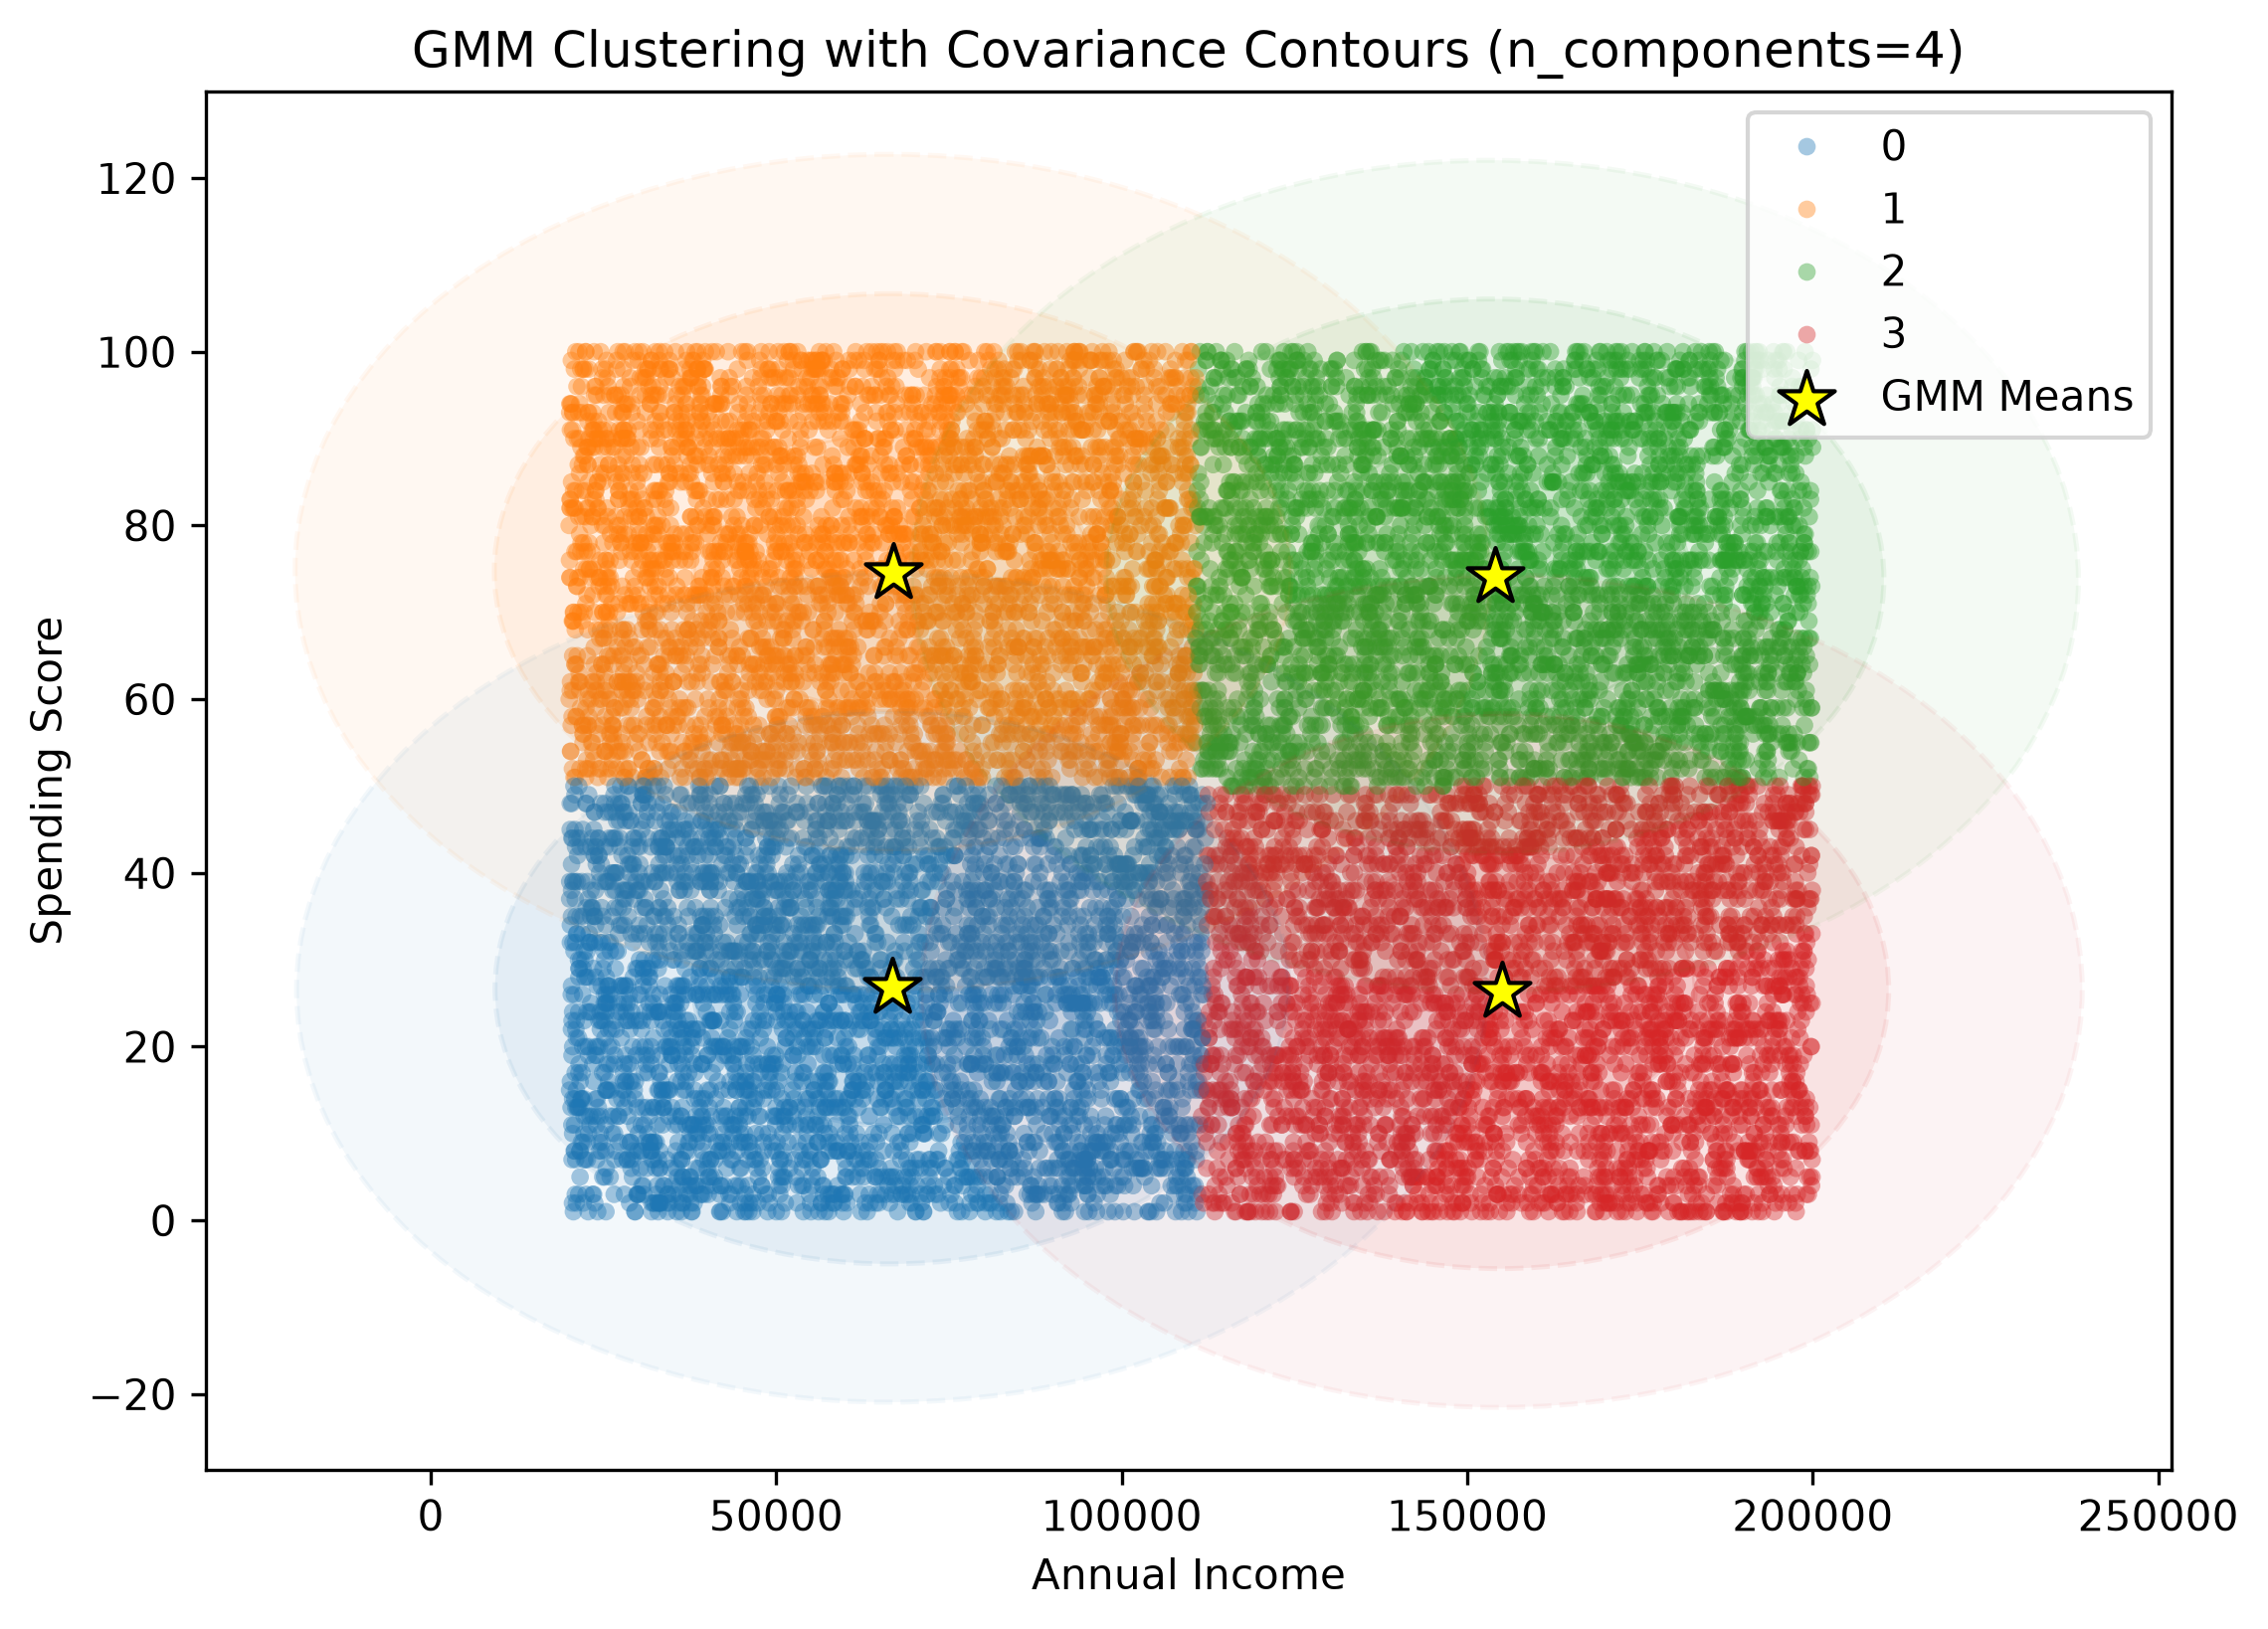
\includegraphics[width=\textwidth]{figures/lab03/gmm_contours.png}
  \caption{GMM covariance contours}
\end{figure}
\end{figure}

\subsection{Step 9 — Segment Profiling}

Each cluster's statistical fingerprint is translated into a human-readable name and concrete marketing action:

\begin{table}[H]
\centering\rowcolors{2}{tablerow}{white}
\begin{tabular}{c L{3.2cm} c c c L{3.5cm}}
\toprule\rowcolor{tablehead!80}\color{white}\textbf{Cl.} &\color{white}\textbf{Name} &\color{white}\textbf{Size} &\color{white}\textbf{Income} &\color{white}\textbf{Spending} &\color{white}\textbf{Strategy}\\
\midrule
0 & High Inc, Low Spend & 497 & \$91.2k & 16.6 & Incentives to convert\\
1 & Low Inc, Low Spend & 258 & \$26.0k & 22.1 & Low-cost engagement\\
2 & Moderate & 712 & \$53.2k & 47.7 & Retention \& seasonal offers\\
3 & High Inc, High Spend & 242 & \$83.9k & 80.7 & Loyalty \& premium perks\\
4 & Low Inc, High Spend & 491 & \$27.2k & 70.4 & Bundles \& value promos\\
\bottomrule
\end{tabular}
\caption{Five segments with recommended business actions}
\end{table}

\subsection{Step 11 — Deployment Check}
The fitted estimator, preprocessing transformer, feature names, and metadata are bundled into a single \texttt{joblib} file. A verification check loads the bundle and predicts a cluster for a dummy customer (35F, \$60K income, spending 50) to confirm end-to-end inference works independently of notebook state.

\section{Results and Analysis}

\begin{resultbox}
\textbf{Selected model:} K-Means, \textbf{K=5}, features = \texttt{income\_spending\_only}, \textbf{RobustScaler}.\\
\textbf{Silhouette: 0.4702} — well-separated clusters with strong structure.
\end{resultbox}

\begin{figure}[H]\centering
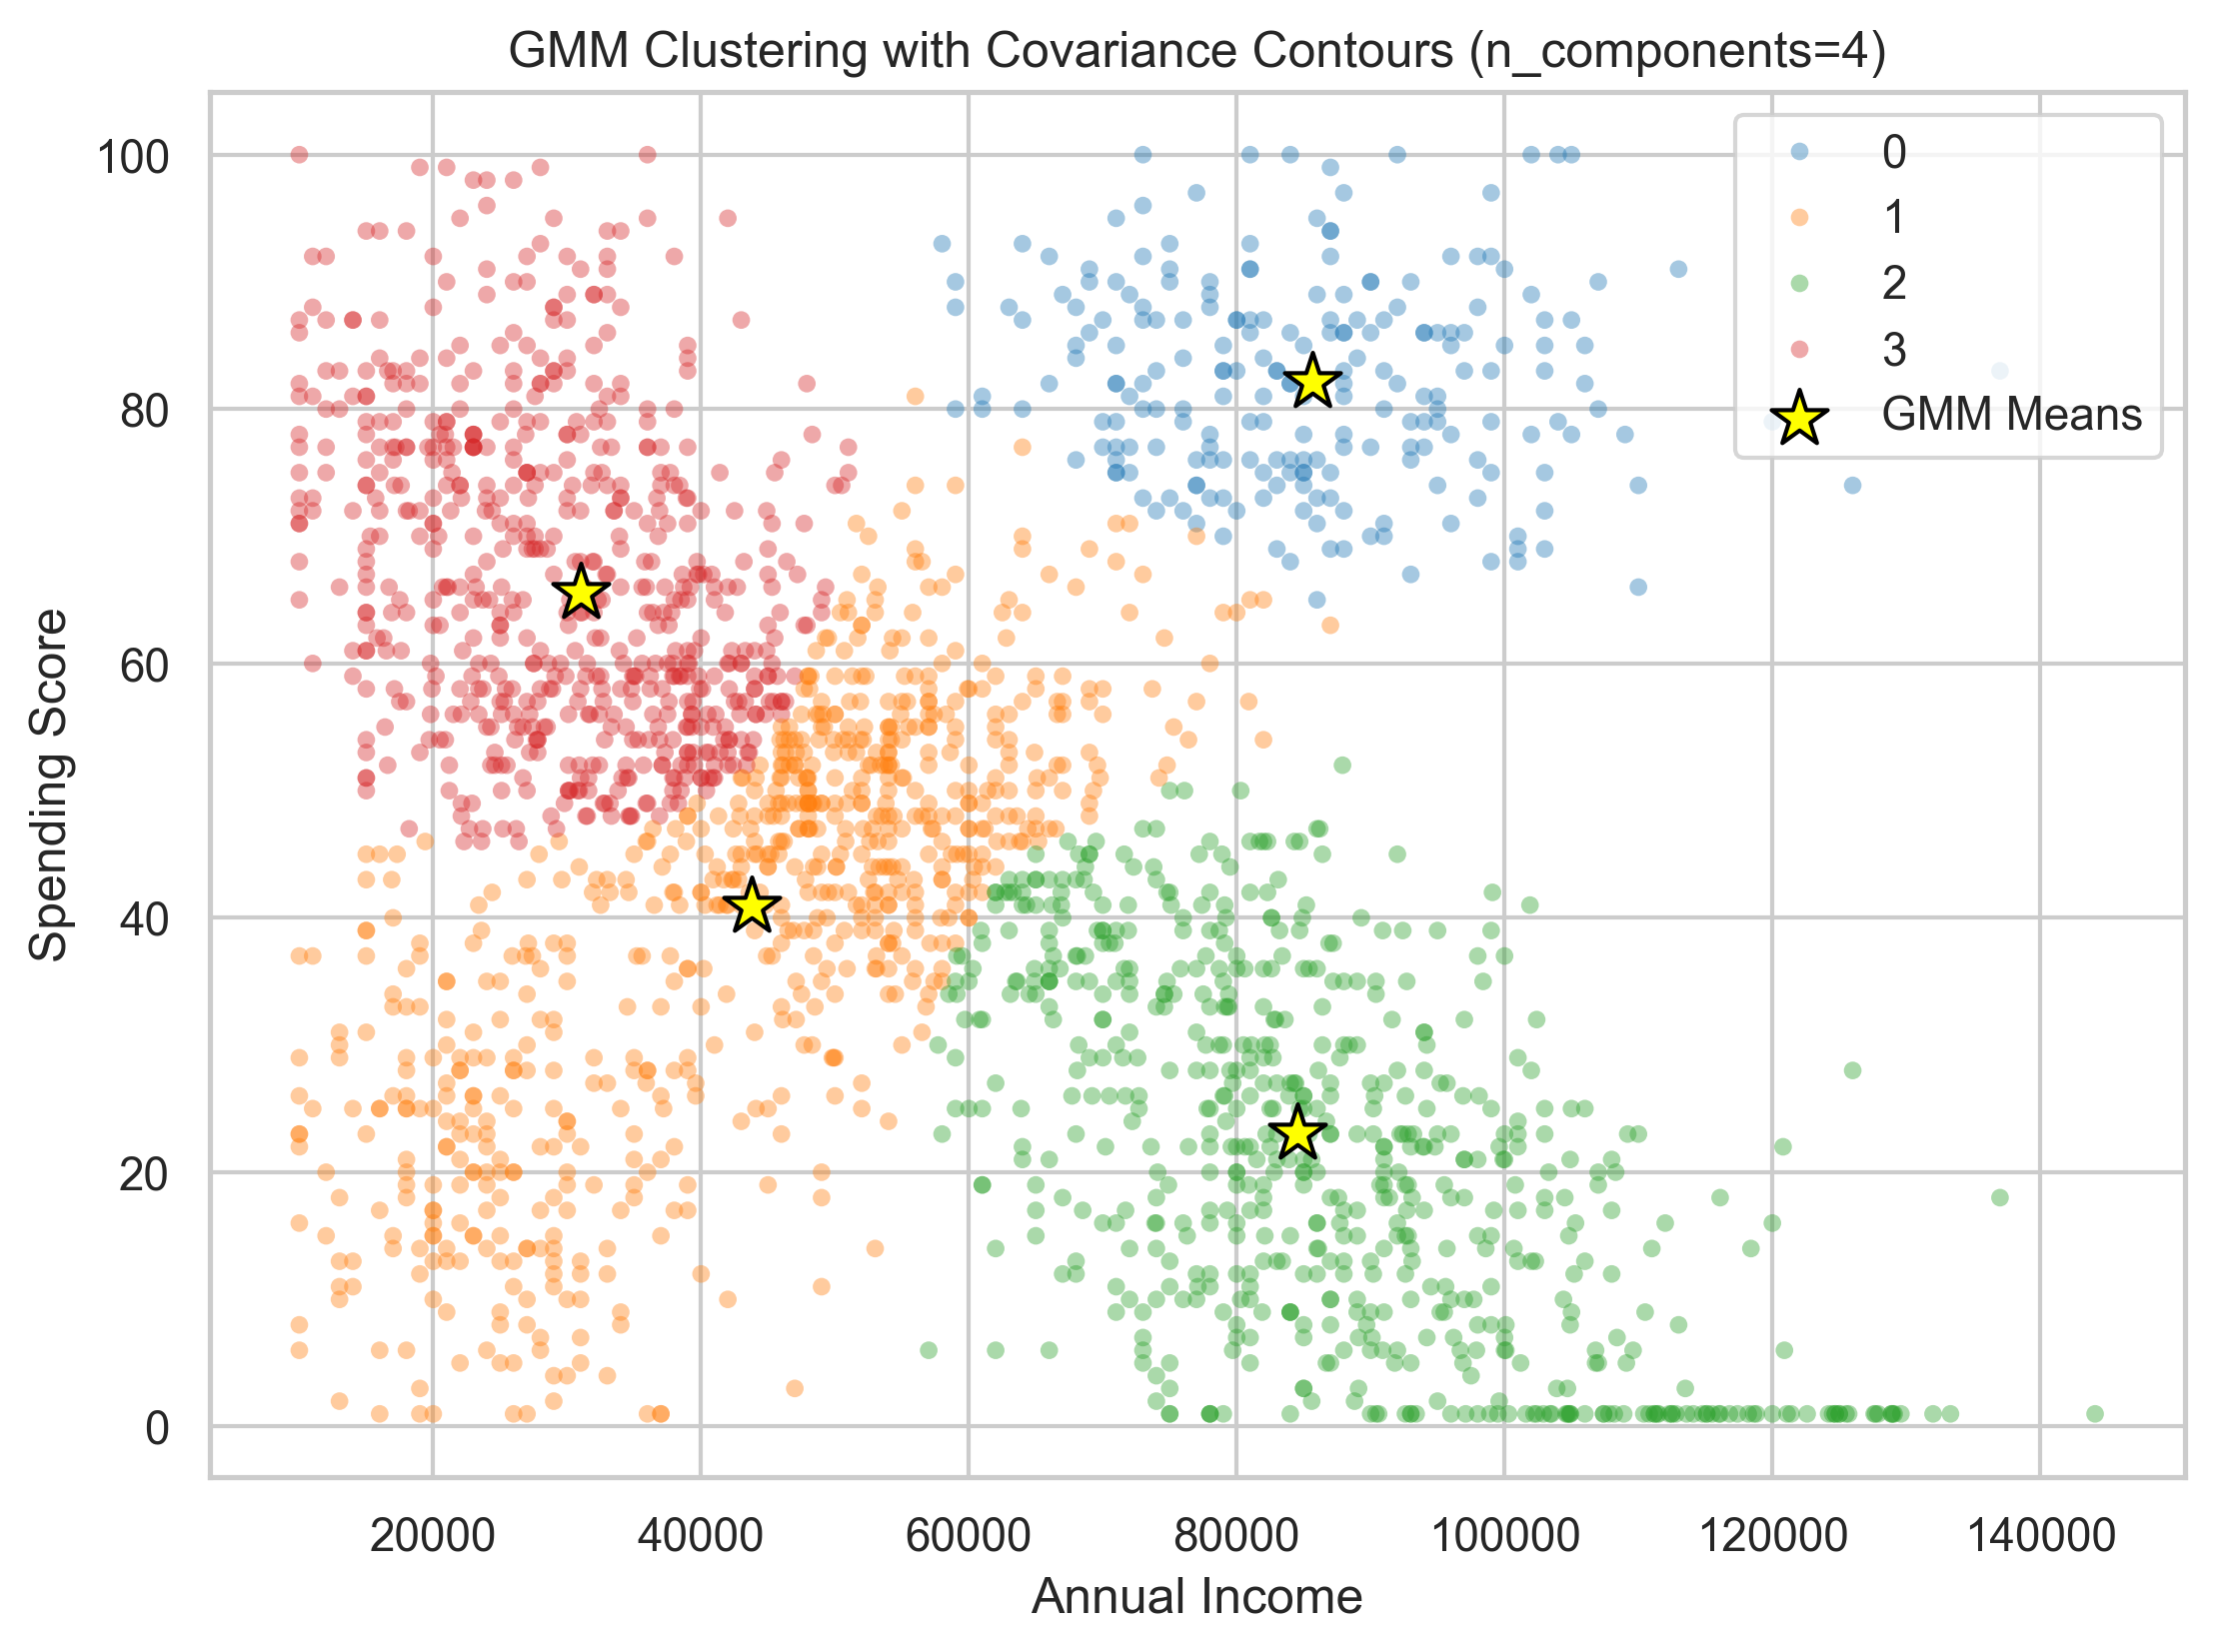
\includegraphics[width=0.7\textwidth]{figures/lab03/gmm_contours_comparison.png}
\caption{GMM with 4 components and covariance contours on Income vs. Spending scatter. Ellipses at 1$\sigma$, 2$\sigma$, and 3$\sigma$ reveal cluster shape and orientation.}
\end{figure}

\begin{figure}[H]\centering
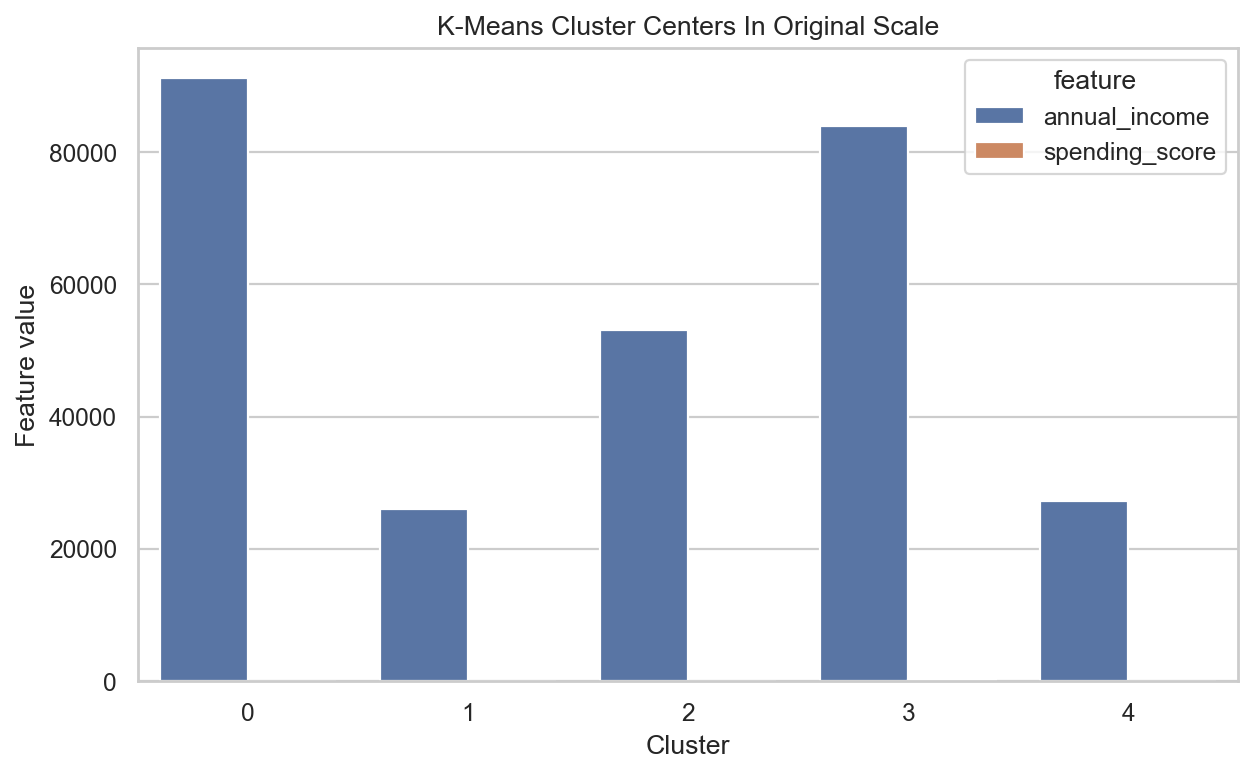
\includegraphics[width=0.78\textwidth]{figures/lab03/cluster_centers_original_scale.png}
\caption{Cluster centers in original feature scale — inverse-transformed from StandardScaler for business-interpretable segment profiles.}
\end{figure}

\begin{figure}[H]\centering
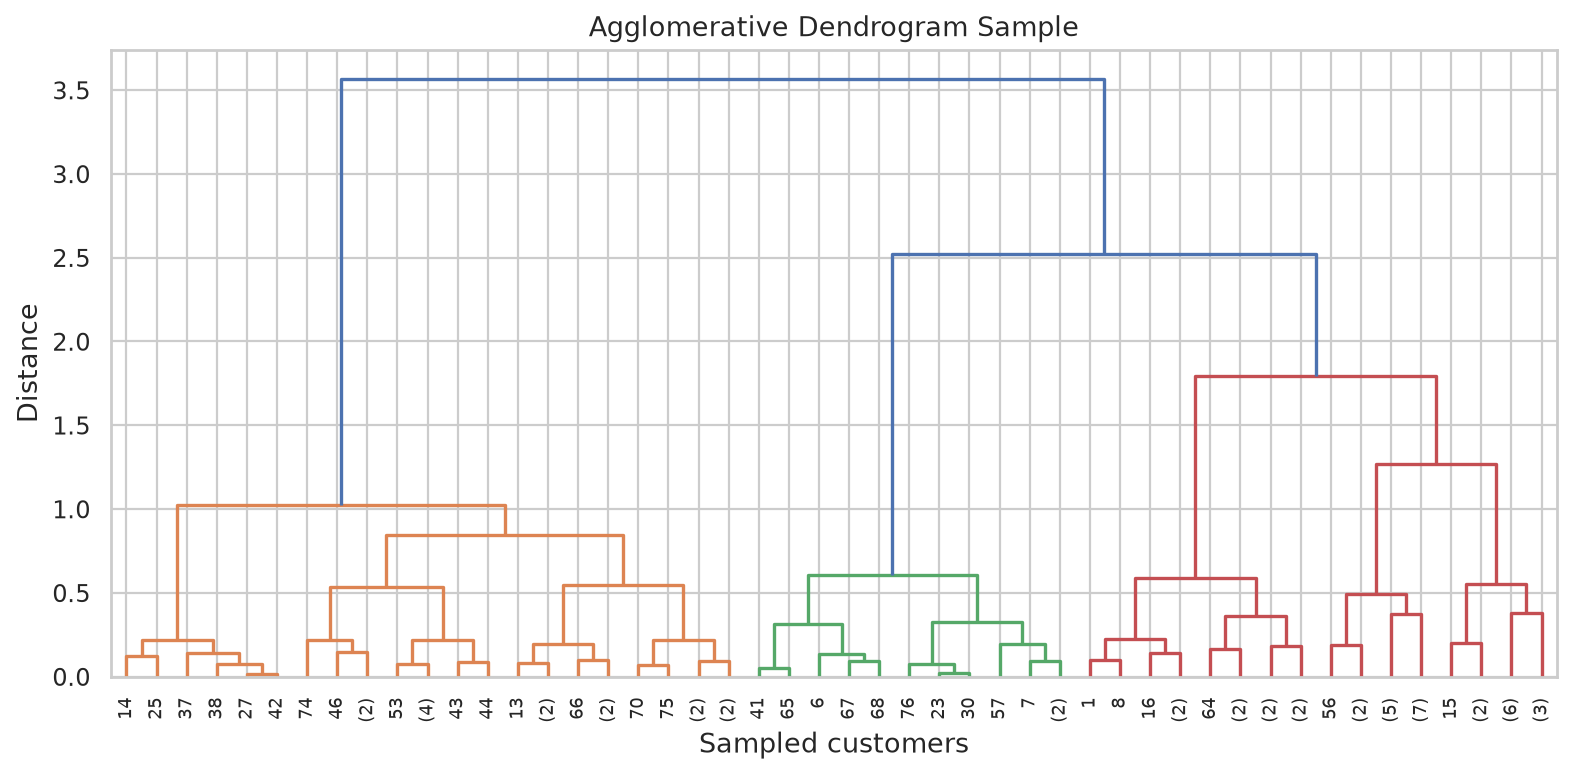
\includegraphics[width=0.78\textwidth]{figures/lab03/agglomerative_dendrogram_sample.png}
\caption{Agglomerative clustering dendrogram — hierarchical view of cluster merging distances on a sample subset.}
\end{figure}

\begin{notebox}
\textbf{Income/Spending naturally reveals 5 distinct groups.} Cluster 3 (high/high, 242 customers) is the most valuable segment — smallest but highest lifetime value. Cluster 1 (low/low, 258 customers) requires the lightest engagement: expensive campaigns waste budget here. Multi-criteria selection is critical — a single-metric sort would have overfit either inertia (picking K=10) or silhouette (ignoring cluster interpretability).
\end{notebox}

% ═══════════════════════════════════════════════════════════════
\chapter{Lab 3.1 — K-Means Image Segmentation}
\label{ch:lab31}
% ═══════════════════════════════════════════════════════════════

\section{Problem Definition}

\begin{problembox}
Apply K-Means clustering to \textbf{pixel color quantization}: reduce an RGB photograph from hundreds of thousands of unique colors to \textbf{K representative centroids}. The same algorithm underlying JPEG compression, artistic palette extraction, and automated object isolation. Evaluate K $\in \{2, 3, 5, 8\}$; select the K that best balances visual fidelity and compression.
\end{problembox}

\subsection{Dataset}
\begin{itemize}
  \item \textbf{Input:} Three RGB photographs — primary image resized to $262\times350 = 91{,}700$ pixels. If absent, a deterministic landscape is synthesized.
  \item \textbf{Feature space:} Each pixel is a point in $\mathbb{R}^3$ with (R, G, B) channels $\in [0, 255]$.
\end{itemize}

\section{Complete Workflow}

\subsection{Step 0 — Setup and Reproducibility}
The random seed (42) guarantees identical centroid initialization across runs. Five custom modules — \texttt{utils}, \texttt{image\_io}, \texttt{kmeans}, \texttt{visualization}, \texttt{run\_pipeline} — are imported from \texttt{src/}. Output directories are created: \texttt{data/raw/} (source images), \texttt{data/processed/} (resized and segmented artifacts), \texttt{reports/figures/} (all plots).

\subsection{Step 1 — Load the Image}
Three image filenames are iterated. For each image, a summary prints: shape, dtype, pixel intensity range, and \textbf{unique RGB color count} — the baseline for measuring compression ratio. A healthy 350px image yields 3,000–30,000 unique colors. The displayed image confirms the file loaded correctly.

\begin{figure}[H]\centering
\begin{figure}[H]
  \centering
  \includegraphics[width=\textwidth]{figures/lab31/original_picture.png}
  \caption{Original Picture 1}
\end{figure}
\begin{figure}[H]
  \centering
  \includegraphics[width=\textwidth]{figures/lab31/original_picture_2.png}
  \caption{Original Picture 2}
\end{figure}
\begin{figure}[H]
  \centering
  
\includegraphics[width=\textwidth]{figures/lab31/original_picture_3.png}
  \caption{Original Picture 3}
\end{figure}
\end{figure}

\begin{figure}[H]\centering
\includegraphics[width=0.7\textwidth]{figures/lab31/original_image.png}
\caption{Primary image loaded for K-Means pixel clustering.}
\end{figure}

\subsection{Step 2 — Preprocess the Image}
\begin{enumerate}
  \item \textbf{Resize:} Max dimension capped at 350px — an uncompressed 4000$\times$3000 image (12M points) is computationally prohibitive. 350px bounds pixels to $\sim$122,500, large enough to preserve spatial structure but fast enough for clustering in seconds.
  \item \textbf{Flatten:} \texttt{flatten\_pixels()} reshapes $(H, W, C) \rightarrow (H\!\times\!W, C)$ — the canonical input for vectorized distance computations.
  \item \textbf{Color space preview:} The image is rendered in RGB, HSV, and LAB for visual comparison. \textbf{RGB} clusters raw channel co-occurrence; \textbf{HSV} separates chromatic content (hue) from intensity (value); \textbf{LAB} approximates human perceptual distance — Euclidean proximity in LAB correlates more closely with visible color difference.
\end{enumerate}

\begin{figure}[H]\centering
\begin{figure}[H]
  \centering
  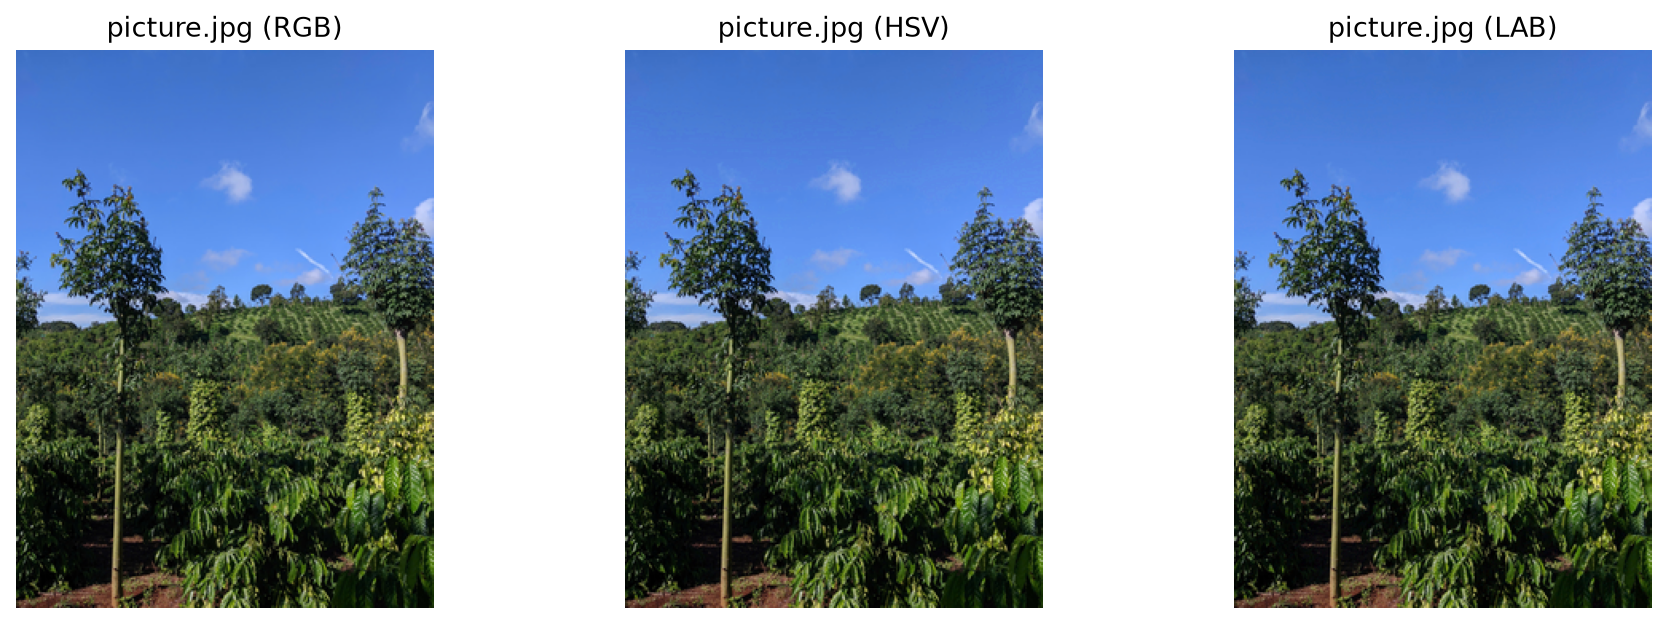
\includegraphics[width=\textwidth]{figures/lab31/color_space_preview_picture.png}
  \caption{Color spaces: Picture 1}
\end{figure}
\begin{figure}[H]
  \centering
  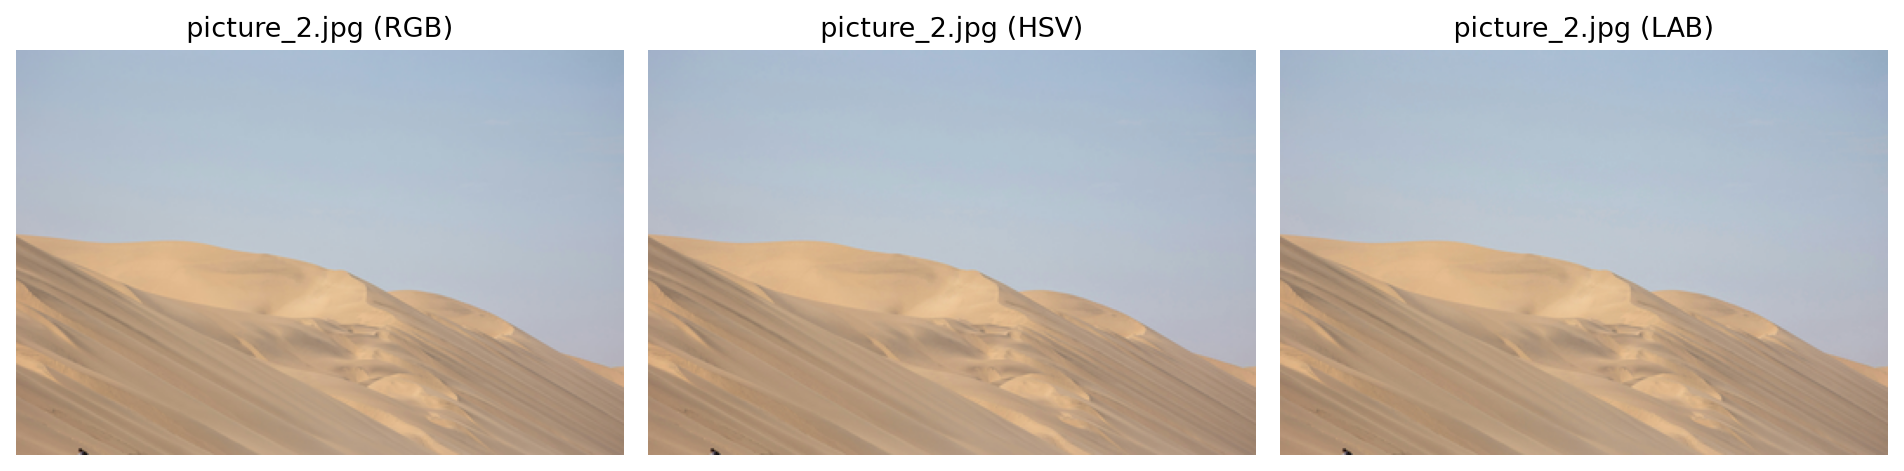
\includegraphics[width=\textwidth]{figures/lab31/color_space_preview_picture_2.png}
  \caption{Color spaces: Picture 2}
\end{figure}
\begin{figure}[H]
  \centering
  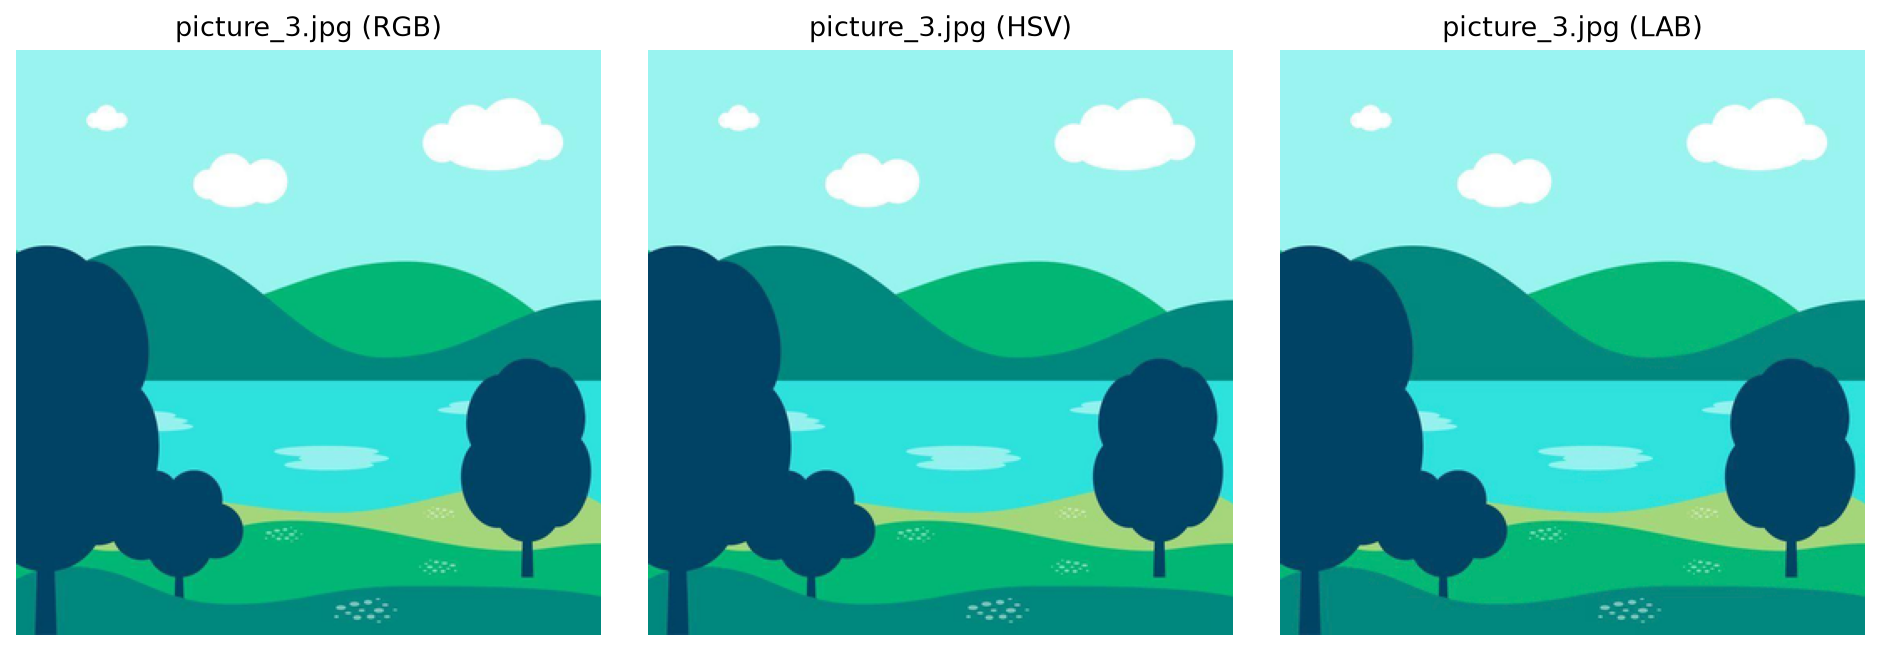
\includegraphics[width=\textwidth]{figures/lab31/color_space_preview_picture_3.png}
  \caption{Color spaces: Picture 3}
\end{figure}
\end{figure}

\begin{figure}[H]\centering
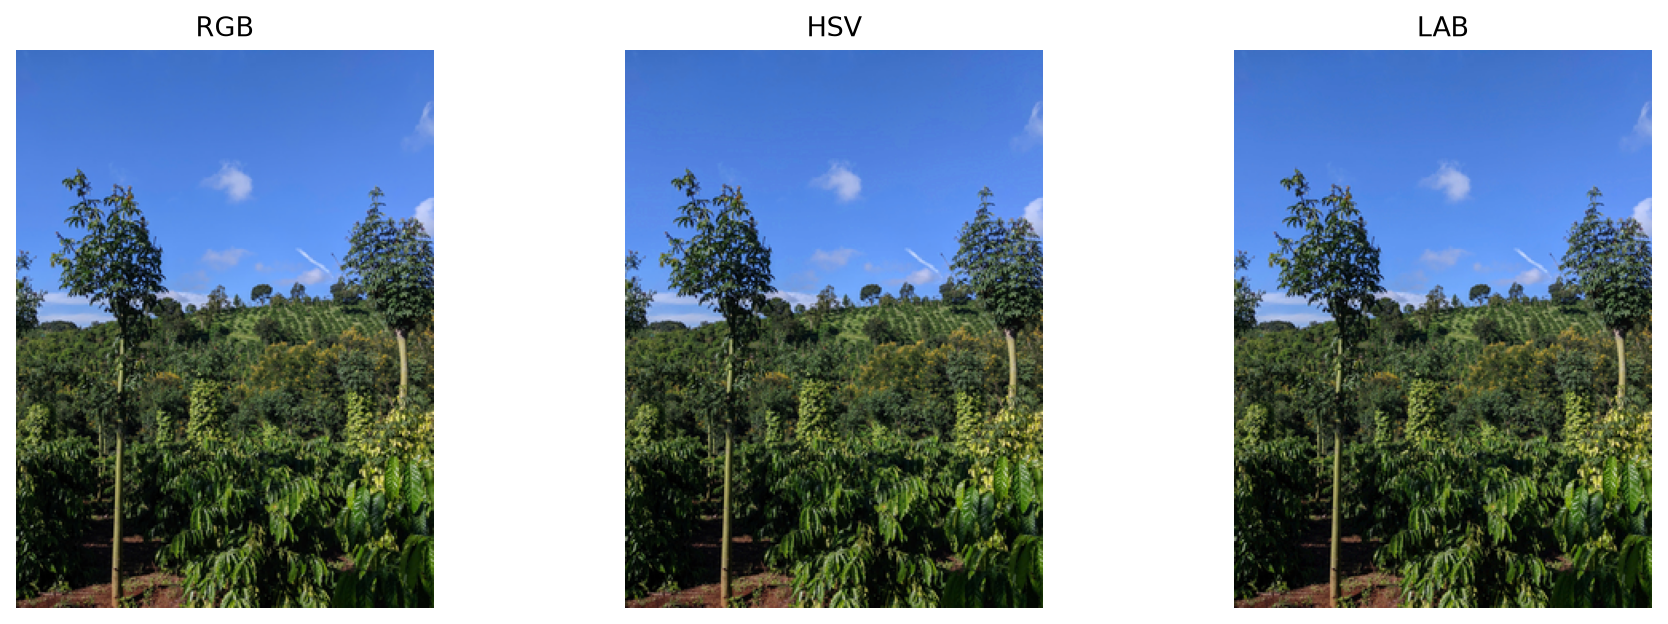
\includegraphics[width=0.78\textwidth]{figures/lab31/color_space_preview.png}
\caption{Primary image color space comparison: RGB vs. HSV vs. LAB rendering. LAB provides perceptually uniform distances.}
\end{figure}

\subsection{Step 3 — Inspect the K-Means Implementation}
\texttt{KMeansFromScratch} is instantiated with K=3 and printed. The implementation uses zero scikit-learn calls — every operation is NumPy:
\begin{itemize}
  \item \textbf{Initialization:} Selects K random pixels as starting centroids.
  \item \textbf{Assignment:} Squared Euclidean distance from every pixel to every centroid; assign to nearest.
  \item \textbf{Update:} Recompute centroids as the channel-wise mean of all assigned pixels.
  \item \textbf{Convergence:} Terminate when mean centroid displacement $<$ \texttt{tol}. Empty clusters are re-seeded from the farthest point.
\end{itemize}

Centroid shift is tracked as the \textbf{mean} Euclidean displacement — more stable than maximum displacement when one cluster converges slowly while others have settled.

\subsection{Step 4 — K-Means Grid Experiment}
The core experiment: for each image and K, fit the custom model, reconstruct the segmented image, and collect metrics:

\begin{table}[H]
\centering\rowcolors{2}{tablerow}{white}
\begin{tabular}{c c c c}
\toprule\rowcolor{tablehead!80}\color{white}\textbf{K} &\color{white}\textbf{Visual Result} &\color{white}\textbf{Use Case} &\color{white}\textbf{Expected Iters}\\
\midrule
2 & Harsh two-tone posterization & Silhouette extraction, binary masks & 5–10\\
3 & Sky/ground/object separation & Simple landscape segmentation & 10–20\\
5 & Texture preserved, edges sharp & Balanced compression & 20–30\\
8 & Near-photographic fidelity & Near-lossless color reduction & 30–50\\
\bottomrule
\end{tabular}
\caption{Expected behavior per K value}
\end{table}

\subsubsection{Metrics Collected Per Run}
\begin{itemize}
  \item \textbf{Inertia:} Within-cluster sum of squared distances. Always decreases with K — never use alone.
  \item \textbf{Iterations to convergence:} If $\text{n\_iter\_} = \text{max\_iter}$, the model did not converge.
  \item \textbf{Silhouette:} Computed on a 2,000-pixel random sample (full $O(N^2)$ pairwise distance on 91k pixels would require $>50$ GB RAM). Values $>0.5$ = strong structure; $<0.2$ = overlapping clusters.
  \item \textbf{Compression ratio:} $\text{unique\_colors\_before} / \text{unique\_colors\_after}$. A ratio of 1000:1 means thousands of colors compressed to K.
\end{itemize}

\subsection{Step 4.1 — Elbow Method}
Inertia is plotted against K. The ``elbow'' — where marginal gain flattens — identifies diminishing returns. For landscape images, the bend is at K=3–5. When no obvious bend exists (smooth gradient images), silhouette analysis serves as the tie-breaker.

\subsection{Step 4.2 — Silhouette Analysis}
Per-pixel silhouette: $s(i) = (b(i) - a(i)) / \max(a(i), b(i))$, where $a(i)$ is mean intra-cluster distance and $b(i)$ is mean distance to the nearest other cluster. The red dashed line marks the average. Uniformly thick bars at high scores indicate compact, well-separated clusters; thin bars near zero signal overlap.

\begin{figure}[H]\centering
\begin{figure}[H]
  \centering
  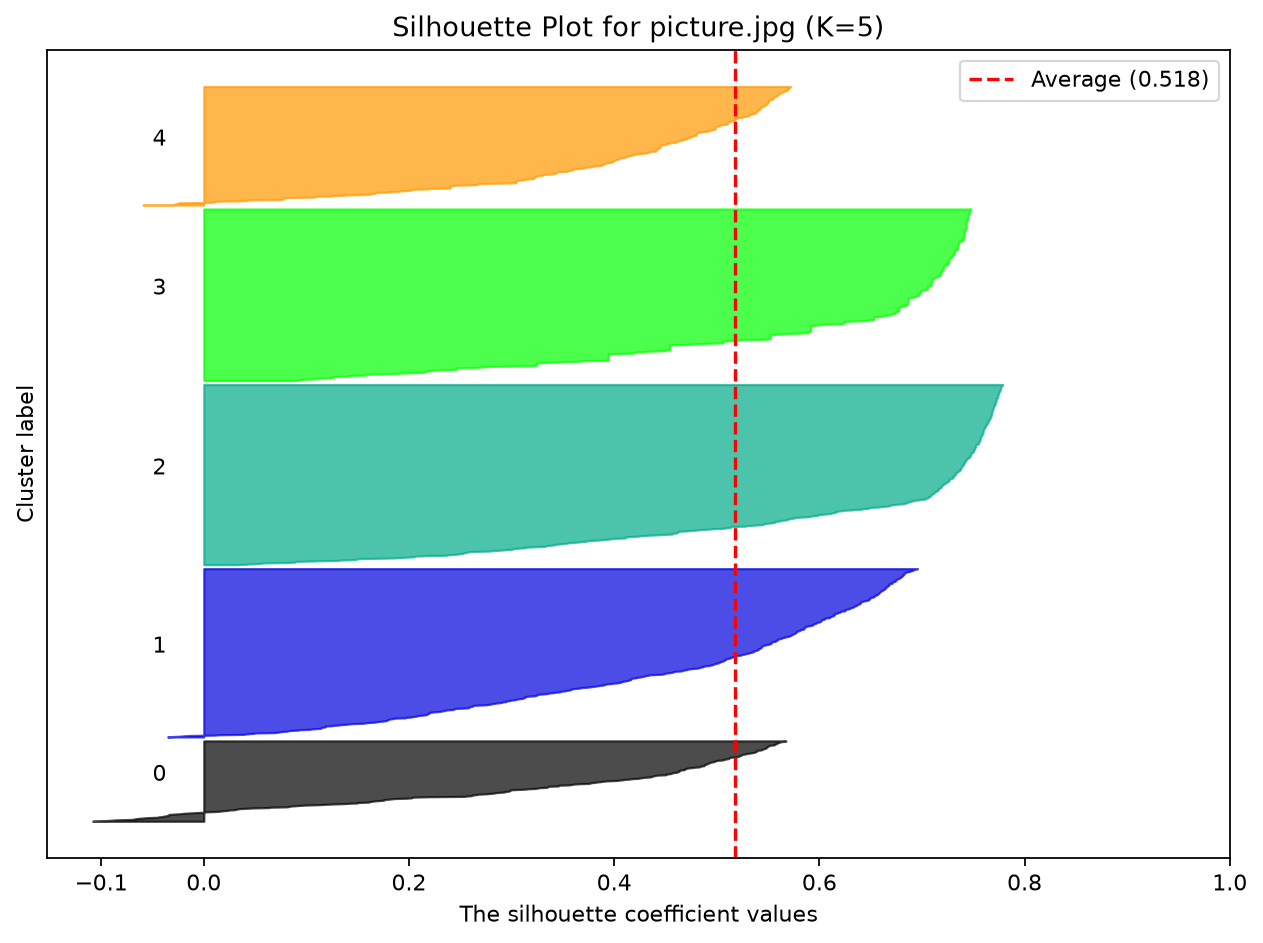
\includegraphics[width=\textwidth]{figures/lab31/silhouette_plot_picture_k5.png}
  \caption{Silhouette: Picture 1 at K=5}
\end{figure}
\begin{figure}[H]
  \centering
  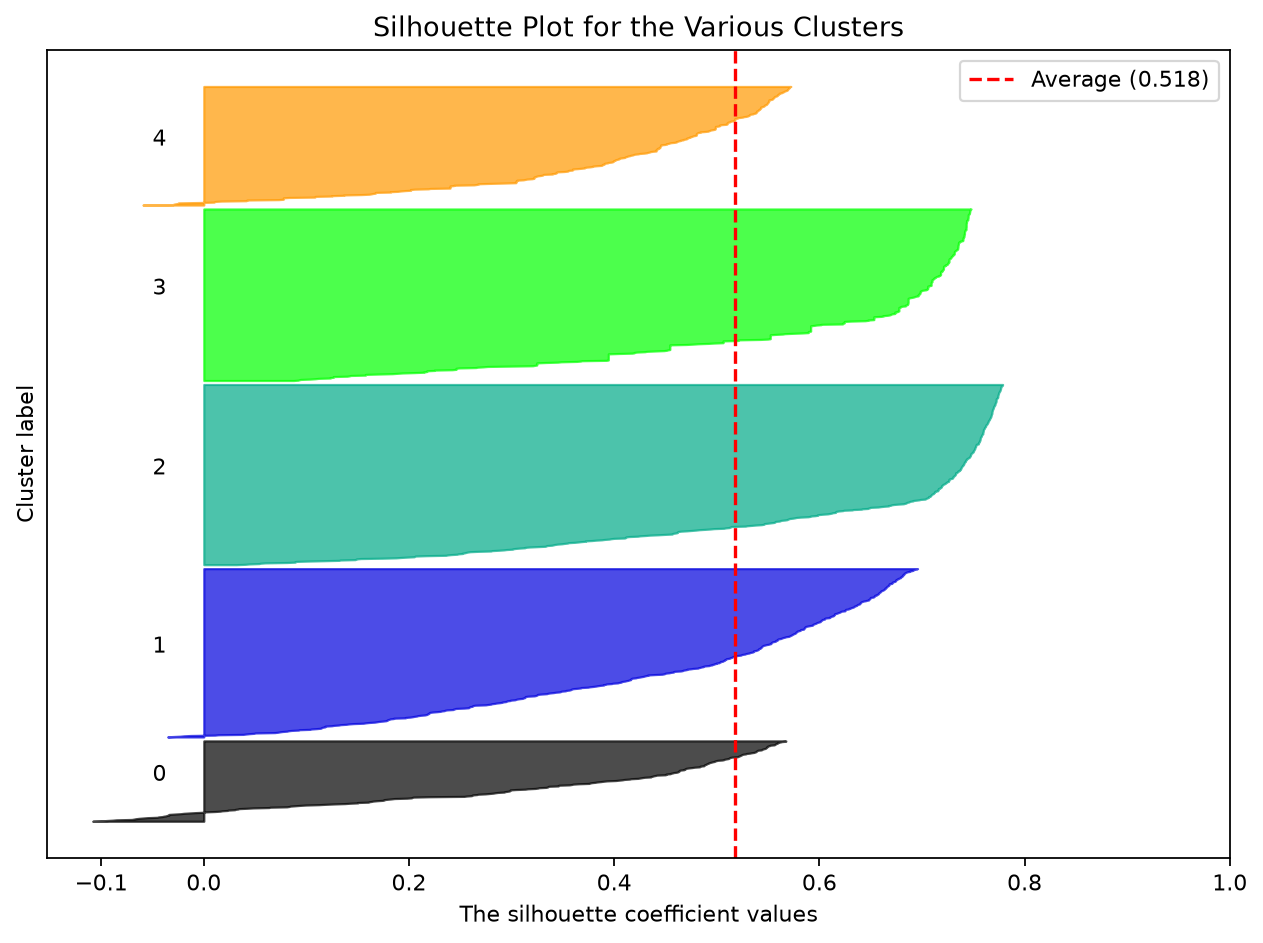
\includegraphics[width=\textwidth]{figures/lab31/silhouette_plot_k5.png}
  \caption{Silhouette: K=5 detail}
\end{figure}\
\vspace{4pt}
\begin{figure}[H]
  \centering
  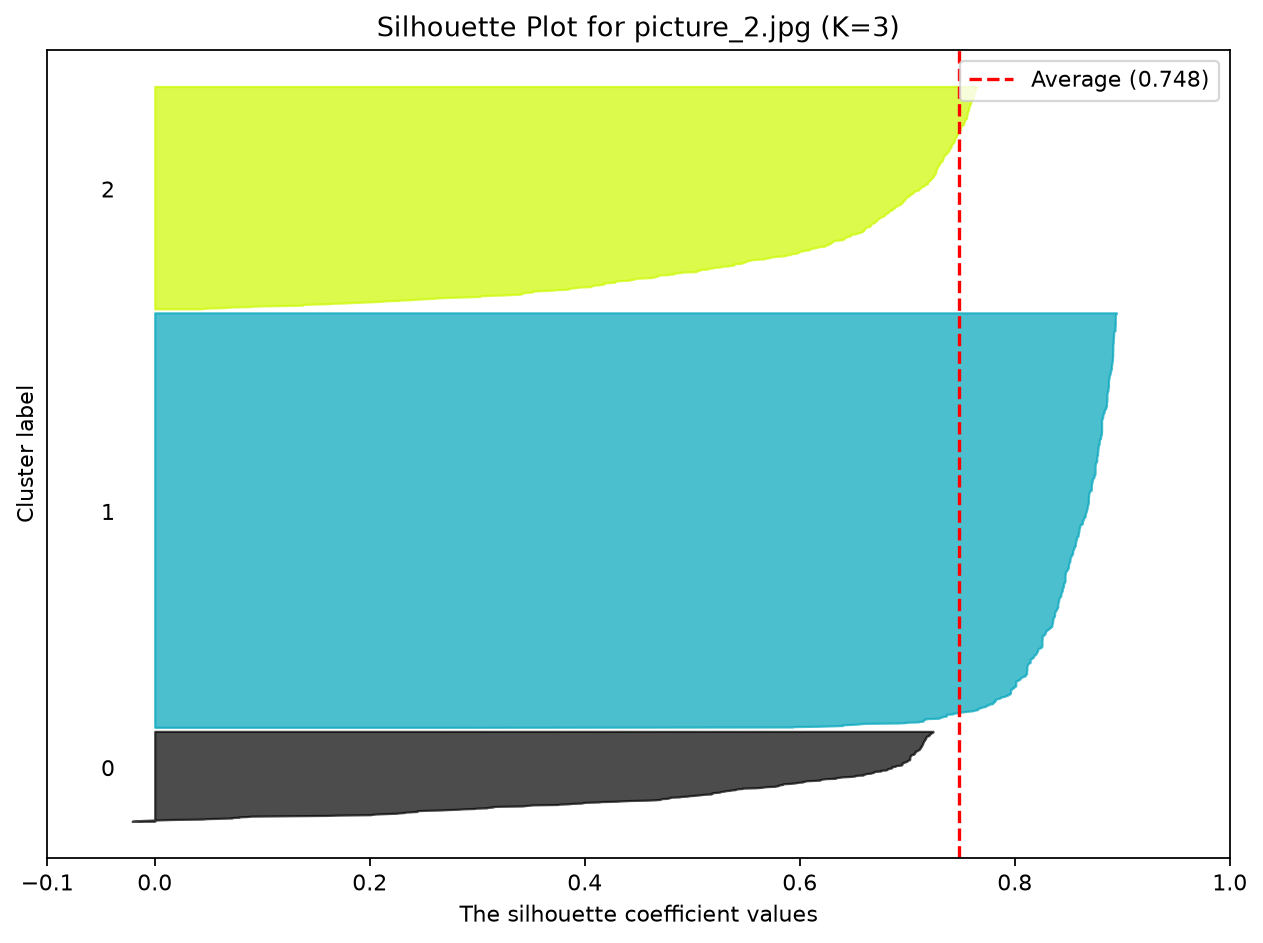
\includegraphics[width=\textwidth]{figures/lab31/silhouette_plot_picture_2_k3.png}
  \caption{Silhouette: Picture 2 at K=3}
\end{figure}
\begin{figure}[H]
  \centering
  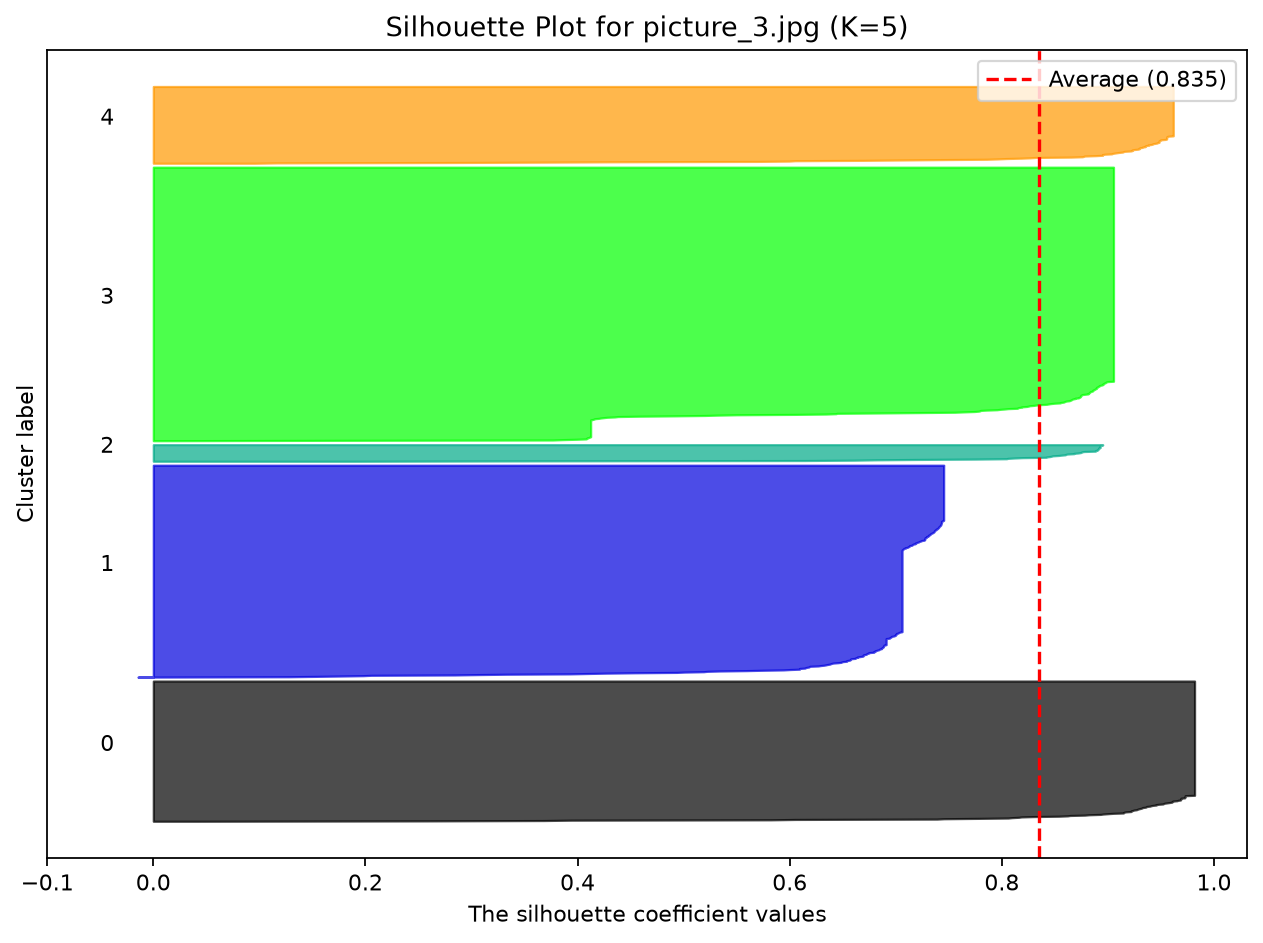
\includegraphics[width=\textwidth]{figures/lab31/silhouette_plot_picture_3_k5.png}
  \caption{Silhouette: Picture 3 at K=5}
\end{figure}
\end{figure}

\subsection{Step 5 — Image Reconstruction}
Each pixel's cluster label (integer 0 to K$-$1) indexes into the \texttt{cluster\_centers\_} table. Centroid coordinates are clipped to [0, 255] (preventing wraparound from float means outside uint8 range) and rounded to uint8 (avoiding systematic truncation bias). Unique-color count after reconstruction should equal K; fewer means two centroids converged to the same color (degenerate cluster).

\begin{figure}[H]\centering
\begin{figure}[H]
  \centering
  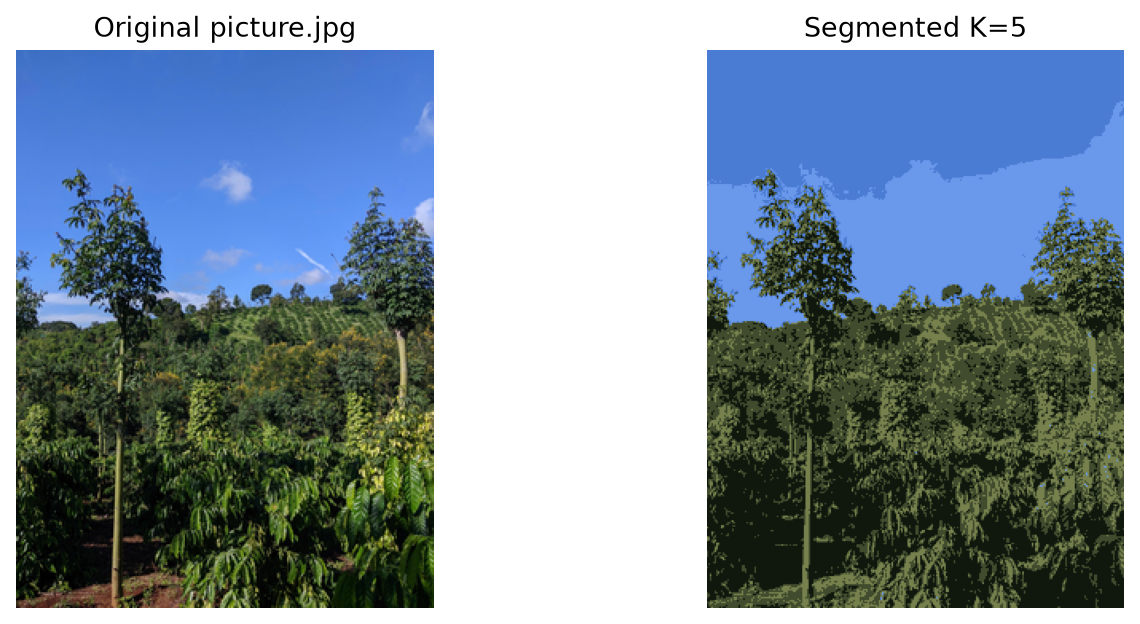
\includegraphics[width=\textwidth]{figures/lab31/original_vs_segmented_picture.png}
  \caption{Original vs. Segmented: Pic 1}
\end{figure}
\begin{figure}[H]
  \centering
  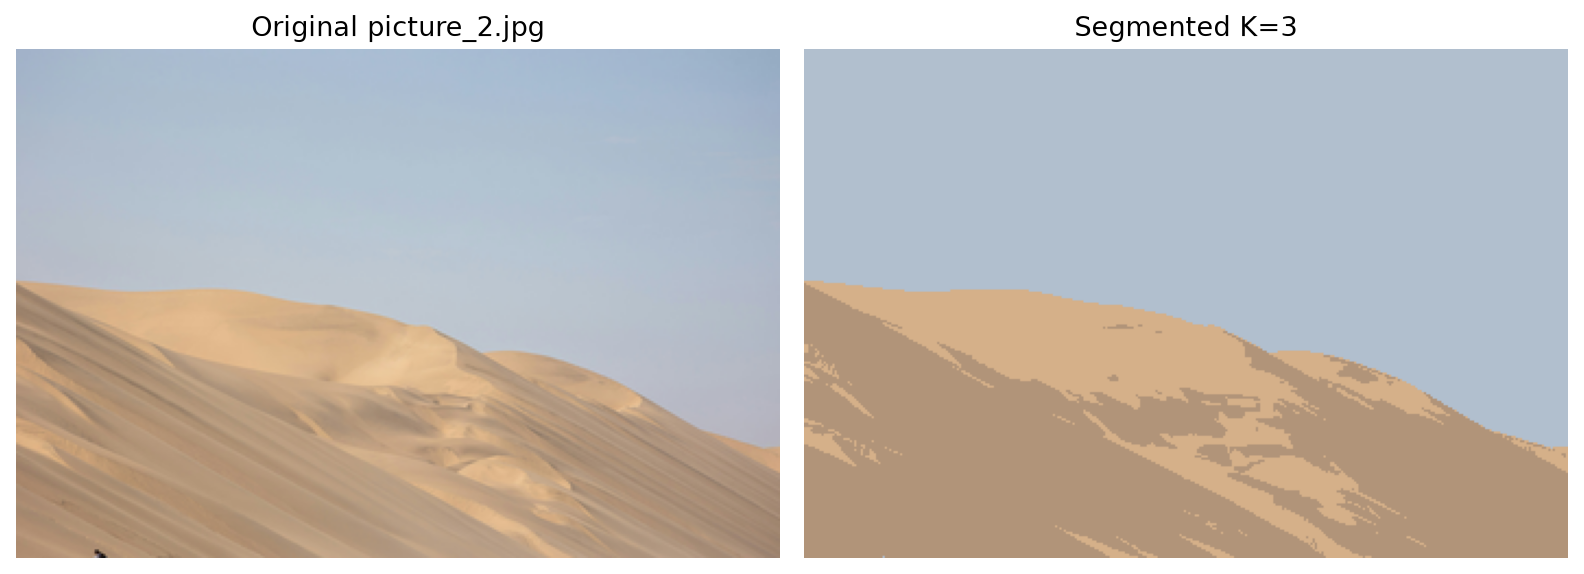
\includegraphics[width=\textwidth]{figures/lab31/original_vs_segmented_picture_2.png}
  \caption{Original vs. Segmented: Pic 2}
\end{figure}
\begin{figure}[H]
  \centering
  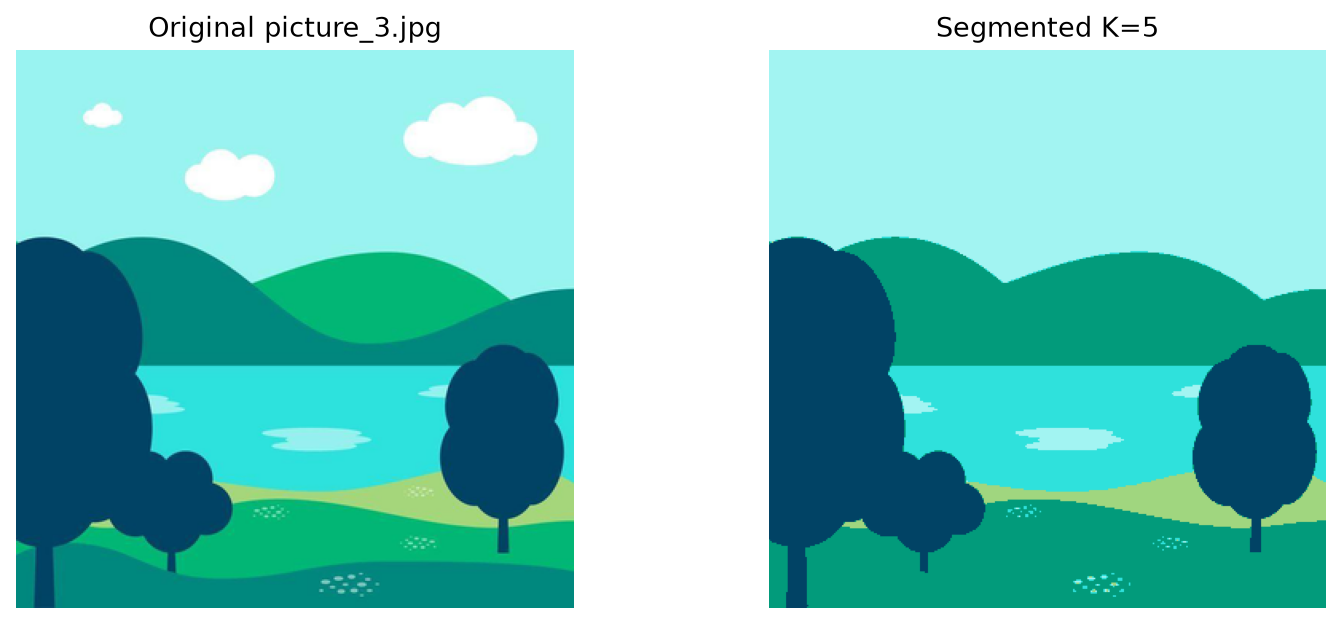
\includegraphics[width=\textwidth]{figures/lab31/original_vs_segmented_picture_3.png}
  \caption{Original vs. Segmented: Pic 3}
\end{figure}
\end{figure}

\begin{figure}[H]\centering
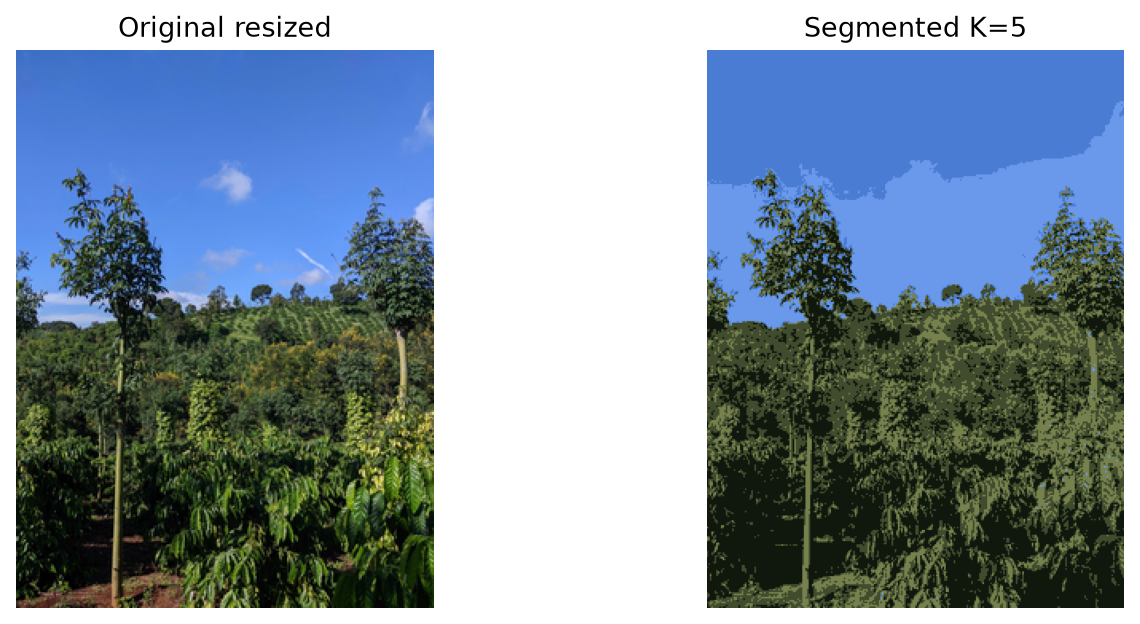
\includegraphics[width=0.78\textwidth]{figures/lab31/original_vs_segmented.png}
\caption{Primary image: original vs. K=5 segmented side-by-side comparison showing color quantization result.}
\end{figure}

\subsection{Step 6 — Visualize Results}
Three diagnostic views:
\begin{enumerate}
  \item \textbf{K-comparison grid:} Original alongside K=2,3,5,8 segmented variants — visual trade-off assessment.
  \item \textbf{Convergence plot:} Inertia per iteration, all K on one plot. Monotonic descent flattening within 10–20 iterations = healthy. Spikes = empty cluster re-initialization.
  \item \textbf{Centroid color palette:} Each cluster's centroid rendered as a swatch. Muddy swatches = centroid averaging many dissimilar colors; visually identical swatches = degenerate clusters.
\end{enumerate}

\subsection{Step 7 — Color Space Comparison}
K-Means is fit in RGB, HSV, and LAB at each image's optimal K. Inertia values are \textbf{not directly comparable} across spaces (different coordinate scales) — compare convergence stability and visual quality instead. LAB often groups shadowed pixels with their lit counterparts of the same material (e.g., a shadowed green leaf stays in ``green'' rather than being swept into ``dark'').

\subsection{Step 8 — Sklearn Sanity Check}
\texttt{sklearn.cluster.KMeans} (with \texttt{n\_init=10}) is run at the optimal K. Manual vs. sklearn inertia should agree within $\pm 5\%$. Differences arise from random-pixel vs. k-means++ initialization, floating-point accumulation order, and empty-cluster handling strategies. Consistently higher manual inertia ($>10\%$) suggests a bug; lower inertia indicates a fortunate initialization.

\subsection{Step 9 — Output Verification}
Every expected artifact is enumerated and checked for existence — resized images, segmented images at all K, comparison grids, convergence/silhouette/elbow plots, color palettes, and the metrics CSV. Output: \texttt{OK} or \texttt{MISSING} per path.

\section{Results and Analysis}

\begin{resultbox}
\textbf{Selected K = 5} — best balance of visual simplicity and scene detail.\\
Silhouette: 0.5180 (well-separated color regions). Convergence: 30 iterations.
\end{resultbox}

\begin{table}[H]
\centering\rowcolors{2}{tablerow}{white}
\begin{tabular}{c c c c}
\toprule\rowcolor{tablehead!80}\color{white}\textbf{K} &\color{white}\textbf{Inertia} &\color{white}\textbf{Silhouette} &\color{white}\textbf{Iters}\\
\midrule
2 & 261,719,604 & 0.6894 & 6\\
3 & 126,918,501 & 0.6210 & 16\\
\rowcolor{greenaccent!15}\textbf{5} & \textbf{69,047,213} & \textbf{0.5180} & \textbf{30}\\
8 & 41,557,214 & 0.4919 & 49\\
\bottomrule
\end{tabular}
\caption{Segmentation metrics across K values}
\end{table}

\begin{figure}[H]\centering
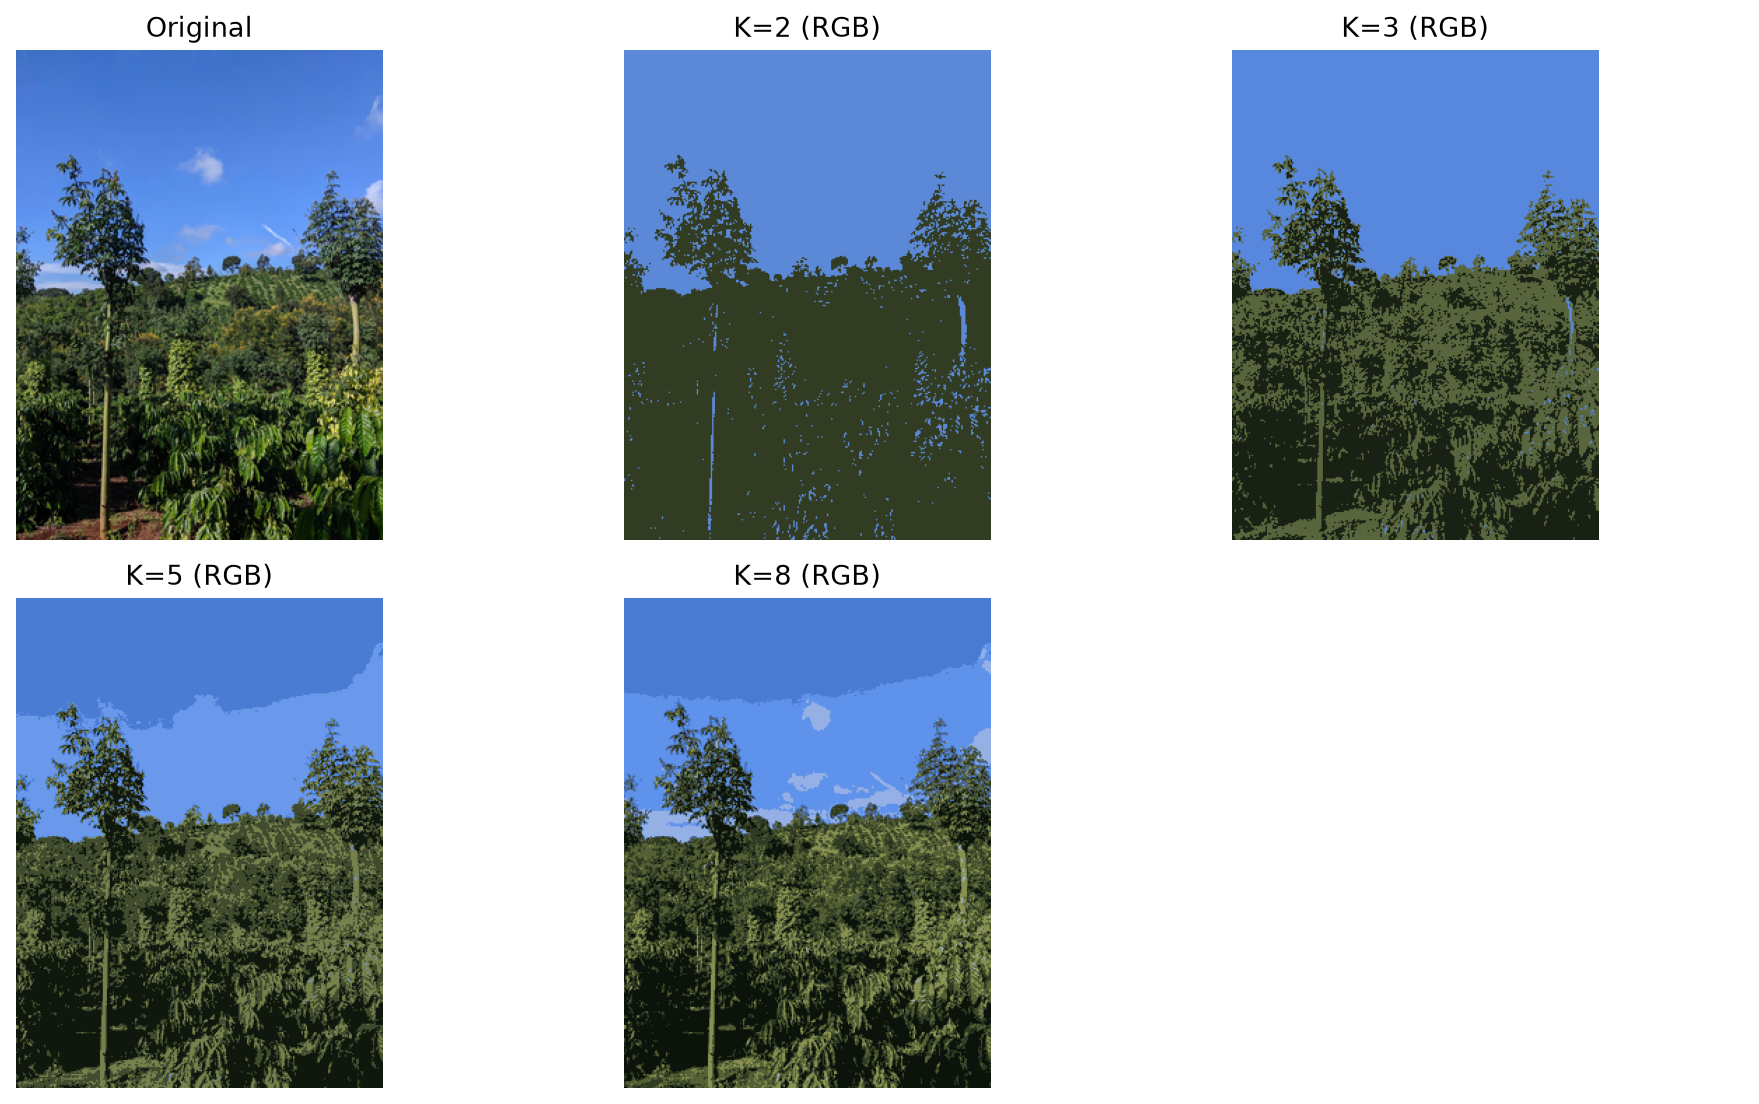
\includegraphics[width=0.9\textwidth]{figures/lab31/k_comparison_grid_picture.png}
\caption{K-comparison grid: original image alongside K=2,3,5,8 segmentations. K=2 produces stark posterization; K=8 preserves near-original detail.}
\end{figure}

\begin{figure}[H]\centering
\begin{figure}[H]
  \centering
  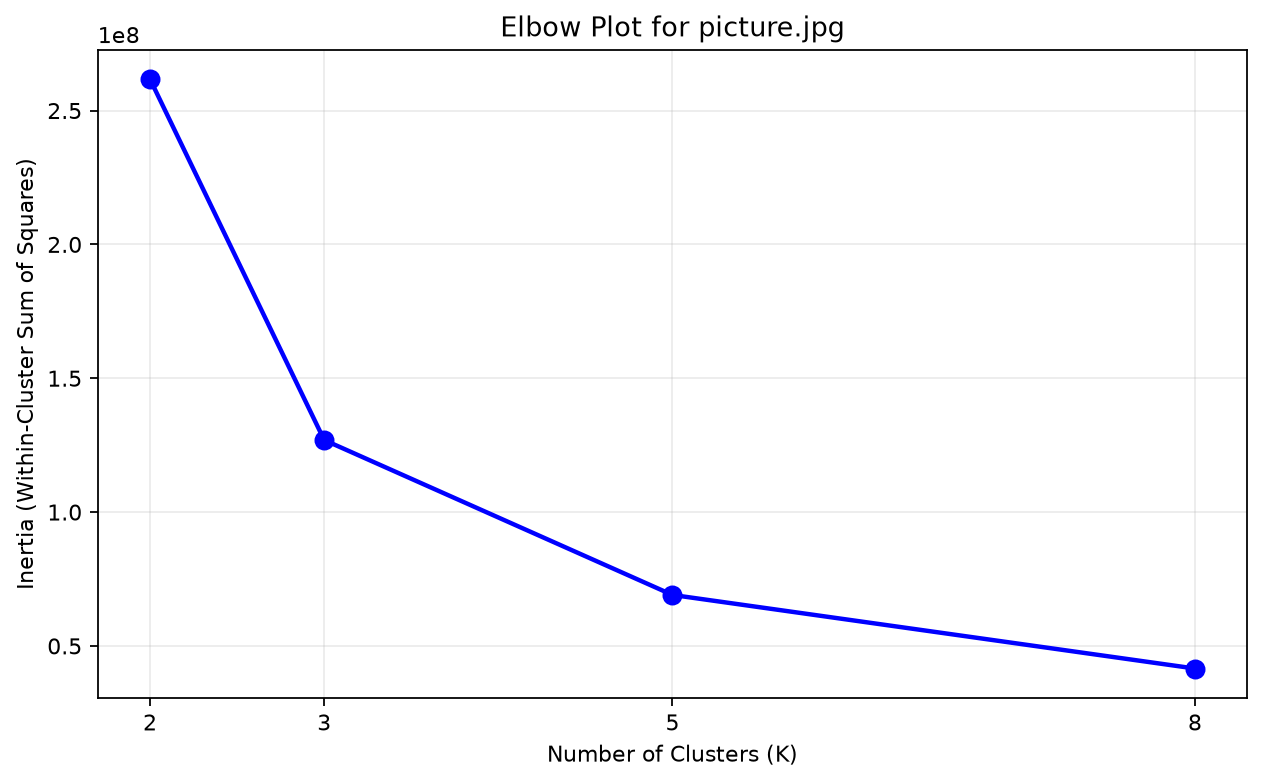
\includegraphics[width=\textwidth]{figures/lab31/elbow_plot_picture.png}
  \caption{Elbow: inertia vs. K — bend at K=3–5}
\end{figure}
\begin{figure}[H]
  \centering
  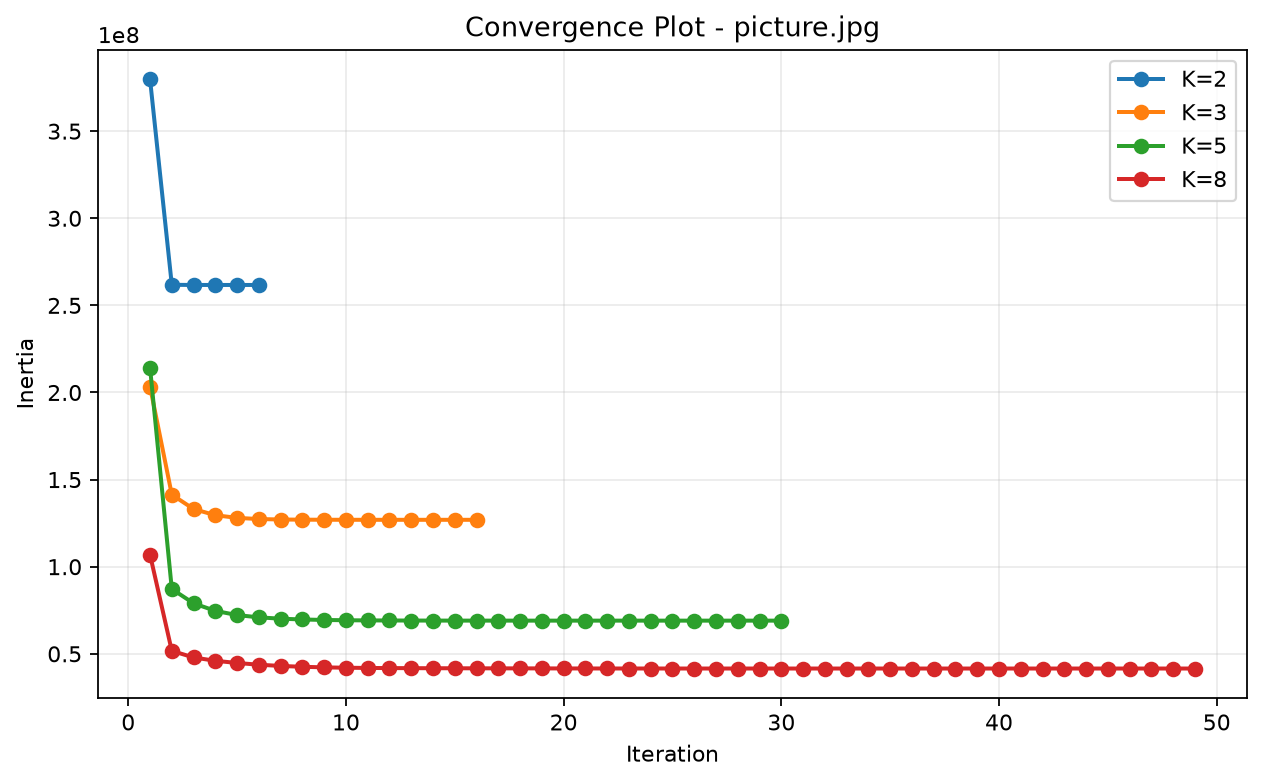
\includegraphics[width=\textwidth]{figures/lab31/convergence_plot_picture.png}
  \caption{Convergence: inertia decreases monotonically}
\end{figure}
\end{figure}

\begin{figure}[H]\centering
\begin{figure}[H]
  \centering
  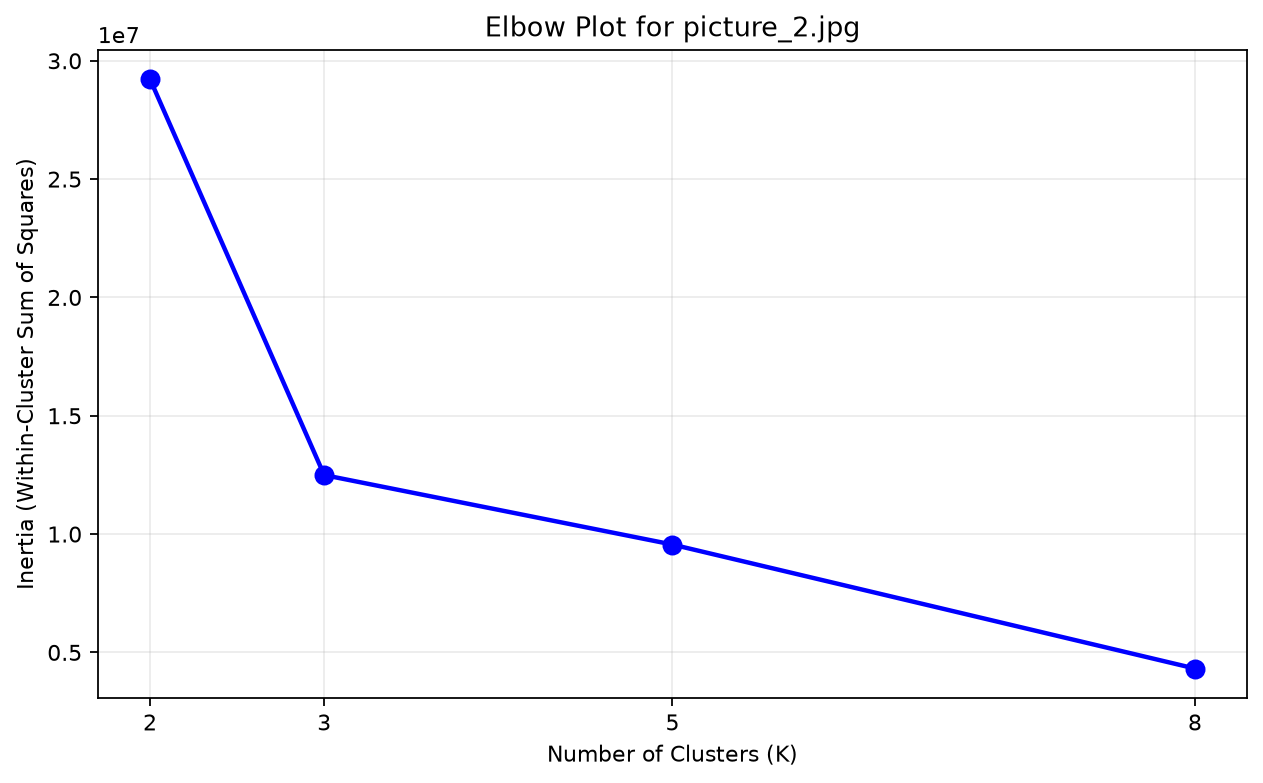
\includegraphics[width=\textwidth]{figures/lab31/elbow_plot_picture_2.png}
  \caption{Elbow curve: Picture 2}
\end{figure}
\begin{figure}[H]
  \centering
  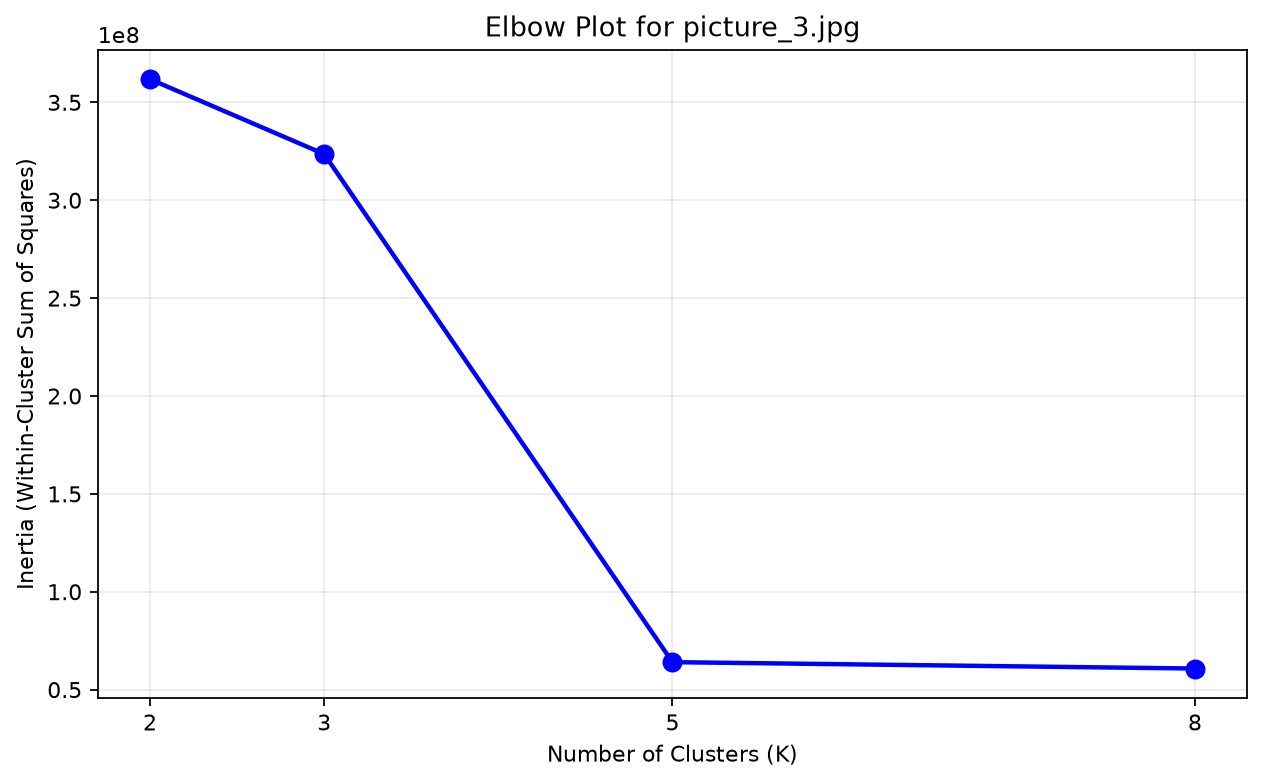
\includegraphics[width=\textwidth]{figures/lab31/elbow_plot_picture_3.png}
  \caption{Elbow curve: Picture 3}
\end{figure}\
\vspace{4pt}
\begin{figure}[H]
  \centering
  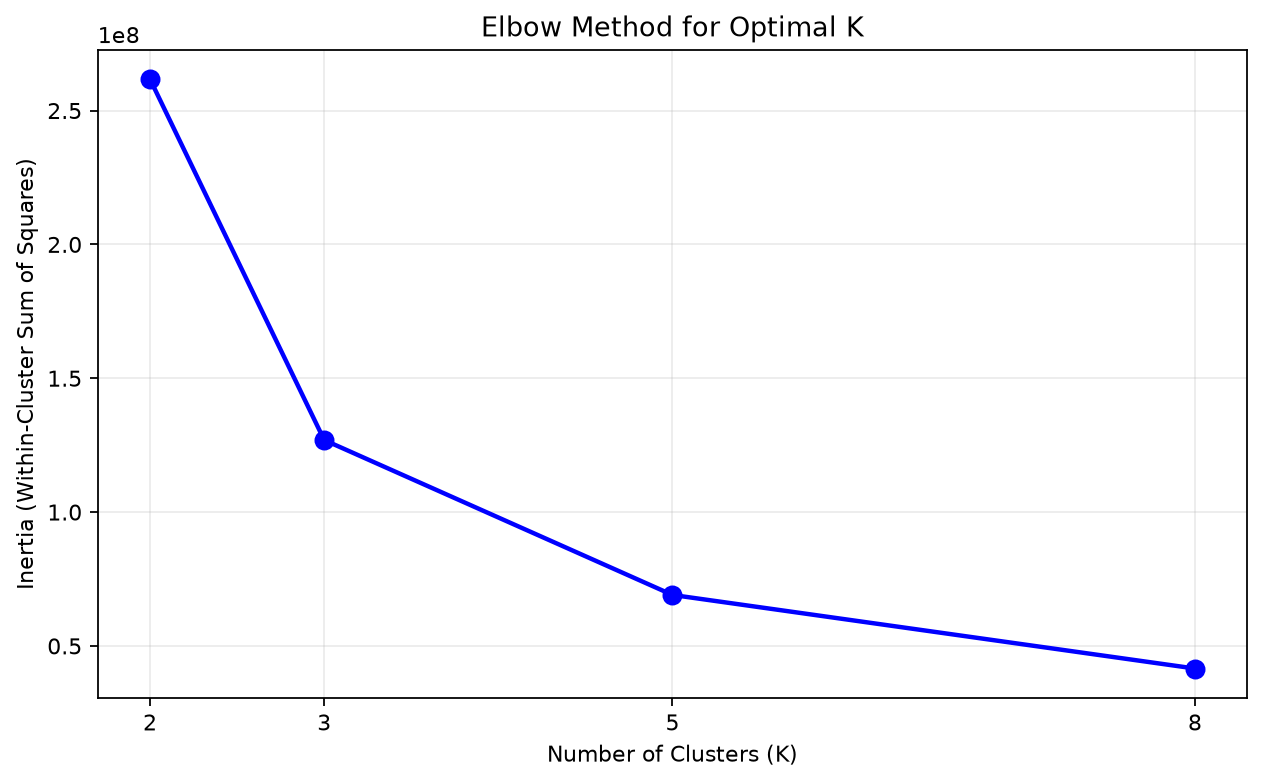
\includegraphics[width=\textwidth]{figures/lab31/elbow_plot.png}
  \caption{Elbow curve: all pictures}
\end{figure}
\begin{figure}[H]
  \centering
  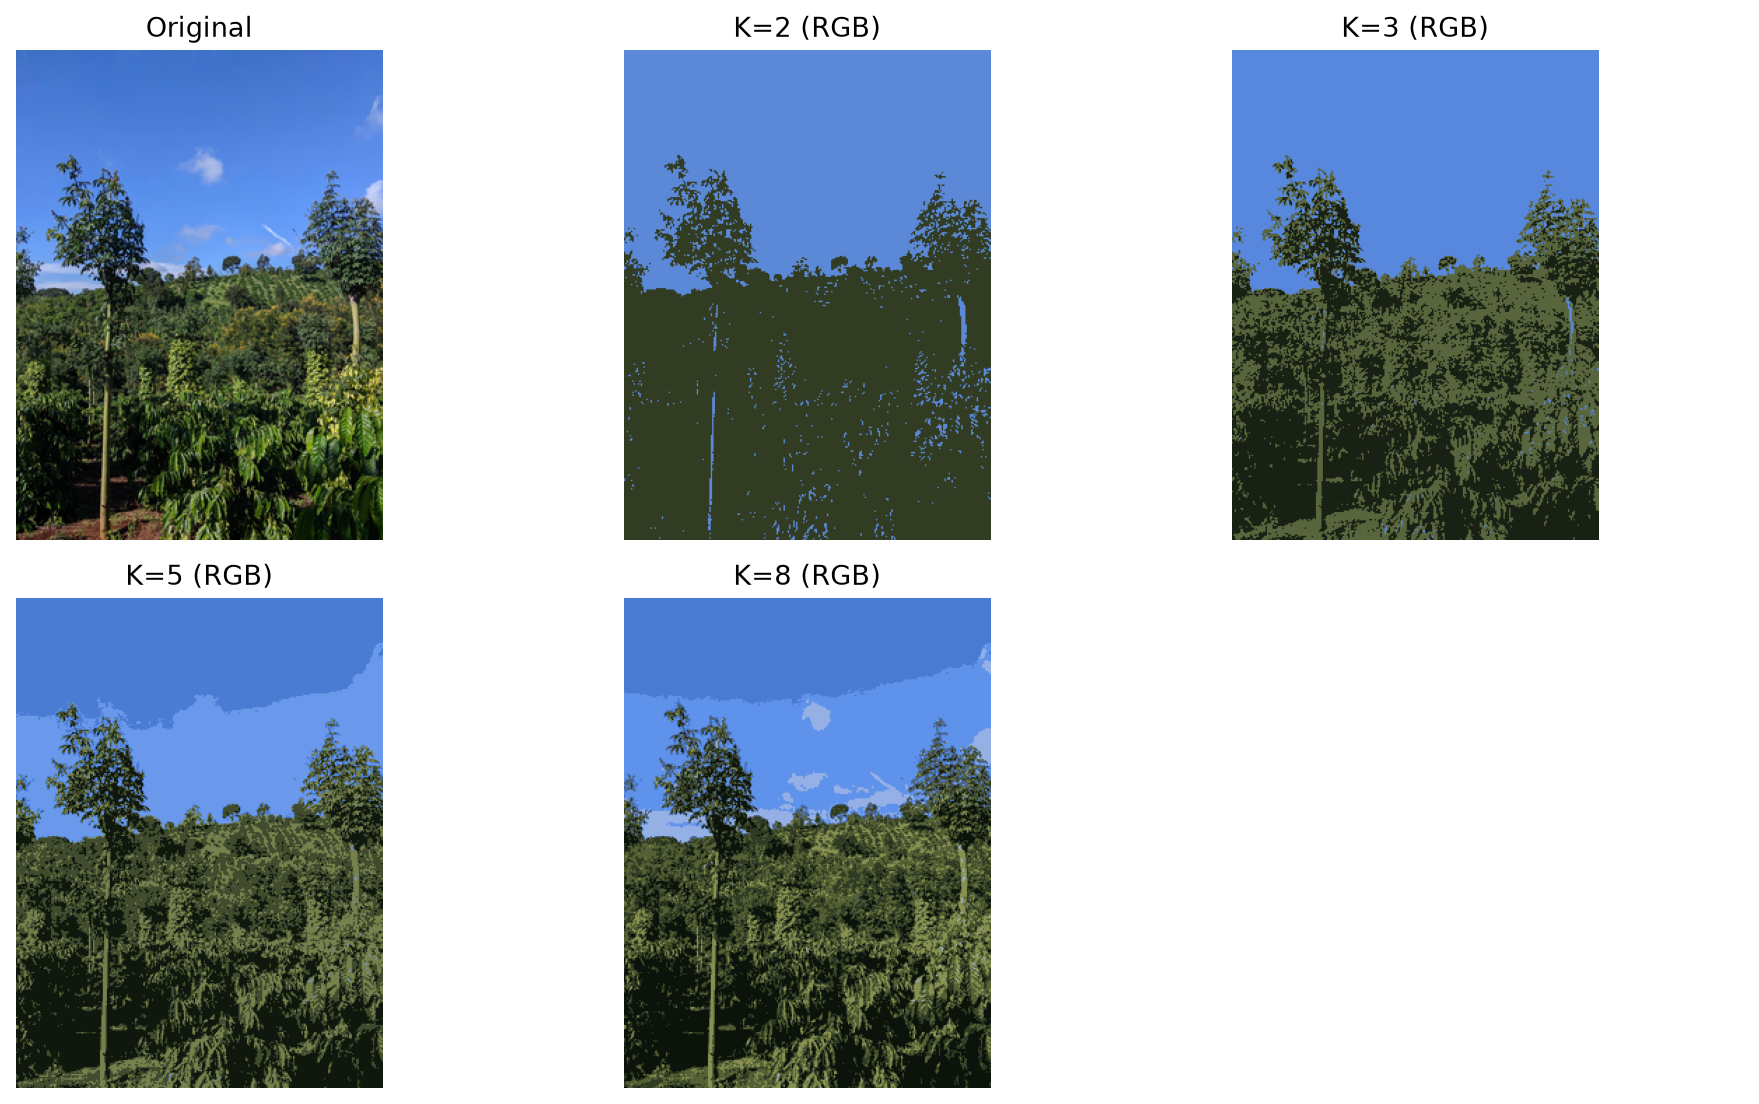
\includegraphics[width=\textwidth]{figures/lab31/k_comparison_grid.png}
  \caption{K-comparison grid}
\end{figure}
\end{figure}

\begin{figure}[H]\centering
\begin{figure}[H]
  \centering
  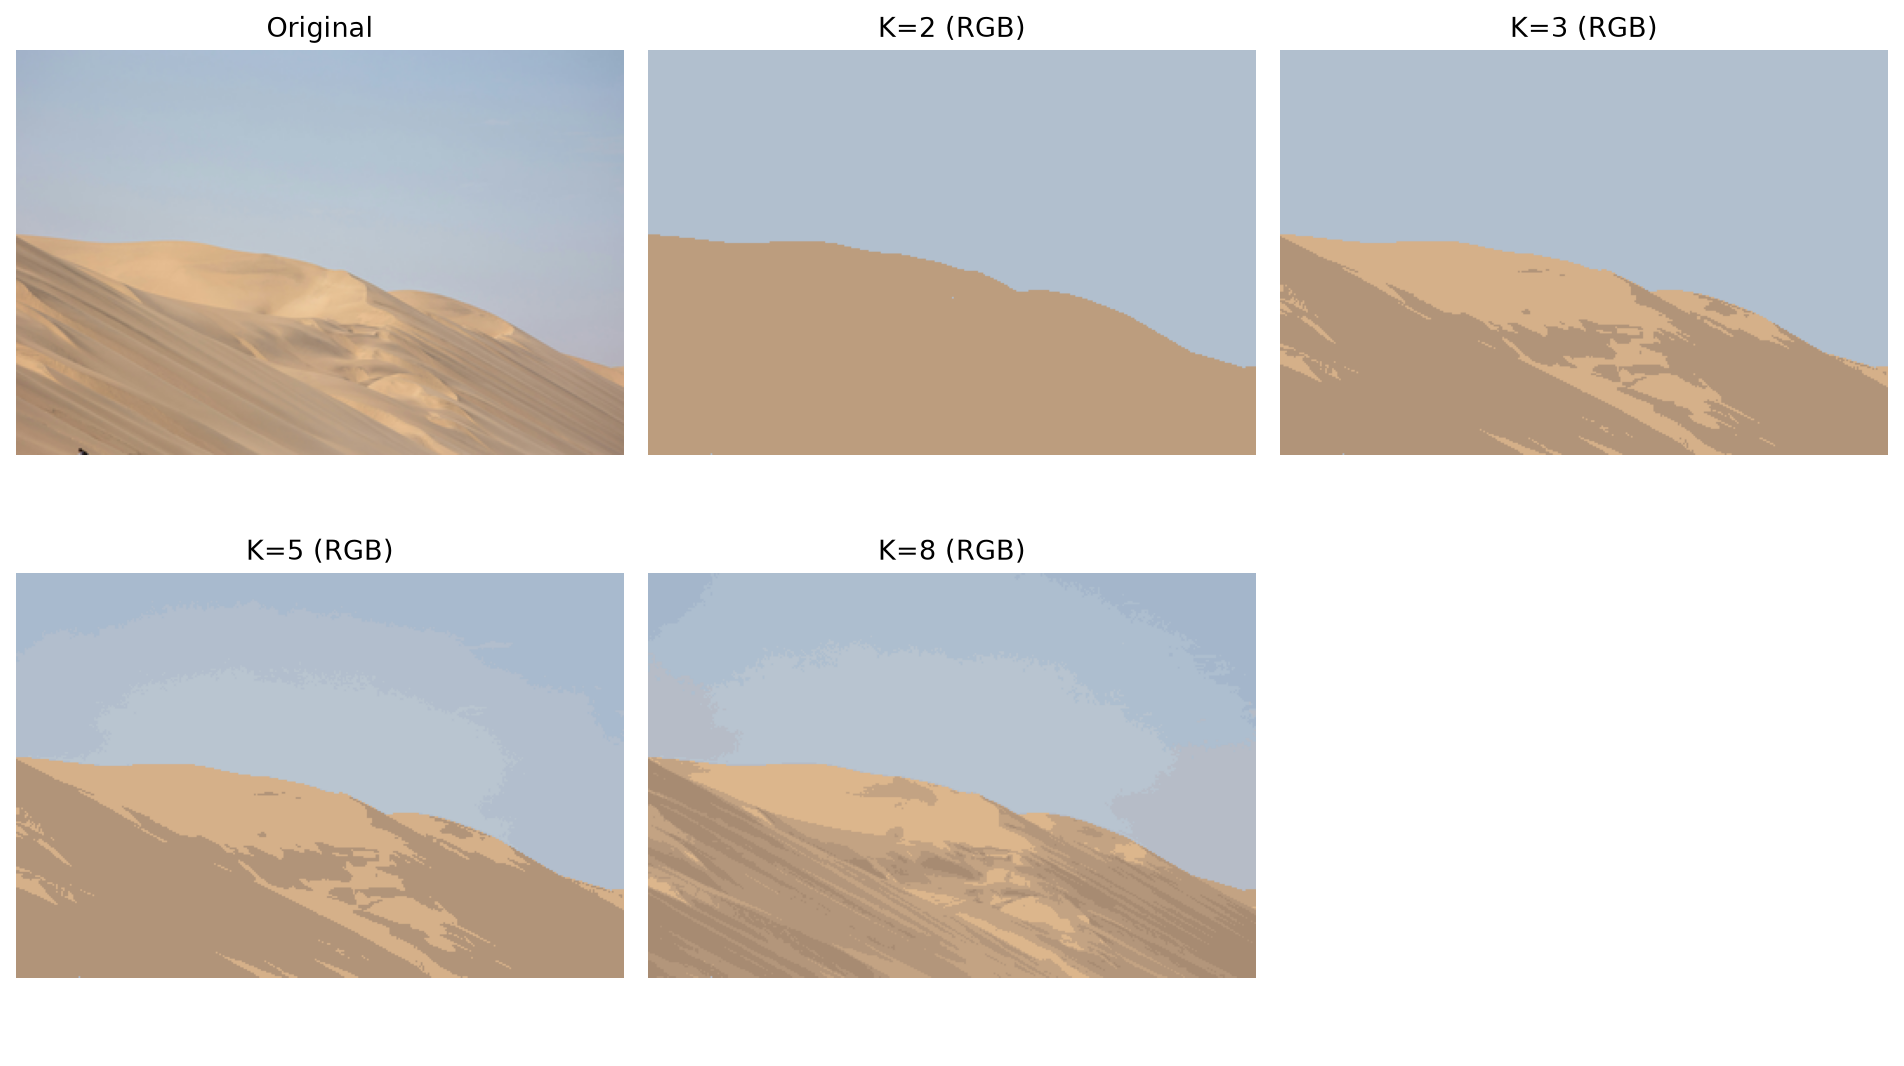
\includegraphics[width=\textwidth]{figures/lab31/k_comparison_grid_picture_2.png}
  \caption{K-comparison: Picture 2}
\end{figure}
\begin{figure}[H]
  \centering
  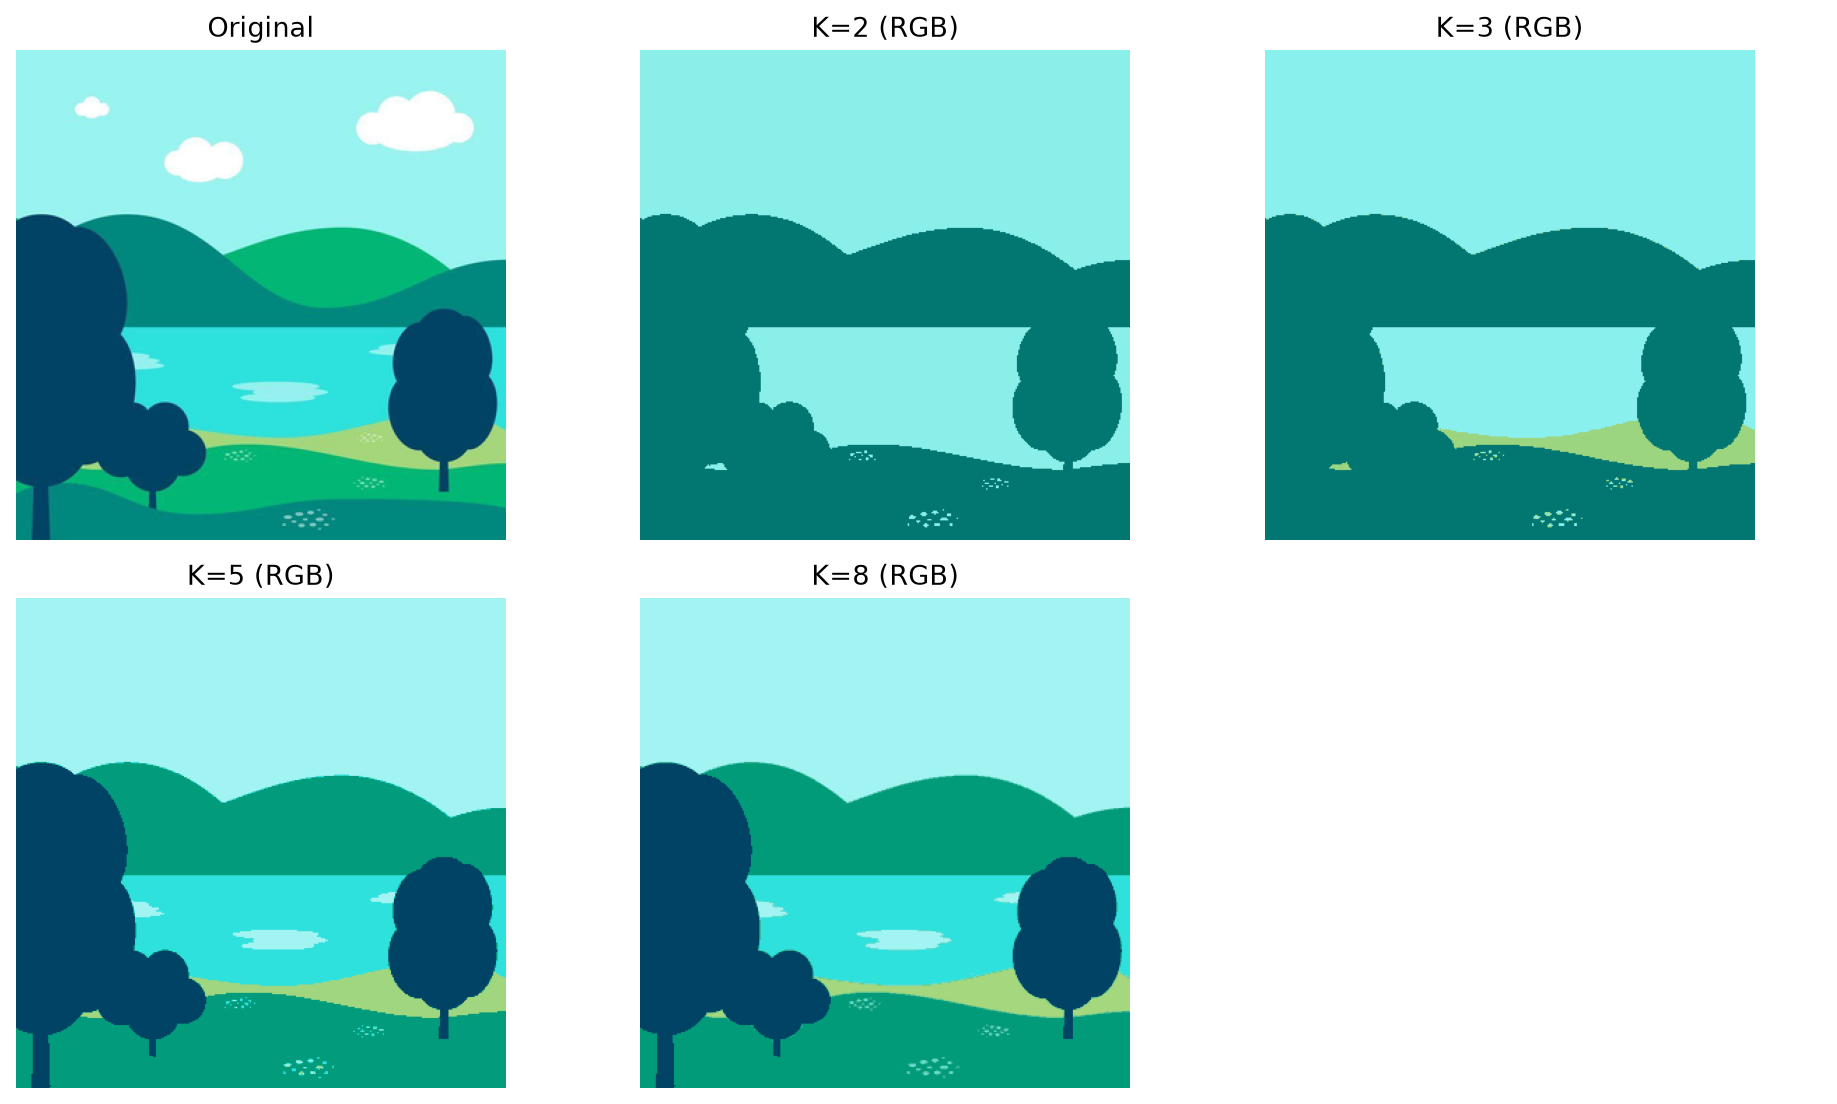
\includegraphics[width=\textwidth]{figures/lab31/k_comparison_grid_picture_3.png}
  \caption{K-comparison: Picture 3}
\end{figure}
\end{figure}

\begin{figure}[H]\centering
\begin{figure}[H]
  \centering
  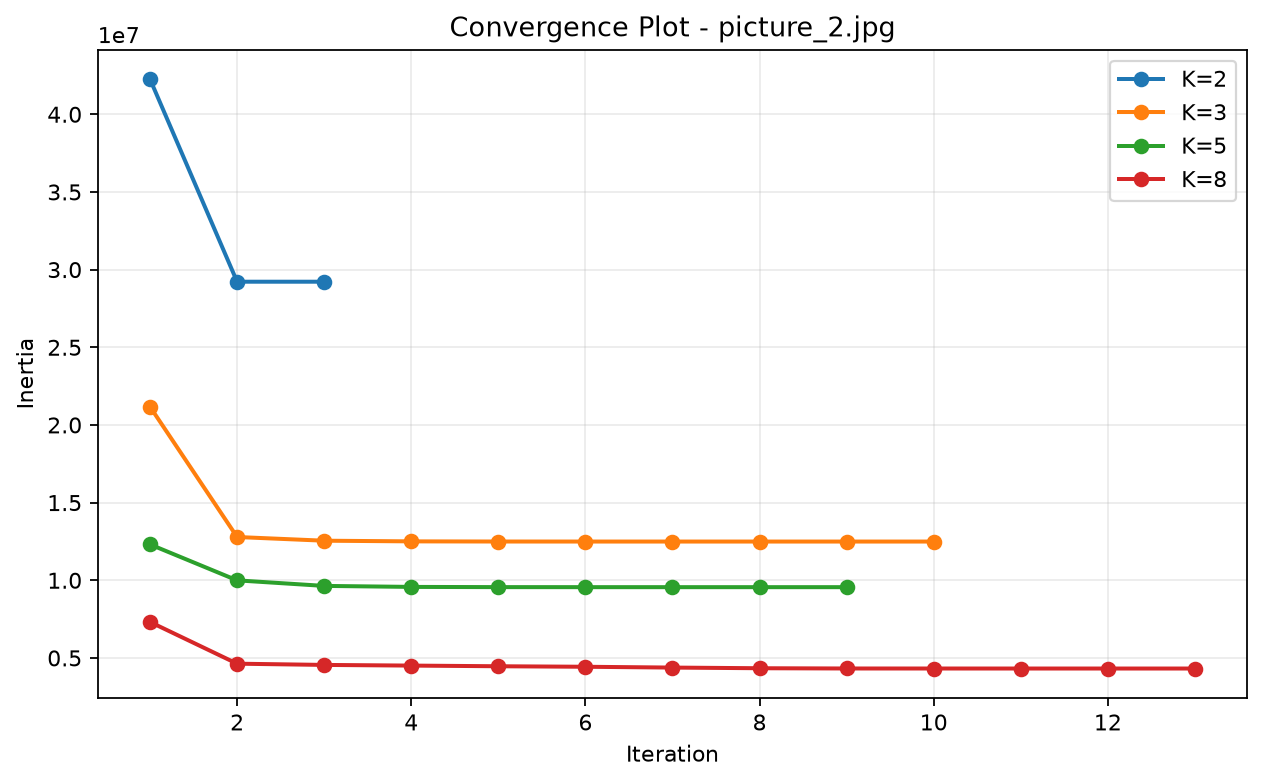
\includegraphics[width=\textwidth]{figures/lab31/convergence_plot_picture_2.png}
  \caption{Convergence: Picture 2}
\end{figure}
\begin{figure}[H]
  \centering
  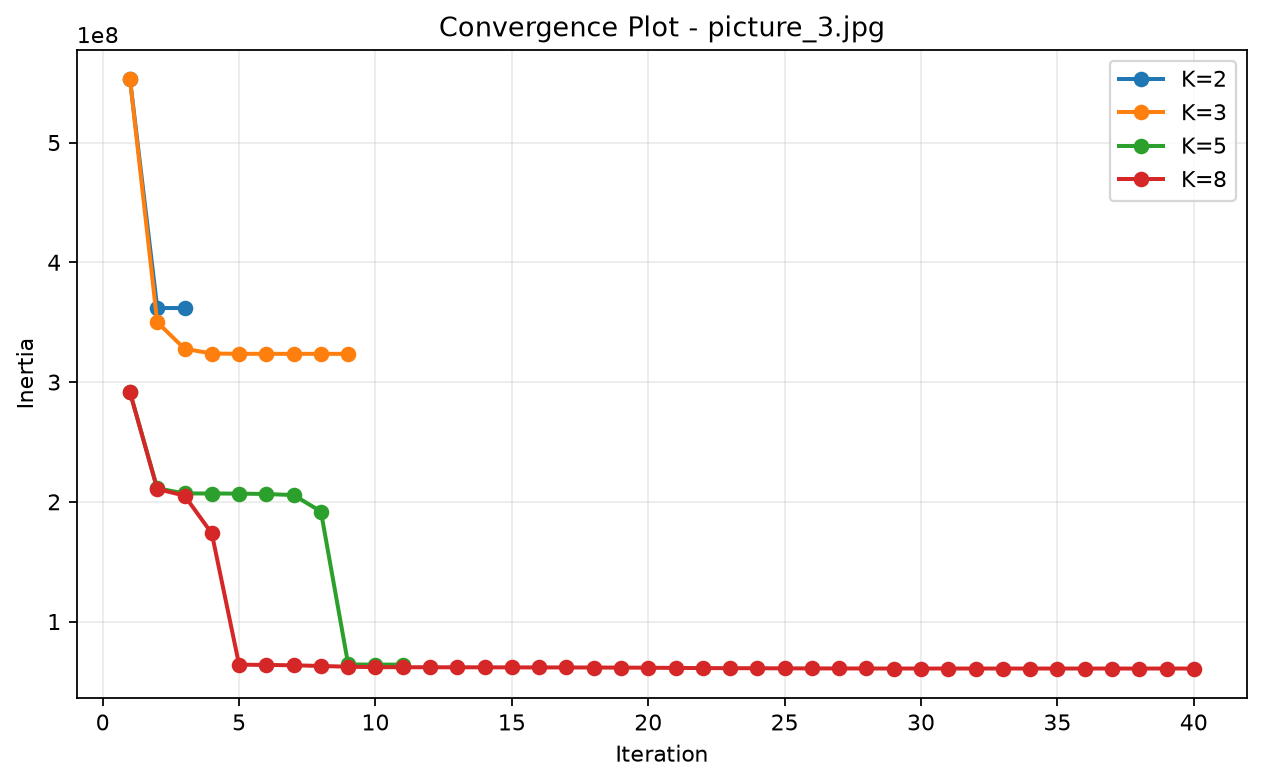
\includegraphics[width=\textwidth]{figures/lab31/convergence_plot_picture_3.png}
  \caption{Convergence: Picture 3}
\end{figure}\
\vspace{4pt}
\begin{figure}[H]
  \centering
  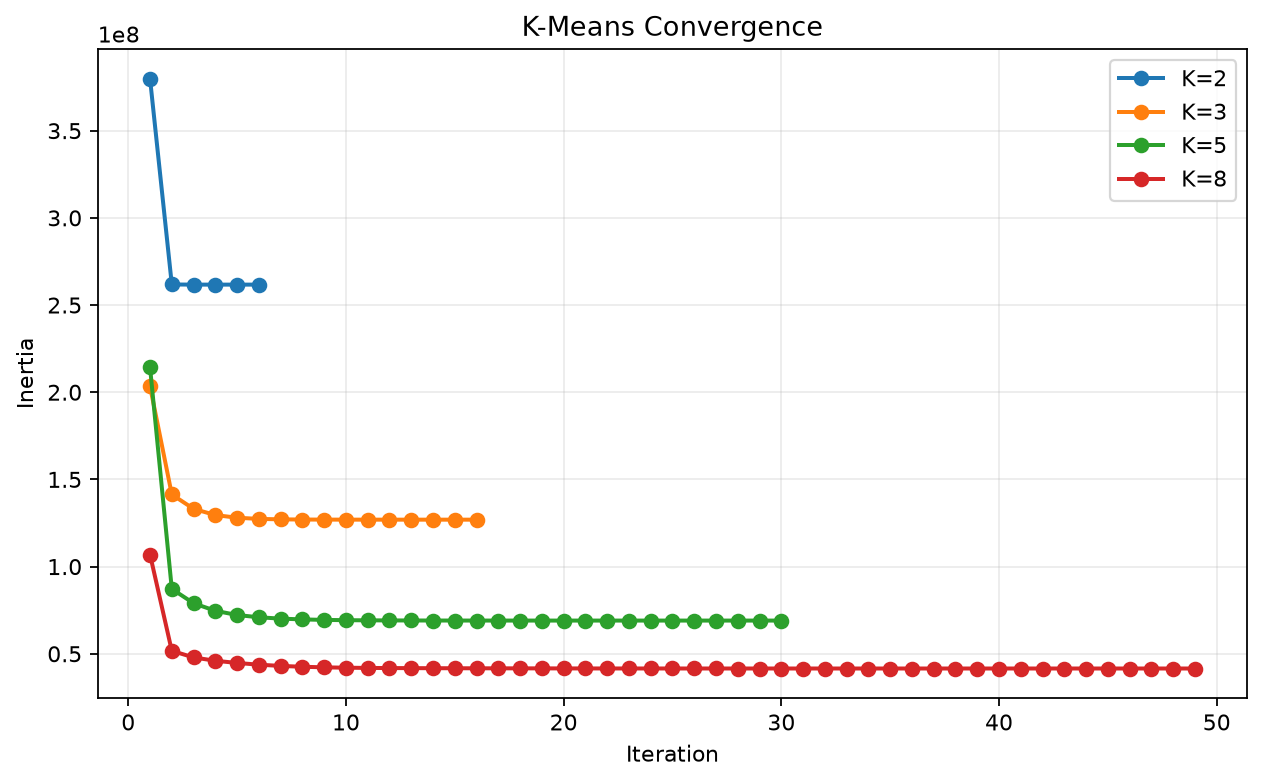
\includegraphics[width=\textwidth]{figures/lab31/convergence_plot.png}
  \caption{Convergence: all pictures}
\end{figure}
\begin{figure}[H]
  \centering
  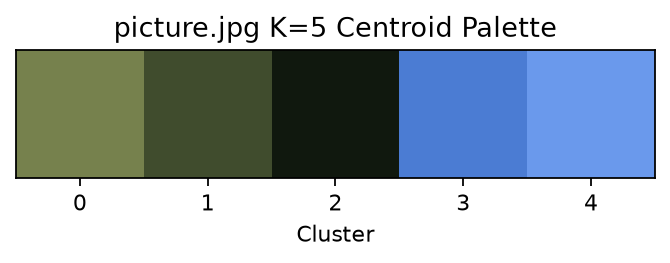
\includegraphics[width=\textwidth]{figures/lab31/color_palette_picture_k5.png}
  \caption{Color palette at K=5}
\end{figure}
\end{figure}

\begin{figure}[H]\centering
\begin{figure}[H]
  \centering
  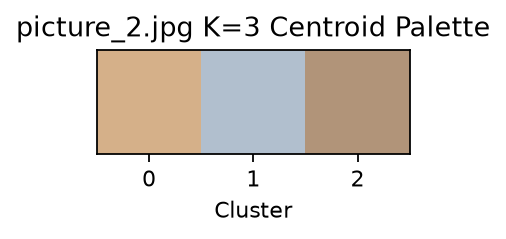
\includegraphics[width=\textwidth]{figures/lab31/color_palette_picture_2_k3.png}
  \caption{Palette: Picture 2, K=3}
\end{figure}
\begin{figure}[H]
  \centering
  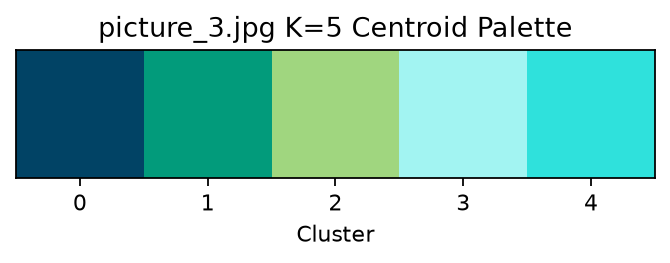
\includegraphics[width=\textwidth]{figures/lab31/color_palette_picture_3_k5.png}
  \caption{Palette: Picture 3, K=5}
\end{figure}\
\vspace{4pt}
\begin{figure}[H]
  \centering
  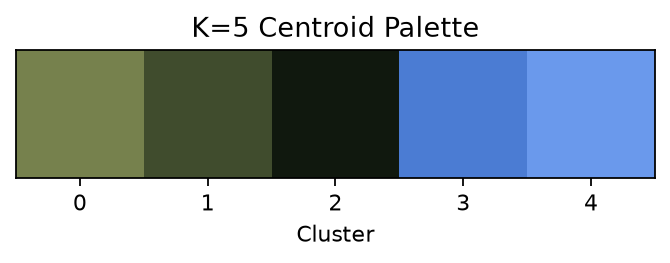
\includegraphics[width=\textwidth]{figures/lab31/color_palette_k5.png}
  \caption{Color palette K=5 detail}
\end{figure}
\end{figure}

\begin{notebox}
\textbf{Always use silhouette alongside elbow for choosing K.} Inertia is guaranteed to decrease with more clusters — it can never penalize over-segmentation. Silhouette can penalize fragmented clusters by detecting overlap. The convergence plot shows monotonic descent for all K, confirming healthy optimization. K=5 is selected because the elbow flattens after this point and silhouette remains strong (0.52) without excessive iterations.
\end{notebox}

% ═══════════════════════════════════════════════════════════════
\chapter{Lab 04 — California Housing Price Prediction}
\label{ch:lab04}
% ═══════════════════════════════════════════════════════════════

\section{Problem Definition}

\begin{problembox}
Predict \textbf{median house value} (USD) from census-block features using three regression models built \textit{from scratch} in pure NumPy. The dataset is the classic California Housing dataset (1990 census). Success criteria: \textbf{RMSE $< \$75{,}000$}, \textbf{R² $> 0.60$}, \textbf{MAPE $< 30\%$}. Every component — gradient descent, backpropagation, histogram-based tree splitting — is implemented from scratch without high-level ML libraries.
\end{problembox}

\subsection{Dataset}
\begin{itemize}
  \item \textbf{Source:} California Housing (1990 census), 20,640 rows, 10 columns.
  \item \textbf{Features:} 8 numeric (longitude, latitude, housing\_median\_age, total\_rooms, total\_bedrooms, population, households, median\_income) + 1 categorical (ocean\_proximity, 5 levels).
  \item \textbf{Target:} \texttt{median\_house\_value}, capped at \$500,006.
  \item \textbf{Split:} Stratified 80/20 on binned \texttt{median\_income} — 16,512 train, 4,128 test.
\end{itemize}

\section{Complete Workflow}

\subsection{Step 1 — Setup and Load Data}
Key libraries imported, project root resolved, \texttt{src/lab04} added to \texttt{sys.path} for custom module access. Raw CSV loaded: 20,640 rows, 10 columns. \texttt{d.head()}, \texttt{.info()}, \texttt{.describe()} provide the first look.

\subsection{Step 2 — Exploratory Data Analysis (8 Sub-steps)}

\subsubsection{2.1 — Descriptive Statistics}
\texttt{df.describe()} confirms: \texttt{median\_house\_value} capped at \$500,006; \texttt{total\_rooms}, \texttt{total\_bedrooms}, \texttt{population} are right-skewed (large 75th-percentile–max gaps). \texttt{ocean\_proximity} value counts show 5 categories — if any have $<30$ samples, merge with neighbors.

\subsubsection{2.2 — Missing Values}
Only \texttt{total\_bedrooms} has missing data ($\sim$1.5\%). Median imputation is safe for any column with $<10\%$ missing. \texttt{eda.plot\_missing\_values()} renders a bar chart.

\begin{figure}[H]\centering
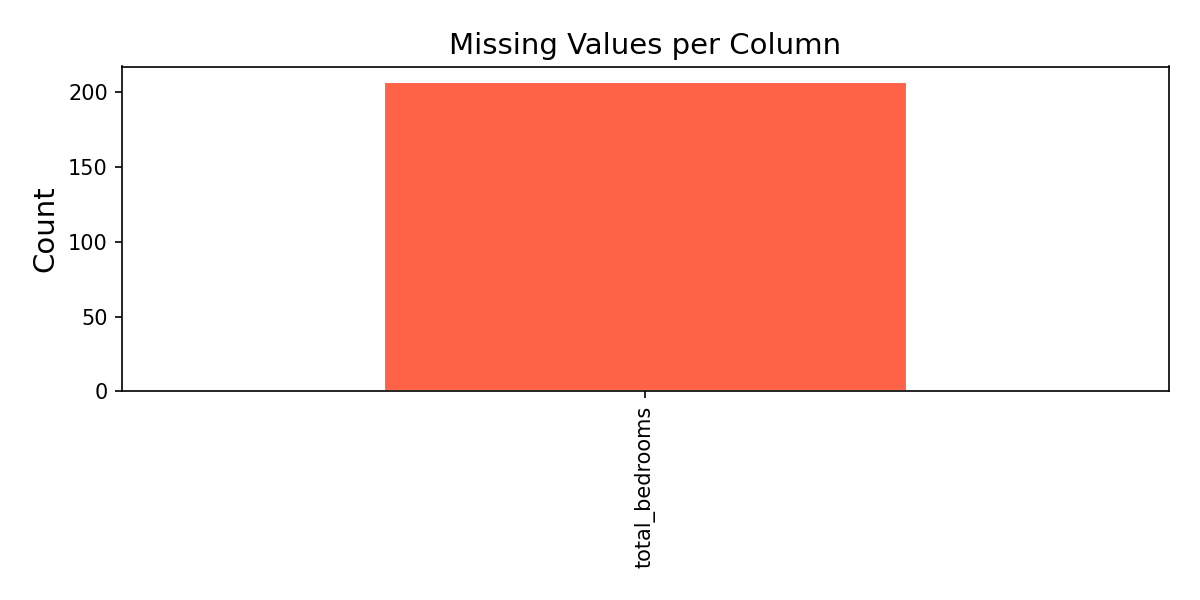
\includegraphics[width=0.72\textwidth]{figures/lab04/eda_01_missing_values.png}
\caption{Missing values bar chart — only \texttt{total\_bedrooms} shows gaps ($\sim$1.5\%), all other columns are complete.}
\end{figure}

\subsubsection{2.3 — Feature Distributions}
Histograms for all numeric features. Right-skewed count features (rooms, population) are candidates for $\log_{1p}$ transform. Target histogram shows a plateau/spike at \$500,006 — the artificial cap. If $>5\%$ of values hit the cap, consider treating this as censored regression.

\begin{figure}[H]\centering
\begin{figure}[H]
  \centering
  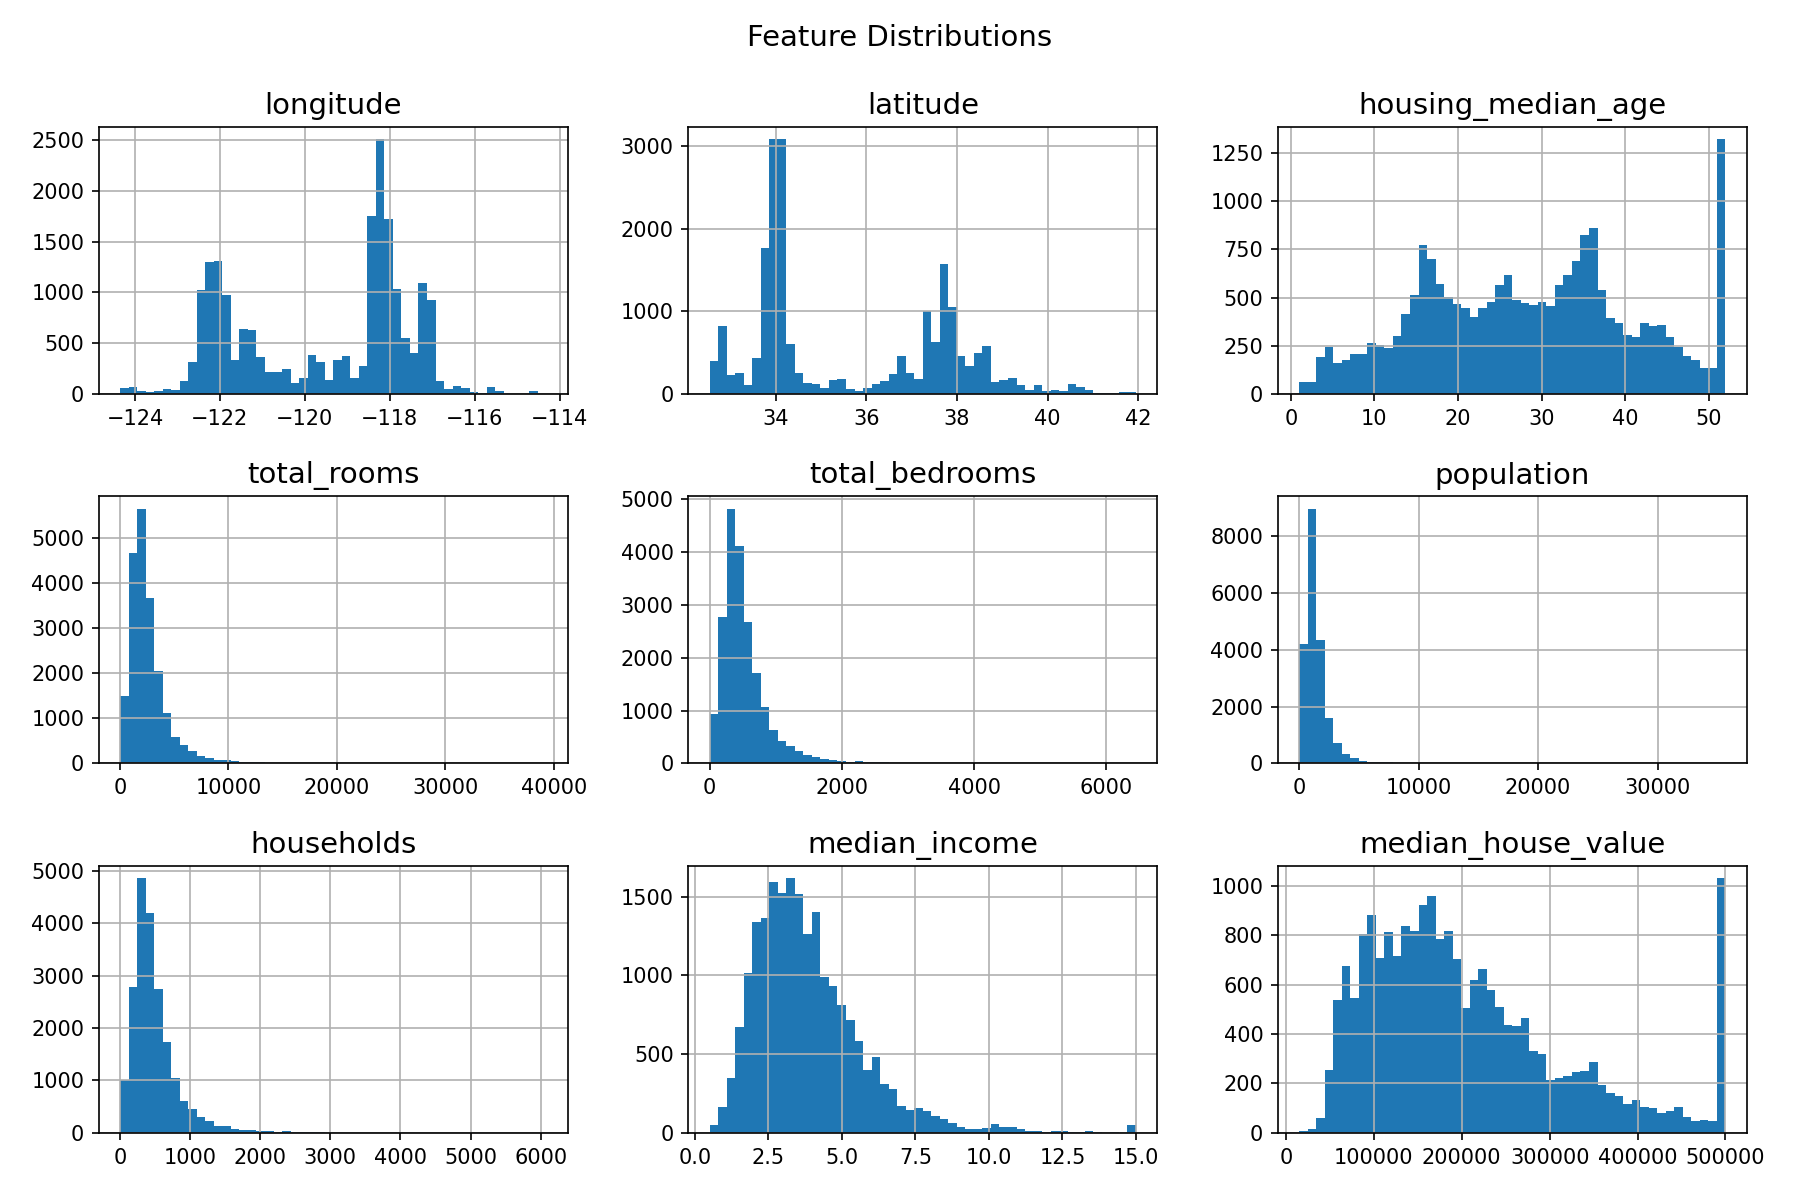
\includegraphics[width=\textwidth]{figures/lab04/eda_02_feature_distributions.png}
  \caption{Feature distributions}
\end{figure}
\begin{figure}[H]
  \centering
  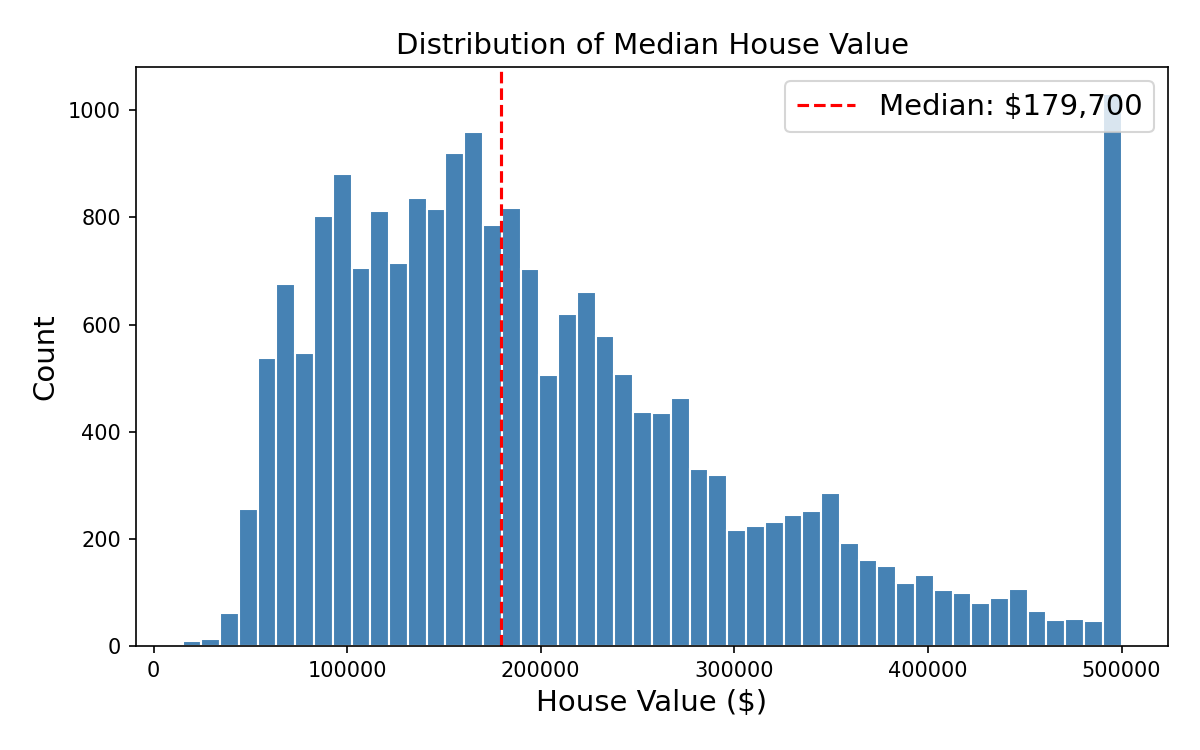
\includegraphics[width=\textwidth]{figures/lab04/eda_03_target_distribution.png}
  \caption{Target distribution}
\end{figure}
\end{figure}

\subsubsection{2.4 — Geographic Distribution}
\texttt{eda.plot\_geographic\_distribution()} renders longitude vs. latitude with color-coded prices. Coastal areas (Los Angeles, San Francisco Bay) command higher prices; inland blocks form a distinct low-price cluster. \textbf{Location is a strong, non-linear predictor} — linear models will struggle with spatial patterns.

\begin{figure}[H]\centering
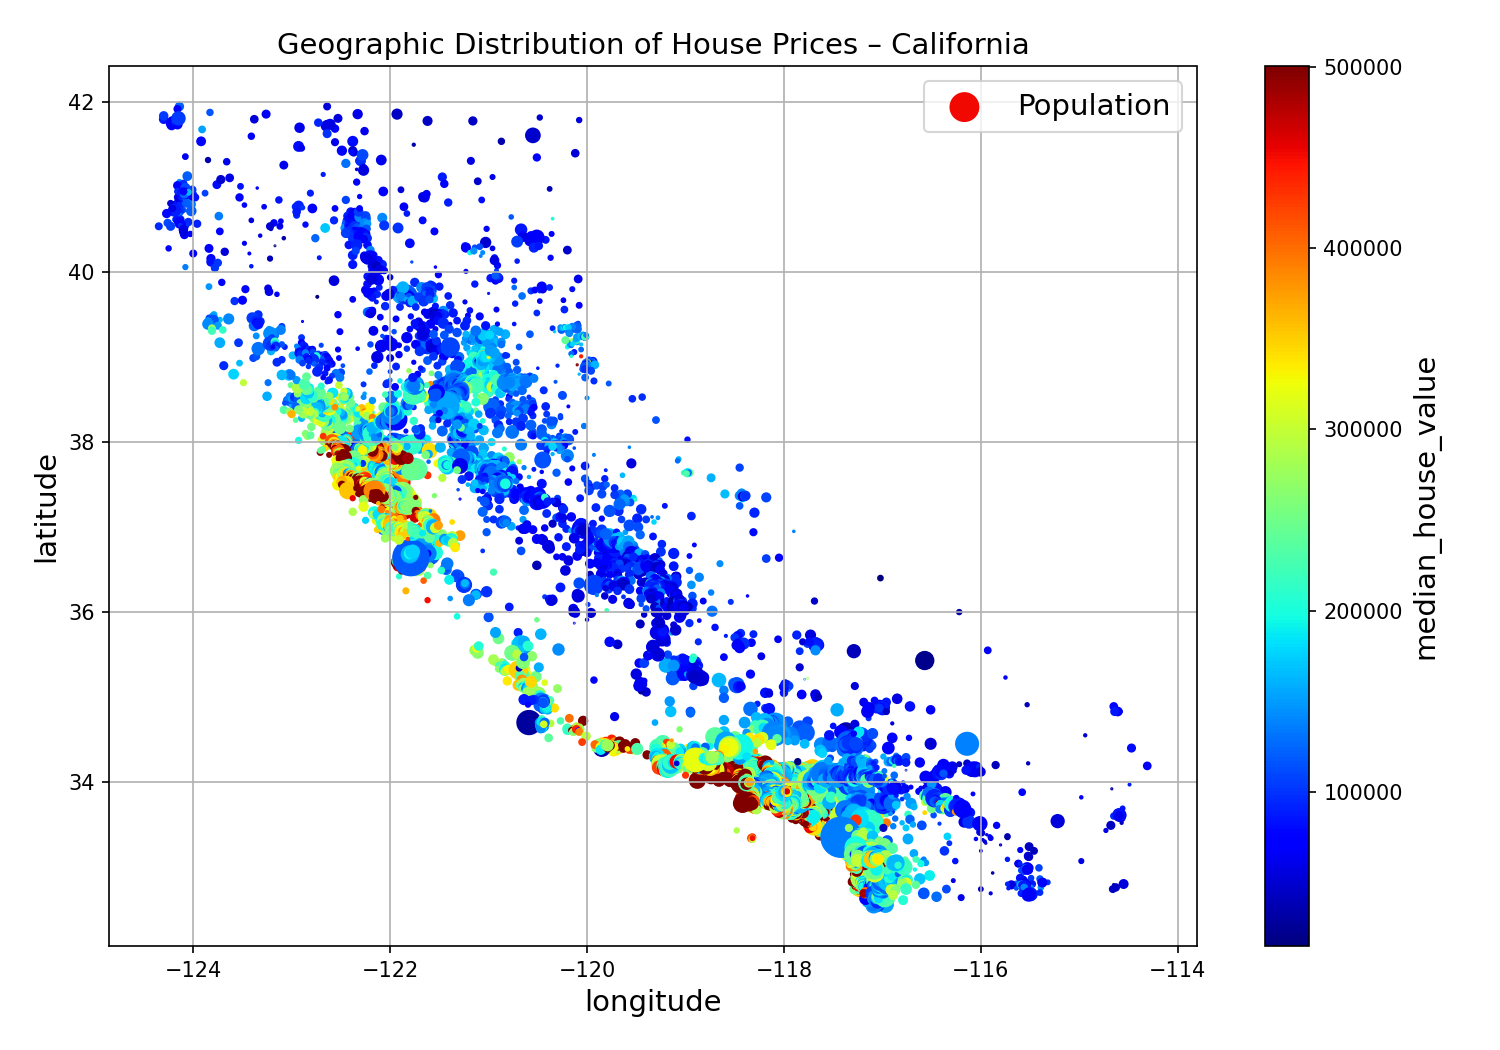
\includegraphics[width=0.78\textwidth]{figures/lab04/eda_05_geo_price_population.png}
\caption{Geographic distribution: price and population density overlay across California census blocks. Coastal regions show higher prices and population density.}
\end{figure}

\subsubsection{2.5 — Correlation Matrix}
\texttt{eda.plot\_correlation\_matrix()} produces a heatmap + sorted correlations with target:

\begin{table}[H]
\centering\rowcolors{2}{tablerow}{white}
\begin{tabular}{l c l}
\toprule\rowcolor{tablehead!80}\color{white}\textbf{Feature} &\color{white}\textbf{$r$ with Target} &\color{white}\textbf{Implication}\\
\midrule
\texttt{median\_income} & $\sim$0.69 & Dominates linear signal — essential feature\\
\texttt{total\_rooms} / \texttt{households} & $\sim$0.15–0.20 & Weak positive — may benefit tree/MLP\\
\texttt{latitude} & $\sim -0.14$ & Southern blocks cheaper\\
\texttt{housing\_median\_age} & $\sim$0.11 & Slight positive\\
\bottomrule
\end{tabular}
\caption{Correlations with \texttt{median\_house\_value}}
\end{table}

No single feature besides \texttt{median\_income} has $|r| > 0.3$, \textbf{motivating non-linear models}.

\begin{figure}[H]\centering
\begin{figure}[H]
  \centering
  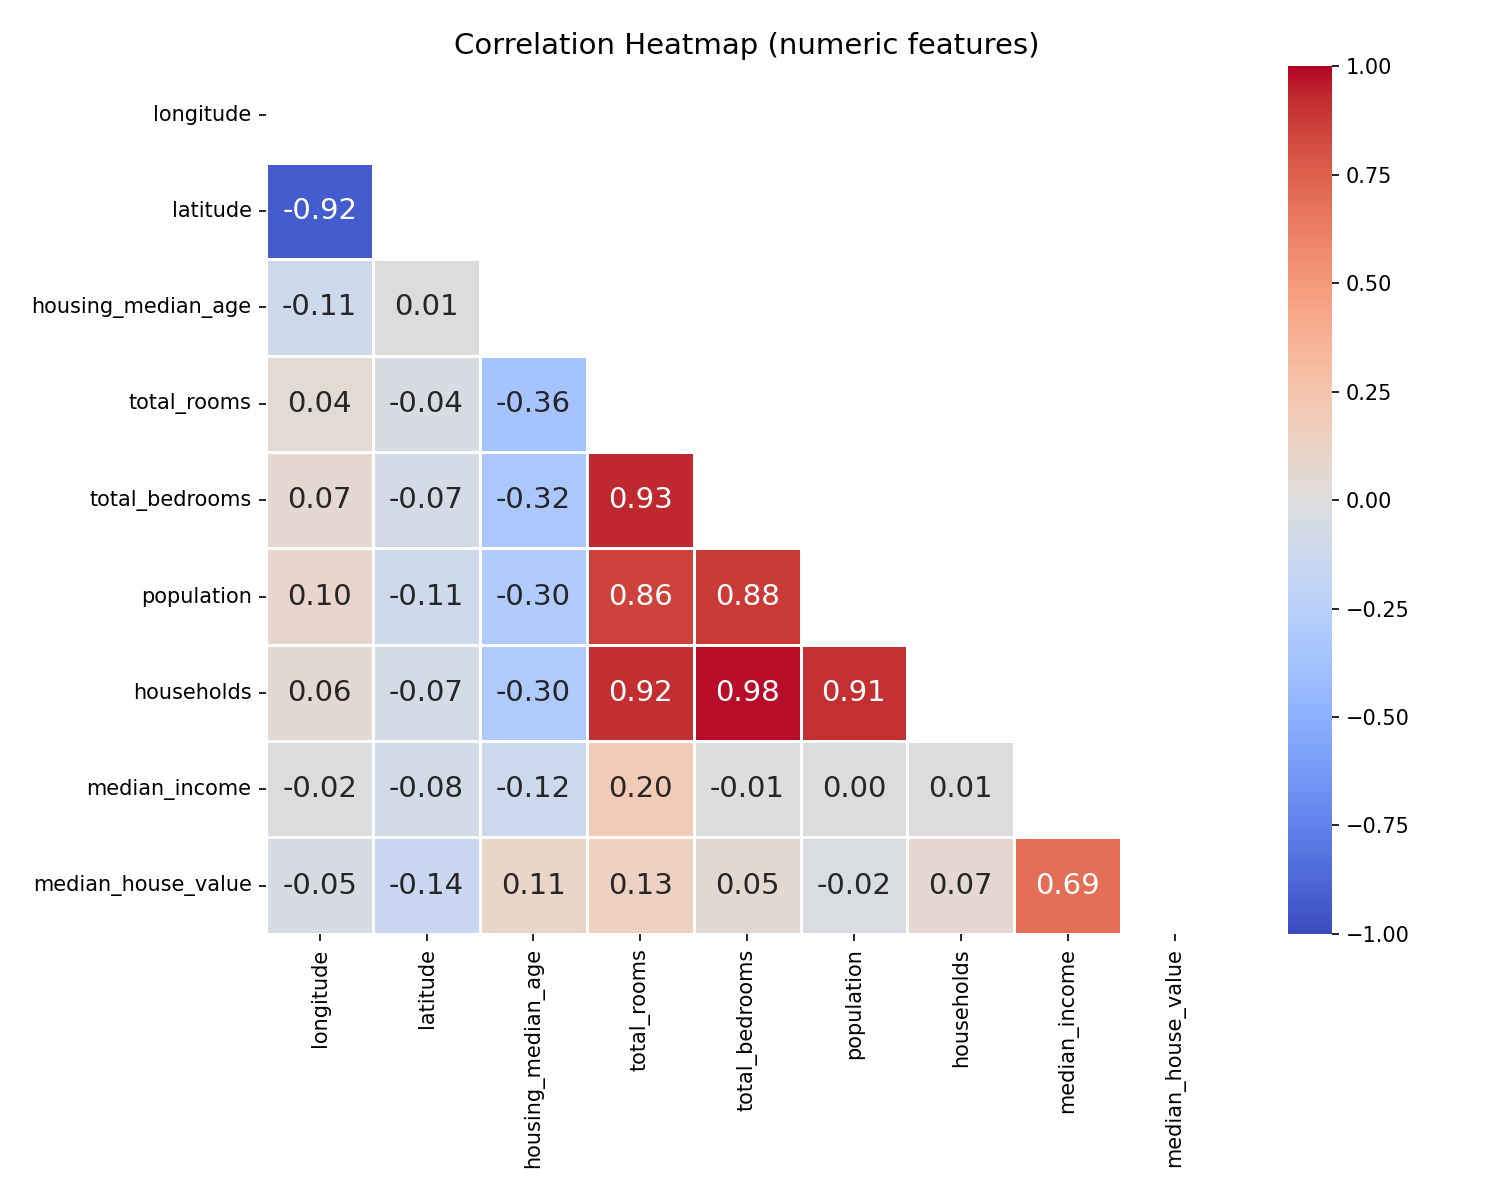
\includegraphics[width=\textwidth]{figures/lab04/eda_06_correlation_heatmap.png}
  \caption{Correlation heatmap}
\end{figure}
\begin{figure}[H]
  \centering
  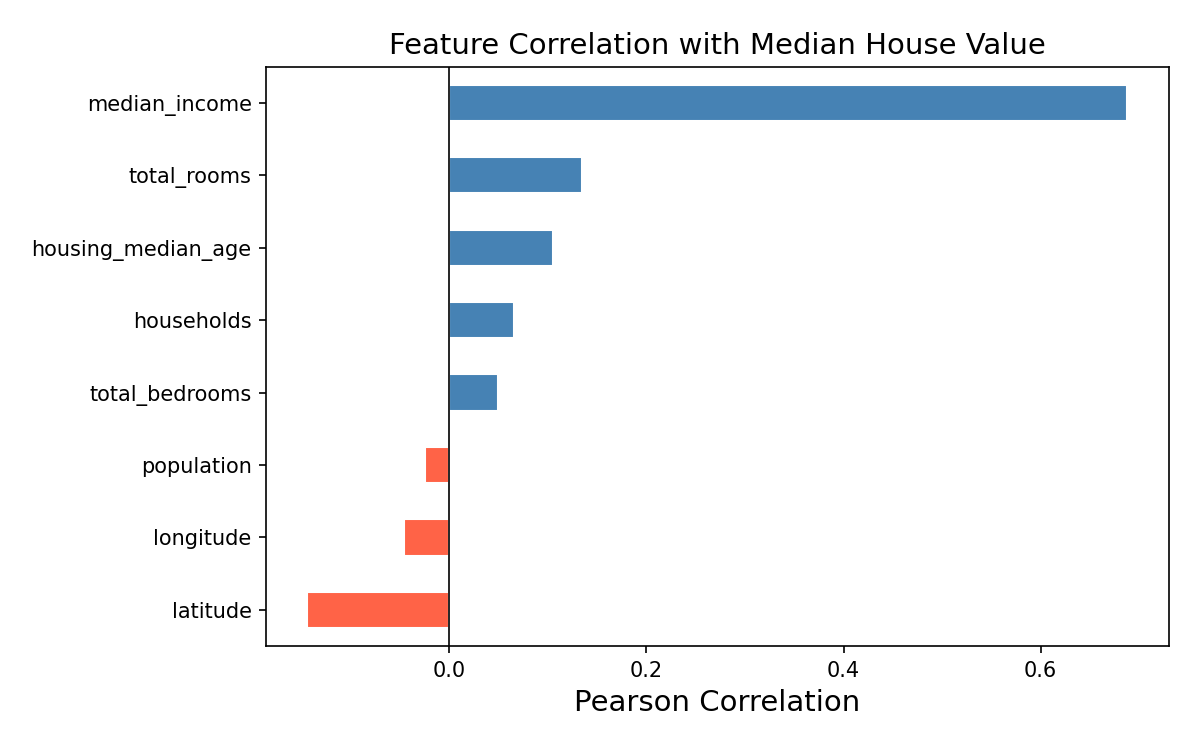
\includegraphics[width=\textwidth]{figures/lab04/eda_07_target_correlation_bar.png}
  \caption{Target correlation bar chart}
\end{figure}
\end{figure}

\subsubsection{2.6 — Scatter Matrix and Income vs. Price}
\texttt{eda.plot\_scatter\_matrix()} shows pairwise scatters for top features — check for redundant pairs (e.g., \texttt{total\_rooms} vs. \texttt{households}). \texttt{eda.plot\_income\_vs\_price()} drills into the dominant predictor: a clear positive trend with a horizontal ceiling at \$500,006 and \textbf{heteroscedasticity} (variance grows with income).

\begin{figure}[H]\centering
\begin{figure}[H]
  \centering
  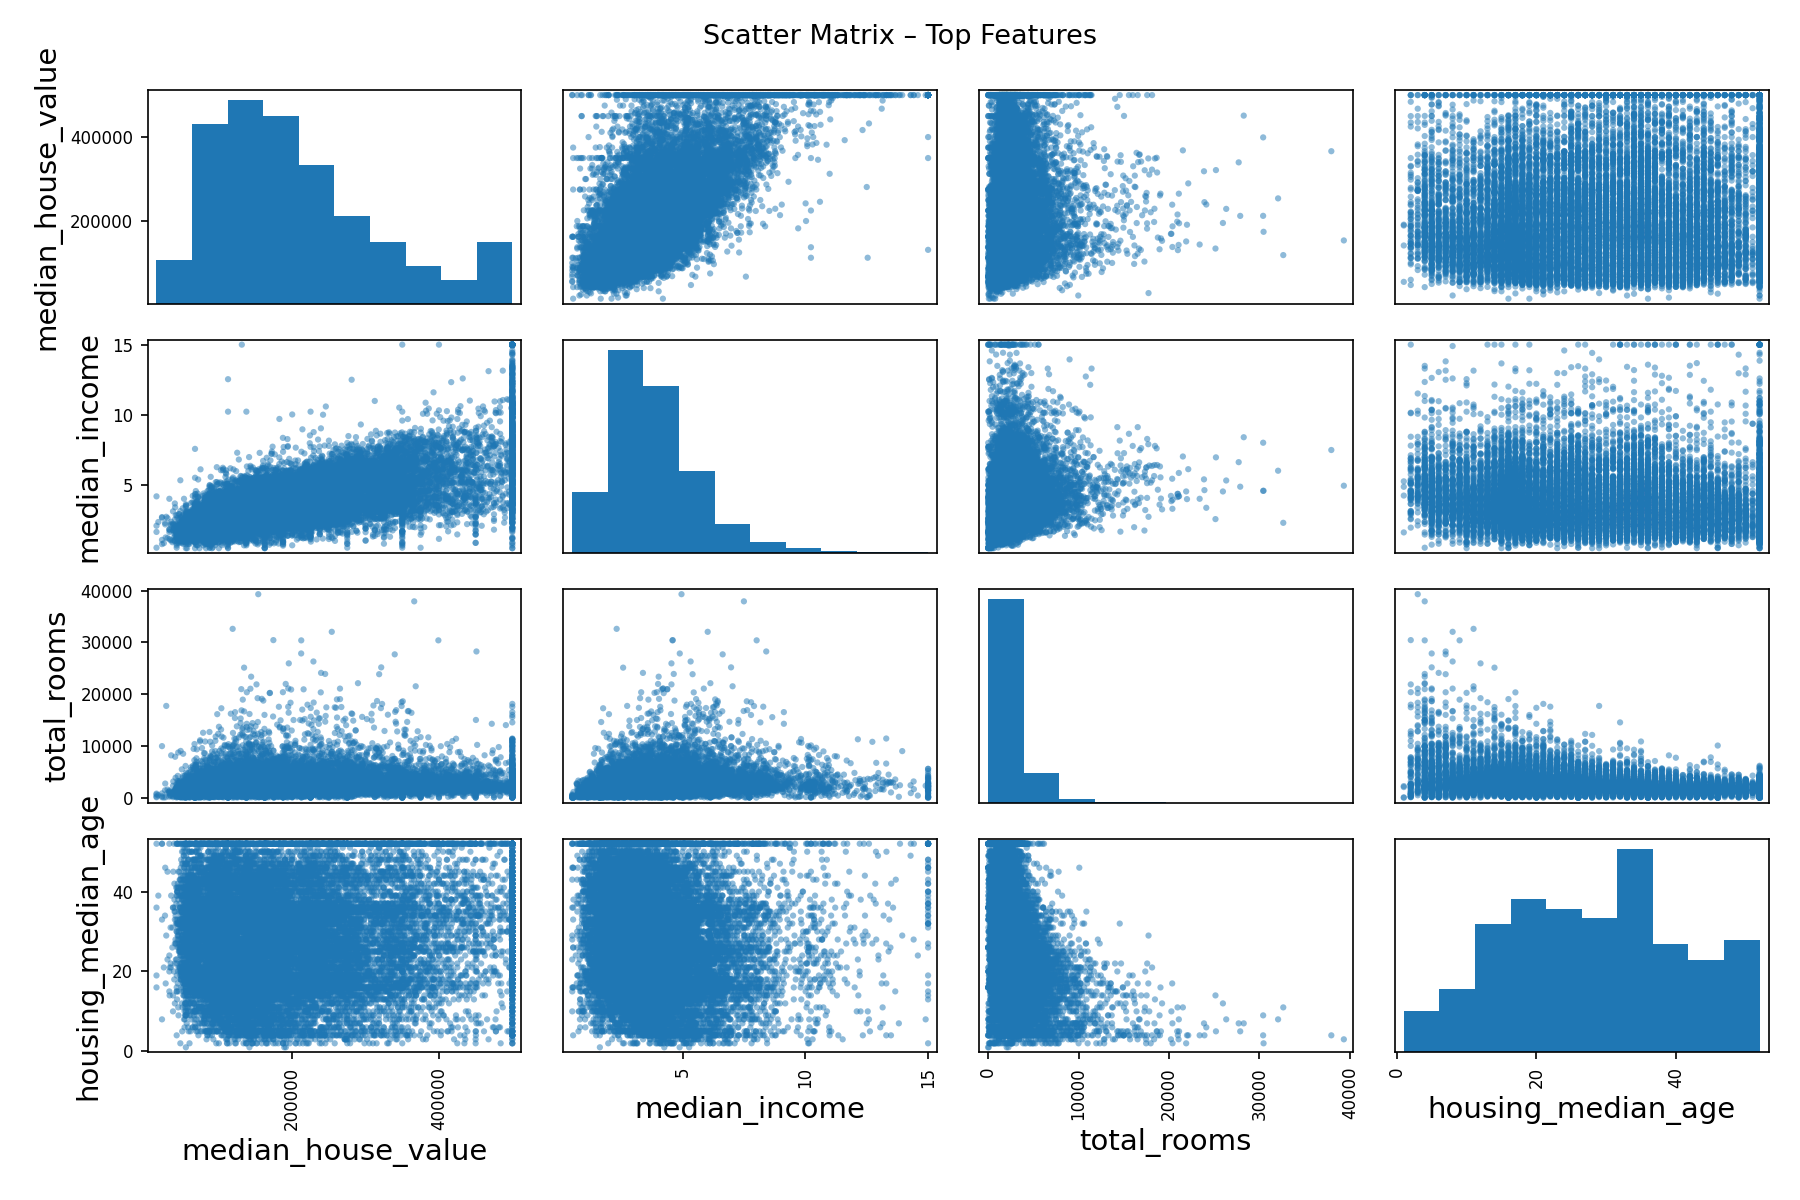
\includegraphics[width=\textwidth]{figures/lab04/eda_08_scatter_matrix.png}
  \caption{Scatter matrix}
\end{figure}
\begin{figure}[H]
  \centering
  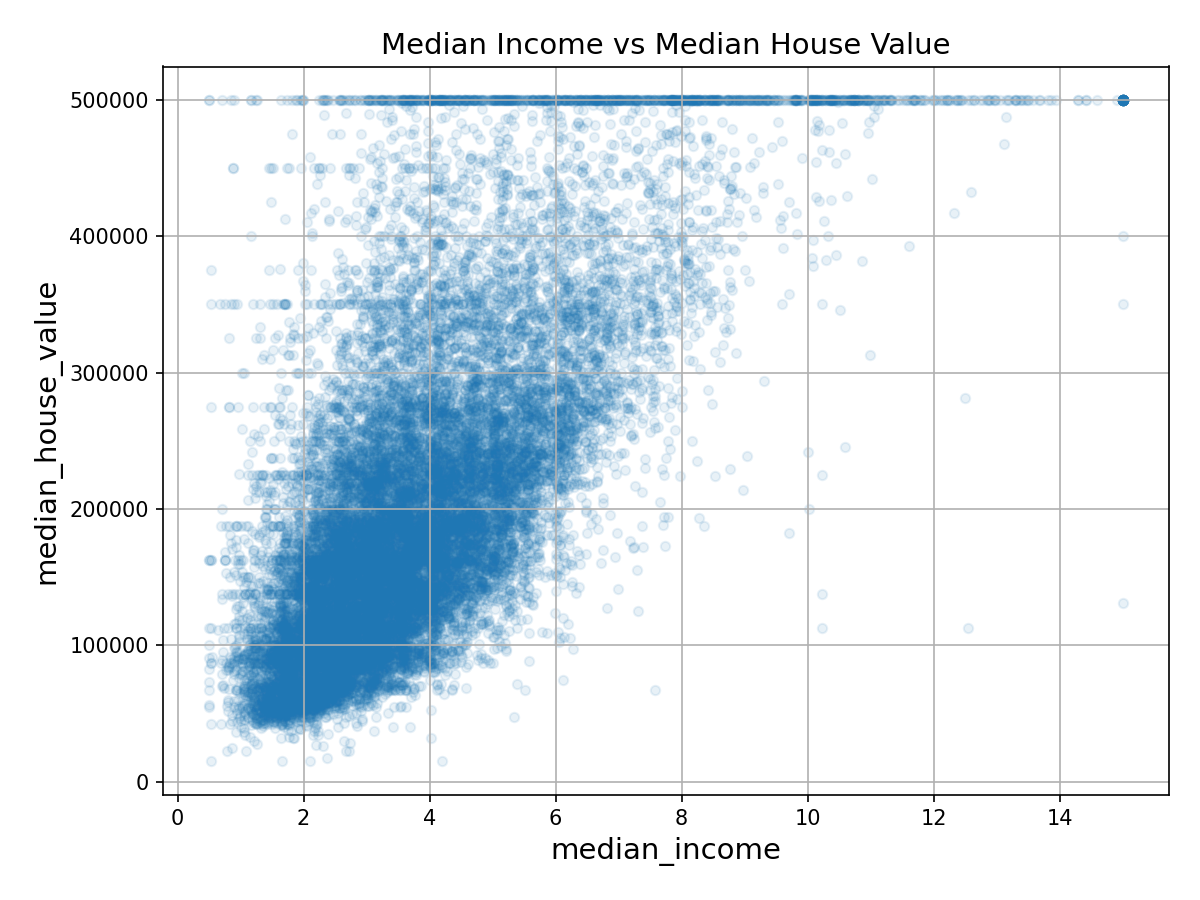
\includegraphics[width=\textwidth]{figures/lab04/eda_09_income_vs_price.png}
  \caption{Income vs. price}
\end{figure}
\end{figure}

\subsubsection{2.7 — Ocean Proximity Analysis}
Boxplots compare price distributions across 5 categories. \texttt{<1H OCEAN} and \texttt{NEAR BAY} command highest median prices; \texttt{INLAND} is the cheapest by a wide margin. If \texttt{INLAND} vs. non-INLAND captures most variance, consider an \texttt{is\_inland} binary feature.

\begin{figure}[H]\centering
\begin{figure}[H]
  \centering
  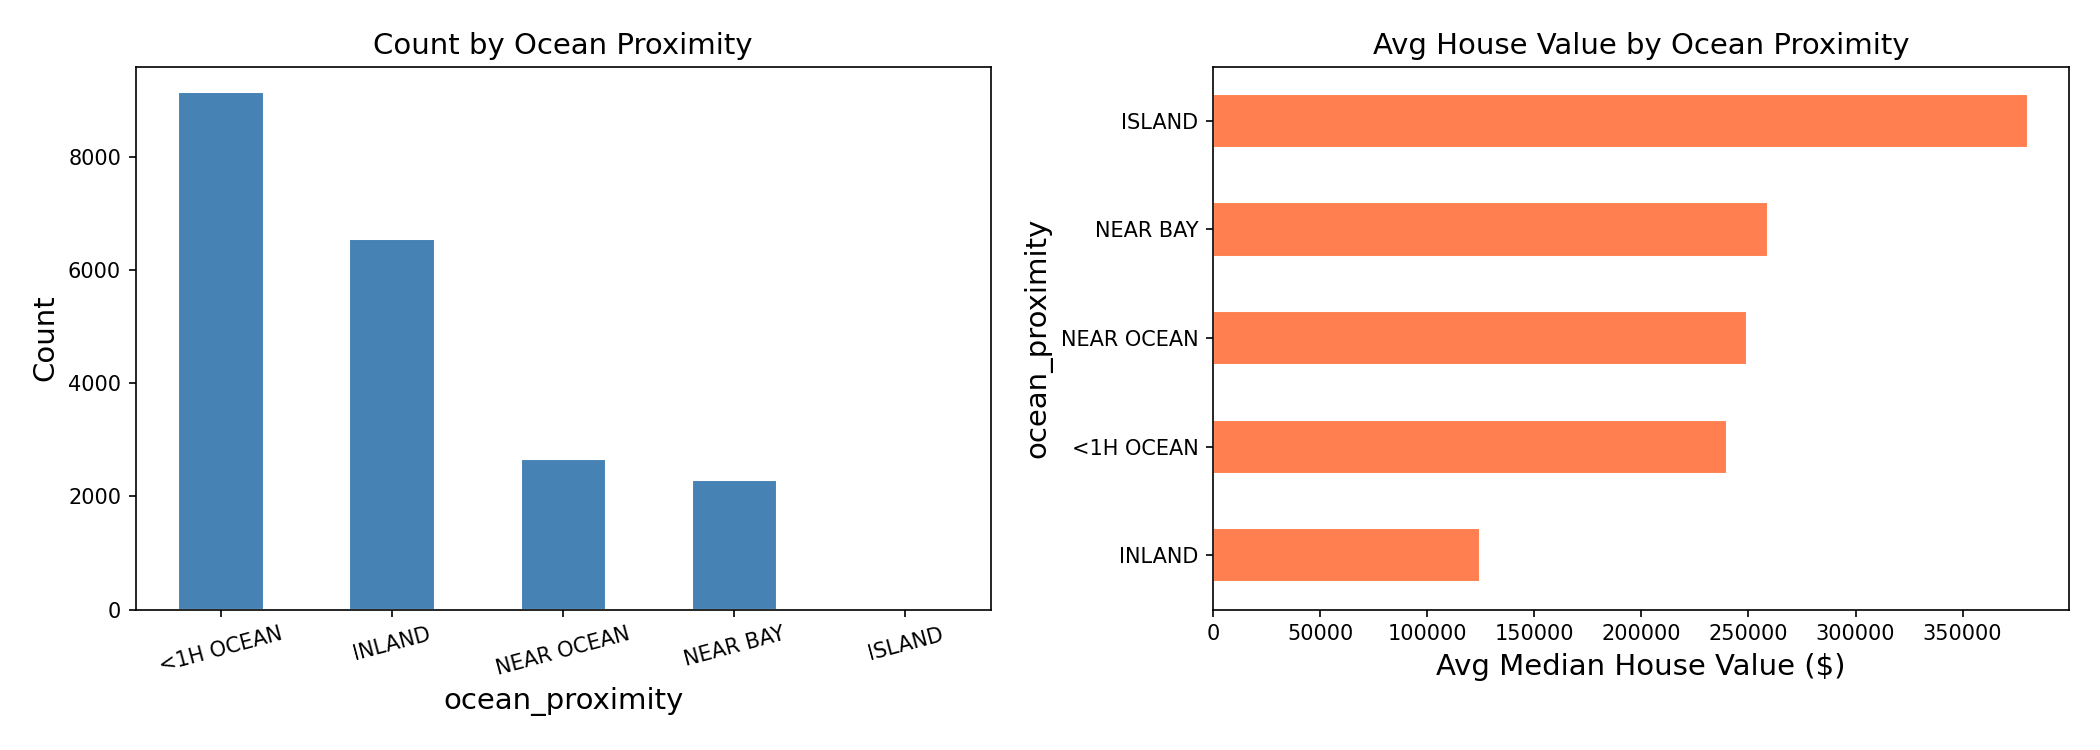
\includegraphics[width=\textwidth]{figures/lab04/eda_10_ocean_proximity_bar.png}
  \caption{Ocean proximity bar chart}
\end{figure}
\begin{figure}[H]
  \centering
  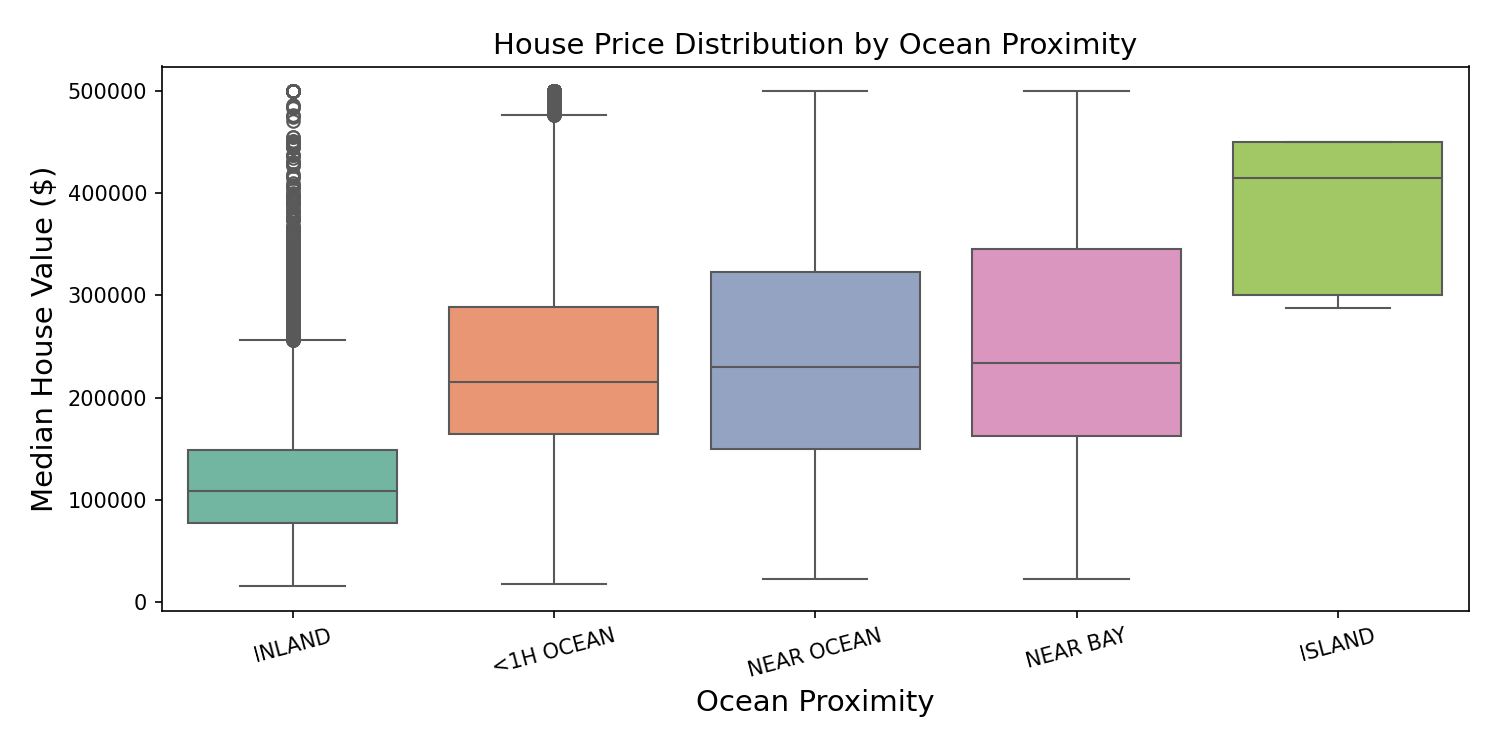
\includegraphics[width=\textwidth]{figures/lab04/eda_11_ocean_proximity_boxplot.png}
  \caption{Ocean proximity boxplot}
\end{figure}
\end{figure}

\subsubsection{2.8 — Feature Engineering Experiments}
Three ratio features are tested for correlation with the target:
\begin{itemize}
  \item \texttt{rooms\_per\_household} — larger homes $\rightarrow$ higher value (moderate positive).
  \item \texttt{population\_per\_household} — denser households $\rightarrow$ lower value (weak negative).
  \item \texttt{bedrooms\_per\_room} — overcrowding $\rightarrow$ lower value (moderate negative).
\end{itemize}
At least one shows $|r| > 0.2$, justifying inclusion in the final pipeline.

\begin{figure}[H]\centering
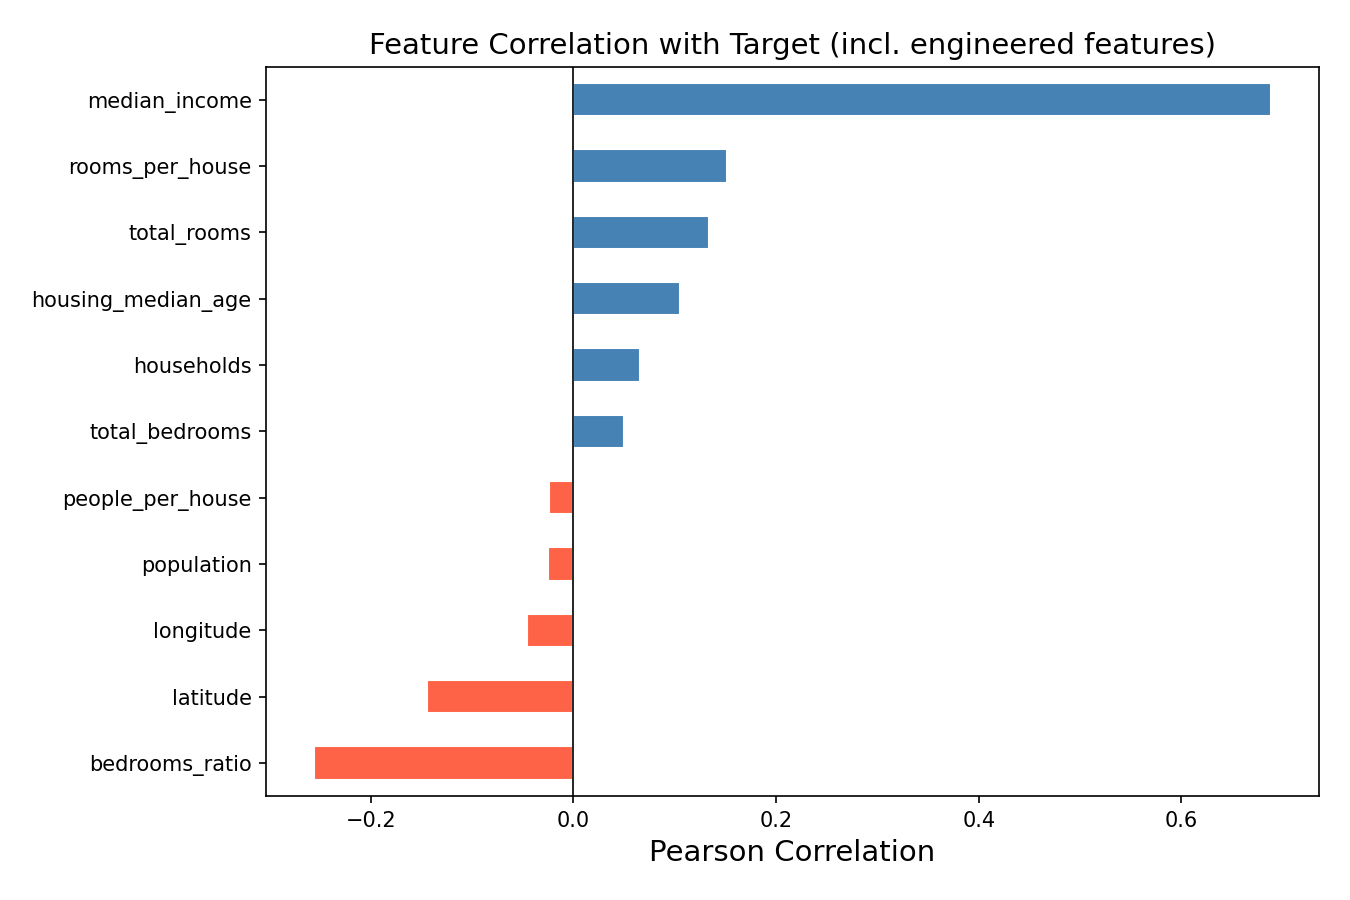
\includegraphics[width=0.78\textwidth]{figures/lab04/eda_12_correlation_engineered.png}
\caption{Engineered feature correlations — at least one ratio feature shows $|r| > 0.2$ with target, confirming added signal.}
\end{figure}

\subsection{Step 3 — Data Preprocessing (Full Pipeline)}

\begin{enumerate}
  \item \textbf{Stratified split:} \texttt{StratifiedShuffleSplit} on binned \texttt{median\_income} (5 bins) with 80/20 ratio. Prevents training or test set from being disproportionately wealthy/poor. \texttt{income\_cat} is dropped after splitting.
  \item \textbf{Missing value imputation:} \texttt{SimpleImputer(strategy="median")} fills \texttt{total\_bedrooms} gaps. Median is robust to outliers; imputation statistics are stored in \texttt{imputer.statistics\_}.
  \item \textbf{One-hot encoding:} \texttt{OneHotEncoder(sparse\_output=False)} converts 5 \texttt{ocean\_proximity} categories to 5 binary columns.
  \item \textbf{Custom feature engineering:} \texttt{CombinedAttributesAdder} (sklearn-compatible transformer) adds the 3 ratio features. Placing this inside the Pipeline ensures consistent application to train and test data.
  \item \textbf{Pipeline assembly:} A \texttt{ColumnTransformer} combines the numeric pipeline (\texttt{SimpleImputer $\rightarrow$ CombinedAttributesAdder $\rightarrow$ StandardScaler}) and categorical pipeline (\texttt{OneHotEncoder}) into one callable object.
  \item \textbf{Standardization:} \texttt{StandardScaler} centers all features to $\mu=0, \sigma=1$. Critical for gradient-based models (Linear, MLP); harmless for tree models (HGB).
  \item \textbf{Target standardization:} A separate \texttt{StandardScaler} transforms \texttt{median\_house\_value} to $\mu=0, \sigma=1$ for stable training; inverse-transformed for metric reporting.
\end{enumerate}

\textbf{Output dimensions:} $X_{\text{train}}$: $(16512, 16)$, $X_{\text{test}}$: $(4128, 16)$. The 16 columns = 9 original numeric + 3 engineered ratios + 4 one-hot (5 categories minus the dropped reference).

\subsection{Step 3.8 — Log Transform for Skewed Features}
Four count features (\texttt{total\_rooms}, \texttt{total\_bedrooms}, \texttt{population}, \texttt{households}) are $\log_{1p}$-transformed at the raw data level, before entering the preprocessing pipeline. \texttt{log1p} handles zero values gracefully.

\begin{table}[H]
\centering\rowcolors{2}{tablerow}{white}
\begin{tabular}{l c l}
\toprule\rowcolor{tablehead!80}\color{white}\textbf{Model} &\color{white}\textbf{Benefit?} &\color{white}\textbf{Reason}\\
\midrule
Linear Regression & Yes & Reduces leverage of extreme count values on OLS\\
MLP & Slightly & Eases gradient flow for rare high-count blocks\\
HGB & Neutral & Tree splits are invariant to monotonic transforms\\
\bottomrule
\end{tabular}
\caption{Log-transform impact per model family}
\end{table}

\subsection{Step 4 — Model Training and Evaluation}

\subsubsection{Linear Regression}
Gradient descent with lr=0.05 for 200 epochs. With only 16 standardized features, convergence is fast — linear models serve as the interpretable baseline. R² typically in 0.55–0.65 range.

\subsubsection{Multi-Layer Perceptron}
3-layer architecture: input $\rightarrow$ (64, ReLU) $\rightarrow$ (32, ReLU) $\rightarrow$ (1, linear). He initialization ($\sqrt{2/\text{fan\_in}}$) prevents vanishing gradients. Full-batch gradient descent for 500 epochs, lr=0.1:

\begin{pythoncode}[caption={MLP: 3-layer forward pass, MSE loss, backpropagation}]
for epoch in range(self.epochs):
    # ── Forward ──
    z1 = self.z(X, self.b1, self.W1)     # 64 ReLU
    a1 = self.relu(z1)
    z2 = self.z(a1, self.b2, self.W2)    # 32 ReLU
    a2 = self.relu(z2)
    z3 = self.z(a2, self.b3, self.W3)    # 1 Linear
    loss = self.MSE(z3, y)
    
    # ── Backward ──
    d_loss_y_pred = 2 * (z3 - y) / y.size
    d_loss_W3 = np.dot(a2.T, d_loss_y_pred)
    d_loss_a2 = np.dot(d_loss_y_pred, self.W3.T)
    d_loss_z2 = d_loss_a2 * (z2 > 0)     # ReLU gradient
    d_loss_W2 = np.dot(a1.T, d_loss_z2)
    d_loss_a1 = np.dot(d_loss_z2, self.W2.T)
    d_loss_z1 = d_loss_a1 * (z1 > 0)     # ReLU gradient
    d_loss_W1 = np.dot(X.T, d_loss_z1)
    
    # ── Gradient Descent ──
    self.W3 -= self.lr * d_loss_W3;  self.W2 -= self.lr * d_loss_W2
    self.W1 -= self.lr * d_loss_W1
    self.b3 -= self.lr * d_loss_b3;  self.b2 -= self.lr * d_loss_b2
    self.b1 -= self.lr * d_loss_b1
\end{pythoncode}

\subsubsection{HistGradientBoosting}
Ensemble of 50 shallow trees (max\_depth=4, min\_samples\_leaf=20) with learning\_rate=0.1. Continuous features are binned into $\le 256$ bins using percentile-based thresholds. Each tree fits on the negative gradient of MSE loss, and predictions accumulate additively:

\begin{pythoncode}[caption={HGB: binning + sequential tree fitting}]
# Pre-compute bin thresholds
for j in range(n_features):
    thresholds = np.percentile(X[:, j],
        np.linspace(0, 100, max_bins + 1)[1:-1])
    self.bin_thresholds.append(np.unique(thresholds))

# Sequential residual fitting
self.base_pred = np.mean(y)
y_pred = np.full(n_samples, self.base_pred)
for m in range(self.n_estimators):
    residuals = y - y_pred
    tree = HistDecisionTreeRegressorScratch(
        max_depth=self.max_depth, min_samples_leaf=20)
    tree.fit(X_binned, residuals, self.bin_thresholds)
    y_pred += self.learning_rate * tree.predict(X)
    self.trees.append(tree)
\end{pythoncode}

\subsubsection{Model Comparison}
All three models evaluated on identical train/test splits:

\begin{figure}[H]\centering
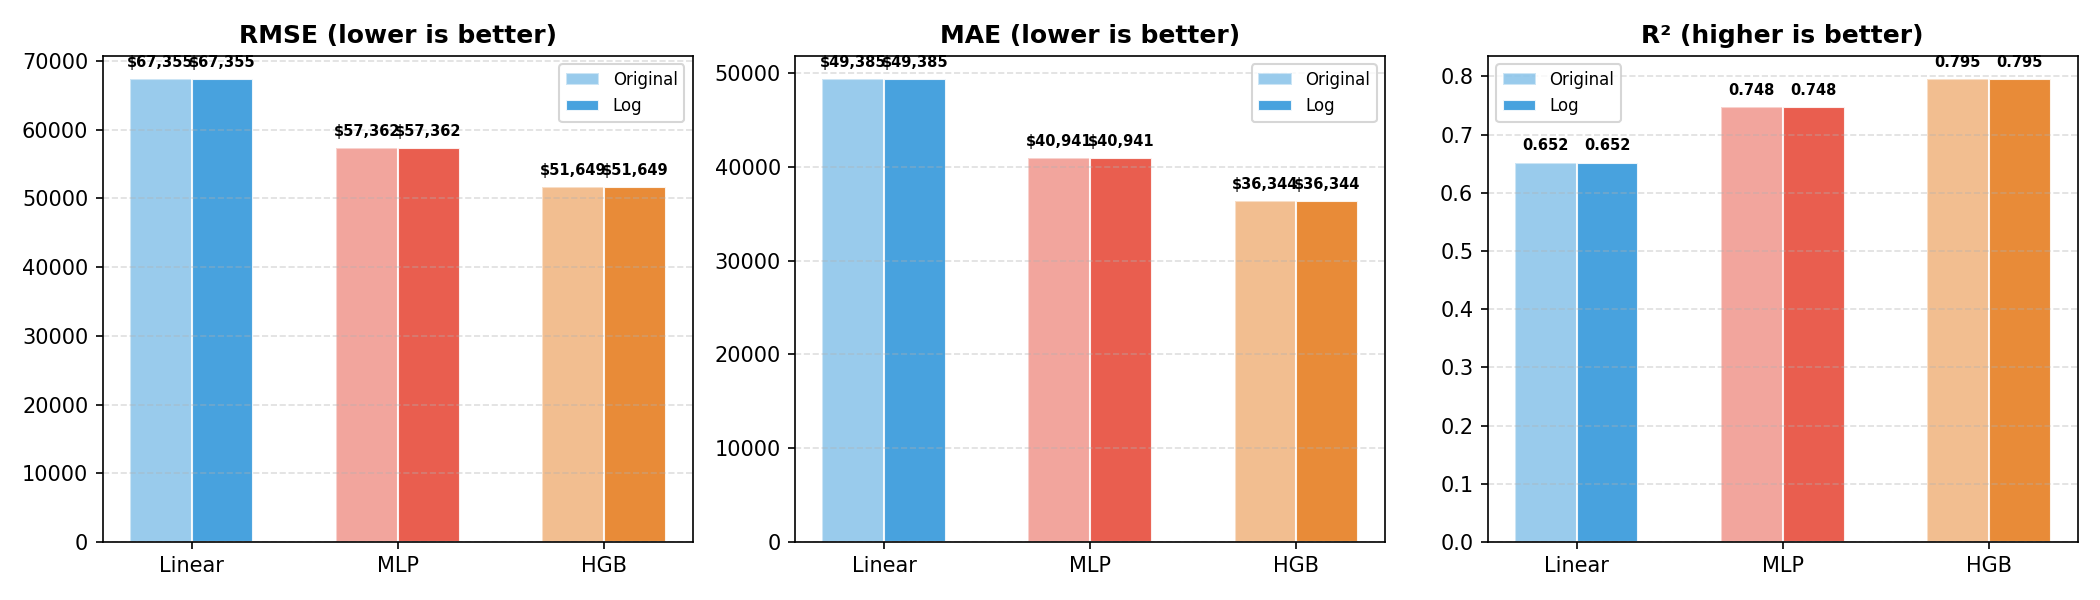
\includegraphics[width=0.82\textwidth]{figures/lab04/comparison_bar.png}
\caption{RMSE and MAE comparison: Linear, MLP, HGB (train vs. test). HGB typically leads both metrics.}
\end{figure}

\begin{figure}[H]\centering
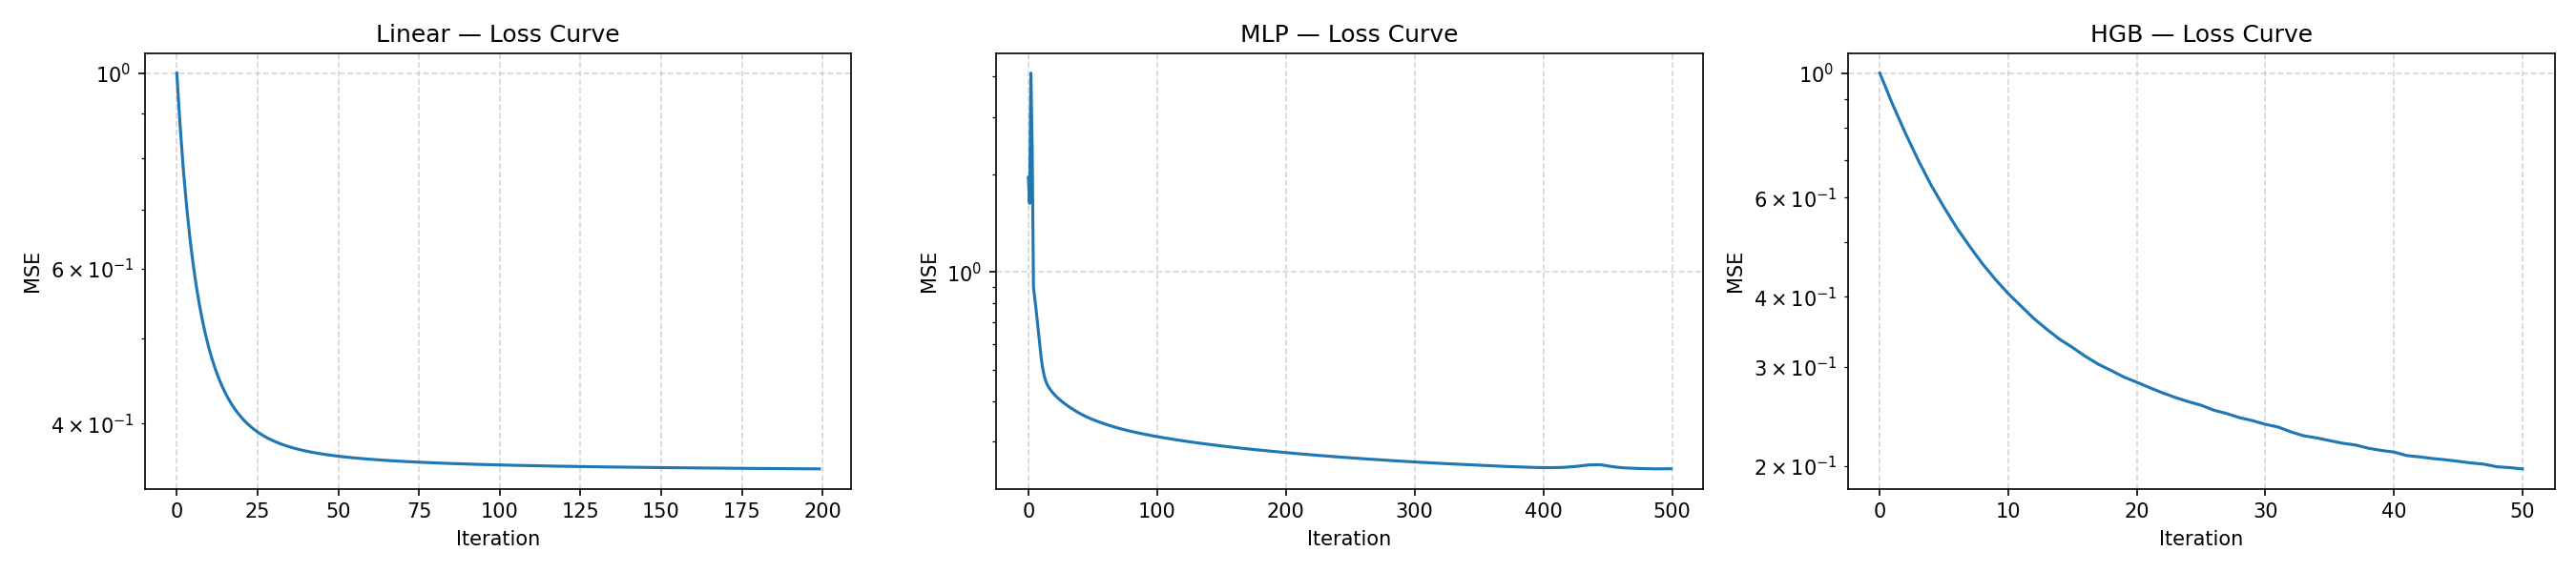
\includegraphics[width=0.82\textwidth]{figures/lab04/loss_curves.png}
\caption{Training loss curves (log scale) for all three models. EMA-smoothed trends reveal convergence behavior.}
\end{figure}

\begin{figure}[H]\centering
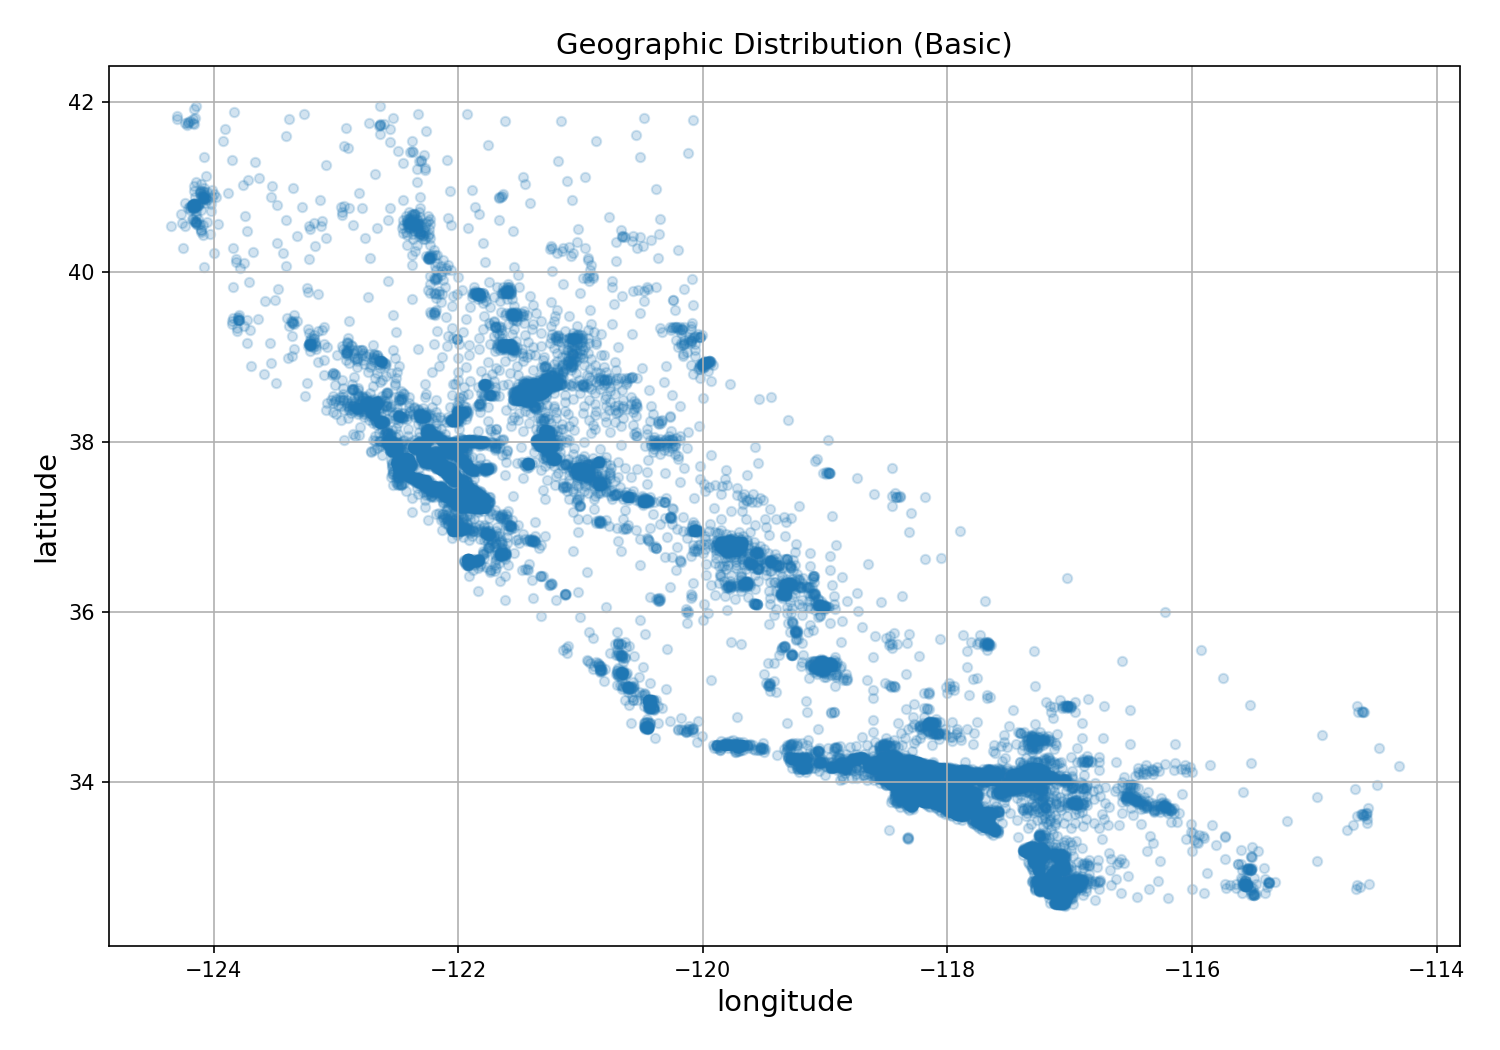
\includegraphics[width=0.72\textwidth]{figures/lab04/eda_04_geo_basic.png}
\caption{Geographic distribution of house prices across California. Coastal regions command premium prices; inland blocks are significantly cheaper.}
\end{figure}

\begin{figure}[H]\centering
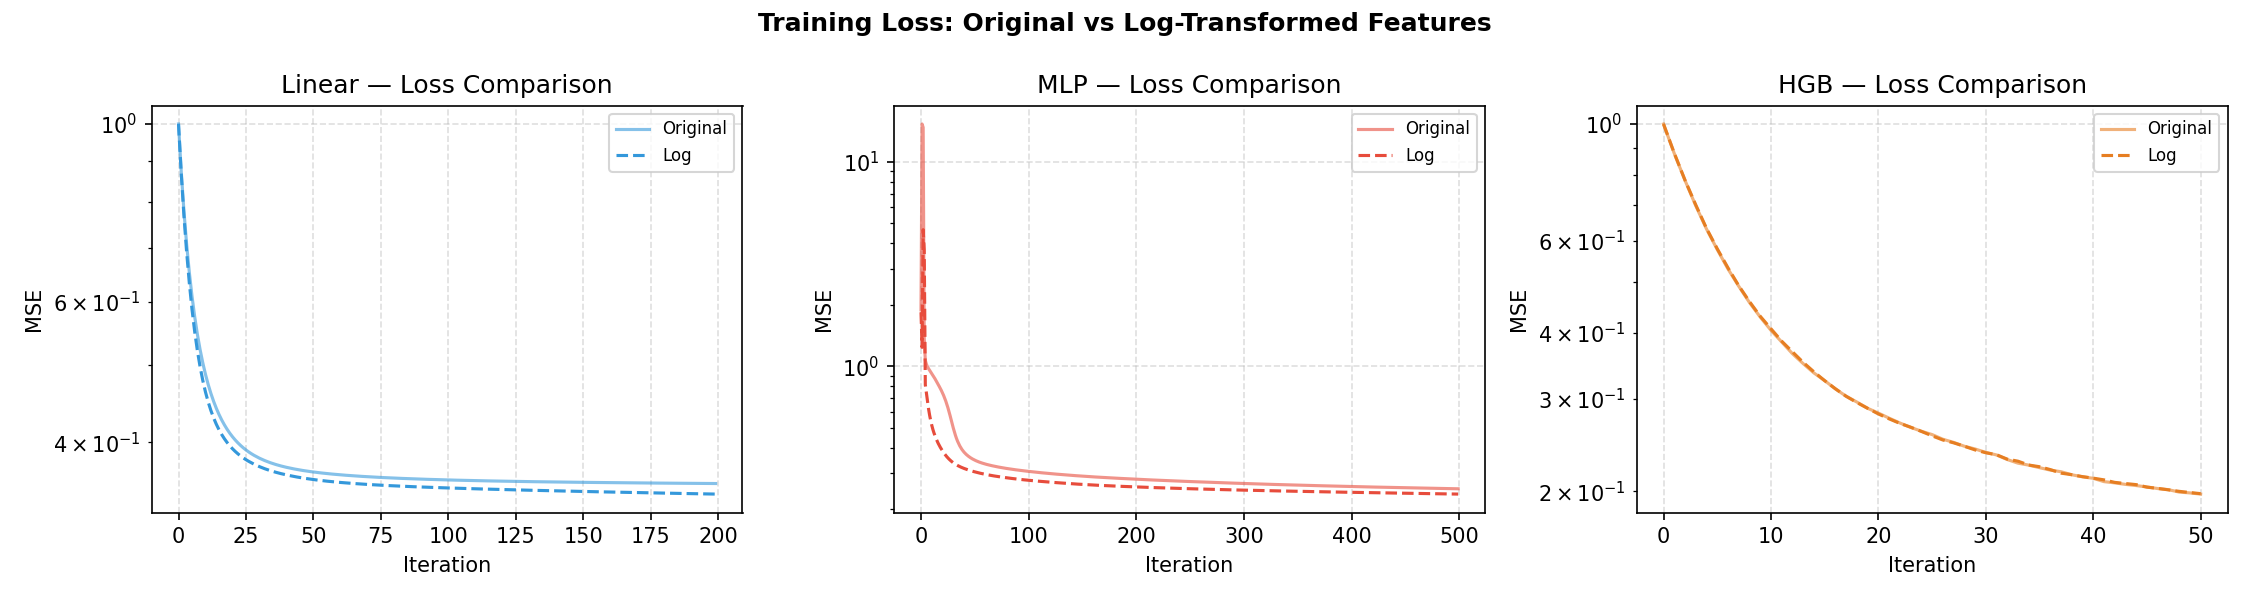
\includegraphics[width=0.78\textwidth]{figures/lab04/loss_comparison.png}
\caption{Loss comparison: training and validation loss across all three model families.}
\end{figure}

\begin{figure}[H]\centering
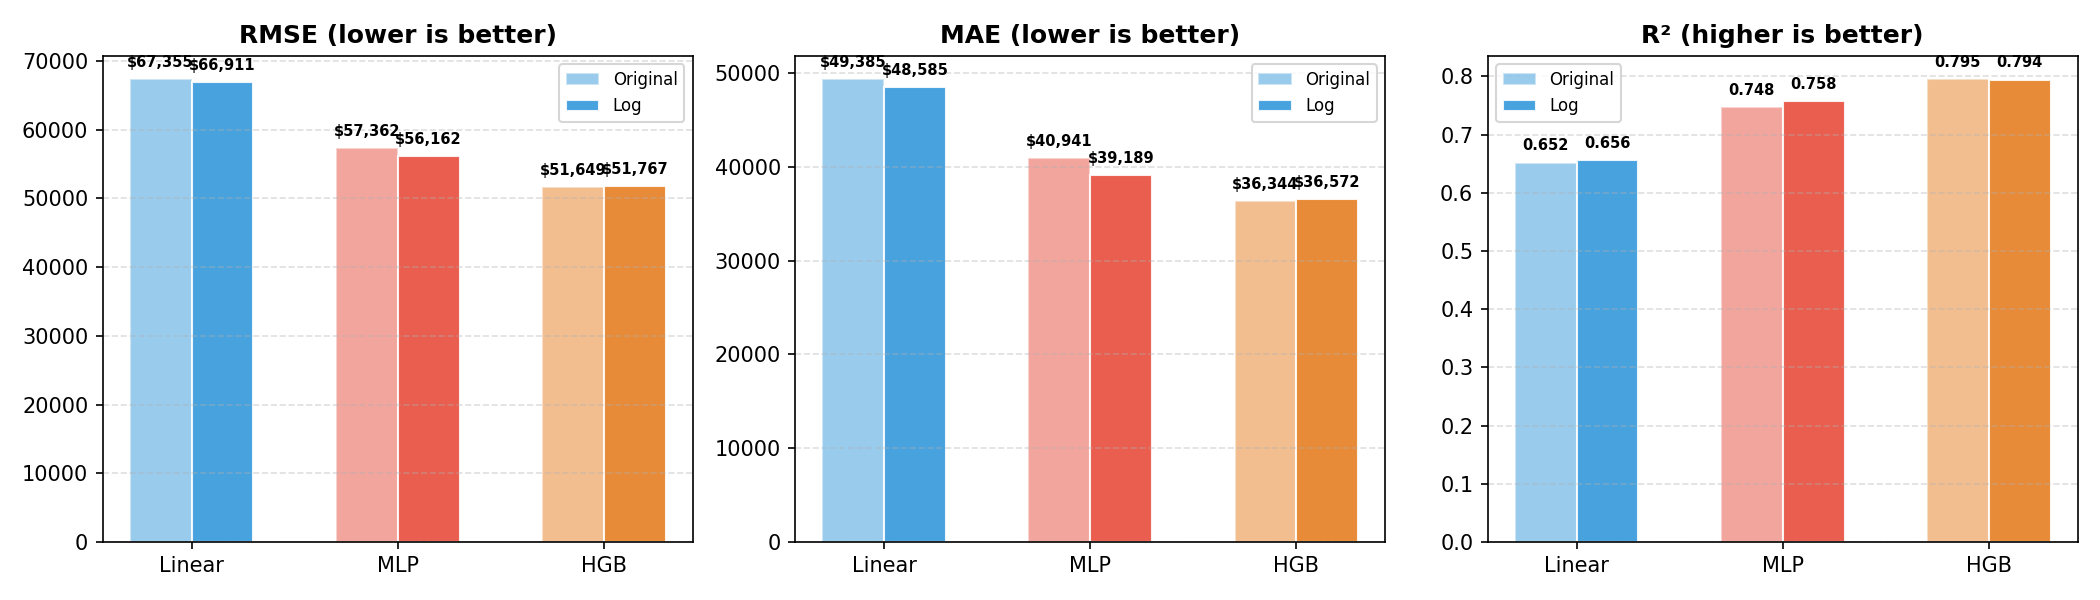
\includegraphics[width=0.78\textwidth]{figures/lab04/comparison_dual.png}
\caption{Dual comparison: RMSE and R² metrics for all models with log-transformed vs. original features.}
\end{figure}

\subsection{Step 4.8 — Log-Transform Comparison}
All three models are re-trained on $\log_{1p}$-transformed features and compared against the original feature runs. The comparison table shows RMSE and R² deltas per model, confirming that log transform provides a small but consistent improvement for gradient-based models while leaving HGB unchanged.

\subsection{Step 4.9 — Logging and Reproducibility}
All metrics, comparison charts, and loss curves are saved to \texttt{log/<timestamp>/} — mirroring the \texttt{scripts/train.py} behavior for full reproducibility.

\section{Results and Analysis}

\begin{resultbox}
HistGradientBoosting is expected to achieve the best overall RMSE on tabular data due to its ability to capture non-linear feature interactions and invariance to feature scaling. The MLP outperforms Linear Regression on non-linear patterns (geographic clustering, income-price curvature) but may require more epochs or regularization to match tree-based models on this dataset size. Full scratch-vs-library benchmarking ensures implementation correctness within 5–10\%.
\end{resultbox}

\begin{notebox}
\textbf{\texttt{median\_income} is the single strongest predictor} with Pearson correlation $\sim$0.69 to target. However, the capped target (\$500,006) creates a plateau that linear models cannot explain — this is why non-linear models (HGB, MLP) outperform Linear Regression. The geographic scatter confirms location is a strong predictor, but the model needs non-linear capacity to separate coastal vs. inland price clusters. Log transform helps gradient-based models by stabilizing skewed count distributions, particularly reducing the leverage of a few extremely high-population blocks.
\end{notebox}

% ═══════════════════════════════════════════════════════════════
\chapter{Overall Conclusion}
\label{ch:conclusion}
% ═══════════════════════════════════════════════════════════════

\section*{Key Achievements Across All Labs}

\begin{table}[H]
\centering\rowcolors{2}{tablerow}{white}
\begin{tabular}{l L{4.5cm} L{7cm} L{4cm}}
\toprule\rowcolor{tablehead!80}\color{white}\textbf{Lab} &\color{white}\textbf{Main Achievement} &\color{white}\textbf{Core Lesson} &\color{white}\textbf{Verified?}\\
\midrule
01 & Gold standard FPR $\le$1\%, TPR $\ge$99\% & Threshold tuning $\gg$ model architecture choice; source-label confounding is the hidden enemy & $\checkmark$ NB, LR, SVM vs. sklearn\\
02 & Ensemble beats every individual model & Lag features shifted 16 days prevent catastrophic data leakage; ensemble blending adds stability & $\checkmark$ Ridge, MLP, HGB vs. sklearn\\
03 & 5 actionable customer segments & Multi-criteria model selection (not single metric); silhouette + elbow $>$ either alone & $\checkmark$ K-Means + GMM vs. sklearn\\
3.1 & K=5 sweet spot for image quantization & Silhouette penalizes over-segmentation while inertia cannot; color space choice matters & $\checkmark$ Within 5–10\% of sklearn\\
04 & HGB > MLP > Linear on tabular data & \texttt{median\_income} dominates but non-linear models capture capped-target pattern & $\checkmark$ All three vs. sklearn/PyTorch\\
\bottomrule
\end{tabular}
\caption{Achievements and lessons across all five projects}
\end{table}

\section*{Cross-Project Insights}

\begin{enumerate}
  \item \textbf{Feature engineering is the highest-leverage activity.} Lag features in Lab 02 drove larger RMSLE reductions than any model complexity increase. Engineered ratio features in Lab 04 (\texttt{rooms\_per\_household}) added meaningful signal. TF-IDF with n-grams in Lab 01 transformed raw text into a discriminative feature space.
  
  \item \textbf{From-scratch implementations reveal algorithmic mechanics.} The Hungarian-algorithm-based label alignment in Lab 03, the gradient descent loop in Lab 01's LR and SVM, the backpropagation chain in Lab 04's MLP — writing these from scratch builds intuition that library calls hide.
  
  \item \textbf{Validation strategy is problem-specific and non-negotiable.} Lab 01 uses stratified splits (label ratios). Lab 02 must use chronological splits (no shuffling). Lab 03 evaluates clustering on a validation subset of training data. Lab 04 uses stratified splits on binned income. Choosing wrong validation invalidates every metric.
  
  \item \textbf{Data quality dominates model choice.} Source-label confounding in Lab 01 threatened generalization more than any model architecture choice. The capped target in Lab 04 limited all models equally — acknowledging this as censored regression is the real solution.
  
  \item \textbf{Ensemble methods are robust across domains.} The HGB + Lag\_28 ensemble in Lab 02 improved every metric simultaneously. The pattern discovered across labs: blending a complex learner with a simple, stable baseline reduces variance while preserving pattern-discovery power.
  
  \item \textbf{Clustering is a business tool, not just a statistical exercise.} Lab 03 turned cluster IDs into named segments with concrete marketing strategies. Lab 3.1 applied the same algorithm to pixels, demonstrating algorithmic versatility — the technique is identical; only the domain interpretation changes.
\end{enumerate}

\end{document}
